% =====================================
% Accessible PDF Setup (Overleaf Safe)
% =====================================

\ifdefined\DocumentMetadata
  \DocumentMetadata{
    lang=en-US
  }
\fi

\documentclass[12pt,reqno,oneside]{amsbook}

% =====================================
% Encoding (required for screen readers)
% =====================================

\usepackage[T1]{fontenc}
\usepackage[utf8]{inputenc}

\ifdefined\pdfglyphtounicode
  \input{glyphtounicode}
  \pdfgentounicode=1
\fi

% =====================================
% Language
% =====================================

\usepackage[english]{babel}
\usepackage{latexml}

% =====================================
% Math
% =====================================

\usepackage{amsmath,amssymb,amsthm}

% =====================================
% Graphics
% =====================================

\usepackage{graphicx}
\usepackage{subcaption}

% =====================================
% Code
% =====================================

\iflatexml
\else
  \usepackage{listings}
\fi
\usepackage{comment}

% =====================================
% Layout
% =====================================

\usepackage{geometry}
\geometry{margin=1in}

% =====================================
% Spacing
% =====================================

\usepackage{setspace}

% =====================================
% Hyperlinks + PDF metadata
% =====================================

\usepackage[
 pdfusetitle,
 pdfencoding=auto,
 psdextra,
 colorlinks=true,
 linkcolor=black,
 citecolor=black,
 urlcolor=blue
]{hyperref}

% =====================================
% Tagged PDF (lightweight mode)
% =====================================

\iflatexml
  \providecommand{\tagpdfsetup}[1]{}
\else
  \usepackage{tagpdf}
  \tagpdfsetup{
   activate,
   interwordspace=true
  }
\fi

% =====================================
% Custom inputs
% =====================================

% This is the user manual for UICTHESI CLS, originally found
% at https://www.math.uic.edu/graduate/current/uicthesi, and
% modified by Pete Snyder <snyder@gmail.com> to match the
% current department requirements.
\usepackage{booktabs}
\usepackage{newlfont}
\usepackage{amsfonts}
\usepackage{amssymb}
\usepackage{euler}
\usepackage{xspace}
\usepackage{float}
\usepackage{flushend}
\usepackage{footnote}
\usepackage{enumitem}
\usepackage{url}
\usepackage{caption}
\usepackage{booktabs}
\usepackage{graphicx}
\usepackage[dvipsnames]{xcolor}
\usepackage{cite}
\usepackage{multirow}
\usepackage{tabularx}
\iflatexml
  \newcommand{\makecell}[2][]{\begin{tabular}[c]{@{}l@{}}#2\end{tabular}}
\else
  \usepackage{listings}
  \usepackage[xindy={glsnumbers=false},nonumberlist,acronym,nopostdot,nogroupskip,nomain]{glossaries}
  \usepackage[htt]{hyphenat}
  \usepackage{makecell}
  \usepackage{lipsum}
  \usepackage{tcolorbox}
  \usepackage{minted}
\fi

\iflatexml
\else
\newglossarystyle{clong}{%
 \renewenvironment{theglossary}%
     {\begin{longtable}{p{.2\linewidth}p{.8\linewidth}}}%
     {\end{longtable}}%
  \renewcommand*{\glossaryheader}{}%
  \renewcommand*{\glsgroupheading}[1]{}%
  \renewcommand*{\glossaryentryfield}[5]{%
    \glstarget{##1}{##2} & ##3\glspostdescription\space ##5\\}%
  \renewcommand*{\glossarysubentryfield}[6]{%
     & \glstarget{##2}{\strut}##4\glspostdescription\space ##6\\}%
  %\renewcommand*{\glsgroupskip}{ & \\}%
}
\fi

\makesavenoteenv{tabular}
\makesavenoteenv{table}

\iflatexml
\else
  \input{sections/other/__abbrs}
\fi
\def\new@fontshape#1#2#3#4#5{\expandafter
     \edef\csname#1/#2/#3\endcsname{\expandafter\noexpand
                                 \csname #4\endcsname}}
\new@fontshape{cmr}{bx}{sc}{
      <5>cmcsc8 at 5pt%
      <6>cmcsc8 at 6pt%
      <7>cmcsc8 at 7pt%
      <8>cmcsc8%
      <9>cmcsc9%
      <10>cmcsc10%
      <11>cmcsc10 at 10.95pt%
      <12>cmcsc10 at 12pt%
      <14>cmcsc10 at 14.4pt%
      <17>cmcsc10 at 17.28%
      <20>cmcsc10 at 20.736pt%
      <25>cmcsc10 at 24.8832pt%
      }{}
\mathversion{normal}
\newcommand{\ams}{{$\cal{A}\cal{M}\cal{S}$}}
\newcommand{\amslatex}{{$\cal{A}\cal{M}\cal{S}$-\LaTeX{}}}
\newcommand{\amstex}{{$\cal{A}\cal{M}\cal{S}$-\TeX{}}}
\newcommand{\BibTeX}{{\rm B\kern-.05em{\sc i\kern-.025em b}\kern-.08em
    T\kern-.1667em\lower.7ex\hbox{E}\kern-.125emX}}
\newcommand{\uicthesi}{{$\mathbb{UICTHESI}$}}

\newcommand\bs{\char '134 }   % A backslash character for \tt font
\newcommand{\lb}{\char '173 } % A left brace character for \tt font
\newcommand{\rb}{\char '175 } % A right brace character for \tt font

% one or two other commands
\def\newfont#1#2{\@ifdefinable #1{\font #1=#2\relax}}
\def\symbol#1{\char #1\relax}

\iflatexml
\else
  \makeglossaries
\fi


% Use this file to include custom commands...
\newcommand{\NumberOfRamonesMembers}{8\xspace}
\newcommand{\NumberOfRamonesAlbums}{14\xspace}



% =====================================
% Theorem environments
% =====================================

\newtheorem{theorem}{Theorem}[chapter]
\newtheorem{lemma}[theorem]{Lemma}

\theoremstyle{definition}
\newtheorem{definition}[theorem]{Definition}

% =====================================
% Title Metadata
% =====================================

\newcommand{\thetitle}{Performance and Energy Efficiency Insights in LLM Inference Across Hardware Accelerators}
\newcommand{\institution}{University of Illinois Chicago}
\newcommand{\degree}{Master of Science}
\newcommand{\programname}{Computer Science}
\newcommand{\committee}{Zhiling Lan, Chair, Advisor \\ Michael Papka \\ Davide Conficconi, Politecnico di Milano \\ Valerie Taylor, Argonne National Laboratory}
\newcommand{\theauthor}{Giacomo Brunetta}
\newcommand{\priordegrees}{BS, Politecnico di Milano 2023}
\newcommand{\graduationyear}{2026}

\author{\theauthor}
\title{\thetitle}
\date{\today}

% =====================================
% PDF Metadata
% =====================================

\hypersetup{
  pdftitle={\thetitle},
  pdfauthor={\theauthor},
  pdfsubject={Master's Thesis},
  pdfcreator={LaTeX},
  pdfdisplaydoctitle=true
}

\begin{document}

\frontmatter

% =====================================
% Title Page
% =====================================

\begin{titlepage}
\centering

{\Large\textbf{\thetitle}\par}

\vspace{2cm}

BY

\vspace{0.5cm}

{\theauthor}\\
{\priordegrees}

\vspace{2cm}

THESIS

\vspace{1cm}

Submitted as partial fulfillment of the requirements

for the degree of Master of Science in {\programname}

in the Graduate College of the

University of Illinois Chicago, {\graduationyear}

\vspace{1cm}

Chicago, Illinois

\vfill

\raggedright

Defense Committee:

\committee

\end{titlepage}

\setcounter{page}{2}

% =====================================
% Accessibility Statement
% =====================================

\chapter*{Accessibility Statement}

\iflatexml
This document is provided in an accessible EPUB format suitable for screen readers and assistive technologies.
\else
An accessible EPUB version of this document can be obtained by contacting Giacomo Brunetta at gbrun@uic.edu.
\fi

% =====================================
% Front Matter
% =====================================

\chapter*{Dedication}

To the people who made me feel at home all around the globe.
\chapter*{Acknowledgments}

I would like to express my sincere gratitude to all those who supported me during the development of this master’s thesis.

First and foremost, I am deeply grateful to my main advisor, Prof. Zhiling Lan, for her invaluable guidance throughout this work. She originally proposed the research idea and continuously provided direction, insightful feedback, and support. Her mentorship was fundamental in shaping both the technical content and the clarity of this thesis.

I also thank Prof. Michael Papka and Prof. Valerie Taylor for their valuable feedback. Prof. Papka offered insightful suggestions that significantly improved the quality and clarity of the visualizations, while Prof. Taylor provided early guidance that steered the research toward Large Language Model inference.

I am grateful to Prof. Davide Conficconi for his support and for sharing essential background and insights on hardware architectures, which contributed to a deeper understanding of the systems studied in this thesis.

My thanks also go to Dr. Varuni Sastry for her help in running experiments on limited-access accelerators and for her practical support during the experimental phase of this work.

I acknowledge Argonne National Laboratory for providing the necessary computational resources and an inspiring research environment. I also thank my colleagues for their collaboration and for the many stimulating discussions.

Finally, I am deeply thankful to my family and friends for their continuous support, encouragement, and patience throughout my academic journey.
\\ \\
GB


\tableofcontents
\listoffigures
\listoftables

% =====================================
% Main Content
% =====================================

\mainmatter

\chapter{Introduction}
\label{chap:introduction}

\section{Goals and Research Questions}
\label{intro:goals}

In recent years, large language models (LLMs) have demonstrated unprecedented capabilities in natural language processing tasks, including translation, question answering, reasoning-based problem solving, and automated code generation.
Their success has fueled a wide range of popular applications—including chatbots, search engines, and code generation agents—that rely on LLMs as a fundamental component of their backend systems. As a result, LLM inference has become one of the most requested software-as-a-service (SaaS) workloads.

Numerous solutions have been proposed to address the challenge of accelerating LLM inference at scale. Currently, graphics processing units (GPUs) represent the most widely adopted approach, while domain-specific architectures (DSAs)—particularly dataflow AI accelerators—are emerging as a promising alternative \cite{chen2020survey, koilia2024hardware, silvano2025survey, kachris2025survey}.
The primary distinction between GPUs and dataflow accelerators depends on their approach to parallel computation \cite{kundu2025comparison}:
\begin{itemize}
    \item \textbf{GPUs} employ the single-instruction, multiple-thread (SIMT) model to execute thousands of threads in parallel, thereby accelerating the matrix and vector operations characteristic of deep learning workloads.
    \item \textbf{Dataflow accelerators} stream data through a network of compute units in a highly pipelined, parallel, and often asynchronously scheduled manner. This design significantly reduces data movement.
\end{itemize}

Beyond pursuing higher performance, accelerator designs increasingly prioritise energy efficiency to ensure sustainable large-scale deployment.
According to the International Energy Agency (IEA), the energy consumption of accelerated servers is projected to increase by 30\% annually from 2024 to 2030, primarily due to AI-related demand \cite{iea2025ai}.
Notably, companies such as NVIDIA and AWS report that 80–90\% of their AI-related energy consumption arises from model serving (inference) rather than training \cite{patterson2021carbon}.
Consequently, minimising the energy consumption of LLM inference is crucial for ensuring the economic and environmental sustainability of these technologies.

Recent studies have examined LLM inference across different hardware accelerators. Most prior work focuses on NVIDIA GPUs \cite{fernandez2025energy, wilhelm2025beyond, wilkins2024offline, stojkovic2025dynamollm, maliakel2025investigating, kakolyris2024slo, stojkovic2024towards}, while others also include AMD and Intel GPUs \cite{reddi2020mlperf, LLMInfbench} and dataflow accelerators \cite{emani2024toward, Emani2022, LLMInfbench}.
However, key gaps remain: there is limited cross-vendor evaluation directly comparing modern GPUs, with most studies emphasising performance while overlooking energy efficiency; and there is a lack of investigation into dataflow accelerators.

Bridging these gaps is challenging because LLM inference performance depends on many interrelated factors beyond the choice of hardware accelerators. We identify four key challenges:

\begin{enumerate}
    \item \textbf{Model characteristics}: The parameter count and architectural design of an LLM, such as the use of Mixture-of-Experts layers, strongly affect both computational demands and memory footprint.

    \item \textbf{Batch size}: This parameter introduces complex trade-offs, as it directly influences the balance between computation and memory access patterns, often increasing memory pressure and impacting overall performance.

    \item \textbf{Quantisation}: Modern GPUs frequently employ quantisation to reduce memory requirements and improve computational efficiency; however, its effects vary significantly across architectures, highlighting the need for explicit, architecture-aware evaluations.

    \item \textbf{Multi-GPU serving}: Modern LLMs often require multiple accelerators for inference. A variety of parallelisation strategies—such as tensor, pipeline, or data parallelism—can be employed, each exhibiting distinct, hardware-dependent effects on performance scaling.
\end{enumerate}

Together, these factors underscore the intrinsic complexity of systematically analysing performance and energy efficiency in LLM inference across diverse accelerator platforms.


With this thesis, we aim to provide a comprehensive evaluation of LLM inference performance and energy consumption across multiple AI accelerators, including datacenter-level GPUs from Nvidia, AMD, and Intel, as well as dataflow AI accelerators from SambaNova and Cerebras.
We evaluate fourteen open-source LLMs with different architectures and scales, and analyse the effects of model size, batch size, quantisation, and deployment configurations ranging from single- and multi-GPU setups to dataflow-accelerator deployments. This comprehensive analysis reveals trade-offs among these factors, performance, and energy efficiency, offering deeper insight into how models and hardware interact under realistic inference workloads.
\section{Thesis Structure}
\label{intro:struc}
The remainder of this thesis is organized as follows.
Chapter \ref{chap:background} provides the necessary background, describing the architecture of modern LLMs (Section \ref{chap:background:sec:llms}) and the main techniques used to serve these models efficiently (Section \ref{chap:background:sec:serving}).
Chapter \ref{chap:hardware} describes the state-of-the-art of modern datacenter-level hardware accelerators used for LLM inference.
Chapter \ref{chap:methods} describes the methodology. In \ref{chap:methods:sec:model}, we identify the factors that impact LLM inference and discuss how they shape performance. Then \ref{chap:exp} details the benchmark structure, discussing the inference dataset, performance metrics, and experimental setup. The setup is further divided into single-GPU, multi-GPU, and dataflow accelerator experiments.
Chapter \ref{chap:results} presents and analyzes the results of these experiments, providing several insights into LLM serving performance and energy efficiency.
Finally, Chapter \ref{chap:conclusion} concludes the thesis.

\chapter{Background: LLM Inference}
\label{chap:background}

In this section, we present the background of this thesis. Section \ref{chap:background:sec:llms} describes the architecture of LLM models, and Section \ref{chap:background:sec:serving} explains the main techniques used to serve LLMs.

\section{Large Language Models}
\label{chap:background:sec:llms}

Large Language Models (LLMs) are generative transformer models trained to perform natural language processing tasks.
State-of-the-art LLMs typically employ a decoder-only transformer architecture \cite{radford2018improving}, consisting of a stack of layers, each containing an attention block \cite{attention_is_all_you_need} and a feed-forward network, both of which are surrounded by normalization layers.
Although this structure is broadly shared, different LLMs have substantial differences in their architecture.
The first key distinctive aspect is the attention mechanism. The original \textit{Attention is all you need} paper \cite{attention_is_all_you_need} proposed Multi-Head Attention (MHA), which comprises multiple attention heads, each performing a three-fold projection of the input into the query $Q$, key $K$, and value $V$ latent spaces. 
This mechanism can be formalized as: 

\[
\text{MultiHead}(Q, K, V) = \text{Concat}\big(\text{head}_1, \ldots, \text{head}_h\big)
\]
\[
\text{where} \quad \text{head}_i = \text{Attention}\big(Q W_i^Q,\, K W_i^K,\, V W_i^V\big)
\]
\[
\text{and} \quad \text{Attention}(Q, K, V) = \text{softmax}\!\left(\frac{Q K^\top}{\sqrt{d_k}}\right) V.
\]
More recent models employ Grouped Query Attention (GQA) \cite{ainslie2023gqa}, which divides the attention heads into groups that share $K$ and $V$ projections, while performing a distinct query $Q$ projection for each group. This allows for reducing the amount of computation and the memory footprint of inference, as $K$ and $V$ projections of previous tokens are typically cached, a technique known as KV caching. Notably, DeepSeek V3 and R1 \cite{liu2024deepseek, guo2025deepseek} use a different mechanism called Multi-head Latent Attention (MLA), which compresses the KV cache for further memory reduction.

The second aspect in which large language models differ is the sparsity of the feed-forward block. Dense models utilize monolithic feed-forward networks, whereas Mixture-of-Experts (MoE) \cite{artetxe2021efficient} models comprise a set of smaller blocks, known as experts, that are selectively activated by a router network. MoE models achieve competitive accuracy compared to similarly large dense models, while necessitating a fraction of the compute.

Finally, models vary widely in terms of size, ranging from hundreds of millions to trillions of parameters. The factors that contribute to the number of parameters $N$ are the number of layers $n_\text{layer}$, attention heads $n_\text{heads}$, and their output size $d_{\text{attn}}$, and the dimension of the feed-forward block $d_{\text{ff}}$.

\section{LLM Serving}
\label{chap:background:sec:serving}

LLM serving refers to the process of deploying a Large Language Model (LLM) to handle inference requests.
The memory and computation requirements of LLM inference make this process particularly challenging, necessitating dedicated optimizations, parallelization strategies, and hardware acceleration. In this section, we cover the primary optimization techniques used to accelerate LLM inference.

\subsection{KV Caching}

LLMs operate as next-token predictors: given an input prompt, they generate text autoregressively by producing one token at a time. The model outputs a probability distribution over the next token, samples from it, appends the selected token to the context, and repeats this process. The first token is generated solely from the prompt, while each subsequent token is produced using both the original prompt and all previously generated tokens. This sequential dependency makes efficient reuse of past computations essential.

KV caching is a key optimization that enables this efficiency. During attention, each token produces a query, key, and value projection ($\vec{q}_i$, $\vec{k}_i$, $\vec{v}_i$). KV caching stores the keys and values computed for all previously processed tokens so that, when generating a new token, the model only needs to compute its own projections while reusing the cached $k_1,\dots,k_{i-1}$ and $v_1,\dots,v_{i-1}$. This greatly reduces redundant computation, especially for long sequences.

KV caching also delineates the two distinct phases of LLM inference:

\begin{itemize}
    \item \textbf{Prefill Phase}: The model processes all prompt tokens in parallel, computing their $K$ and $V$ projections and populating the KV cache. This phase typically generates the first output token and is predominantly \emph{compute-bound}.
    
    \item \textbf{Decode Phase}: The model then generates tokens one by one. Only the most recently generated token is fed into the model, while the cached keys and values from earlier tokens are reused to avoid recomputation. Because each decoding step requires reading ever-growing KV caches, this phase is generally \emph{memory-bound}.
\end{itemize}


\subsection{Chunk Prefill and Continuous Batching}

Modern LLM inference systems, such as vLLM \cite{kwon2023efficient}, employ a flexible scheduling method known as continuous batching, in which multiple sequences are processed together. Individual sequences are replaced with new ones whenever a sequence either reaches its maximum length or emits an end-of-sequence token. This approach is enabled by chunked prefill, which splits the prefill phase into several smaller chunks. By processing chunks of tokens rather than a full prompt, the system can interleave prefill and decode operations across multiple sequences in parallel, improving throughput without unduly increasing decoding latency.

\subsection{PagedAttention}

Another significant optimization employed in vLLM \cite{kwon2023efficient} is \textbf{PagedAttention}. This method leverages the principles of virtual memory paging to manage KV caches more flexibly: instead of requiring a single, large, contiguous memory allocation, PagedAttention enables the cache to reside in non-contiguous physical memory pages. A memory manager dynamically allocates new pages as the KV cache grows and frees pages once a sequence finishes. Moreover, in cases where multiple sequences share a common prefix, the pages storing that prefix can be mapped to and shared among those sequences (via copy-on-write and reference counting).

\subsection{Quantization}

Quantization is a widely used technique to accelerate compute-intensive applications. It involves converting floating-point values into lower-bit-width formats, sacrificing a small amount of accuracy for increased computational efficiency. As discussed in Chapter \ref{chap:methods:sec:model}, quantization affects performance in two main ways. First, it reduces the volume of data transferred from memory to processors. Second, when specialized functional units are used, they enable simpler and faster arithmetic operations compared to standard floating-point addition and multiplication units.

Floating-point formats are composed of three components: the sign bit, which indicates whether the number is positive or negative, the exponent bits, and the mantissa bits. The value of a floating-point number is given by the formula
$(-1)^S \cdot 2^{\text{exp} - \text{bias}} (1 + \text{mantissa})$.
The number of exponent bits determines the range of representable values, while the mantissa bits define the precision within that range.
Figure \ref{fig:floating} illustrates six popular floating-point formats used in modern AI accelerators, highlighting their sign, exponent, and mantissa fields.

LLMs are typically trained using 16-bit floating-point formats, such as bfloat16 (Brain Float 16) precision (8 bits for the exponent and 7 bits for the mantissa), or FP16 (5 bits for the exponent and 10 bits for the mantissa). Consequently, open-source models are available in that format, and most accelerators and inference engines support these types. Recently, AI accelerators have begun supporting quantization to 8-bit floating-point formats, further alleviating memory pressure and reducing the computational cost of inference.

\begin{figure}[h!]
    \centering
    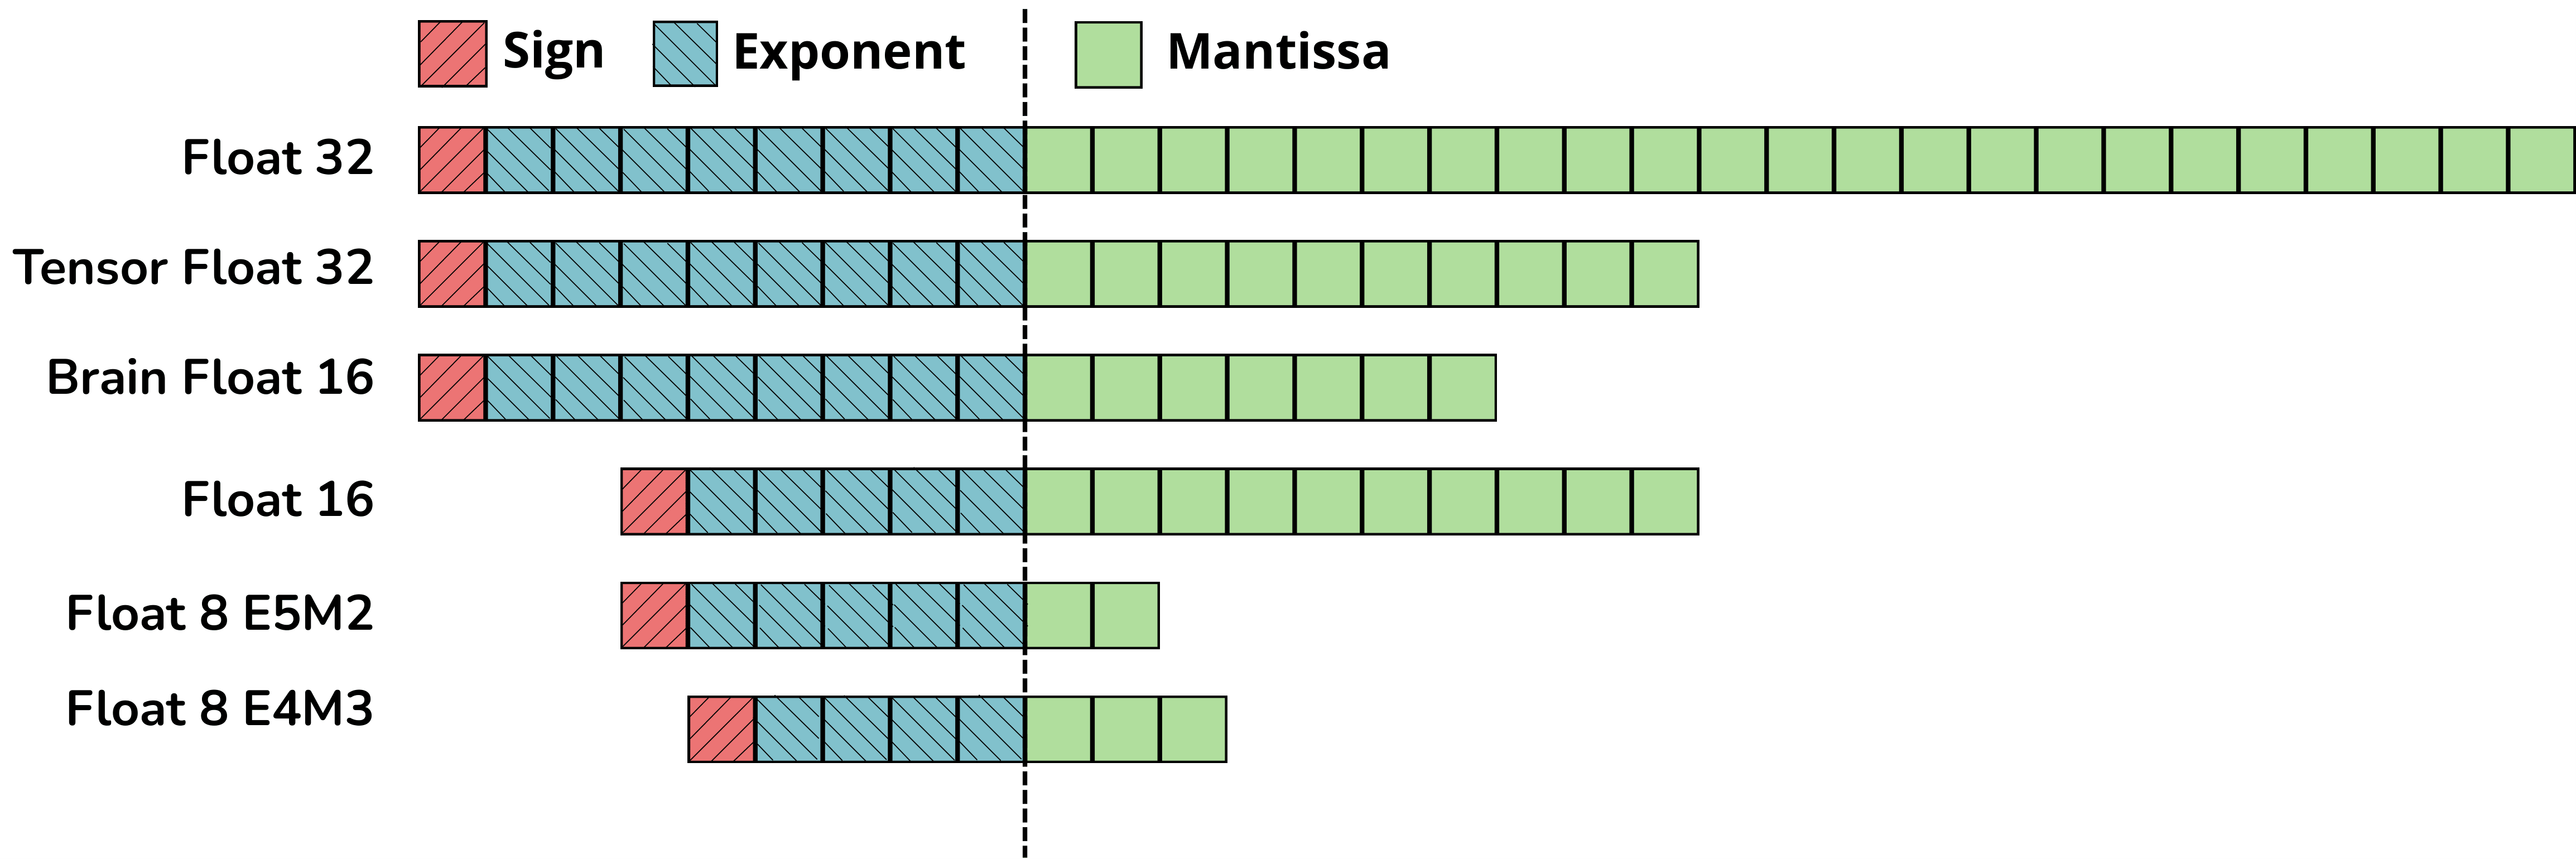
\includegraphics[width=\textwidth]{figs/Precision with hatch.pdf}
    \caption{Mixed Precision Floating-Point formats.}
    \tagpdfsetup{alttext={Mixed Precision Floating-Point formats.}}
    \label{fig:floating}
\end{figure}

Currently, two main types of FP8 quantization are used: W8A16 (8-bit weights and 16-bit activations) and W8A8 (8-bit weights and 8-bit activations). In particular, W8A8 typically employs the E4M3 format (4 exponent bits and 3 mantissa bits) for weights, and the E5M2 format (5 exponent bits and 2 mantissa bits) for activations. These two approaches target different hardware configurations. The former utilizes dedicated FP8 functional units to accelerate computation, while the latter is designed for hardware that only supports half-precision operations but still benefits from reduced memory usage.
Other quantization methods exist, but they fall outside the scope of this evaluation.

\subsection{Multi-GPU Inference}
\label{chap:background:sec:multigpu}

Growing model sizes and throughput requirements frequently exceed the memory and compute capacity of a single device, motivating multi-GPU strategies that distribute computation at the cost of increased communication. A variety of parallelism techniques have therefore been developed to balance memory capacity, communication overheads, and GPU utilisation.

\begin{figure}[h!]
    \centering
    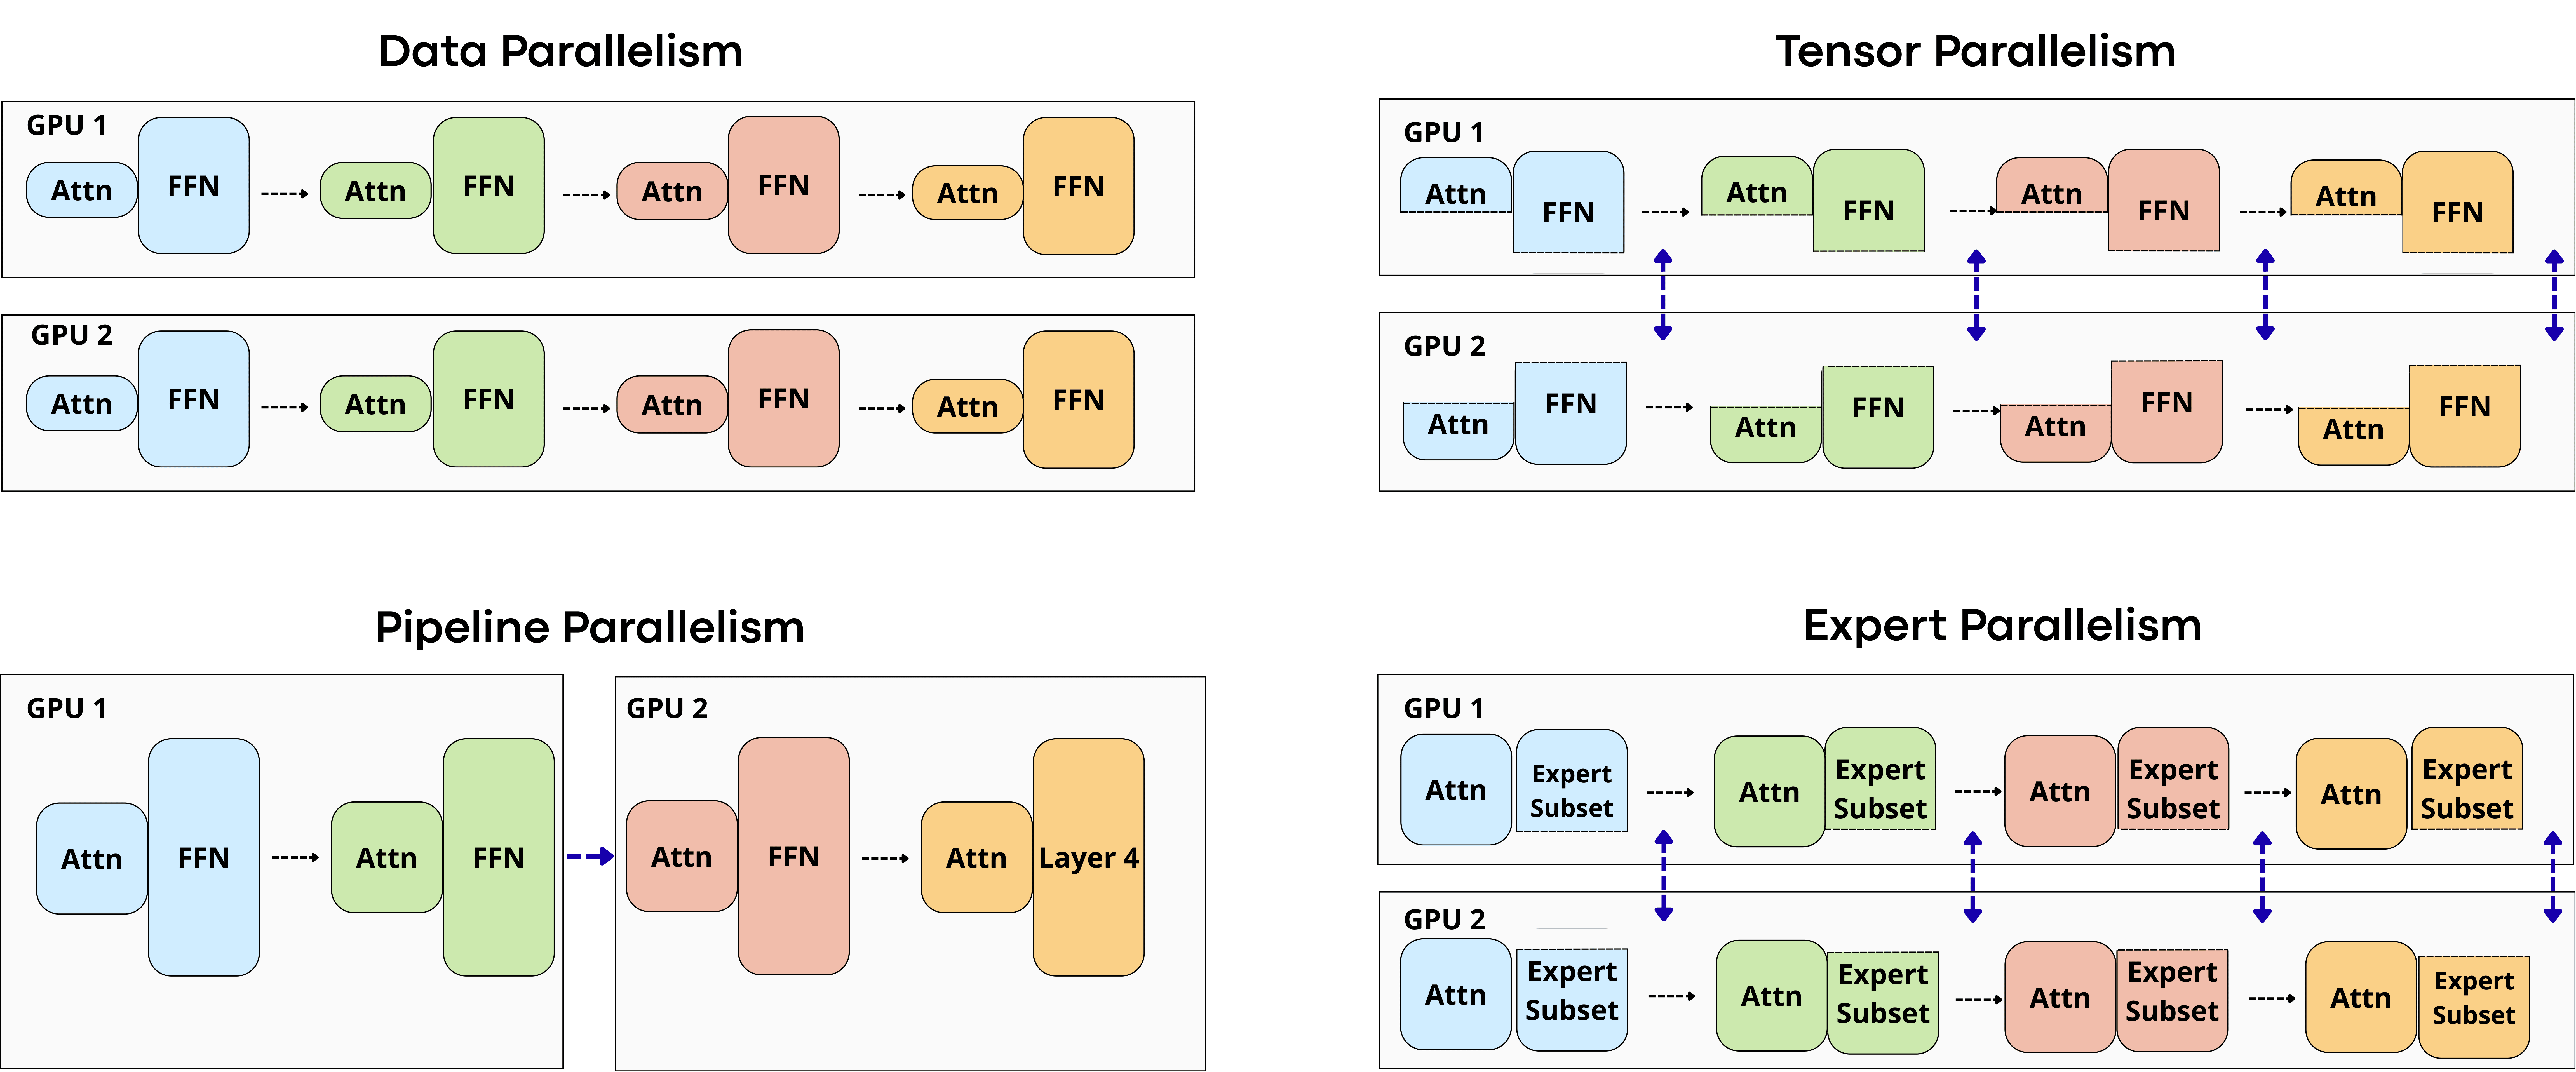
\includegraphics[width=0.95\textwidth]{figs/parallelism.pdf}
    \vspace{5mm}
    \caption{Comparison of multi-GPU techniques.}
    \tagpdfsetup{alttext={Comparison of multi-GPU techniques.}}
    \label{fig:parallel}
\end{figure}

\begin{itemize}
    \item \textbf{Data Parallelism (DP)} launches multiple independent model replicas on separate GPUs to increase serving throughput. Because each replica contains the full set of parameters, DP does not increase the effective memory available to a single model instance, but it scales well and requires no inter-GPU communication during inference.

    \item \textbf{Pipeline Parallelism (PP)} partitions the model’s layers across GPUs. Each device executes a contiguous block of layers and forwards intermediate activations to the next device. This expands the memory capacity accessible to a single model instance while introducing only moderate communication overhead.

    \item \textbf{Tensor Parallelism (TP)} shards parameters within each layer—such as attention heads and feed-forward weights—across multiple GPUs. This provides a finer-grained way to increase total available memory and keep all devices active, at the cost of frequent collective operations (e.g., all-gather).

    \item \textbf{Expert Parallelism (EP)} distributes the experts in Mixture-of-Experts layers across devices, allowing each GPU to store only a subset of expert parameters. Non-expert components—such as attention projections, layer norms, and routing modules—remain replicated on all devices. As a result, EP increases effective memory capacity primarily for expert-heavy layers while leaving the rest of the model duplicated.
\end{itemize}
\chapter{Background: Hardware Accelerators}
\label{chap:hardware}

LLM inference is a highly computational task dominated by large-scale matrix–matrix multiplications. This process poses three main challenges:
\begin{itemize}
    \item \textbf{Computation}: It requires executing a large number of floating-point operations.
    \item \textbf{Memory capacity}: It involves storing massive weight and activation matrices.
    \item \textbf{Memory bandwidth}: It demands frequent loading of large data volumes from memory.

\end{itemize}
For instance, performing a single forward pass of a 70-billion-parameter model in half precision (16-bit) entails approximately 140 BFLOPs of computation and 140 GB of memory reads.

To address these challenges, researchers have developed various parallel hardware accelerators that combine high memory bandwidth with large-scale parallel computing capabilities. Currently, Graphics Processing Units (GPUs) remain the dominant platform for LLM inference. However, Domain-Specific Architectures (DSAs) are emerging as promising alternatives, designed to provide greater efficiency for AI workloads \cite{chen2020survey, koilia2024hardware, silvano2025survey, kachris2025survey}.

This chapter provides a historical overview of the evolution of data center hardware accelerators used for AI inference, highlighting the key architectural trends shaping today’s computing landscape.

\section{Graphic Processing Units}
\label{chap:background:sec:gpu}

Graphics Processing Units (GPUs) are the most established class of accelerators for large-scale AI inference. They are designed around the \textbf{Single Instruction, Multiple Threads (SIMT) model}, which enables the parallel execution of thousands of lightweight threads. This parallelism makes GPUs highly efficient for the matrix and vector operations central to LLM inference. To support these operations, GPUs use a \textbf{multi-level memory hierarchy} that includes large off-chip DRAM for global storage and faster on-chip SRAM memories shared among thread blocks, ensuring high data throughput.

Modern General-Purpose GPUs (GPGPUs) emerged with NVIDIA’s Tesla architecture (2007) \cite{lindholm2008nvidia}, which transformed GPUs from fixed-function graphics devices into programmable, massively parallel processors. Tesla introduced uniform, fully programmable cores capable of dynamic workload balancing and non-graphics computations. Each GPU integrated 16 Streaming Multiprocessors (SMs), each containing 8 CUDA cores operating under the SIMT model. This architecture executed instructions in groups of 32 threads, known as warps, achieving SIMD-like efficiency while allowing limited control-flow divergence.

Tesla also established the standard GPU memory hierarchy still in use today—comprising per-thread \textbf{local memory}, per-SM \textbf{shared memory}, and \textbf{global DRAM}—along with L1 caches per SM and a unified L2 cache for improved data locality. Complementing this hardware innovation, NVIDIA introduced the \textbf{CUDA} programming model, a C/C++ extension that provides APIs for CPU–GPU coordination, memory management, and thread scheduling. CUDA laid the foundation for general-purpose GPU computing, enabling efficient deployment of parallel workloads such as deep learning inference.

This section presents the architecture of the most relevant data center–level GPUs developed by NVIDIA, AMD, and Intel, highlighting their evolution and design principles for AI inference workloads.

\subsection{NVIDIA GPUs}

Modern NVIDIA AI-oriented GPUs fall in the category of Tensor-Core GPUs. Their distinctive features are the presence of high-speed off-chip HBM memories, as opposed to standard DRAM, and the Tensor Cores, which accelerate matrix-matrix multiplications in mixed precision.
The NVIDIA P100 was the first to feature HBM memory, while the \textbf{NVIDIA Volta V100} \cite{choquette2018volta} first introduced Tensor Cores, representing a pivotal point in AI hardware.
In the remainder of this section, we provide a detailed discussion of the architectures of the NVIDIA V100, A100, and H100.

The \textbf{Nvidia Volta V100} is composed of six GPU Processing Clusters (GPCs) and features a total of 80 Streaming Multiprocessors (SMs). Each SM has four processing blocks, each featuring dedicated cores for single- and double-precision floating-point numbers and integer types. They also feature a Special Functional Unit (SFU) and two \textbf{Tensor Cores}: a dedicated functional unit that performs a matrix-matrix multiplication and accumulation.
Another major novelty is the unification of the L1 cache and the shared memory. According to the application's needs, the programmer can utilize up to 96 KB of the 128 KB L1 cache as shared memory, reserving the remaining space for caching.
The chip also offers 6MB of L2 cache, shared by all the GPCs, that acts as an intermediary between the SMs and the off-chip memory, consisting of 16 GB of HBM2 that operates at 0.90 TB/s.

The \textbf{NVIDIA Ampere A100} \cite{Choquette2021} represents a significant advancement over its predecessor, introducing numerous innovations and improvements.
It features 108 Streaming Multiprocessors, each divided into four processing blocks containing double-, single-, and integer-precision units, as well as third-generation Tensor Cores.
Unlike first-generation Tensor Cores, which are limited to FP16, the A100 cores support multiple data types (see \ref{tab:gpus}) and include fine-grained sparsity optimization, which doubles the throughput of sparse matrices. The \textbf{TF32} format is notable for combining the 8-bit exponent of FP32 with the 10-bit mantissa of FP16, offering a balance between precision and efficiency. The A100 also improves data delivery to the Tensor Cores by introducing asynchronous copy operations.
To support larger models, the size of memory is significantly increased: the L2 cache is increased to 40 MB, and the VRAM is either 40 or 80 GB of HBM2. There is also an improvement of $2.3\times$ in L2 cache throughput and $1.7\times$ in HBM throughput. Additionally, the A100 offers an in-hardware data compression feature that improves bandwidth by up to $4\times$.
The A100 also introduces two notable novelties: the third-generation NVLink and the Multi-Instance GPU (MIG) feature, which enables support for up to seven independent virtual GPUs on the same physical GPU.

The \textbf{NVIDIA Hopper H100} \cite{Choquette2023} represents an ulterior step forward with respect to the NVIDIA Ampere A100, featuring 132 redesigned Streaming Multiprocessors. Each multiprocessor comprises four processing blocks that integrate double-, single-precision, and integer units, as well as a fourth-generation Tensor Core.
The renewed Tensor Cores support improves throughput compared to the predecessor and adds support for 8-bit floating-point (\textbf{FP8}) precision (see \ref{fig:floating}).
The memory is improved by upgrading the off-chip DRAM to HBM3 and by increasing the sizes of the L1 and L2 caches.
To improve data locality, the Hopper architecture adds a new level in the CUDA hierarchy: the \textbf{thread block cluster}, which sits between the thread blocks and the grid and consists of up to 16 thread blocks. The cluster can benefit from improved data locality thanks to the new SM-to-SM communication network, which allows SMs to access the shared memory of other Streaming Multiprocessors and synchronize on barriers distributed across shared memory.
The Hopper Architecture also offers the fourth generation of NVLink and new types of barriers that facilitate asynchronous execution of threads and asynchronous data transfers.

Together with Hopper, NVIDIA also introduced \textbf{Grace}, a CPU featuring 72 Arm v9.0 cores explicitly designed to be paired with a GPU on a CPU-GPU System on a Chip (SoC). 
The \textbf{Grace-Hopper GH200} features a Grace CPU and a Hopper H100 GPU interconnected by a 900 GB/s cache coherent interconnection (NVLink-C2C). In total, the SoC has 96 GB of HMB memory and 512 GB of LPDDR5X DRAM. All the memory can be directly accessed by both processors, as they share the same system-wide page table.

\subsection{AMD GPUs}

In 2017, AMD introduced the Instinct MI series, derived from the Vega architecture and designed for scientific computing and AI workloads. In 2020, AMD separated its GPU lineup into RDNA for graphics and CDNA for data center computing, with CDNA architectures removing rendering features and adding dedicated matrix-multiply units similar to NVIDIA’s Tensor Cores. As noted by AMD researchers \cite{Loh2023}\cite{Smith2024}, CDNA designs are closely linked to the AMD EHP concepts developed under the U.S. Department of Energy’s Exascale Computing Program, representing early steps toward exascale-ready CPU–GPU systems.

The \textbf{AMD Instinct MI100} is the first CDNA GPU.
It features 120 Compute Units (CU) organized in four arrays. CUs feature both scalar and vector capabilities, thanks to dedicated register files, execution units, and cache for both scalar and vector operations. Vector execution units execute 64-wide wavefronts (similar to NVIDIA warps) over four cycles, thanks to a 16-wide SIMD vector pipeline that operates on both single- and double-precision data types.
The novelty of CDNA CUs lies in the introduction of Matrix Fused Multiply-Add (MFMA) units, which, similar to NVIDIA Tensor Cores, perform matrix-matrix multiplications.
The memory hierarchy of CDNA consists of the scalar and vector data caches of CUs, an 8 MB L2 cache shared by all CUs, and 32 GB of off-chip HMB2 memory that operates at 1.23 TB/s.
The MI100 is also the first card to feature AMD's Infinity Fabric technology, which enables inter-GPU communication similar to NVIDIA's NVLink.

\textbf{AMD CNDA 2:} The second generation of AMD CDNA cards represents an important step forward in AMD's GPU design.
The basic building block of CDNA 2 GPUs is called the Graphics Compute Die (GCD). Each GCD features four arrays of 28 compute units, totaling 112 (with 104 active in the MI210 and MI250, and 110 active in the MI250X). CDNA 2 introduces the concept of \textbf{multi-die GPUs}, significantly enhancing computational power. While the MI210 features a single GCD, the MI250 and MI250X are equipped with two GCDs, effectively doubling both the computational performance and memory capacity within a single board.
The Compute Units feature includes scalar, vector, and matrix cores. Vector cores operate on 64-wide wavefronts with 16-wide pipelines, supporting both single- and double-precision data types. Compared to its predecessor, the CDNA 2 Compute Units improve double-precision performance by a factor of two and support the new packed floating-point data type, enabling faster throughput for floating-point operations. Additionally, the matrix units undergo significant improvements, improving throughput and adding support for double-precision matrices.
Regarding memory, each GCD features 8 MB of L2 cache and 64 GB of HBM2e memory (1.6 TB/s).
A major innovation of CDNA 2 is the adoption of an innovative caching system that enables a unique memory addressing space for both the CPU and GPU, simulating an APU system where no CPU-GPU data transfers are necessary. 

\textbf{AMD CNDA 3:} The third generation of CDNA cards adopts an even more advanced approach to dense integration than CDNA 2, combining multiple dies within a single chip. This design realizes the 12-year-old AMD vision of a heterogeneous APU\cite{Smith2024}, incorporating both CPUs and GPUs on the same chip. The  DNA 3 family features two cards: the MI300X and the MI300A. The MI300X features eight accelerator complex dies (XCDs), similar to CDNA 2 GCDs, while the MI300A features six XCDs and three CPU complex dies (CCDs). 
The XCD features 40 CUs (38 active) and a set of shared resources, including the scheduler and four Asynchronous Compute Engines (ACE) that assign computing tasks to the Compute Units (CUs). The CUs also share 4 MB of L2 cache and have 32 KB of L1 cache each.
The biggest improvement compared to the previous generation is in the Matrix Cores, which offer improved performance compared to the previous generation and support new data types (Tensor Float and FP8).
Another important difference from the previous generation is the introduction of a new level of cache called Infinity cache, which sits between the off-chip memory and the on-chip L2 cache. The off-chip memory also underwent significant improvement, offering 128 GB of HMB3 memory (5.3 TB/s) on the MI300A and 192 GB on the MI300X. Similar to CDNA 2, CDNA 3 provides a unique memory addressing space shared by the CPU and the GPU, with the notable difference that in the MI300A APU, the memory is not only logically but also physically shared between the CPU and the GPU.

\subsection{Intel GPUs}

The Intel Xe GPU lineup, formerly known as Intel Ponte Vecchio \cite{gomes2022ponte}, comprises three models: the Intel Max 1100, Intel Max 1350, and Intel Max 1550. The latter powers the Aurora Supercomputer.

The \textbf{Intel Max 1550} is a multi-tile GPU featuring two Xe-stacks. Each Xe-stack contains four Xe-slices, providing a total of 64 Xe-cores, 64 ray-tracing units, and one media engine. Every Xe-core integrates eight vector engines (512-bit wide) and eight matrix engines (4096-bit wide). The vector engines support FP16, FP32, and FP64 data formats, while the matrix engines handle int8, FP16, and bfloat16 precisions.

In terms of memory, each Xe-core includes 512 KB of SRAM, which functions as shared memory or L1 cache. Each Xe-stack also incorporates 204 MB of shared L2 cache.

\ref{tab:gpus} summarizes all the architectural features of the modern AI GPUs discussed in this section.

\begin{table}[h!]
\centering
\footnotesize
\caption{Datacenter-level GPUs from Nvidia, AMD, and Intel.}
\label{tab:gpus}

\begin{tabularx}{\textwidth}{l l c c c c c c}
\toprule
\textbf{Vendor} & \textbf{Name} & \textbf{Year} & \textbf{Cores} & \textbf{TFLOPS} & \textbf{Cache} & \textbf{RAM} & \textbf{TDP} \\
\midrule

\textbf{NVIDIA}
& \textbf{V100}  & 2017 & 80 SM  & \makecell[l]{TF32: 125} 
& \makecell[l]{L1: 128 KB \\ L2: 16 MB} 
& \makecell[l]{HBM2: 32 GB \\ 0.90 TB/s} 
& 400 W \\

\textbf{NVIDIA}
& \textbf{A100}  & 2020 & 108 SM 
& \makecell[l]{TF32: 156 \\ FP16: 312} 
& \makecell[l]{L1: 164 KB \\ L2: 40 MB} 
& \makecell[l]{HBM2e: 80 GB \\ 2.03 TB/s} 
& 400 W \\

\textbf{NVIDIA}
& \textbf{H100}  & 2022 & 132 SM 
& \makecell[l]{TF32: 989 \\ FP16: 1979 \\ FP8: 3958} 
& \makecell[l]{L1: 256 KB \\ L2: 50 MB} 
& \makecell[l]{HBM3: 80 GB \\ 3.35 TB/s} 
& 700 W \\

\textbf{NVIDIA}
& \textbf{GH200} & 2023 & 132 SM 
& \makecell[l]{TF32: 989 \\ FP16: 1979 \\ FP8: 3958} 
& \makecell[l]{L1: 256 KB \\ L2: 50 MB} 
& \makecell[l]{HBM3: 96 GB \\ 3.9 TB/s} 
& 450 W \\

\midrule

\textbf{AMD}
& \textbf{MI100}  & 2020 & 120 CU 
& \makecell[l]{FP32: 23 \\ FP16: 185} 
& \makecell[l]{L1: 16 KB \\ L2: 8 MB} 
& \makecell[l]{HBM2e: 32 GB \\ 1.2 TB/s} 
& 560 W \\

\textbf{AMD}
& \textbf{MI250}  & 2021 & 220 CU 
& \makecell[l]{FP32: 90 \\ FP16: 362} 
& \makecell[l]{L1: 16 KB \\ L2: 16 MB} 
& \makecell[l]{HBM2e: 128 GB \\ 3.2 TB/s} 
& 500 W \\

\textbf{AMD}
& \textbf{MI300X} & 2023 & 304 CU 
& \makecell[l]{TF32: 654 \\ FP16: 1307 \\ FP8: 2615} 
& \makecell[l]{L1: 32 KB \\ L2: 4 MB \\ L3: 256 MB} 
& \makecell[l]{HBM3: 192 GB \\ 5.3 TB/s} 
& 750 W \\

\textbf{AMD}
& \textbf{MI300A} & 2023 & 228 CU 
& \makecell[l]{TF32: 490 \\ FP16: 980 \\ FP8: 1961} 
& \makecell[l]{L1: 32 KB \\ L2: 4 MB \\ L3: 256 MB} 
& \makecell[l]{HBM3: 128 GB \\ 5.3 TB/s} 
& 760 W \\

\midrule

\textbf{Intel}
& \textbf{MAX 1550} & 2023 & 128 Xe 
& \makecell[l]{FP16: 832} 
& \makecell[l]{L1: 64 KB \\ L2: 408 MB} 
& \makecell[l]{HBM2e: 128 GB \\ 3.28 TB/s} 
& 600 W \\

\bottomrule
\end{tabularx}
\end{table}

\subsection{GPU limitations: the memory wall}

As discussed earlier, Graphics Processing Units (GPUs) are the most widespread type of hardware accelerator for LLM inference. Their success stems from their ability to perform massive numbers of floating-point operations in parallel, which is essential for deep neural network (DNN) training and inference. By scaling out the number of cores, GPUs have sustained performance growth despite the slowdown in transistor miniaturization and the onset of dark silicon.

However, GPUs often fail to reach their theoretical peak throughput during large language model (LLM) inference because these workloads are typically \textit{memory-bound}. As shown in Table~\ref{tab:gpus}, GPU compute throughput (in FLOPS) exceeds memory bandwidth by up to two orders of magnitude, meaning that data transfer between memory and compute units dominates latency and limits overall performance.

Gholami et al.~\cite{gholami2024ai} highlight that this imbalance is widening over time. While floating-point performance has increased by a factor of three every two years, memory bandwidth has increased by only about 1.6 times per year.
This growing disparity between computation and data movement is known as the \textbf{memory wall}~\cite{gholami2024ai}.

To mitigate this limitation, researchers have developed \textit{Domain-Specific Architectures (DSAs)} designed to minimize data transfer during DNN inference and training~\cite{Hooker2021, Dean2018}. The first prominent example was Google’s \textbf{Tensor Processing Unit (TPU)}~\cite{Jouppi2017}, which demonstrated how customized architectures can achieve substantial gains in both speed and energy efficiency.

\newpage
\section{AI Accelerators - TPUs}\label{chap:background:sec:tpu}

This section describes the design \textbf{Tensor Processing Units (TPU)} and other architectures that share common features. \ref{tab:tpus} summarises the main features of the architectures discussed in this section, namely Google TPUs, Habana Lab TPCs, and Groq LPus.

\begin{table}[h!]
\centering
\footnotesize
\caption{Tensor-Core based accelerators from Google, Habana Labs, and Groq.}
\label{tab:tpus}

\begin{tabularx}{\textwidth}{l l c c c c c c}
\toprule
\textbf{Vendor} & \textbf{Name} & \textbf{Year} & \textbf{Cores} & \textbf{Data Types} & \textbf{On-chip} & \textbf{Off-chip} & \textbf{TDP} \\
\midrule

\textbf{Google}
& \textbf{TPU v1}  & 2015 & \makecell[l]{1 core \\ 1 MXU/core} & int8 
& 28 MB & DDR3: 8 GB & 75 W \\

\textbf{Google}
& \textbf{TPU v2}  & 2017 & \makecell[l]{2 cores \\ 1 MXU/core} & BF16 
& 32 MB & HBM: 16 GB & 280 W \\

\textbf{Google}
& \textbf{TPU v3}  & 2018 & \makecell[l]{2 cores \\ 2 MXU/core} & BF16 
& 32 MB & HBM: 32 GB & 450 W \\

\textbf{Google}
& \textbf{TPU v4}  & 2021 & \makecell[l]{2 cores \\ 4 MXU/core} & BF16, int8 
& 32 MB & HBM: 32 GB & N/A \\

\textbf{Google}
& \textbf{TPU v4i} & 2021 & \makecell[l]{1 core \\ 4 MXU/core} & BF16, int8 
& 144 MB & HBM: 32 GB & 175 W \\

\textbf{Google}
& \textbf{TPU v5e} & 2023 & \makecell[l]{1 core \\ 4 MXU/core} & BF16, int8 
& 112 MB & HBM: 16 GB & N/A \\

\textbf{Google}
& \textbf{TPU v5p} & 2023 & \makecell[l]{2 cores \\ 4 MXU/core} & BF16, int8 
& 48 MB & HBM: 95 GB & N/A \\

\textbf{Google}
& \textbf{TPU v6e} & 2024 & \makecell[l]{1 core \\ 4 MXU/core} & BF16, int8 
& N/A & HBM: 32 GB & N/A \\

\textbf{Google}
& \textbf{TPU v7p} & 2025 & N/A & BF16, FP8 
& N/A & HBM: 192 GB & N/A \\

\midrule

\textbf{Habana}
& \textbf{Goya}    & 2018 & \makecell[l]{8 TPC \\ 1 MME} 
& int8 
& 28 MB & DDR4: 16 GB & N/A \\

\textbf{Habana}
& \textbf{Gaudi}   & 2019 & \makecell[l]{8 TPC \\ 1 MME} 
& FP32, int8 
& 24 MB & HBM2: 32 GB & N/A \\

\textbf{Habana}
& \textbf{Gaudi 2} & 2022 & \makecell[l]{24 TPC \\ 2 MME} 
& \makecell[l]{FP32, BF16 \\ FP16, FP8} 
& 48 MB & HBM: 96 GB & 600 W \\

\textbf{Habana}
& \textbf{Gaudi 3} & 2024 & \makecell[l]{64 TPC \\ 8 MME} 
& \makecell[l]{FP32, TF32 \\ FP16, BF16, FP8} 
& 96 MB & HBM: 128 GB & 900 W \\

\midrule

\textbf{Groq}
& \textbf{GroqCard} & 2019 & 320 lanes 
& \makecell[l]{int8, int16 \\ FP16} 
& 230 MB & -- & 275 W \\

\bottomrule
\end{tabularx}
\end{table}

\subsection{Google TPU}
\label{chap:background:sec:tpu}

In 2013, Google began developing the \textbf{Tensor Processing Unit (TPU)}, the first domain-specific accelerator for neural network inference. At that time, CPUs were used for inference and GPUs for training, but this approach was both costly and energy-intensive. To address this, Google designed a single-core, domain-specific processor centred on a \textbf{Matrix Multiply Unit (MXU)}, a systolic array specialised for dense matrix multiplications. This architecture minimized energy-hungry memory accesses and control operations through spatial computation~\cite{jouppi2018motivation}, achieving order-of-magnitude improvements in efficiency and marking the start of domain-specific architectures for AI.

Several TPU generations (v1–v7) have since been released, summarised in Table~\ref{tab:tpus}. The main architectural features of the first four generations—those publicly documented—are outlined below.

\textbf{TPU v1}~\cite{Jouppi2017} was a PCIe-attached co-processor optimized for inference. Its core component, the 256×256 \textbf{MXU}, consisted of 65,536 int8 multipliers operating in a systolic array that streamed data directly between adjacent cells. Each cycle produced 256 partial sums, accumulated in on-chip registers. The chip included 24~MB of on-chip SRAM (the Unified Buffer) for activations and 8~GB of off-chip DDR3 DRAM for weights. A Very Long Instruction Word (VLIW) control unit allowed the compiler to statically schedule parallel operations, simplifying control logic while maintaining high utilisation.

\textbf{TPU v2 and v3}~\cite{Norrie2021} extended the design for training workloads, introducing \textbf{bfloat16} arithmetic to replace int8 quantisation, providing a balance between precision and hardware cost. Each core integrated a scalar unit, vector unit, and MXU arranged in a push–pop pipeline, where the MXU acted as a co-processor for the vector unit. Memory organisation was restructured into a unified \textbf{Vector Memory} scratchpad, while off-chip DDR was replaced by 16~GB of \textbf{HBM}, boosting bandwidth by over 20×. TPU v2 adopted a dual-core layout with a 2D torus interconnect for large-scale scaling. TPU v3 doubled the MXUs per core, increased clock speed, expanded HBM capacity, and improved inter-chip bandwidth, enabling significantly higher throughput for large models.

\textbf{TPU v4i}~\cite{Jouppi2021}, introduced in 2021, was designed as an inference-oriented counterpart to the training-focused TPU v4. It retained the systolic array architecture but incorporated four MXUs per core for increased parallelism. The memory hierarchy added a new 128~MB \textbf{Common Memory (CMEM)} layer between on-chip vector memory and off-chip HBM, reducing data transfer overhead. TPU v4i supported both int8 and bfloat16 data types, reflecting the industry trend toward higher precision inference. Like previous versions, it used HBM to sustain high bandwidth and employed dedicated SRAM regions for scalar values and instructions.

\textbf{TPU v5–v7} continue this evolution, though details are mostly undisclosed. The fifth generation includes two variants: \textbf{TPU v5p} (performance-optimised) and \textbf{TPU v5e} (cost-efficient), both with four MXUs per core and support for int8 and bfloat16. The sixth-generation \textbf{TPU v6e (Trillium)} doubles memory capacity and introduces 256×256 MXUs per core, while the forthcoming \textbf{TPU v7p (Ironwood)} further increases memory (192~GB) and adds support for 8-bit floating-point formats, signalling a shift toward finer precision–efficiency trade-offs in inference hardware.

\subsection{Habana Labs TPC}
\label{chap:background:sec:habana}

Founded in 2016 and acquired by Intel in 2019, \textbf{Habana Labs} introduced the \textbf{Tensor Processing Core (TPC)} architecture in 2018, a family of domain-specific AI accelerators for inference and training. Similar to Google’s TPUs, Habana’s design centres on specialised matrix multiplication engines integrated with programmable compute cores. The company’s main lineup includes the inference accelerators \textbf{Goya} (2018) and \textbf{Greco} (2022), and the training accelerators \textbf{Gaudi} (2019), \textbf{Gaudi2} (2022), and \textbf{Gaudi3} (2024).

\textbf{Habana Goya}~\cite{Gwennap2019} was the first inference processor, featuring an HL-1000 chip with eight \textbf{TPCs}, one \textbf{Matrix Multiplication Engine (MME)}, and a hierarchical memory system. Each TPC is a VLIW SIMD processor supporting integer and floating-point operations (8–32 bits). The MME is a 256×256 systolic array for int8 matrix multiplication shared across all TPCs. Goya uses 16 GB DDR4 memory and on-chip SRAM, optimised for low-latency, energy-efficient inference.

\textbf{Habana Gaudi}~\cite{Gwennap2019} adapted Goya for training, adding floating-point GEMM support, 32~GB of high-bandwidth \textbf{HBM2} memory, and ten 100~Gb/s Ethernet links for direct chip-to-chip communication, enabling distributed training without host coordination.

\textbf{Habana Gaudi2}~\cite{gaudi2} significantly scaled the architecture, tripling TPCs (8→24) and HBM capacity (6×16~GB HBM2E). It also expanded interconnect bandwidth with 24 100-Gb/s Ethernet ports and introduced mixed-precision support—\textbf{FP32}, \textbf{bfloat16}, \textbf{FP16}, and \textbf{FP8} — across both TPCs and GEMM units. Dedicated decoding engines were added for handling compressed image and video data.

\textbf{Habana Gaudi3}~\cite{Kaplan2024} further scaled the design to four clusters, each with 16 TPCs and two MMEs, totalling 96 TPCs and eight GEMM units. On-chip memory was expanded from 48~MB SRAM to a 96~MB L2 cache, while external memory grew to eight 16~GB HBM2E stacks, offering higher parallelism, bandwidth, and scalability for large AI workloads.

\subsection{Groq LPU}

The Groq Language Processing Unit (LPU) \cite{Gwennap, Abts2022} is a dataflow accelerator introduced in 2019 by Groq.
The LPU is built as a systolic array of heterogeneous functional units where data flows horizontally through lanes and instructions vertically across them. Sixteen lanes form a superlane, and the LPU contains 20 active superlanes plus one redundant lane. Each superlane processes streaming data through a Vector Unit, Memory Unit, Switch Unit, and Matrix Unit arranged symmetrically into eastward and westward hemispheres. The Vector Unit has 16 ALUs supporting integer–floating-point conversions and activation functions. The Memory Unit provides 44 slices of 128 kB SRAM (5.5 MB total) with up to two reads and writes per cycle for instructions and activations. The Switch Unit handles tensor reshaping, while the Matrix Unit includes 320 MACs per lane optimised for int8 but also supporting int16 and FP16. So, in total, each superlane features 20 $16\times 16$ matrix-matrix multiplication units.

Groq LPU design resembles Google's TPU as it includes vector and matrix-matrix multiplication functional units optimised for integer operations. On the other hand, the way instructions are pipelined through the lanes is drastically different from Google's design. Another key difference is the absence of DRAM memory and caches, which allows the LPU to achieve full determinism, allowing its compiler to statically schedule every operation with cycle-accurate predictability.

\section{AI Accelerators - Dataflow}\label{chap:background:sec:dflow}

This section describes the second class of Domain-Specific Accelerators for LLM inference, which consists of \textbf{dataflow accelerators}. \ref{tab:dflow} summarizes the main features of the architectures discussed in this section, namely SambaNova RDAs, Cerebras WSE, and GraphCore IPUs.

\subsection{SambaNova RDA}
\label{chap:background:sec:sambanova}

Founded in 2017, \textbf{SambaNova Systems} develops dataflow accelerators for DNN training and inference, inspired by the \textbf{Plasticine} prototype architecture~\cite{Prabhakar2017}.

\textbf{Plasticine} is a coarse-grained reconfigurable architecture (CGRA) that exploits spatial parallelism for compute patterns such as map and reduce. Unlike bit-level FPGAs, CGRAs use word-level processing elements (ALUs, DSPs) connected through structured interconnects, achieving higher density and clock speeds. Plasticine consists of \textbf{Pattern Compute Units (PCUs)} and \textbf{Pattern Memory Units (PMUs)} arranged in a grid, managed by hierarchical controllers that coordinate pipelined and streaming execution. Address Generators and Coalescing Units handle off-chip memory, optimizing access patterns and reducing traffic.

Building on this concept, SambaNova’s \textbf{Reconfigurable Dataflow Architecture} \cite{sambanova} combines tiled PCUs and PMUs linked by a high-bandwidth switch fabric, with AGUs and CUs managing external memory. Its software stack, \textbf{SambaFlow}, integrates with PyTorch and TensorFlow, automatically mapping models to hardware. A Dataflow Graph Analyzer identifies dependencies, while the compiler optimizes execution through parallelization and pipelining. RDA also supports concurrent workloads, allowing simultaneous preprocessing, training, and inference tasks.

The first generation, the \textbf{Cardinal SN10-8R}, featured eight RDUs, each with 640 PCUs and PMUs, and up to 12~TB of configurable DRAM. Its successor, \textbf{Cardinal SN30-8R}, increased compute density to 1,284 PCUs and PMUs per RDU, with 640~MB on-chip memory and 1~TB of DRAM per device. The 2024 \textbf{SN40L-16}~\cite{Prabhakar2024}, optimized for LLM inference, integrates 16 RDUs with 1,040 PCUs and PMUs each, 520~MB of SRAM, and hybrid memory combining 64~GB HBM with 768~GB DDR—significantly boosting bandwidth for compute-bound workloads.


\subsection{Cerebras WSE}
\label{chap:background:sec:cerebras}

Founded in 2015, \textbf{Cerebras Systems} develops large-scale AI accelerators for DNN training and inference. The company has released three systems: the \textbf{CS-1} (2019) with \textbf{WSE-1}, the \textbf{CS-2} (2021) with \textbf{WSE-2}, and the \textbf{CS-3} (2024) featuring \textbf{WSE-3}.

The \textbf{Wafer-Scale Engine (WSE)} is the first processor built on a full 300~mm silicon wafer (462.25~cm$^2$), hosting 400{,}000 cores in WSE-1, 850{,}000 in WSE-2, and 900{,}000 in WSE-3. Each core is a general-purpose compute element supporting arithmetic, logic, and tensor operations through hardware state machines and \textbf{Data Structure Registers (DSRs)} that manage tensor metadata. The 64-bit datapath includes four fused FPMAC units operating on FP16 and bfloat16 data for high tensor throughput.

The WSE adopts a fully distributed memory architecture to maximize locality and bandwidth. Each core integrates 48~KB of SRAM, yielding 44~GB of total on-chip memory in WSE-3. Cores communicate through a 2D mesh of routers, allowing weights and activations to stream efficiently across the wafer and to external \textbf{MemoryX} units, removing the need for shared DRAM or intermediate buffers.

Computation follows a dataflow execution model where operations are triggered by data arrival rather than instruction sequencing. This enables fine-grained sparsity filtering and high energy efficiency. Each core supports dynamic scheduling with up to eight concurrent micro-threads, selecting ready operations based on data availability and priority to improve utilization and reduce latency.


\subsection{Graphcore IPU}
The \textbf{Intelligent Processing Unit (IPU)} by Graphcore is a dataflow-based accelerator designed for AI workloads. Two generations exist: the \textbf{Colossus MK1} (2017) with GC2 IPUs and the \textbf{Colossus MK2} (2020) with GC200 IPUs.

The IPU implements a true \textbf{MIMD} architecture following the \textbf{Bulk Synchronous Parallel (BSP)} model~\cite{Jia2019}, which structures computation into three stages: local execution on private memory, inter-tile communication, and global synchronization. Computation occurs on independent \textbf{tiles}, each with its own processor, local SRAM, and an \textbf{Accumulating Matrix Product (AMP)} unit optimized for matrix multiplications and convolutions. Tiles support up to six threads via SMT, with 1,216 cores (7,296 threads) in the first generation and 1,472 cores (8,832 threads) in the second. Each AMP unit performs up to 16~FP32 or 64~FP16 operations per cycle.

Tiles operate exclusively on local memory—256~KB in the GC2 and 624~KB in the GC200—eliminating caches and shared DRAM while ensuring deterministic performance. Inter-tile communication is handled by the on-chip \textbf{IPU Exchange} and off-chip \textbf{IPU Links}, enabling large-scale, multi-IPU systems.

Programming is performed using the \textbf{Poplar SDK}, where models are represented as computation graphs. The compiler maps graph vertices to threads and edges to communication paths, automatically managing the compute, communication, and synchronization phases under the BSP model.

\begin{table}[h!]
\centering
\footnotesize
\caption{Datacenter-level dataflow AI accelerators from SambaNova, Cerebras, and Graphcore.}
\label{tab:dflow}

\begin{tabularx}{\textwidth}{l l c c c c c c}
\toprule
\textbf{Vendor} & \textbf{Name} & \textbf{Year} & \textbf{Cores} & 
\textbf{TFLOPS} & \textbf{On-chip} & \textbf{Off-chip} & \textbf{TDP} \\
\midrule

\textbf{Graphcore}
& GC2   & 2017 & 1,216 & FP16: 125 
& 300 MB 
& -- 
& 150 W \\

\textbf{Graphcore}
& GC200 & 2020 & 1,472 & FP16: 250 
& 900 MB 
& -- 
& 300 W \\

\midrule

\textbf{SambaNova}
& SN10  & 2021 & 640 
& BF16: N/A 
& 300 MB 
& DRAM: 1.5 TB 
& N/A \\

\textbf{SambaNova}
& SN30  & 2022 & 1,284 
& BF16: 660 
& 640 MB 
& DRAM: 1 TB 
& N/A \\

\textbf{SambaNova}
& SN40L & 2023 & 1,040 
& BF16: 638 
& 520 MB 
& \makecell[l]{HBM: 64 GB \\ DRAM: 768 GB} 
& 900 W \\

\midrule

\textbf{Cerebras}
& CS2 (WSE2) & 2021 & 850K 
& BF16: N/A 
& 41 GB 
& MemoryX 
& 23 kW \\

\textbf{Cerebras}
& CS3 (WSE3) & 2024 & 900K 
& BF16: 125K 
& 44 GB 
& MemoryX 
& 23 kW \\

\bottomrule
\end{tabularx}
\end{table}
\chapter{Methodology}
\label{chap:methods}

With this thesis, we aim to measure and compare the LLM inference performance and energy efficiency of a diverse set of accelerated servers across multiple deployment scenarios. However, the heterogeneity of models, hardware, and software stacks, as well as the numerous interacting factors that influence performance, makes this task non-trivial. To structure our analysis, we begin by identifying the principal factors that impact LLM inference performance, focusing on four key elements:

\begin{itemize}
\item \textbf{Sequence length}: the number of input and output tokens generated. We ensure consistency by using the same inference dataset (Section \ref{chap:methods:sec:dataset}) for all experiments.
\item \textbf{Model architecture}: the characteristics of the LLM being served. We address the heterogeneity of LLM models by evaluating a diverse set of popular open-source models and examining their characteristics in relation to performance. In particular, we analyze:
\begin{itemize}
\item \textbf{Model Size}: the total number of model parameters;
\item \textbf{Sparsity}: the proportion of parameters that are sparsely activated, in the case of Mixture-of-Experts (MoE) models.
\item \textbf{Quantization}: the numerical format used for model weights and activations. Wherever supported, we compare 16-bit precision with 8-bit precision.
\end{itemize}
\item \textbf{Parallelism}: The number of sequences processed in parallel (\textbf{batch size}) and the number of devices used for inference greatly impact performance, depending on the parallel serving strategy chosen (\textbf{Data, Pipeline, Tensor or Expert Parallelism}).
\item \textbf{Inference Engine}: the software stack influences performance. We maintain consistency by using the same inference engine (vLLM \cite{kwon2023efficient}) across all the GPU servers. Dataflow accelerators, on the other hand, require an architecture-specific engine.
\end{itemize}

\section{LLM Inference Performance}
\label{chap:methods:sec:model}

In Section \ref{chap:background:sec:llms}, we introduced the typical decoder-only transformer architecture, which consists of a stack of layers that includes a self-attention block and a feed-forward network. While Section \ref{chap:background:sec:serving} discusses how these models are used for generating text outputs. In this section, we provide a detailed description of LLM inference, discussing how the four factors identified earlier affect the computational and memory workload.
This analysis enables us to critically analyze the results presented in Chapter \ref{chap:results}, understanding the distance between ideal and practical performance trends.

As discussed in Section \ref{chap:background:sec:serving}, an inference task requires processing the entire prompt during the prefill phase. Then, in the decode phase, a new token is generated per forward pass.
This meas that the total latency of the inference job can be identified as $\Delta t = \Delta t_{FP} \times(FP_{IN} + FP_{OUT})$, where $\Delta t_{FP}$ is the latency of the forward pass, $FP_{IN}$ is the number of forward passes needed for the prefill phase (typically 1), and $FP_{OUT}$ corresponds to the number of output tokens.

$\Delta t_{FP}$ depends on the specific software implementation and hardware accelerator that are being employed. But, in general, we can decompose it in two parts: $\Delta t_{FP} = \Delta t_{C} + \Delta t_{mem}$, where $\Delta t_{C}$ is related to the computation, and $\Delta t_{mem}$ is related to memory accesses.
With an accelerator with a throughput of $TP\  \text{OPs}/s$ and has a memory bandwidth of $BW\ \text{bytes}/s$, $\Delta t_{C} = C_{\text{forward}}/TP$ and $\Delta t_{C} = Mem/BW$, where $C_{\text{forward}}$ and $Mem$ are the number of operations and the amount of memory to access at each forward pass. 

By applying the formula proposed by Kaplan et al.~\cite{kaplan2020scaling}, we can estimate the forward-pass computational cost \( C_{\text{forward}} \) in terms of the language model architecture and the context length. Specifically, we characterize a model by its total parameter count \( N \), the number of layers \( n_\text{layer} \), the dimensionality of the attention layer output \( n_\text{model} \), and the number of attention head groups $ n_\text{groups}$.

For a model with size \( N \), the computational cost per forward pass can be approximated as
\[
C_{\text{forward}} \approx 2N + 2n_\text{layer} n_{\text{ctx}} d_{\text{attn}}.
\]

The first term refers to the context-independent FLOPs, which are related to the matrix-matrix multiplications associated with the $W^Q$, $W^K$, and $W^V$ projection matrices, as well as the feed-forward block. The second term, however, is context-dependent, as it scales linearly with the context length.
Kaplan et al.~\cite{kaplan2020scaling} argue that the context-independent component of the computation dominates the overall cost, enabling a simplification of the forward-pass complexity to $C_{\text{forward}} \approx 2N$, where the number of FLOPs scales linearly with the model size $N$.

To evaluate the validity of this hypothesis, we explicitly compute the FLOPs associated with both the context-dependent and context-independent components across five open-source models of varying sizes, selected from those used in our experimental evaluation. Table~\ref{tab:context_architecture} illustrates the relative contribution of these two components for different context lengths and increasing model scales. We observe that smaller models exhibit a larger relative impact from context-dependent operations. Nevertheless, for moderate context lengths (fewer than $10{,}000$ tokens), more than $85\%$ of the total computational cost consistently arises from the context-independent component across all models. This empirical evidence supports the robustness of the linear scaling trend for inputs of this size.

\begin{table}[h]
\centering
\caption{Percentage of context-independent FLOPs over total for different context lengths.}
\label{tab:context_architecture}
\begin{tabular}{lccccccc}
\toprule
\textbf{Model} & \textbf{Params} & \textbf{Layers} & \textbf{Hidden} &
\textbf{100} & \textbf{1,000} & \textbf{10,000} & \textbf{100,000} \\
\midrule
\textbf{Llama 3.1 8B}  & 8B      & 32 & 4096 & 99.8\% & 98.4\% & 85.9\% & 37.9\% \\
\textbf{Qwen3 14B}     & 14.8B   & 40 & 6144 & 99.9\% & 98.8\% & 89.5\% & 46.1\% \\
\textbf{Qwen3 32B}     & 32B     & 64 & 8192 & 99.9\% & 99.2\% & 92.4\% & 55.0\% \\
\textbf{Nemotron 49B}  & 49B     & 80 & 8192 & 99.9\% & 99.3\% & 93.7\% & 59.9\% \\
\textbf{Llama 3.3 70B} & 70B     & 80 & 8192 &100.0\% & 99.5\% & 95.5\% & 68.1\% \\
\bottomrule
\end{tabular}
\end{table}

Introducing parallelism across multiple sequences complicates the analysis: with a batch size $b$, each sequence requires $C_{\text{forward}}$ operations. If we neglect the context-dependent portion of the computation that differs across sequences, the total compute latency scales linearly with batch size,
\[
\Delta t_{C}(b) = b \times \Delta t_{C}(1),
\]
implying that the number of FLOPs per token remains constant for different values of $b$.
Memory accesses, instead, display a different behavior. The amount of memory (\( \text{Mem} \)) that is read at each forward pass consists of two parts: a context-independent component (the model’s weights) and a context-dependent component (the KV cache).  
For a sequence of length $n_{\text{ctx}}$ and a batch size $b$ the total amount of memory to read is
\[
Mem = NP_W + 2bn_\text{layer} n_{\text{ctx}} \frac{ d_{\text{model}} }{n_{\text{groups}}} P_A
\]
where $P_W$ is the number of bytes per weight, and $P_A$ is the number of bytes per value in the KV cache.
It is essential to note that, unlike computation, the amount of memory allocated per token is not constant with respect to the batch size, as access to the model weights is shared among all the sequences in the batch.

Using 1024 tokens as an example, we observe that for small batch sizes the contribution of the KV cache to the total memory footprint is negligible ($0.1\%$–$0.2\%$ across model sizes for $b=1$). However, as the batch size increases, the KV cache occupies a growing fraction of memory, particularly for smaller models, reaching $7.1\%$–$21.2\%$ at a batch size of $128$.

Once the number of operations and the memory footprint are identified, we have all the elements to compute the latency $\Delta t_{FP}$ under an idealized model:
\[
\Delta t_{FP} = \Delta t_{C} + \Delta t_{mem} = \frac{(2N + 2n_\text{layer} n_{\text{ctx}} d_{\text{attn}})b}{TP} + \frac{NP_W + 2bn_\text{layer} n_{\text{ctx}} \frac{ d_{\text{model}}}{n_{\text{groups}}} P_A}{BW} \approx \frac{2N}{TP} + \frac{NP_W}{BW}
\]
Where the approximation holds for $N >> b n_{\text{ctx}} d_{\text{model}}n_\text{layer}$.

This simplified model allows us to highlight some trends in the theoretical performance of LLM inference.

First of all, we can relate the latency to the size of the model. We can expect \textbf{latency to scale linearly with the model size $N$}, as both computation and memory access-related latencies are dominated by that factor.

Second, we can predict the \textbf{impact of quantization} on performance. In fact, weight quantization affects $P_W$, reducing $\Delta t_{Mem}$, while activation quantization affects both $P_A$ and $TP$, reducing both $\Delta t_{Mem}$ and $\Delta t_{C}$.

Third, we can study the \textbf{impact of batch size on operational intensity $OI$}. Expressed in FLOPs/byte, it measures the ratio between operations and memory accesses. Using our model, it can be defined as:
\[
OI=\frac{(2N + 2n_\text{layer} n_{\text{ctx}} d_{\text{attn}})b}{NP_W + 2bn_\text{layer} n_{\text{ctx}} \frac{ d_{\text{model}}}{n_{\text{groups}}} P_A} \approx \frac{2N}{NP_W}b = \frac{2}{P_W}b
\]
We notice that, in the approximated performance model, \textbf{operational intensity scales linearly with batch size}, and it is independent of model size.
\begin{comment}
\ref{fig:roofline} shows how our experimental data on Llama 3.1 8B compares with two different versions of the performance model. In orange, we have the ideal performance model, which uses the theoretical peak $TP$ and $BW$, as provided by the vendor. The scaled model (in blue) estimates the actual $BW$ and $TP$ by choosing the values that best approximate the experimental data points.

\begin{figure}[H]
    \centering
    \includegraphics[width=\textwidth]{figs/roofline.pdf}
        \caption{Roofline model of Llama 3.1 8B on NVIDIA GPUs.}
    \label{fig:roofline}
\end{figure}

We notice that, for small ($\le16$) batch sizes, the scaled performance model accurately predicts performance, while it overestimates performance for large batch sizes. This is due to the dynamicity of vLLM batch size, which is downscaled automatically to prevent out-of-memory errors when batching long sequences.
\end{comment}

Finally, we can use this model to understand a well-known \textbf{limitation of LLM inference: its memory-bound nature}. In fact, especially for small batch sizes (low $OI$), the impact of throughput on performance is negligible compared to that of memory bandwidth. As discussed in Chapter \ref{chap:hardware}, the throughput of modern GPUs is in the hundreds or thousands of TFLOPs ($10^{14}-10^{15}$ FLOPs), while memory bandwidth is in the TBytes/s ($10^{12}$).
This means that the operational intensity necessary to achieve peak performance is between $ 10^2$ and $10^3$ FLOPS/byte, highly favoring large batch sizes.

\subsection{Mixture of Experts}
\label{chap:model:sec:moe}

In the previous section, we analyzed the performance of dense decoder-only LLMs. To model the performance of Mixture-of-Experts (MoE) models, we have to consider their sparsity.
We indicate the number of active parameters of Mixture of Experts Models with $A$, and we define sparsity as $S=A/N$.

A batch size of one indicates the trivial case. We can simply substitute $N$ for $A$, obtaining a theoretical performance improvement of $Speedup_1 = 1/S$.

\[
\Delta t_{FP} = \Delta t_{C} + \Delta t_{mem} = \frac{(2A + 2n_\text{layer} n_{\text{ctx}} d_{\text{attn}})b}{TP} + \frac{AP_W + 2bn_\text{layer} n_{\text{ctx}} \frac{ d_{\text{model}}}{n_{\text{groups}}} P_A}{BW} \approx \frac{2A}{TP} + \frac{AP_W}{BW}
\]

Increasing batch size complicates the problem, as each sequence uses a different set of experts.
A model with $E_{tot}$ experts, of which $E_{act}$ are active, $b$ will activate $E_{act}$ experts for each sequence in the batch. Notably, the sets of active experts overlap, so the experts that are active across the batch are between $E_{act}$ and $\min(bE_{act},E_{tot})$.
In this case, each sequence requires approximately $2A$ FLOPS/token ($1/S \times$ speedup), while the amount of memory ($\text{Mem}$) read at each forward pass depends on the total number of active experts. 

\subsection{Multi-Device}
\label{chap:model:sec:multi}

In Section \ref{chap:background:sec:serving}, we introduced four techniques to parallelize multi-GPU inference: Pipeline Parallelism (PP), Tensor Parallelism (TP), Expert Parallelism (EP), and Data Parallelism (DP).
In this section, we describe how our performance model can be adapted for multi-device inference. To do so, we build on the contribution of Subramanian et al. \cite{subramanian2024comprehensive}.

To compute the speedup that is possible to achieve with parallelization, we use the formula:

\[
 S = \frac{ITL \cdot S^* +OH}{ITL}
\]

Where $OH$ is the overhead caused by GPU-to-GPU communication. The lower bound of the overhead is constituted by the amount of memory that needs to be moved $Vol$ divided by the bandwidth of the GPU-to-GPU network $BW_{Net}$:  $OH = Vol/BW_{Net}$. 

Each parallelization technique leads to different values of $TP$, $BW$, $Vol$, and contributes to increasing memory capacity in a different way.

\begin{comment}
    \ref{tab:parall} summarizes those contributions.

\begin{table}[H]
\centering
\footnotesize
\caption{Speedup across parallelization techniques.}
\begin{tabularx}{\textwidth}{@{}c c c c c@{}}
\toprule
\textbf{Technique} & \textbf{Throughput ($TP$)} & \textbf{Bandwidth ($BW$)} &
\textbf{Volume ($Vol$)} & \textbf{Mem. Size} \\
\midrule
\textbf{Data Parallel}     & $\times D$                             & $\times D$                           & $0$                                         & $\times 1$ \\
\textbf{Pipeline Parallel} & $\times 1$                             & $\times 1$                           & $b\, d_{\text{model}} D$                      & $\times D$ \\
\textbf{Tensor Parallel}  & $\times D$                             & $\times D$                           & $4b\, n_{\text{layers}}\,d_{\text{model}}\,P_A\,D$ & $\times D$ \\
\bottomrule
\end{tabularx}
\label{tab:parall}
\end{table}
\end{comment}

\begin{itemize}
    \item \textbf{Data Parallelism}: Data Parallelism simply replicates the single-device setting $D$ times, increasing throughput and memory bandwidth linearly ($TP_D=D\cdot TP, BW_D=D\cdot BW$). There is no GPU-to-GPU communication, so $OH=0$ and the expected speedup is linear $S_D = D$. The only limitations of this technique are that it does not increase the overall memory size available for the weights, and it offers limited speedup when $b < D$, as some devices remain inactive.

    \item \textbf{Tensor parallelism (TP)}: This technique shards the model's weights across devices layer by layer, increasing the memory size by a factor of $D$. As all devices work in parallel, we can also assume that $TP$ and $BW$ increase by a factor of $D$. The volume of data to be moved at every forward pass is $4b n_{\text{layers}}d_{\text{model}} P_A$  \cite{subramanian2024comprehensive}, introducing an overhead $OH$ that depends on the GPU-to-GPU bandwidth $BW_{C2C}$.

    \item \textbf{Expert Parallelism (EP)}: Expert Parallelism works similarly to Tensor Parallelism and thus results in a similar behavior. The key differences are that attention layers are not replicated, and thus the memory scaling is less than $D$, and the load imbalance that is caused by the unpredictable nature of expert activations.

    \item \textbf{Pipeline parallelism} is often used to host large models over multiple nodes. It does not increase compute nor bandwidth, but it requires moving substantially less memory than Tensor Parallelism ($b d_{\text{model}}D << 4b n_{\text{layers}}d_{\text{model}} P_A$).
\end{itemize}

In conclusion, we can expect Data Parallelism to perform best, as it has null overhead. However, when memory size becomes a limiting factor, Pipeline, Tensor, and Expert Parallelism become the preferred solutions.
\section{Experimental Setup}
\label{chap:exp}

In this Section, we describe in detail the experimental setup we used to evaluate LLM inference.
The subsections are organized as follows: 
\ref{chap:methods:sec:metrics} discusses the performance metrics used to compare the different accelerators, 
\ref{chap:methods:sec:dataset} describes the inferense dataset used,
\ref{chap:methods:sec:dataset} describes the inference dataset, and finally \ref{chap:methods:sec:single}, \ref{chap:methods:sec:multi}, and   \ref{chap:methods:sec:dsa} present the methodology of the single-GPU, multi-GPU and dataflow accelerators experiments.
\subsection{Inference Dataset}
\label{chap:methods:sec:dataset}

In the Section \ref{chap:methods:sec:model}, we discussed that the number of input and output tokens directly influences the performance of LLM inference, as it linearly relates to the number of forward passes to be performed, and it influences the context-dependent part of the computation and the size of the KV cache.

To replicate a realistic chatbot scenario in terms of input and output lengths, we use the MLSysChat1M dataset \cite{zheng2023lmsys}, a collection of 1 million real-world, multi-turn conversations with chatbots.
MLSysChat1M uses the OpenAI chat schema, a standard format for API-based inference. Each conversation is represented as a sequence of turns assigned to “user,” “system,” or “assistant” roles.

During preprocessing for our benchmark, we transform chat logs into inference requests by removing the final assistant response from each conversation and setting the output length to match the original response's length. To achieve this, we tokenize the ground-truth response to obtain its exact token count, then constrain generation by setting both the minimum and maximum token limits to this value, ensuring the model produces a reply of identical length.

From the MLSysChat1M dataset, we select the first 1,000 conversations for our analysis, filtering to include only those with a total character count between 64 and 20,000. This range excludes trivial or empty samples while staying within the models’ maximum context length, ensuring that the resulting distribution of prompt and answer lengths remains plausible for evaluating performance and energy efficiency.

\subsection{Performance Metrics}
\label{chap:methods:sec:metrics}
To provide a comprehensive evaluation of LLM inference, we consider both performance and energy efficiency using well-established metrics:
\begin{itemize}
    \item \textbf{End-to-End (E2E) Latency}: The total time required to generate an output sequence. Latency is a primary quality-of-service (QoS) metric, as it reflects the waiting time experienced by end users. Using our performance model, it represents the sum of all the latencies of the forward passes necessary to generate a sequence ($\sum_{i=0}^{T+1} \Delta t_{FP}(i)$).
    \item \textbf{Time To First Token (TTFT)}: The time  taken to produce the first output token. It a the latency of a forward pass which involves a prefill task.
    \item \textbf{Inter Token Latency (ITL)}: Average interval between the generation of two consecutive tokens. It is obtained as $(\text{E2E}-\text{TTFT})/\text{Tokens}_{out}$. It represents the average latency of a forward pass.
    \item \textbf{Throughput}: The number of tokens processed per second. It is obtained as $\text{Tokens}/\text{E2E}$. This is a key metric in a batch-inference scenario, where the goal is to process multiple requests as quickly as possible.
    Considering only output tokens, it can be expressed as $b/\Delta t_{FP}$, assuming a constant batch size $b$. Following prior work \cite{LLMInfbench}, in the experimental evaluation, we consider both input and output tokens.
    \item \textbf{Energy Efficiency}: The number of tokens generated per joule of energy consumed $\text{Tokens}/\text{Energy}$. Energy consumption is measured as the integral of power over time, so it can be reduced by either lowering power consumption or reducing latency. Consistent with throughput, we include both input and output tokens in this metric.
\end{itemize}
\subsection{LLM Models}
\label{chap:methods:sec:models}

In our performance and energy efficiency evaluation, we employ fourteen open-source large language models from the Llama\cite{grattafiori2024llama,meta2025llama4}, Qwen\cite{yang2024qwen2,yang2025qwen3}, Mistral\cite{jiang2024mistral}, and DeepSeek R1\cite{guo2025deepseek} families.
The architectural features of those models are summarized in \ref{tab:models}.
\begin{comment}
\begin{table}[h!]
\centering
\small
\caption{LLMs used in this study: fourteen models and their features.}
\label{tab:models}
\begin{tabular}{|l|cc|cclc|}
\hline
\textbf{Model Name} & \multicolumn{2}{c|}{\textbf{Parameters}} & \textbf{Layers} & \textbf{Attention} & \textbf{FFN Type} & \textbf{Context} \\
 & \textbf{Total} & \textbf{Active} & & & & \\
\hline
\textbf{Llama 3.1 8B} & 8B & = & 32 & GQA (32/8) & Dense & 128K \\
\textbf{Llama 3.3 70B} & 70B & = & 80 & GQA (64/8) & Dense & 128K \\
\textbf{Nemotron Super 49B} & 49B & = & 80 & GQA (64/8) & Dense & 128K \\
\textbf{Llama 4 Scout 17B 16E} & 109B & 17B & 48 & GQA (40/8) & MoE (16E) & 10M \\
\hline
\textbf{Qwen3 8B} & 8.2B & = & 36 & GQA (32/8) & Dense & 128K \\
\textbf{Qwen3 14B } & 14.8B & = & 40 & GQA (40/8) & Dense & 128K \\
\textbf{Qwen3 32B } & 32.8B & = & 64 & GQA (64/8) & Dense & 128K \\
\textbf{Qwen2.5 72B } & 72B & = & 80 & GQA (64/8) & Dense & 128K \\
\textbf{Qwen3 235B A22B} & 235B & 22B & 94 & GQA (64/8) & MoE (128E) & 128K \\
\hline
\textbf{Ministral 8B } & 8B & = & 36 & GQA (32/8) & Dense & 128K \\
\textbf{Mistral Small 3.1 24B} & 24B & = & 40 & GQA (32/8) & Dense & 128K \\
\textbf{Mixtral 8$\times$7B} & 47B & 13B & 32 & GQA (32/8) & MoE (8E) & 32K \\
\textbf{Mixtral 8$\times$22B} & 141B & 39B & 56 & GQA (32/8) & MoE (8E) & 32K \\
\hline
\textbf{DeepSeeK R1 } & 671B & 37B & 61 & MLA & MoE (257E) & 23K \\
\hline
\end{tabular}
\end{table}
\end{comment}
\begin{table}[h!]
\centering
\footnotesize
\caption{LLMs used in this study: fourteen models and their architectural features.}
\label{tab:models}

\begin{tabularx}{\textwidth}{l c c c c c c}
\toprule
\textbf{Model Name} & \textbf{Parameters} & \textbf{Active} & 
\textbf{Layers} & \textbf{Attention} & \textbf{FFN Type} & \textbf{Context} \\

\midrule

\textbf{Llama 3.1 8B}           & 8B   & =   & 32 & GQA (32/8) & Dense        & 128K \\
\textbf{Llama 3.3 70B}          & 70B  & =   & 80 & GQA (64/8) & Dense        & 128K \\
\textbf{Nemotron Super 49B}     & 49B  & =   & 80 & GQA (64/8) & Dense        & 128K \\
\textbf{Llama 4 Scout 17B 16E}  & 109B & 17B  & 48 & GQA (40/8) & MoE (16E)    & 10M \\

\midrule

\textbf{Qwen3 8B}               & 8.2B & =   & 36 & GQA (32/8) & Dense        & 128K \\
\textbf{Qwen3 14B}              & 14.8B& =   & 40 & GQA (40/8) & Dense        & 128K \\
\textbf{Qwen3 32B}              & 32.8B& =   & 64 & GQA (64/8) & Dense        & 128K \\
\textbf{Qwen2.5 72B}            & 72B  & =   & 80 & GQA (64/8) & Dense        & 128K \\
\textbf{Qwen3 235B A22B}        & 235B & 22B  & 94 & GQA (64/8) & MoE (128E)   & 128K \\

\midrule

\textbf{Ministral 8B}           & 8B   & =   & 36 & GQA (32/8) & Dense        & 128K \\
\textbf{Mistral Small 3.1 24B}  & 24B  & =   & 40 & GQA (32/8) & Dense        & 128K \\
\textbf{Mixtral 8$\times$7B}    & 47B  & 13B  & 32 & GQA (32/8) & MoE (8E)     & 32K \\
\textbf{Mixtral 8$\times$22B}   & 141B & 39B  & 56 & GQA (32/8) & MoE (8E)     & 32K \\

\midrule

\textbf{DeepSeek R1}            & 671B & 37B  & 61 & MLA        & MoE (257E)   & 128K \\

\bottomrule
\end{tabularx}
\end{table}

To analyze the impact of both size and sparsity, we use models with parameters ranging from 8B to 670B, including both dense and Mixture-of-Expert (MoE) models.

\begin{comment}
\textbf{Llama 3}\cite{grattafiori2024llama} is a multilingual family of text-only models released in 2024 by Meta AI featuring models from 1B to 405B parameters. Unlike the previous generation of Llama 2 models \cite{touvron2023llama}, Llama 3 features Groped Query Attention across the whole range of model sizes. We chose to test the latest instruction fine-tuned versions of the 8B and 70B models. We also tested Llama  Nemotron Super 49B \cite{bercovich2025llama}, a pruned and thinking fine-tuned version of Llama 3 70B. \textbf{Llama 4}\cite{meta2025llama4} is the next generation of Llama models. Llama4 models are natively multimodal Mixture-of-Experts models released in early 2025 by Meta AI. The Llama 4 family comprises Scout (109 B total parameters, 17 B active), Maverick (400 B total, 17 B active), and Behemoth (2 T total, 288 B active), which together introduce unified text, image, and video understanding alongside unprecedented long context processing compared to prior Llama generations. We chose to test Llama 4 Scout.

\textbf{Qwen 3}\cite{yang2025qwen3} is a comprehensive family of open-weight dense and Mixture-of-Experts large language models released in April 2025 by Alibaba. Dense models go from 0.6 B to 32 B parameters, while Mixture-of-experts range from 30B with 3B active to the flagship 235B with 22B active. Qwen3 introduces hybrid reasoning capabilities, native long-context processing up to 1 M tokens, and specialized optimizations for coding, mathematical problem solving, and agentic workflows. In the absence of a 70B model in the Qwen3 family, we also tested Qwen2 72B, which belongs to the previous family of Qwen models.

\textbf{Mistral}\cite{jiang2024mistral} is a family of open-weight language models from Mistral AI comprising both dense and Mixture of Experts models. Mixtral 8×7B\cite{jiang2024mixtral} (47 B total parameters, 13 B active per token; 32 K-token context; released December 2023) was one of the first examples of Mixture of Expert LLMs. We chose to test two dense models (Ministral 8B and Mistral Small 24B) and two Mixture of Experts ones (Mixtral 7x8B and 22x8B).

\textbf{DeepSeek R1}\cite{guo2025deepseek} is an open-weight reasoning model family released in January 2025 by DeepSeek AI. It comprises the base DeepSeek R1 Model (670B total, 37B active) and six distilled dense variants (1.5 B–70 B) based on Llama and Qwen architectures. We test only R1 as the other models are computationally identical to their original counterparts. The base model features some unique architectural features, including 256 routed and one shared expert and KV cache compression (latent attention) .
\end{comment}
\subsection{Single GPU Experiments}
\label{chap:methods:sec:single}

The first set of experiments evaluates single-GPU LLM inference across six datacenter-level GPUs. Our comparison includes three NVIDIA GPUs—the Nvidia Ampere A100 DGX 80GB \cite{Choquette2021}, the Nvidia Hopper H100 SXM5 80GB \cite{Choquette2023}, and the Grace-Hopper GH200 SoC \cite{Evans2022}—two AMD GPUs, the AMD Instinct MI250 from the CDNA 2 generation \cite{cdna2} and the AMD MI300X from the CDNA 3 generation \cite{cdna3}, and one Intel GPU, the Intel MAX 1550 \cite{gomes2022ponte}. 

\begin{figure}[h!]
    \centering
    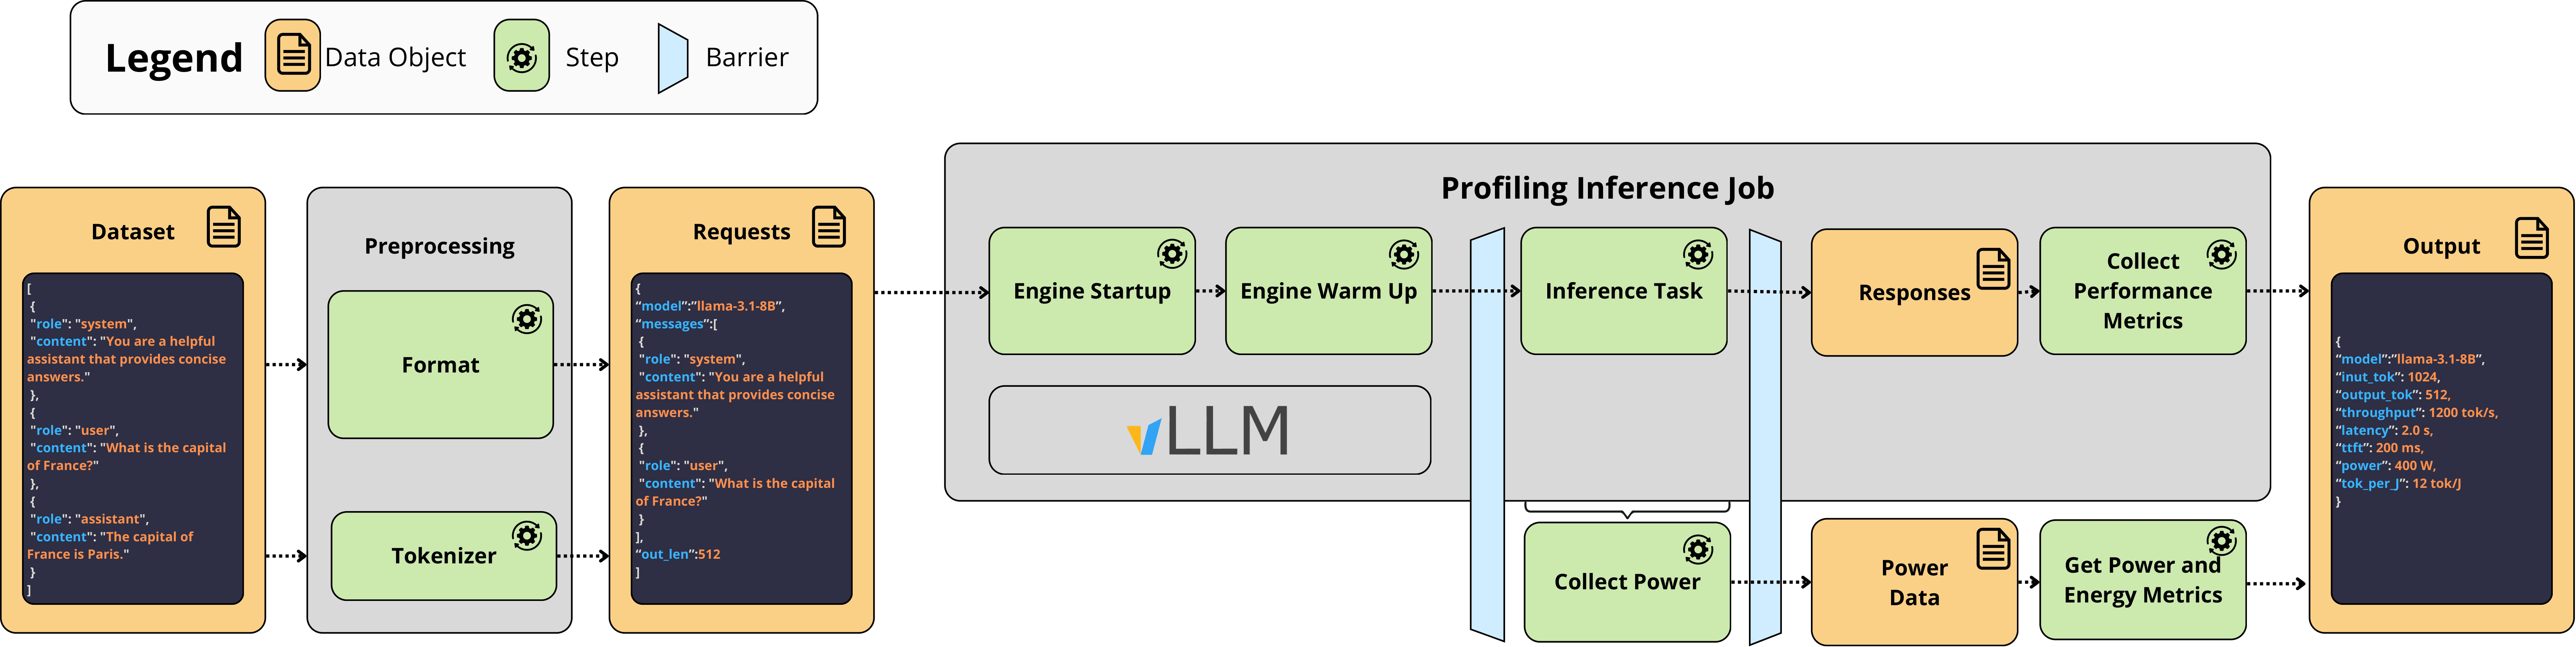
\includegraphics[width=\textwidth]{figs/profile single.png}
    \vspace{5mm}
    \caption{LLM Inference Benchmark Stages.}
    \tagpdfsetup{alttext={LLM Inference Benchmark Stages.}}
    \label{fig:bench}
\end{figure}

To fairly compare those devices, we use a similar software stack on each machine. In particular, we use vLLM \cite{kwon2023efficient}, a high-performance, open-source LLM inference framework compatible with Nvidia, AMD, and Intel GPUs. vLLM allows to achieve superior performance and energy efficiency \cite{fernandez2025energy} compared to the standard Transformers \cite{wolf2019huggingface} implementation by leveraging some key optimizations like the FlashAttention Backend \cite{dao2022flashattention}, PagedAttention \cite{kwon2023efficient}, and continuous batching \cite{agrawal2023sarathi}.
\ref{tab:nodes} reports the specific software stack used on each machine, including the GPU driver, PyTorch version, and vLLM version.

\begin{table}[h!]
\centering
\footnotesize
\caption{GPU nodes used in the experimental evaluation.}
\label{tab:nodes}

\begin{tabularx}{\textwidth}{l l c c c X}
\toprule
\textbf{Vendor} & \textbf{Name} & \textbf{Precision} & \textbf{GPUs/Node} & \textbf{Driver} & \textbf{Software} \\
\midrule

\textbf{NVIDIA} & \textbf{A100}  & BF16, W8A16 & 8  & CUDA 12.6 & \makecell[l]{Torch 2.7.0 \\ vLLM 0.9.0} \\

\textbf{NVIDIA} & \textbf{H100}  & BF16, W8A8  & 4  & CUDA 12.6 & \makecell[l]{Torch 2.7.0 \\ vLLM 0.9.0} \\

\textbf{NVIDIA} & \textbf{GH200} & BF16, W8A8  & 1  & CUDA 12.9 & \makecell[l]{Torch 2.7.0 \\ vLLM 0.9.0} \\

\midrule

\textbf{AMD} & \textbf{MI250}  & BF16        & 4 & ROCm 5.3 & \makecell[l]{Torch 2.7.0+rocm \\ vLLM 0.9.1} \\

\textbf{AMD} & \textbf{MI300X} & BF16, W8A8  & 8 & ROCm 5.3 & \makecell[l]{Torch 2.7.0+rocm \\ vLLM 0.9.1} \\

\midrule

\textbf{Intel} & \textbf{MAX 1550} & FP16 & 6 & oneAPI 2025.2.0 & \makecell[l]{Torch 2.8.0a0 \\ vLLM 0.10.1.xpu} \\

\bottomrule
\end{tabularx}
\end{table}

Each experiment starts by initializing the vLLM engine and loading the inference dataset.
Once the model is loaded and the inference engine is ready, we create an independence process that probes the vendor system monitoring interfaces (py3nvml for NVIDIA, amdsmi for AMD, and xpu-smi for Intel) at consistent intervals to capture power consumption, memory usage, and GPU utilization. For NVIDIA and AMD devices, we sample every 0.5 seconds. For Intel, we have an average sampling rate of 1.9 seconds, due to the longer response time of xpu-smi.
We created the profiler and submitted the inference dataset as a unique batch job to the engine using the vLLM chat method.
Once vLLM has generated the replies for each entry of the dataset, it returns an output object containing information about the end-to-end latency, time to first token, and input and output length of each sequence. This information allows us to collect all the performance metrics described in Section \ref{chap:methods:sec:metrics}.
The profiler data, on the other hand, is used to collect power and energy consumption. To ensure that the profiler process probes the GPU's SMIs only when the GPU is active, we synchronize it with the main process using Python multiprocessing barriers.

For each GPU, this experiment uses different models, precisions, and batch sizes.

Concerning the models, we us four open-source models with a size that ranges from 8B to 32B parameters. Precisely, Llama 3.1 8B, Qwen3 14B, Mistral Small 3.1 24B, and Qwen3 32B. The architectural details of those models are reported in \ref{tab:models}, in the next section.

To evaluate different precisions, we rely on vLLM dynamic weight quantization, which allows us to perform W8A16 quantization (8-bit weights and 16-bit activations) or W8A8 quantization (8-bit weights and 8-bit activations) \cite{vllm-fp8-docs-v0_5_4}, depending on the hardware architecture.
On NVIDIA H100 and AMD MI300x, which offer in-hardware support for FP8 quantization, we use W8A8 quantization. On Nvidia A100, instead, we employ W8A16. Other devices are not included in those experiments, as they do not support either.
For the 16-bit precision, we use bfloat16 (Brain Float 16) precision on Nvidia and AMD, as it is the default precision of the models. For Intel instead, we convert to FP16; single-key optimizations are not yet supported for bfloat16 precision.
Finally, we repeat each experiment for batch sizes of 16 to 128.
\subsection{Multi GPU Experiments}
\label{chap:methods:sec:multi}

We further evaluate LLM inference on GPUs by scaling out to multi-GPU inference.

Multi-GPU parallelism allows for expanding the evaluation in two directions: first, it enables evaluation of significantly larger models compared to single-GPU, thanks to model weight sharding across devices. This also allows a further study of performance scaling with model size. To do so, we include all the models presented in \ref{tab:models}.
Second, as discussed in Section \ref{chap:background:sec:serving}, multi-GPU inference can be implemented using several parallelization strategies, including Tensor Parallelism, Expert Parallelism, and Data Parallelism. As detailed in Section \ref{chap:methods:sec:multi}, these techniques increase the system’s parallel throughput and memory bandwidth approximately linearly with the number of accelerators. Combining these methods introduces a trade-off between the lower communication overhead of Data Parallelism and the greater available memory provided by Tensor Parallelism.

\begin{figure}[h!]
    \centering
    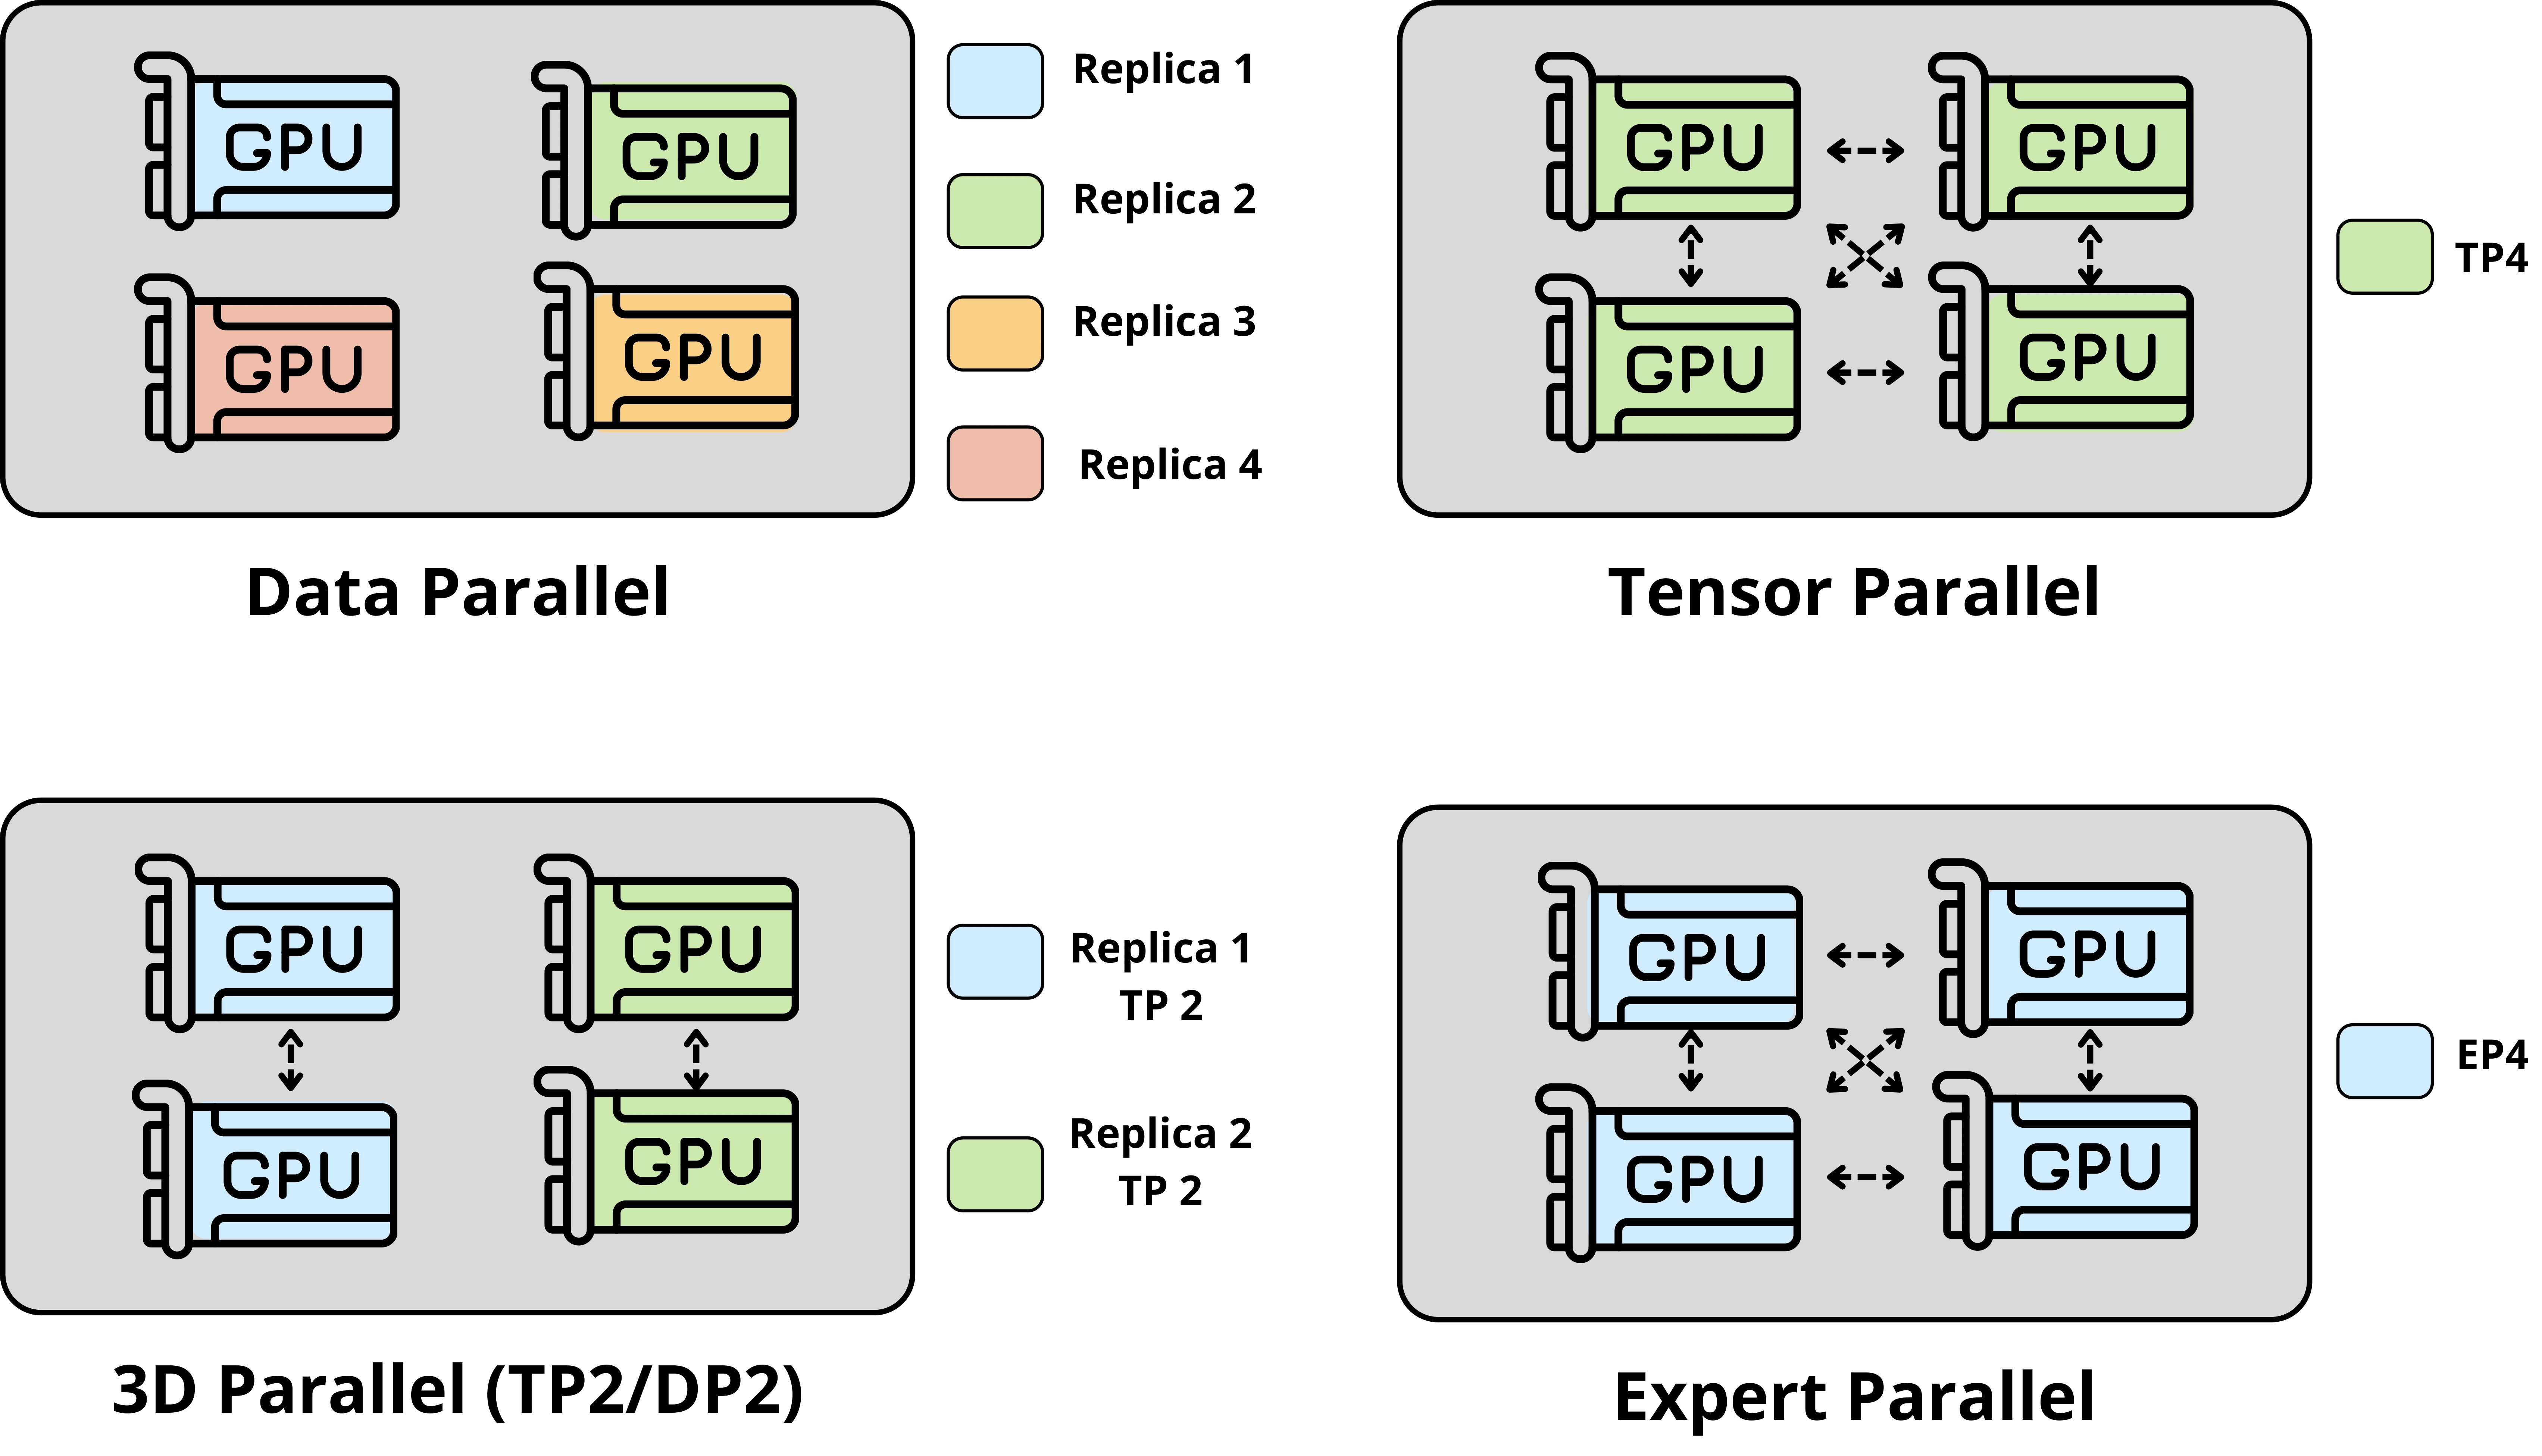
\includegraphics[width=0.85\textwidth]{figs/partition.png}
    \vspace{5mm}
    \caption{Partitioning a node with 3D parallelism.}
    \tagpdfsetup{alttext={Partitioning a node with 3D parallelism.}}
    \label{fig:partition}
\end{figure}

Achieving optimal node-level performance thus requires balancing the number of Data Parallel (DP) replicas and the Tensor Parallel (TP) width per instance, depending on the model size and hardware characteristics. In this study, we explore various TP/DP configurations to empirically determine near-optimal settings. \ref{fig:partition} shows multiple options for partitioning the resources of a 4-GPU node.

\begin{figure}[h!]
    \centering
    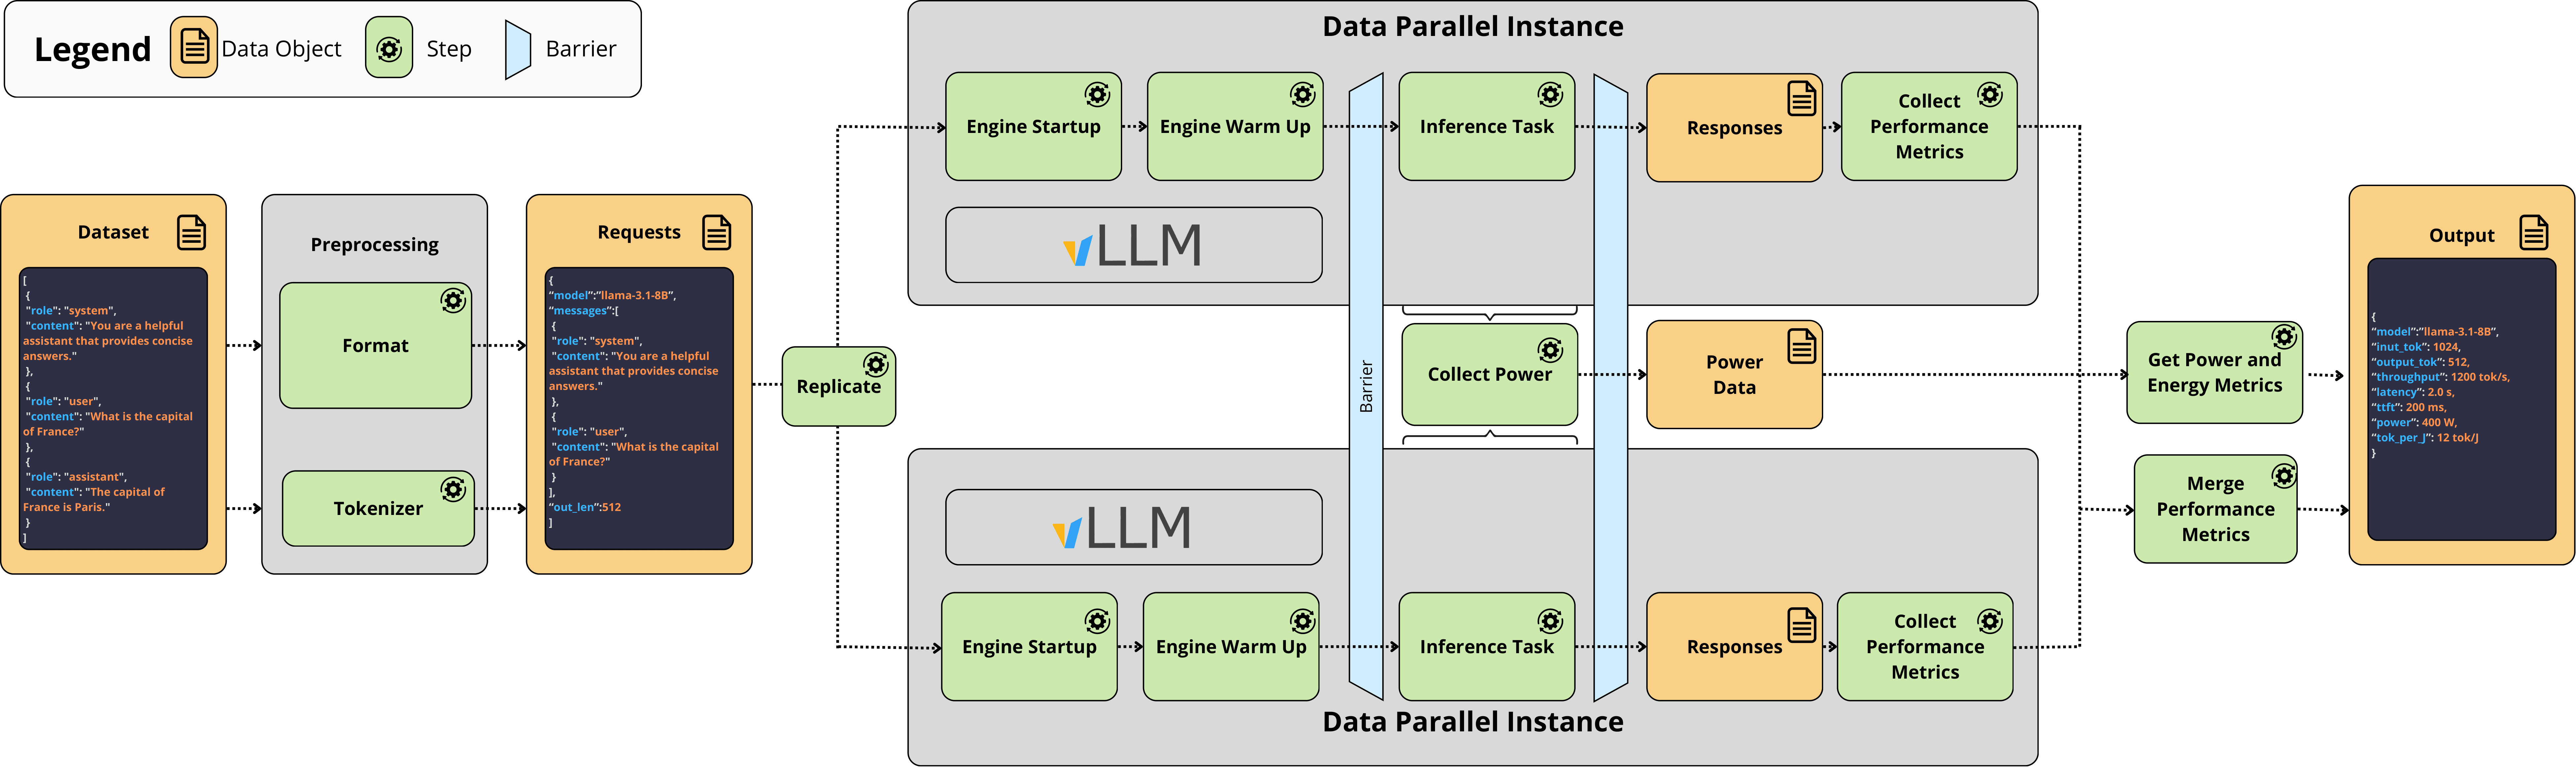
\includegraphics[width=\textwidth]{figs/profile multi.png}
    \vspace{5mm}
    \caption{LLM Inference Benchmark Stages. Multi-GPU setup.}
    \tagpdfsetup{alttext={LLM Inference Benchmark Stages. Multi-GPU setup.}}
    \label{fig:bench}
\end{figure}

An experiment with Data Paralle Size $D$ and Tensor Parallel Size $T$ begins by creating $D$ worker processes and one profiler process. Similar to the single-GPU setup, the profiler process probes the vendor-specific system monitoring interface at consistent intervals to retrieve power consumption data.
Each worker process, instead, initiates a vLLM instance with Tensor Parallel Size $T$. Setting $T\times D = N$, where $N$ is the number of GPUs of the node, allows for an even partition into $D$ homogenous portions, as shown by \ref{fig:partition}.

Once all the $D$ instances are ready, each one starts processing a full instance of the dataset, scaling the single-GPU experiment weakly. When all instances have finished generating replies, their outputs are combined to extract performance metrics, and the profiler process is terminated.

We repeat this experiment with Tensor Parallel Size $T \in \{1, 2, 4\}$ on three multi-GPU nodes: one Sophia bigmem node, featuring 8 DGX A100 80GB GPUs, and two JLSE testbed nodes, featuring 4 NVIDIA H100 SXM5 and 8 AMD Instinct MI300X, respectively. The Data Parallel Size $D$ is set to fully utilize the node. 
The global batch size is set to $128 \times N$, meaning that each of the $D$ instances has a batch size of $128\times T$.
We evaluate both bfloat16 precision and FP8 quantization, using W8A8 on Nvidia H100 and AMD MI300x, and W8A16 on Nvidia A100.

These weak scaling settings allow us to have cleaner performance scaling in two ways. First, it maintains consistency in context lengths across data-parallel instances, since all replicas process identical sequences. Second, it maintains a constant batch size per GPU, ensuring that the number of generated tokens per forward pass remains unchanged across different TP/DP configurations.

\subsection{Comparing Tensor and Expert Parallelism}

We further investigate parallelization strategies for Mixture-of-Experts (MoE) models by comparing Tensor Parallelism (TP) and Expert Parallelism (EP).

Our evaluation includes four large MoE models — Llama4 Scout, Mixtral 8×22B, Qwen 235B A22B, and DeepSeek R1 — all tested in FP8 precision on NVIDIA H100 and AMD MI300x nodes.

Experiments are conducted across varying batch sizes, using a single instance (Data Parallel size = 1) with four GPUs per instance. We first test with a Tensor Parallel size of 4, followed by an Expert Parallel size of 4. The profiling methods used are consistent with those employed in the previous experiment. For DeepSeekR1, we also experimented with 8 GPUs.

\subsection{Dataflow Accelerators Experiments}
\label{chap:methods:sec:dsa}

We investigate LLM inference on hardware accelerators using two dataflow machines: a SambaNova Systems SN40L-16R node \cite{Prabhakar2024}, featuring 16 4th-generation RDUs, and a Cerebras CS3 system \cite{Lie2023} featuring the third-generation Wafer Scale Engine (WSE3). The details of those accelerators are discussed in Section \ref{chap:background:sec:dflow}.

While GPUs are characterized by many streaming multiprocessors that share a common hierarchical memory, dataflow accelerators feature a tiled array of interconnected processing elements, allowing for the mapping of computational graphs into the hardware fabric. This dataflow approach enables reliance solely on fast local scratchpad memories and explicit communication between cores, rather than using a hierarchical cache system as in GPUs, thereby reducing the latency of memory accesses.

Unlike the GPU experiments, which all leveraged vLLM, we utilize a different proprietary inference framework for each dataflow accelerator.

For the Cerebras CS3 system, we use an early-prototype proprietary inference engine that can be queried through an OpenAI-style API.
We task the engine with processing the entire inference dataset by creating one request per conversation.
The Cerebras inference engine supports running models that host weights, activations, and KV caches entirely in on-chip memory to achieve optimal performance. Compared to the streaming-weight approach used for training, this limits the memory capacity to 44GB per CS3 system. For this reason, we limit our analysis to  Llama 3.1 8B.

We repeat the experiment for different batch sizes, ranging from 1 to 8.
To match the engine's effective batch size, we instantiate a corresponding number of clients that send a new request immediately after receiving a response, with the dataset evenly partitioned across clients.
The latencies reported in the responses sent to clients are used to obtain performance metrics.

Regarding power, we collect measurements at the WSE chassis level for all power readings, including the power drawn by the host CPU, WSE, and other supporting components.

For the SambaNova SN40L, we use the SambaStudio inference engine, which can be queried through an OpenAI-compatible interface. Similar to the Cerebras CS3 experiments, we evaluate batch sizes from 1 to 8, creating a number of clients to match the engine's effective batch size.
For this accelerator, we evaluate both Llama 3.1 8B and Llama 3.3 70B.

Regarding power readings, we rely on the PDU-level power consumption for each RDU.
\chapter{Results}
\label{chap:results}

In this chapter, we present the experimental results of our performance and energy-efficiency evaluation of modern datacenter AI accelerators. Following the structure introduced in Chapter~\ref{chap:methods}, we organise the discussion into three parts: Single-GPU experiments (Section~\ref{chap:results:sec:single}), Multi-GPU experiments (Section~\ref{chap:results:sec:multi}), and an analysis of dataflow AI accelerators (Section~\ref{chap:results:sec:dsa}).


\section{Single GPU Experiments}
\label{chap:results:sec:single}

In this section, we discuss the performance of LLM inference on a single GPU, comparing six different GPUs from Nvidia, AMD, and Intel.
We analyze three key performance metrics: End-to-end latency, Time to First Token (TTFT), and Throughput.
For energy efficiency, we utilize Tokens per Joule as the metric.

\ref{fig:all_metrics_1gpu} shows how performance and energy efficiency evolve with batch size across 6 different GPUs and four LLM models running with half (16-bit) precision. Multi-Tile GPUs (AMD MI250 and Intel Max 1550) use tensor parallelism to fully utilize their resources.
From those experiments, we can extract three main insights: 
(1) a cross-vendor comparison of the performance and energy efficiency of GPU models, \
(2) the trend of performance and energy efficiency as model size grows, and 
(3) the trade-off between latency and throughput across different batch sizes.

\begin{figure}[h]
    \centering
    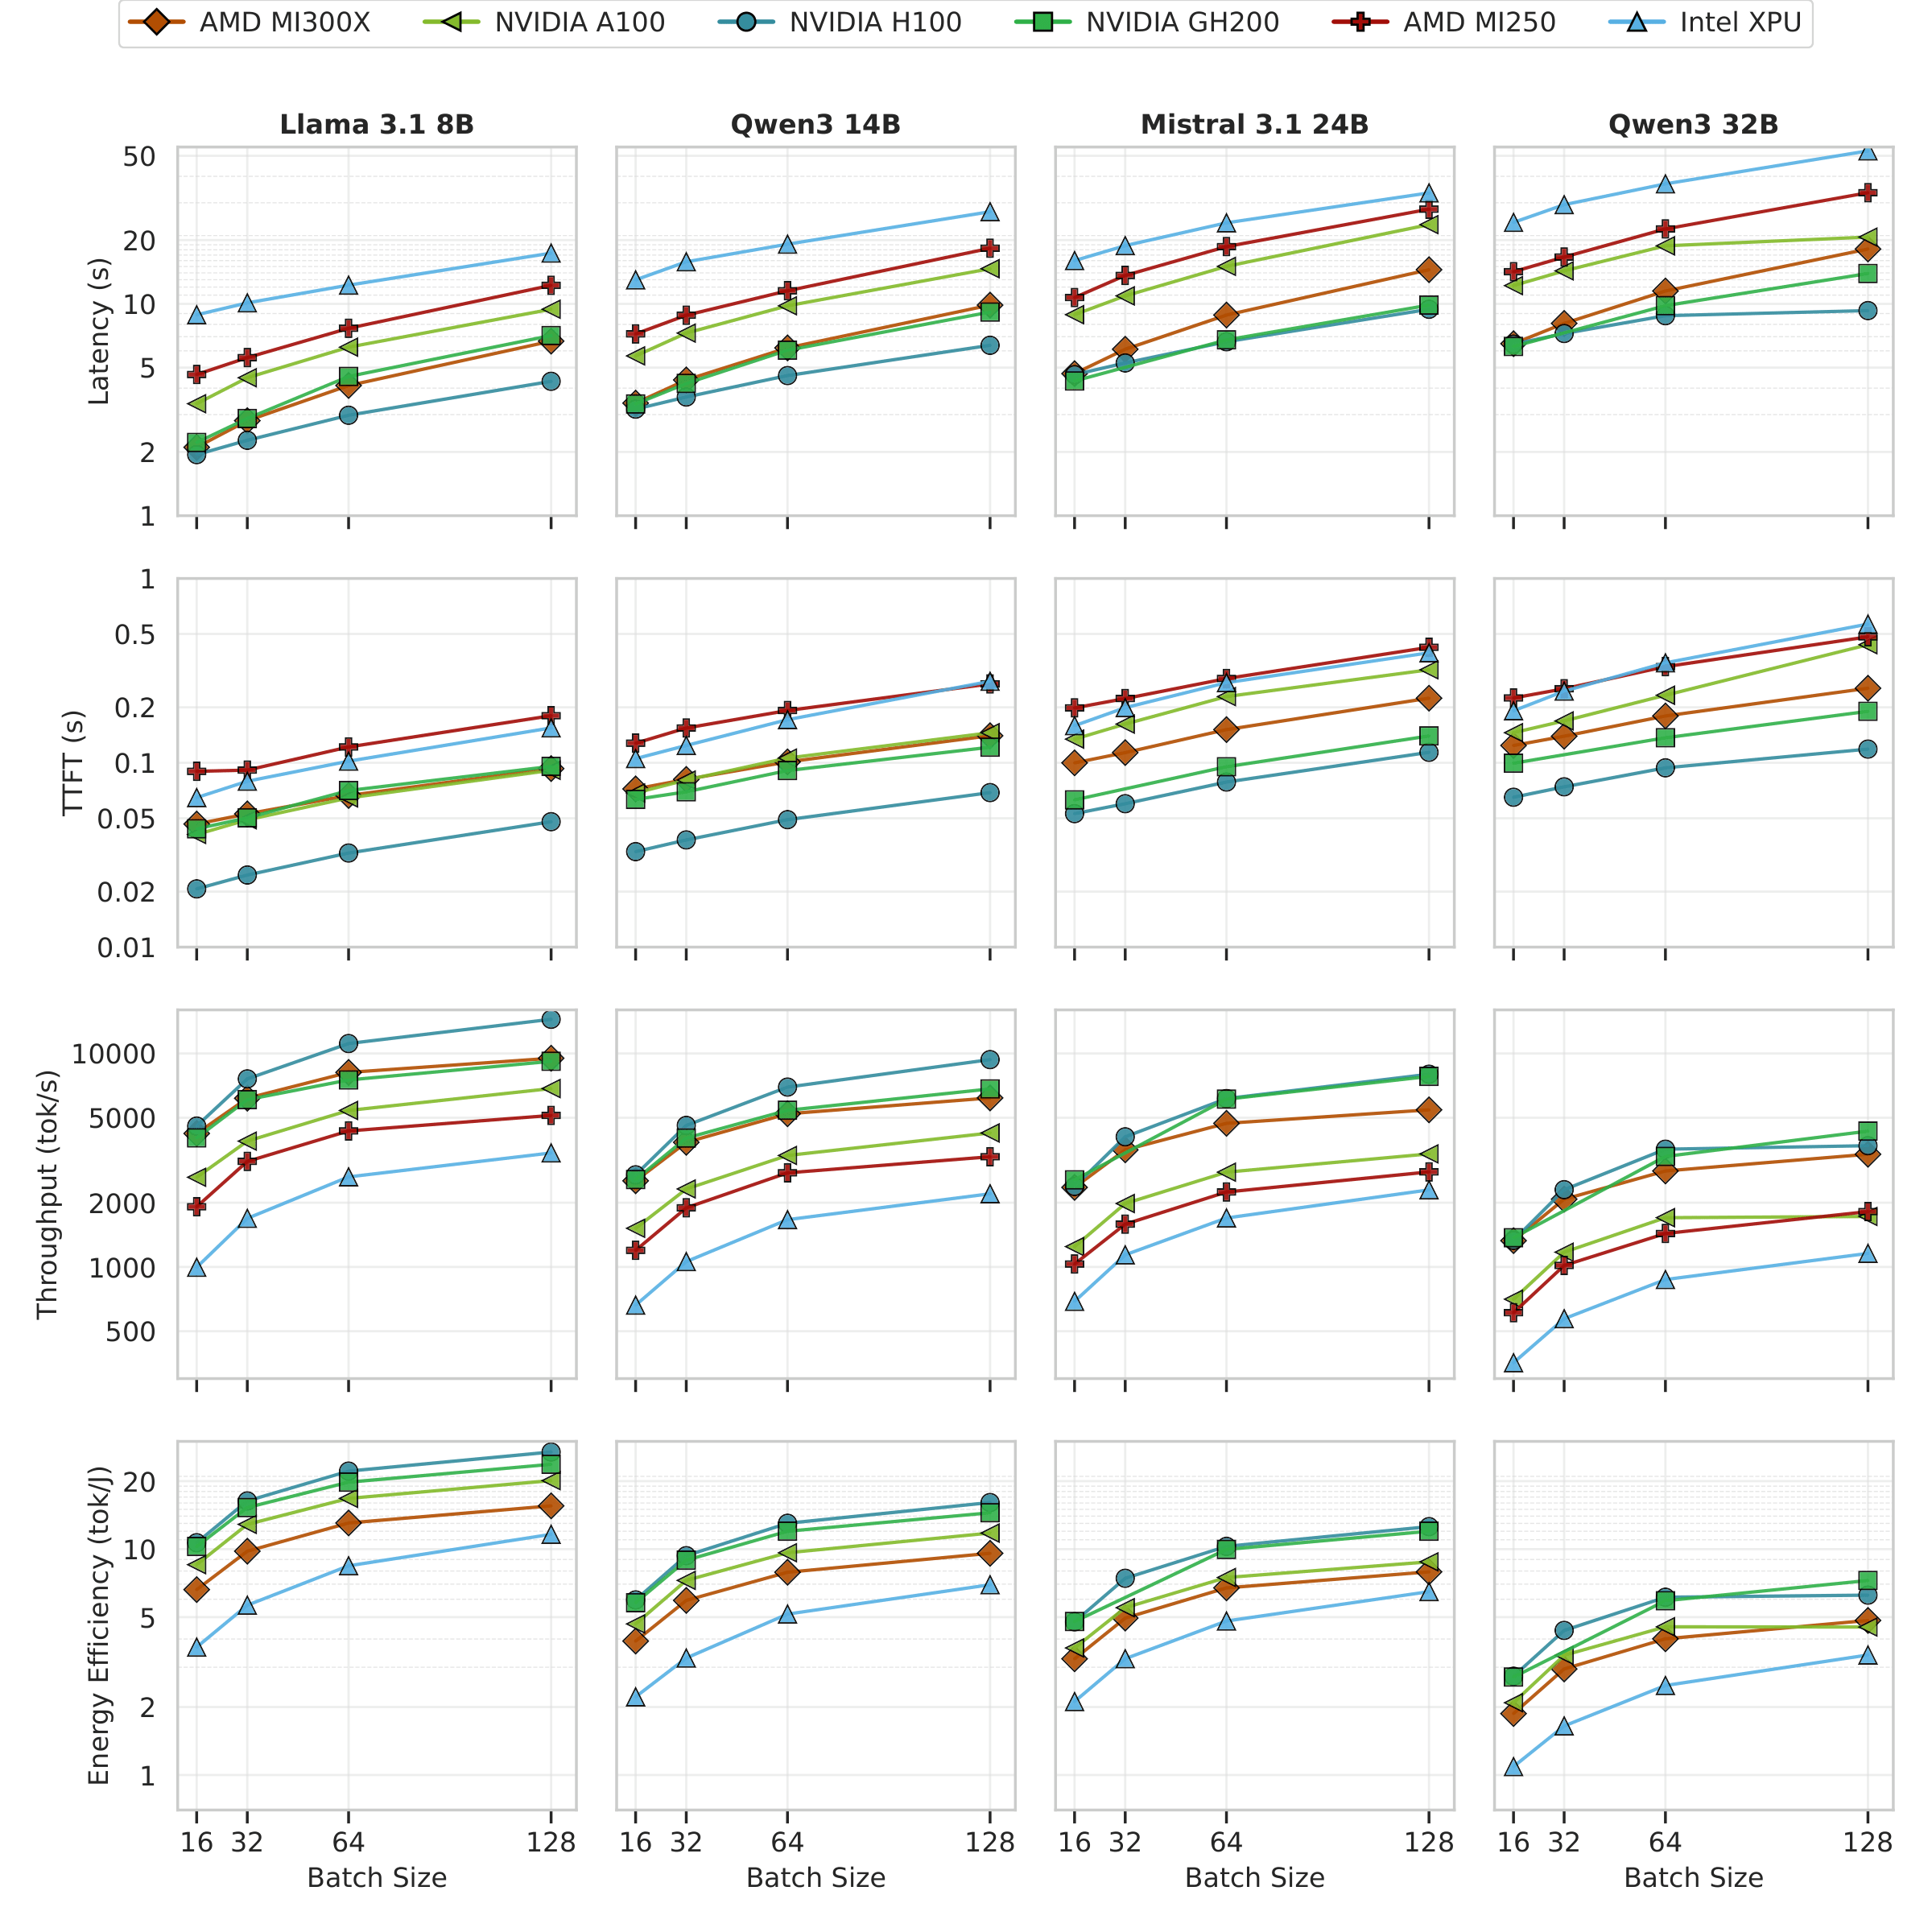
\includegraphics[width=\textwidth]{figs/combined_performance_plots.png}
    \caption{The evolution of performance and energy efficiency with batch size across six GPUs.}
    \tagpdfsetup{alttext={The evolution of performance and energy efficiency with batch size across six GPUs.}}
    \label{fig:all_metrics_1gpu}
\end{figure}

\subsection{GPU model comparison}
For this analysis, we use the NVIDIA A100 as the natural performance baseline, as it is both the oldest and most widely used GPU among those tested. Both Nvidia Hopper (H100 and GH200) and AMD CDNA3 (MI300x) GPUs consistently outperform the A100 baseline in terms of performance, across models and batch sizes. The AMD MI250 and the Intel Max 1550, instead, are both outperformed by the Ampere GPU. Importantly, both GPUs feature larger memories than their Nvidia counterparts (128 GB compared to 80 GB), which leads to two main benefits. First, they support running larger models, and second, they substantially narrow the throughput gap as model size and batch size increase. In fact, especially with the larger 32B model, Nvidia A100 and H100 saturate their throughput at batch size 64 due to the insufficient memory available for KV cache.
Concerning the increased latency and the lower throughput, it is also important to mention that each Intel Max 1550 and AMD MI250 is constituted of two GPU tiles and thus requires frequent all-gather operations between the two to fully utilize its compute power. This is particularly detrimental in small models, advantaging monolithic GPUs.

Regarding energy efficiency, Nvidia Hopper GPUs demonstrate an improvement over the previous generation, despite their increased average power consumption. In fact, where the Nvidia A100 had a TDP of 400W and an average power consumption of 337W, the Nvidia H100 has a TDP of 700W and consumes, on average, 478W. Nevertheless, the substantial decrease in latency is sufficient to compensate for the increased power consumption.
The same does not hold for AMD MI300x, which consistently surpasses the A100 in raw performance but achieves lower energy efficiency. Notably, the AMD MI300x has the highest power consumption among the GPUs tested (750W TDP and 625W average power consumption).
The Intel Max 1550 exhibits higher latency and increased power consumption compared to the Nvidia A100, resulting in lower energy efficiency.

AMD MI250 and Intel Max 1550 underperform relative to the NVIDIA A100 despite their higher power consumption. This gap is partly due to their multi-tile designs, which require tensor parallelism to fully utilize the hardware, as each tile is presented to the operating system as a separate device. Additionally, the AMD and Intel implementations of vLLM currently lag in software maturity, lacking support for key optimizations. In terms of energy efficiency, the Intel Max 1550 is less efficient than the A100, while no data is available for the AMD MI250.

Memory capacity is another critical factor. NVIDIA GPUs rank lowest in VRAM, which limits the size of models they can host compared to the other GPUs under analysis. The AMD MI300x provides the largest memory capacity at 192GB, enabling a single device to run 70B-parameter models. It is also important to note that the current vLLM implementation does not utilize all the unified memory of the GH200 SoC, which limits the memory capacity to 96 GB of VRAM, resulting in comparable performance to the base NVIDIA H100.

NVIDIA Hopper GPUs emerge as the most performant and energy-efficient GPU among those tested. The AMD MI300X also displays competitive performance, outpacing the NVIDIA A100 in terms of performance, but not in energy efficiency. Intel Max 1550 and AMD MI250 offer lower performance and energy efficiency than NVIDIA A100.

\begin{figure}[H]
    \centering
    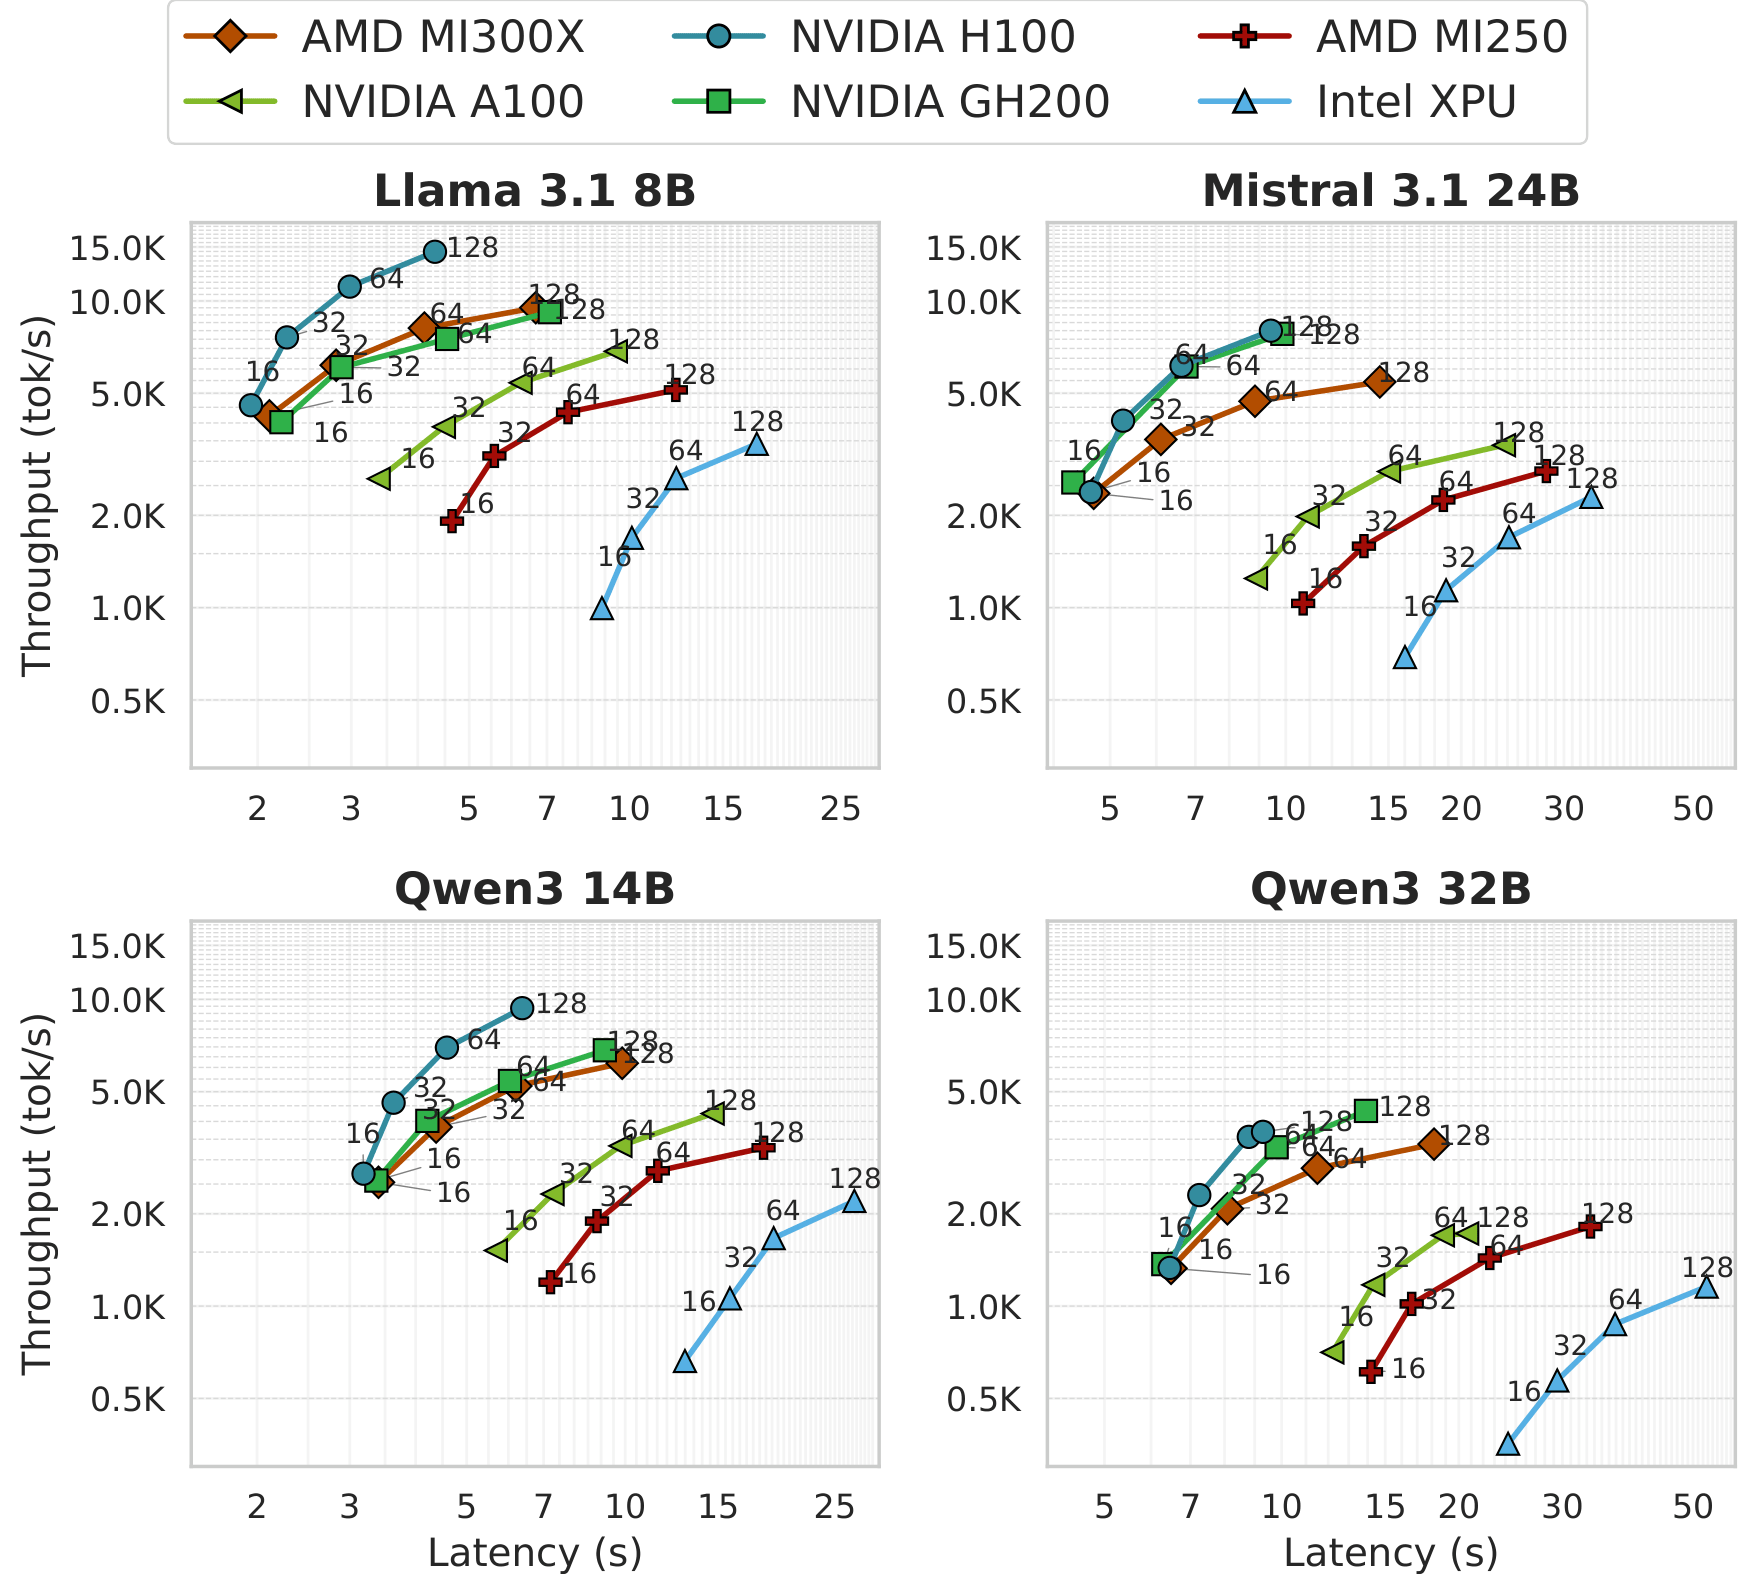
\includegraphics[width=0.9\textwidth]{figs/throughput_latency_plot.png}
        \caption{Trade-off between throughput and latency across batch sizes (16-128), using four LLM models and six different GPUs. The numbers in the plots indicate the batch sizes.}
        \tagpdfsetup{alttext={Trade-off between throughput and latency across batch sizes (16-128), using four LLM models and six different GPUs. The numbers in the plots indicate the batch sizes.}}
    \label{fig:bs}
\end{figure}

\subsection{Batch Size} 
\ref{fig:bs} presents a different perspective on our evaluation data, enabling us to better understand the impact of batch size. The x-axis represents the average end-to-end latency of sequences, while the y-axis represents throughput. These representations allow us to observe the trade-off that happens under varying batch sizes.
Consistent with the analysis in Chapter \ref{chap:methods:sec:model}, we observe that across all GPU models, smaller batches result in lower latency due to reduced computation at each forward pass.
In fact, the number of FLOPs to be executed at each forward pass scales linearly with batch size $b$. However, the model weights have to be loaded from off-chip memory independently of $b$. This causes the compute-related part of latency to decrease linearly with batch size, while the operational intensity $OI$ (expressed in FLOPs/byte) drops linearly with $b$, making computation more memory-bound and thus harming throughput.

Increasing throughput also strongly correlates with improving energy efficiency.
After adjusting the GPU model and precision, we observe a correlation of 0.92 to 0.99 between energy efficiency and throughput. This is because batch size has a reduced impact on power consumption, whereas it has a significant effect on latency.

From these observations, we conclude that larger batch sizes improve the performance in an offline setting while also achieving better energy efficiency.
In contrast, metrics related to online serving, such as TTFT, ITL, or E2E latency, improve as the batch size decreases, creating a trade-off with energy efficiency. 

\begin{figure}[H]
    \centering
    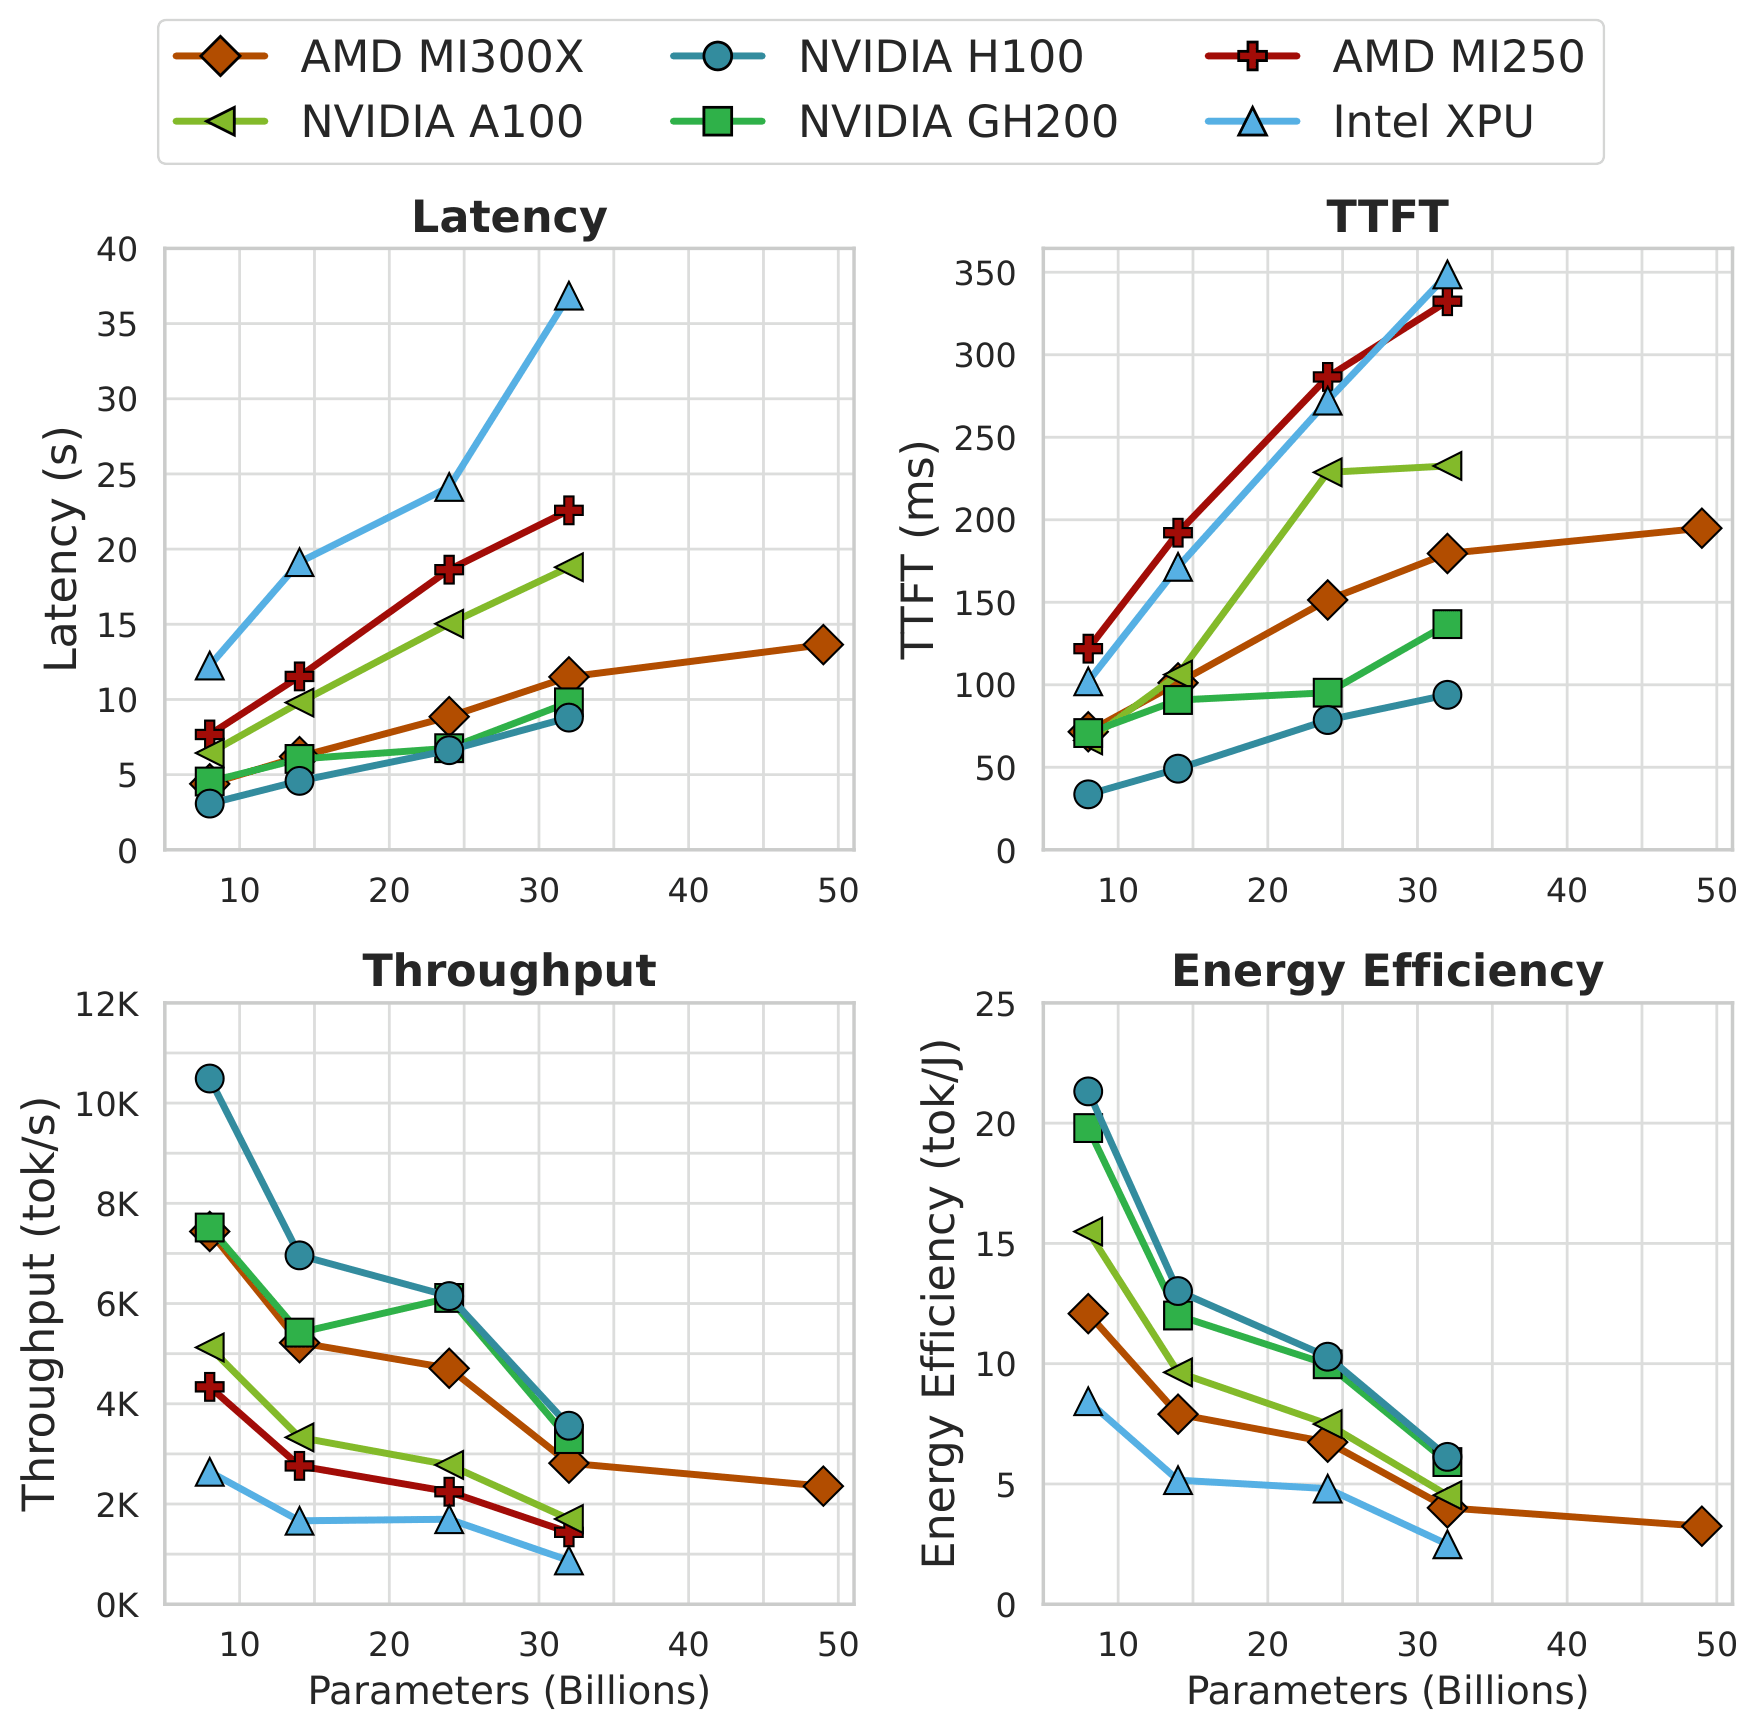
\includegraphics[width=0.7\textwidth]{figs/trend_Latency_TTFT_Throughput_Energy.png}
    \caption{Performance and energy efficiency across six GPUs for models of varying size.}
    \tagpdfsetup{alttext={Performance and energy efficiency across six GPUs for models of varying size.}}
    \label{fig:1gpu_modelsize}
\end{figure}

\subsection{Model Size} 
\ref{fig:1gpu_modelsize} displays a subset of the datapoints from \ref{fig:all_metrics_1gpu}, allowing us to better visualize how the four key metrics analyzed change as the model size increases, with the input dataset and batch size set to 64. 

As a first observation, we can see that latency and TTFT increase linearly with model size, while throughput and energy efficiency decrease inversely.
This trend is consistent with the analysis made in Chapter \ref{chap:methods:sec:model}, which predicts the latency of the forward pass to scale roughly linearly with the model size $N$.

\begin{comment}
\begin{figure}[H]
    \centering
    \includegraphics[width=0.9\textwidth]{figs/fp8_vs_bf16_improvements_subplots.png}
        \caption{  Throughput and energy-efficiency gains (FP8 vs. bfloat16) across four LLM models and four GPUs. The greatest improvement is annotated.}
    \label{fig:fp8}
\end{figure}
\end{comment}

\begin{figure}[H]
    \centering
    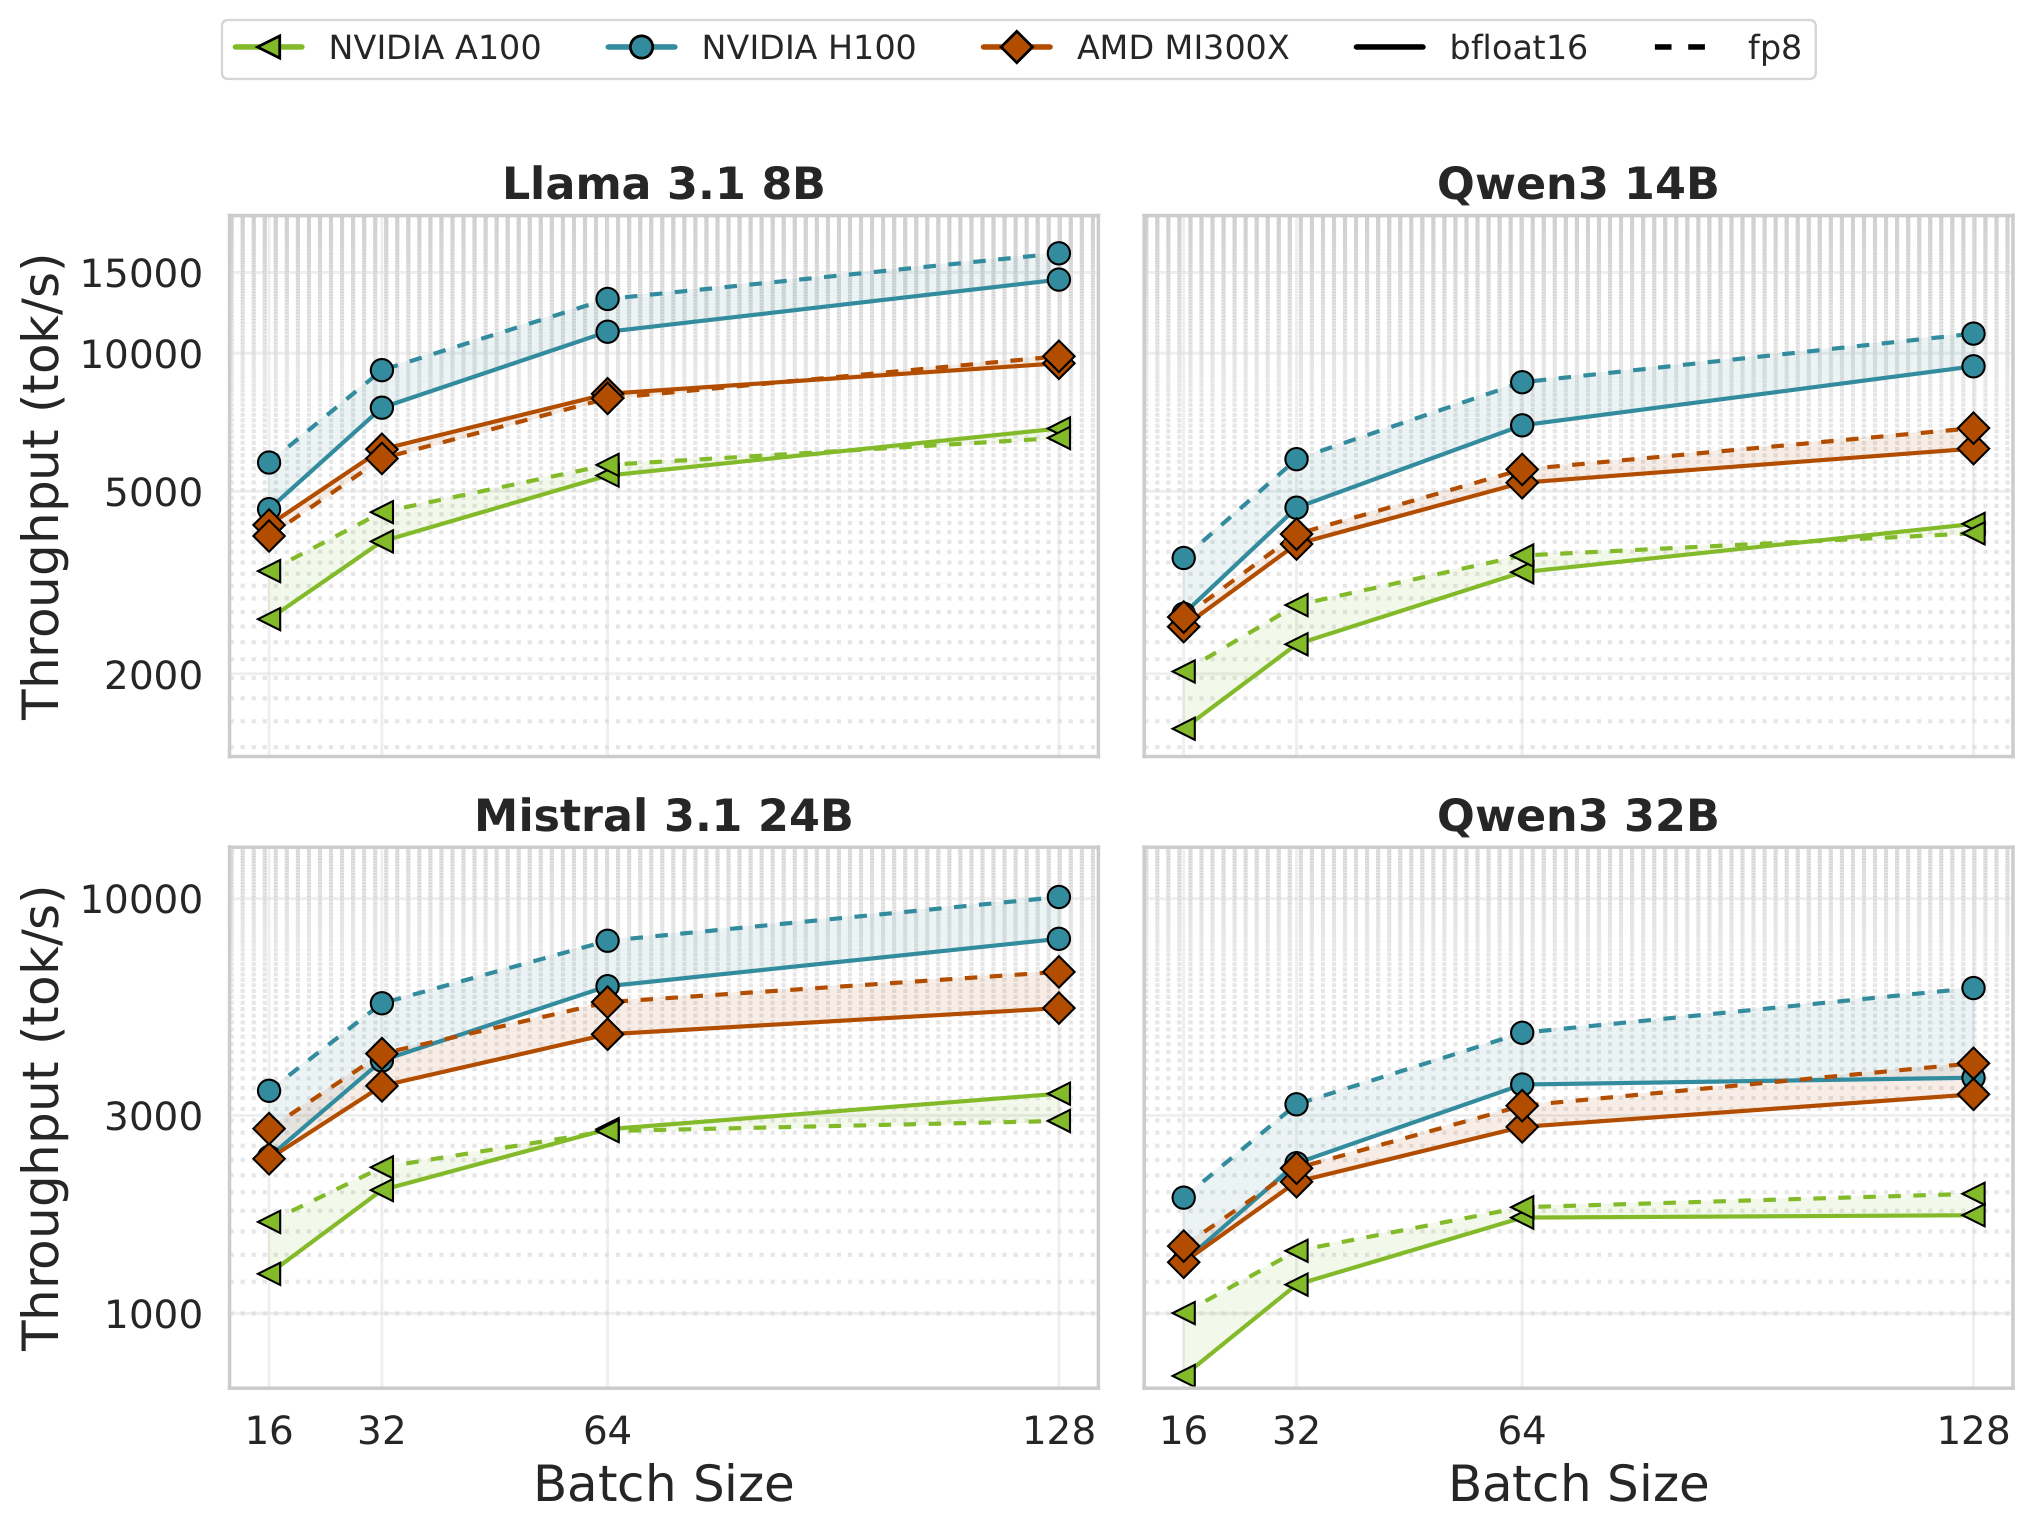
\includegraphics[width=\textwidth]{figs/throughput_by_model_with_precisions_filled.png}
    \caption{Throughput (tok/s) comaprison between bfloat16 and FP8 precision across GPUs and LLM models.}
    \tagpdfsetup{alttext={Throughput (tok/s) comaprison between bfloat16 and FP8 precision across GPUs and LLM models.}}
    \label{fig:fp8bs}
\end{figure}

\subsection{FP8 Quantization}

We evaluate the impact of FP8 quantization on throughput and energy efficiency across four GPU architectures: NVIDIA A100, H100, GH200, and AMD MI300X. \ref{fig:fp8bs} summarizes the results.

NVIDIA A100 does not provide native FP8 support and therefore relies on W8A16 quantization, which applies 8-bit weights and 16-bit activations. Although it cannot exploit FP8-specific functional units, A100 still benefits from the reduced memory footprint of 8-bit weights. In contrast, NVIDIA Hopper (H100, GH200) and AMD MI300X implement FP8 arithmetic natively and can operate with W8A8 precision throughout, yielding more substantial performance gains.

In theory, reducing precision from bfloat16 to W8A8 halves both the arithmetic cost and data movement, suggesting a near 2 $\times$ speedup. In practice, our measurements show that real-world improvements fall well short of this idealized limit. While W8A8 consistently outperforms bfloat16, the magnitude of gains varies significantly across hardware.

NVIDIA Hopper GPUs benefit the most, with throughput improvements of 20\%–38\% and energy-efficiency gains of 34\%–46\%. AMD MI300X shows smaller and more model-dependent improvements: throughput ranges from no gain on Llama 8B to roughly 20\% on Mistral Small 24B; energy efficiency improves by 16\%–35\%. These results highlight the gap between theoretical and practical benefits, underscoring the need for hardware–software co-design to fully exploit low-precision arithmetic.

Batch size also plays an important role. W8A8 quantization becomes increasingly advantageous at larger batch sizes, where arithmetic dominates execution time. Conversely, W8A16 (used on A100) yields its largest gains at small batch sizes, where the workload is more memory-bound, and exhibits diminishing returns as the batch size increases. \ref{fig:fp8bs} illustrates these trends for Qwen3 32B.

Quantization inevitably introduces some loss in model accuracy. While a complete analysis is left for future work, prior results \cite{kurtic2024give} indicate that FP8-quantized models retain more than 99\% of the accuracy of their bfloat16 counterparts on standard benchmarks, suggesting that accuracy degradation is typically minor.

In summary, W8A8 quantization delivers meaningful speedups and energy savings at minimal accuracy cost, with NVIDIA Hopper GPUs achieving the largest benefits (up to 44\% throughput and 47\% energy efficiency). AMD MI300X gains are smaller but often significant for larger models, whereas W8A16 on A100 is most effective at small batch sizes.
\section{Multi GPU Experiments}
\label{chap:results:sec:multi}

In the second part of our evaluation, we examine the performance of multi-GPU inference. We evaluate three multi-GPU nodes featuring 8 NVIDIA A100, 4 NVIDIA H100, and 8 AMD MI300x, respectively.
Each node is tested with three configurations, corresponding to tensor parallel sizes of 1, 2, and 4, and a data parallel size set to fully utilize the node's resources.
Using bfloat16 precision, we evaluate 10 models, while with FP8 quantization, we evaluate 14 LLMs.

The data is presented through two heatmaps (\ref{fig:heatmapbf16} and \ref{fig:heatmapfp8}), structured to have one row per model and three columns per node, corresponding to the different partitions.
The models are sorted by parameter count, while the columns correspond to different models and their TP/DP settings. Throughput is normalized by the number of data parallel instances, while energy efficiency does not need to be normalized due to weak scaling (see \ref{chap:methods:sec:multi}).

This data allows us to observe different trends of multi-GPU inference, including
(1) the scaling efficiency of Data and Tensor Parallelism,
(2) the impact of model size scaling on performance,
(3) a cross-vendor comparison of the three nodes, in a multi-GPU setting.

\begin{figure}[H]
    \centering
    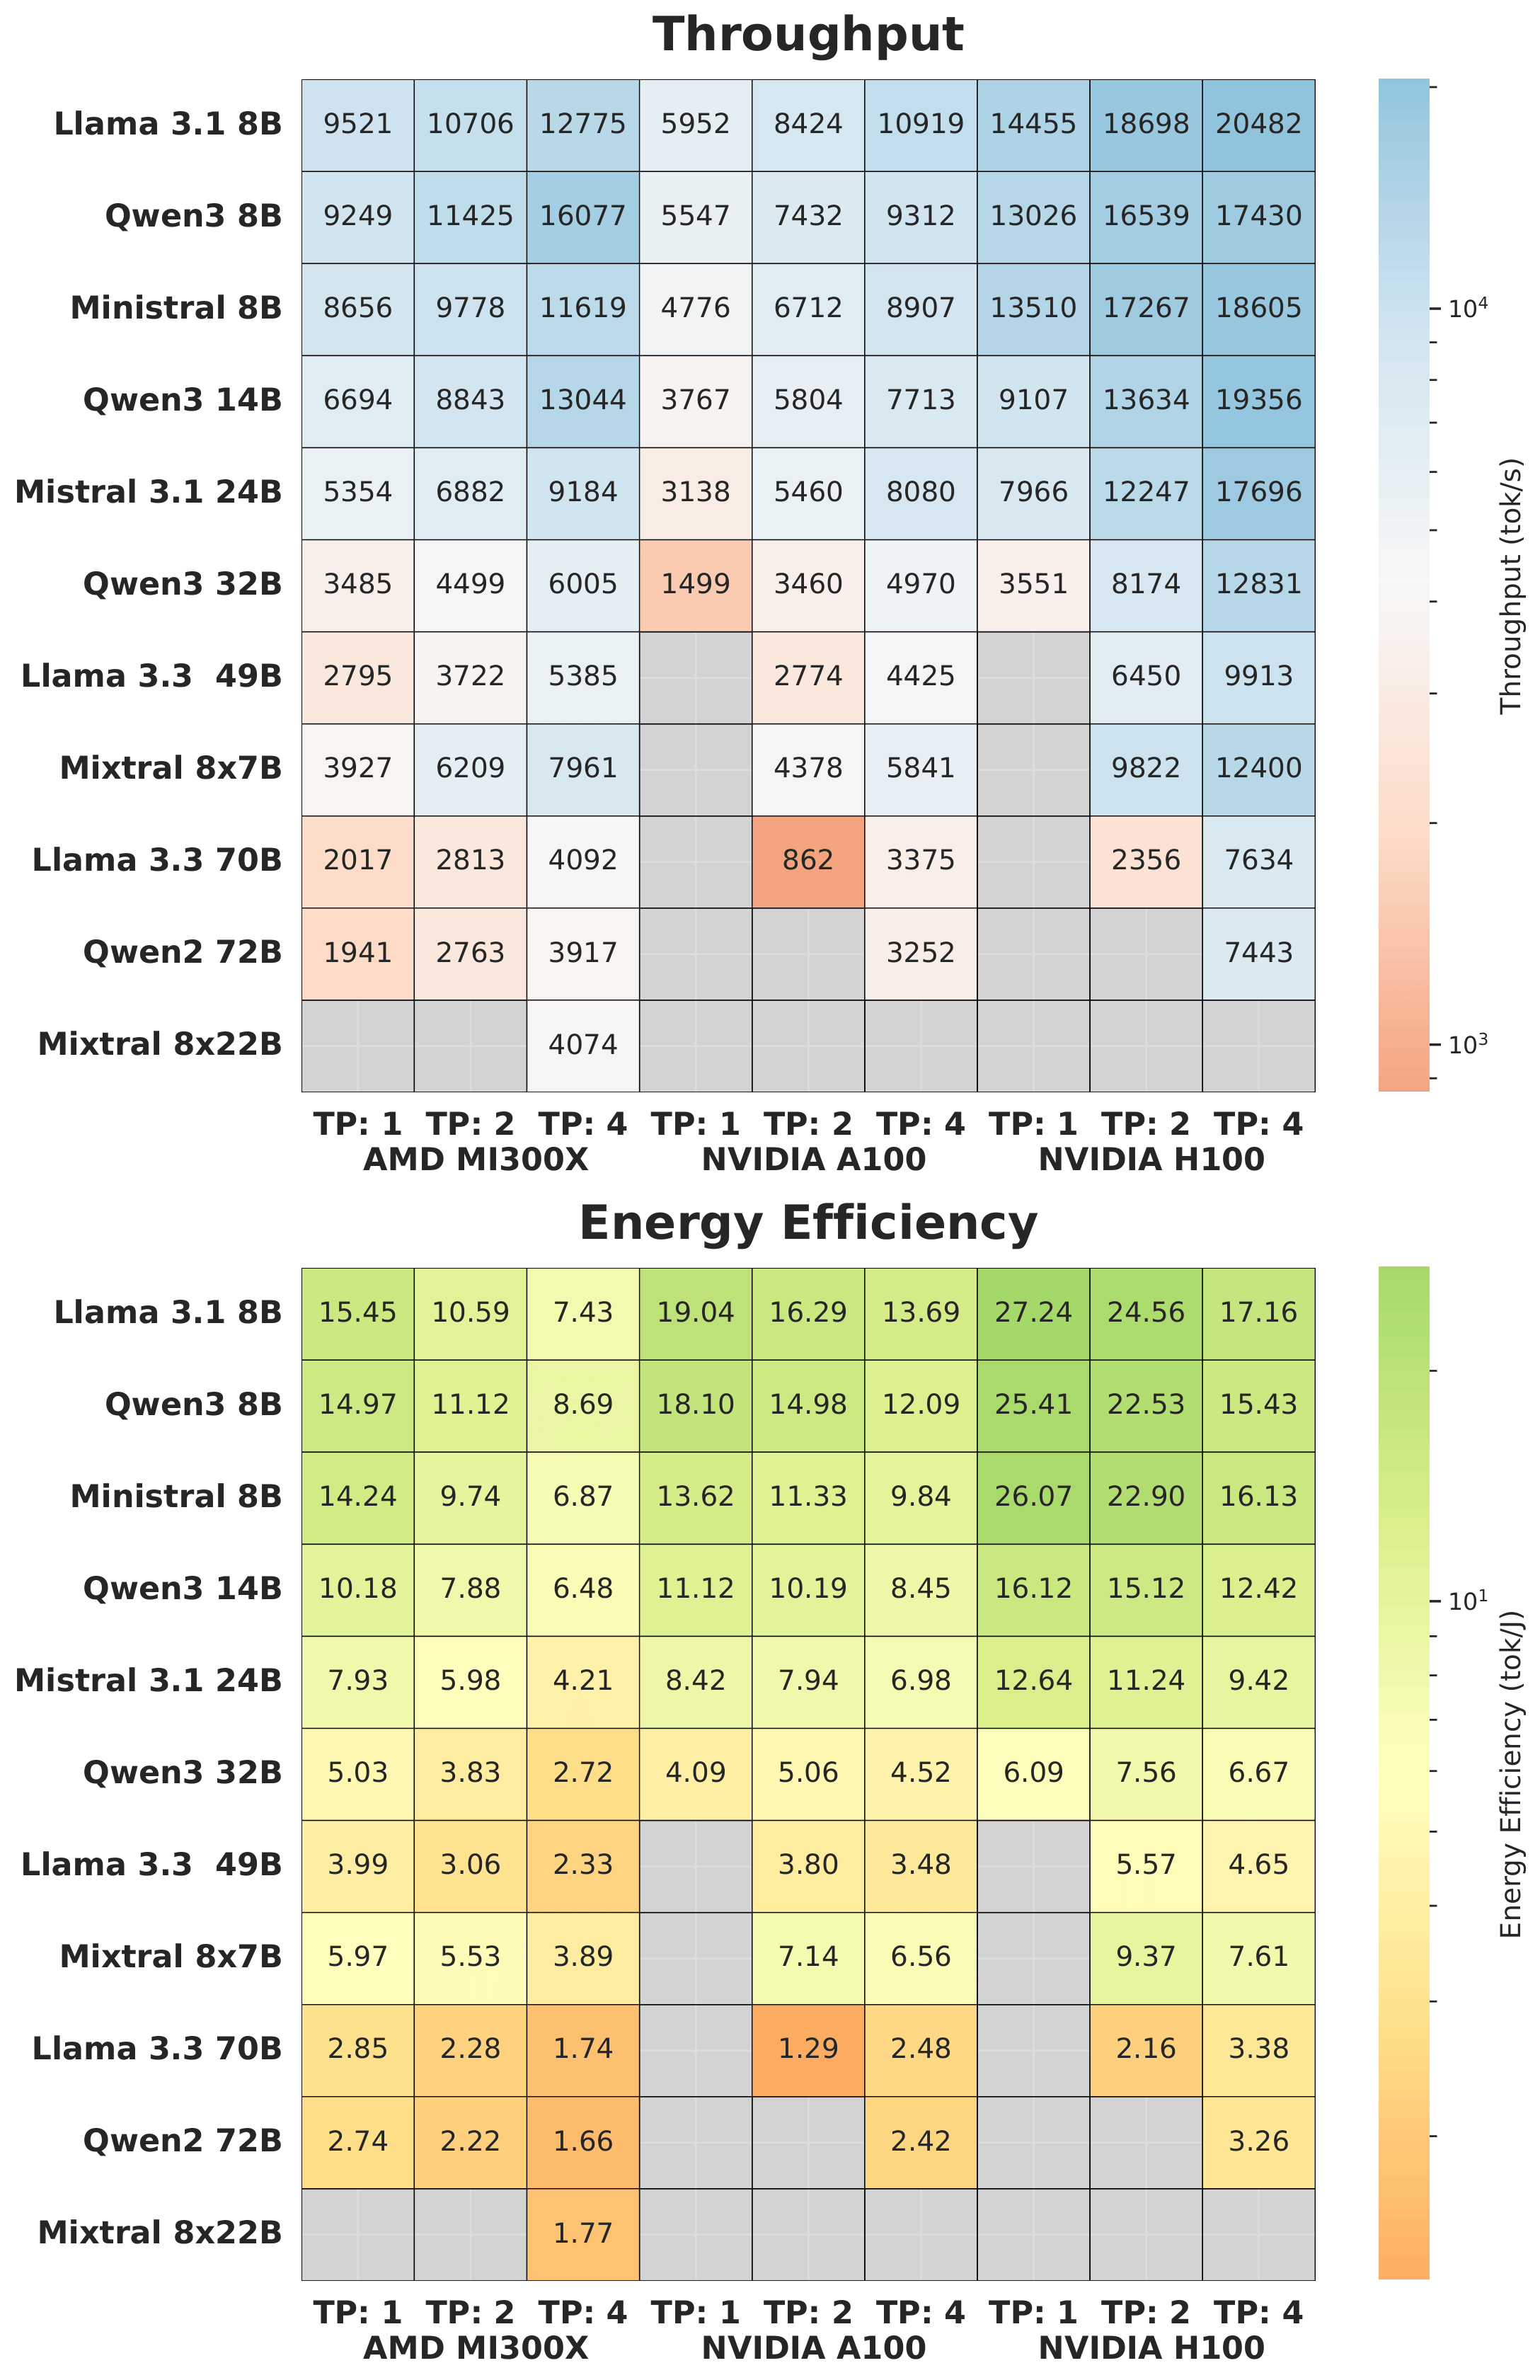
\includegraphics[width=0.9\columnwidth]{figs/heatmap Throughput (toks)_vs_Energy Efficiency (tokJ)_bfloat16.png}
    \caption{Throughput and energy efficiency heatmap across three multi-GPU nodes (bfloat16).}
    \tagpdfsetup{alttext={Throughput and energy efficiency heatmap across three multi-GPU nodes (bfloat16).}}
    \label{fig:heatmapbf16}
\end{figure}

\begin{figure}[H]
    \centering
    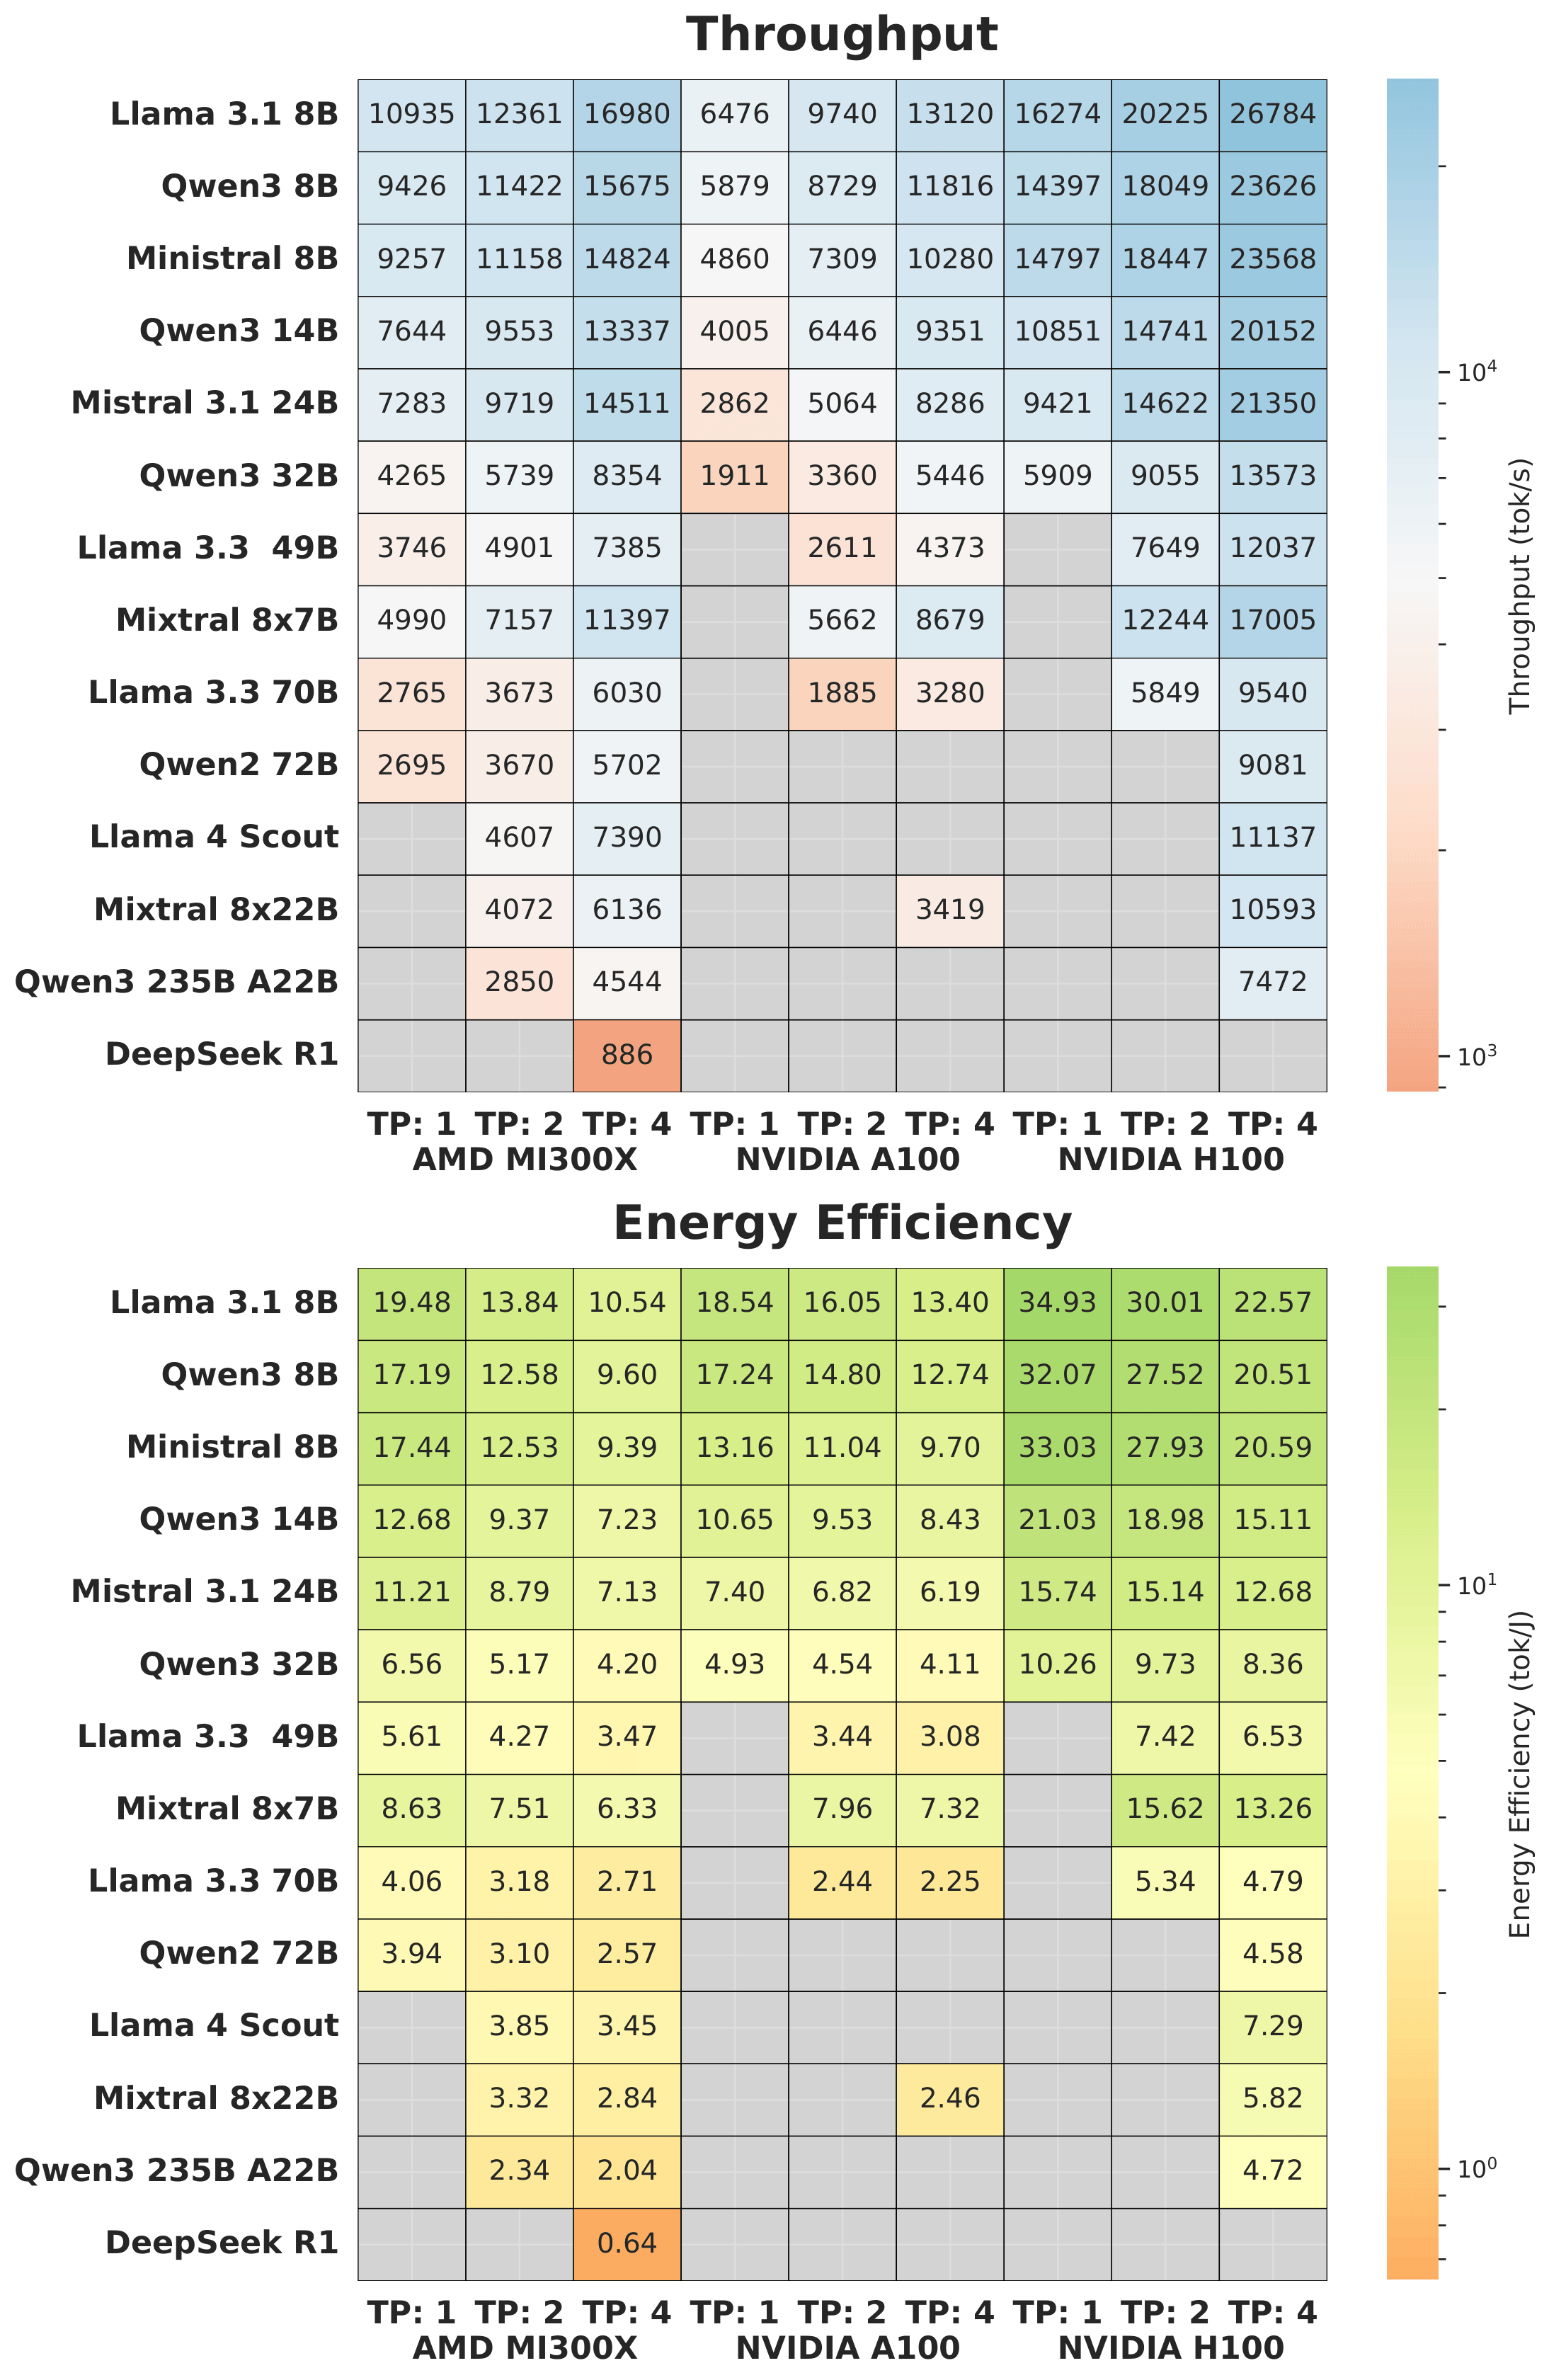
\includegraphics[width=0.9\columnwidth]{figs/heatmap Throughput (toks)_vs_Energy Efficiency (tokJ)_fp8.png}
      \caption{Throughput and energy efficiency heatmap across three multi-GPU nodes (FP8).}
      \tagpdfsetup{alttext={Throughput and energy efficiency heatmap across three multi-GPU nodes (FP8).}}
    \label{fig:heatmapfp8}
\end{figure}


\subsection{Scaling efficiency with 3D Parallelism}
Resource allocation in multi-GPU LLM inference requires balancing memory capacity and computational efficiency when choosing between Tensor and Data Parallelism. As discussed in Section \ref{chap:model:sec:multi}, Tensor Parallelism partitions model weights across GPUs, enabling larger models to run and potentially improving throughput. However, it introduces frequent all-gather operations, which result in synchronization overheads and idle GPU time.

\begin{comment}
\begin{figure}[H]
    \centering
    \includegraphics[width=0.9\columnwidth]{figs/efficiency_lineplot_Throughput per Instance_bfloat16.png}
      \caption{Throughput gain with Tensor Parallelism.}
    \label{fig:tpbars}
\end{figure}
\ref{fig:tpbars} shows how performance improves by increasing the Tensor Parallel size from 1 to 4 in three multi-GPU nodes.
\end{comment}

In our experimental results, we observe that configurations scaled purely with Data Parallelism exhibit an ideal linear scaling.
Instead, configurations that utilize a Tensor Parallel size of 2 or 4 enhance the throughput of the vLLM inference engine; however, display scaling efficiency falls short of the ideal level. Specifically, configurations with Tensor Parallel size 2 yield an average throughput improvement of approximately 33\% (29.9\% on AMD MI300X, 31.4\% on NVIDIA A100, and 37.4\% on NVIDIA H100), while those with Tensor Parallel size 4 achieve about 74\% (73.3\% on AMD MI300X, 74.5\% on NVIDIA A100, and 74.2\% on NVIDIA H100). In terms of scaling efficiency—computed as $\text{Perf}{\text{N-GPUs}} / (N \times \text{Perf}{\text{1-GPU}})$—Tensor Parallel size 2 reaches 65\% efficiency, whereas size 4 reaches 43\%. Compared to data-parallel configurations, which maintain nearly 100\% scaling efficiency, these results indicate that in offline inference scenarios, increasing the number of data-parallel instances is generally more effective for maximizing both throughput and energy efficiency than increasing tensor parallelism.

There are, however, notable exceptions to this general trend. When the model size is large enough that the weights occupy most of the available VRAM, the remaining memory becomes insufficient to support large batch sizes. In such cases, vLLM manages the limitation in two ways: it either dynamically reduces the effective batch size relative to the configured engine setting or, in the event of out-of-memory errors, performs expensive recomputations of segments of the KV matrices. As a result, models that utilize more than 80\% of GPU memory tend to achieve better performance with higher Tensor Parallelism configurations, sometimes even exceeding 100\% scaling efficiency. For instance, Qwen3 32B exhibits higher scaling efficiency with a tensor parallel size of 2 on both NVIDIA A100 and H100 nodes. Similarly, the substantial memory requirements of Llama 3.3 70B make a tensor parallel size of 4 preferable to 2 on the same hardware.

Regarding energy efficiency, a consistent pattern is evident. Data-parallel configurations demonstrate energy efficiency comparable to single-GPU setups, while configurations employing tensor parallelism tend to be less efficient. An exception again occurs for models that use more than 80\% of the available VRAM. As discussed earlier, when hardware remains constant, energy efficiency shows a strong positive correlation with throughput, with correlation coefficients ranging from 0.90 to 0.94. Therefore, optimizing throughput inherently leads to improvements in energy efficiency.

It is also noteworthy that Tensor Parallel configurations generally draw less power on average, as illustrated in \ref{fig:powbars}. However, this reduction in power consumption is insufficient to offset the performance degradation caused by inter-GPU communication overhead. In the specific cases where higher tensor parallelism yields better performance, the lower power usage contributes to energy efficiency gains that exceed the corresponding throughput improvements. This observation further highlights the importance of maintaining sufficient memory capacity for the KV cache.

\begin{figure}[h!]
    \centering
    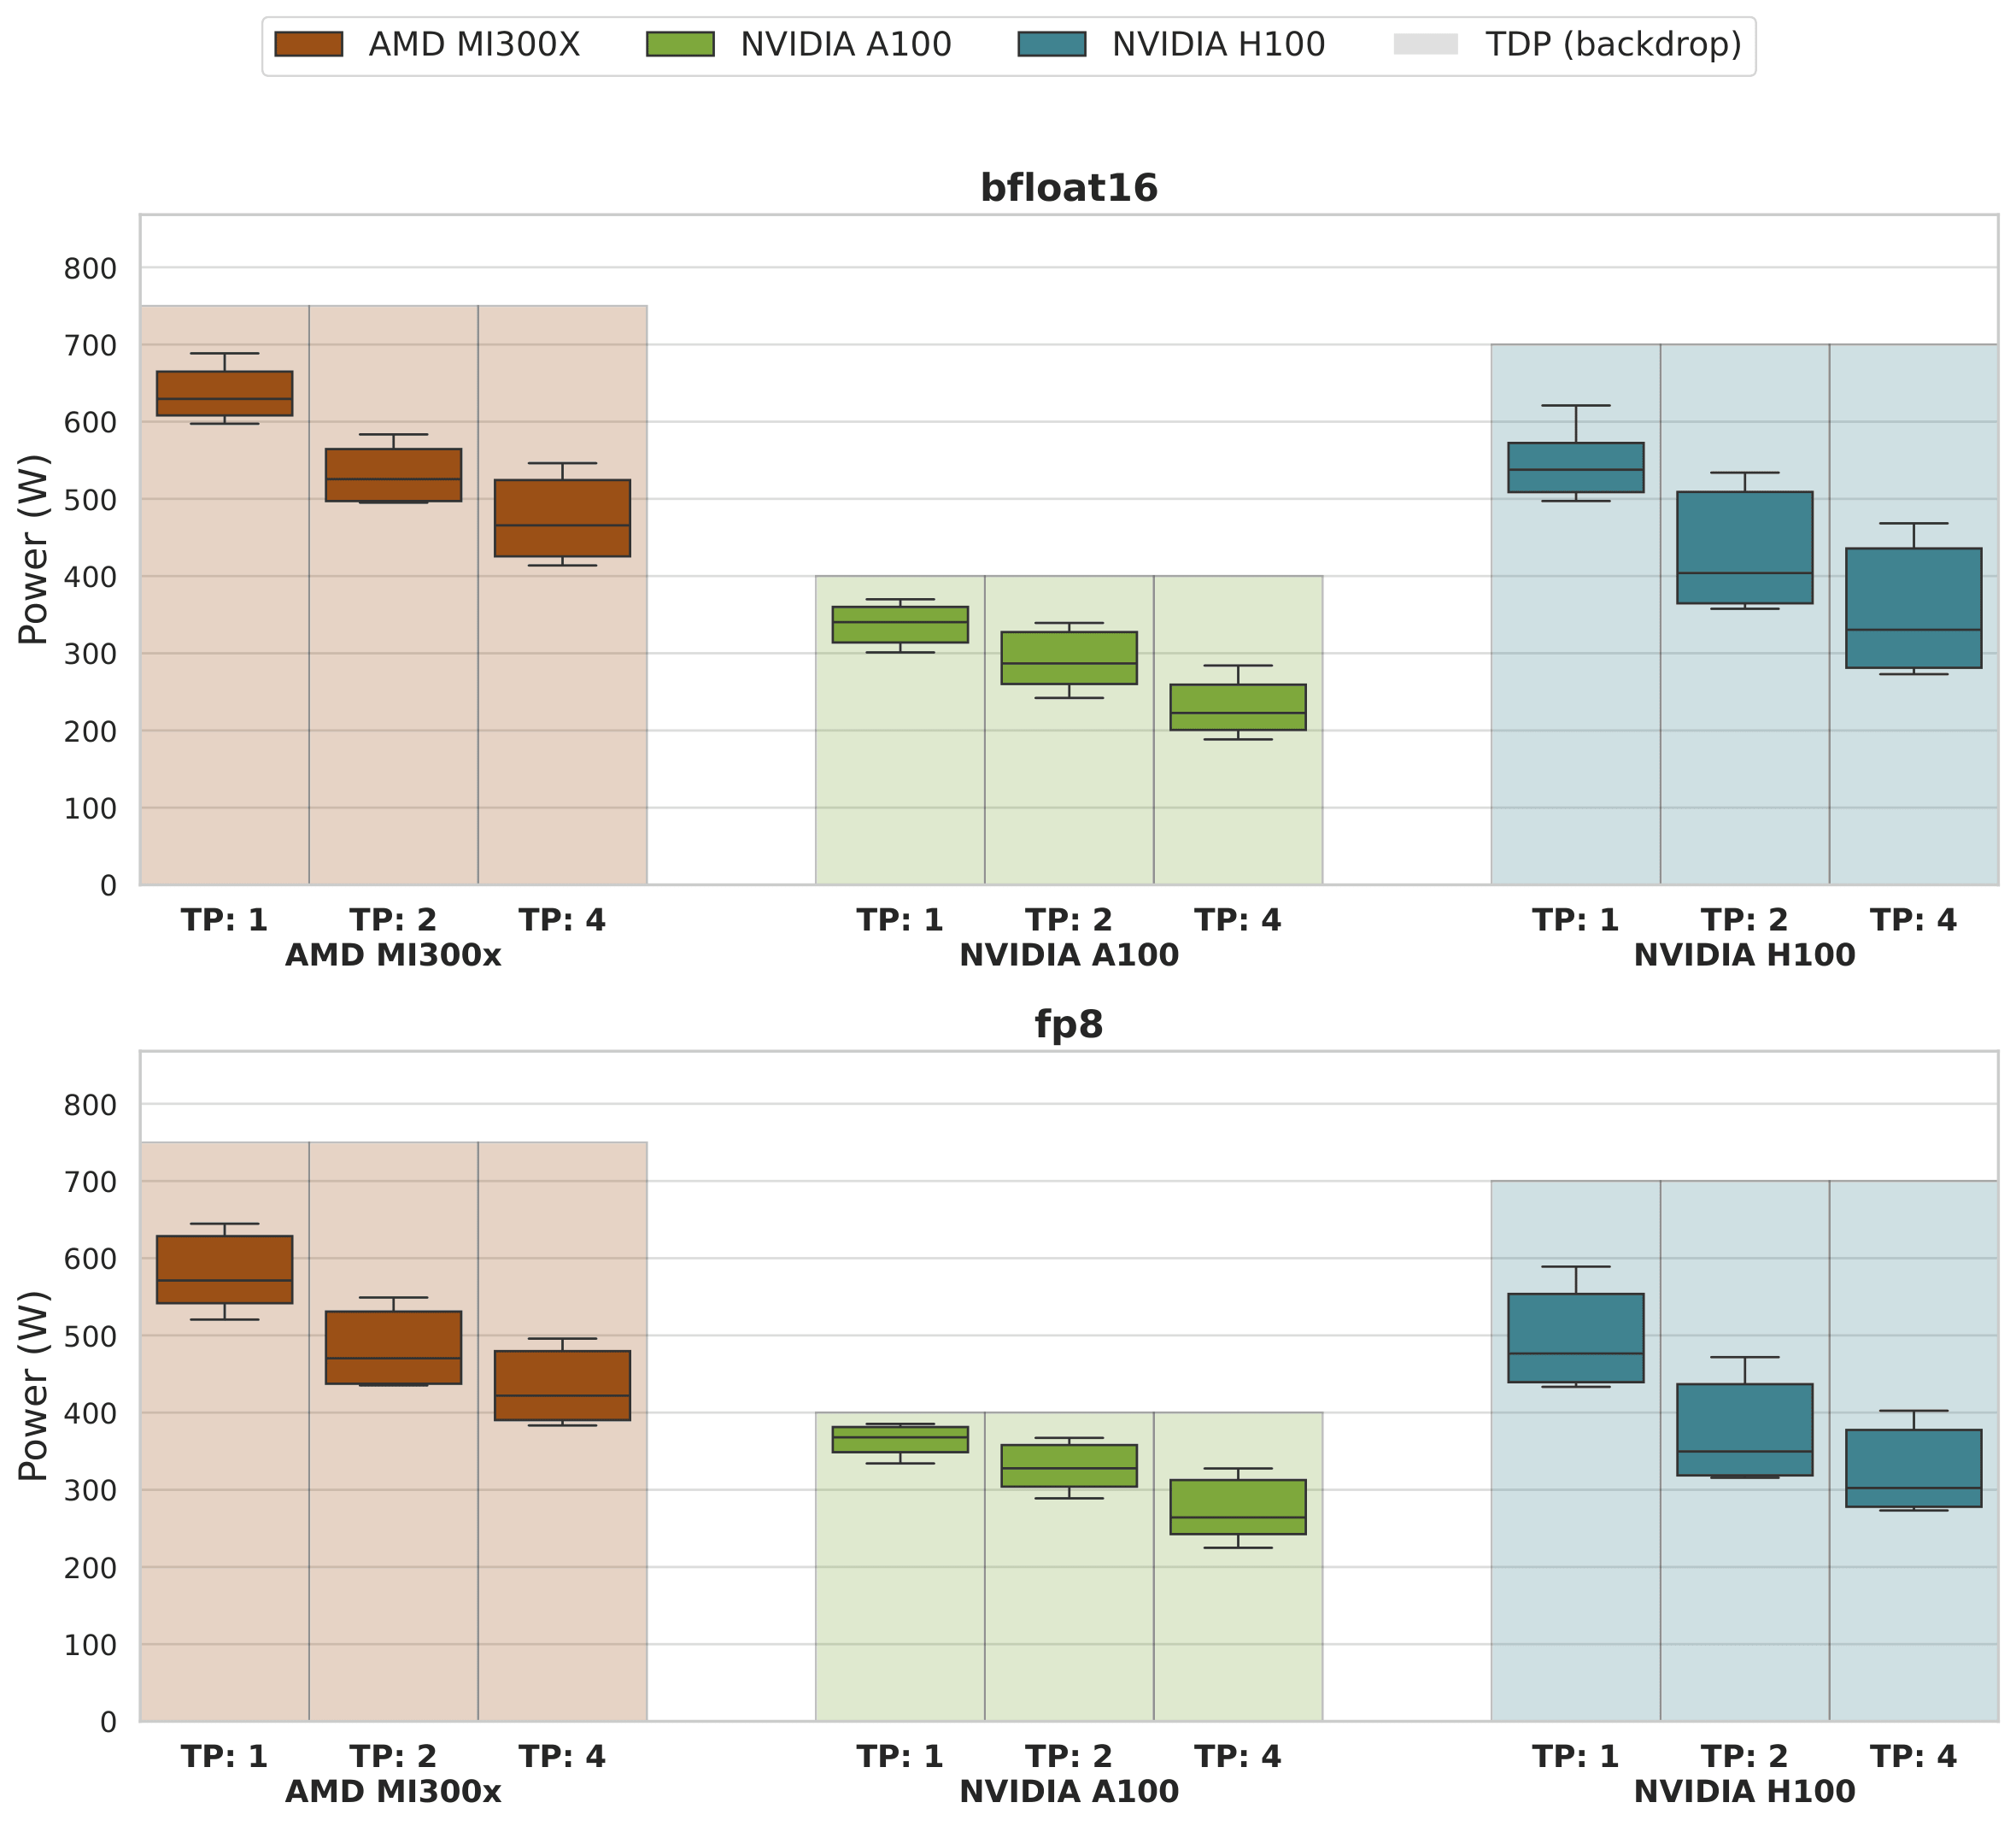
\includegraphics[width=0.95\columnwidth]{figs/efficiency_boxplot_merged_active_power_avg_bfloat16_fp8.png}
    \caption{Power consumption with Tensor Parallelism.}
    \tagpdfsetup{alttext={Power consumption with Tensor Parallelism.}}
    \label{fig:powbars}
\end{figure}

\subsection{Model Size  Scaling}
The second aspect of our analysis investigates how energy efficiency and performance evolve with increasing model size and sparsity. \ref{fig:scaling} presents the trends of four key metrics as the number of parameters increases. The trends across dense models are represented by solid lines, while dashed lines indicate the Mixture-of-Experts (MoE) model.

In Section~\ref{chap:results:sec:single}, we observe that dense models exhibit a linear increase in end-to-end latency and TTFT as model size grows, while throughput and energy efficiency decrease inversely—consistent with the behavior predicted by our performance model, consistently with what was discussed in Section \ref{chap:methods:sec:model}. This trend remains stable even when scaling to multi-GPU configurations with a fixed Tensor Parallel (TP) size.

When comparing different TP/DP configurations, we find that not all metrics scale uniformly under this weak-scaling setting. End-to-end latency and TTFT remain largely constant across TP configurations, whereas throughput and energy efficiency improve in smaller TP setups. Consequently, when considering the best attainable performance across configurations, we observe linear scaling in latency and TTFT, accompanied by an even more pronounced decline in throughput and energy efficiency as model size increases.

A distinct pattern emerges when analyzing Mixture-of-Experts (MoE) models (dashed lines in \ref{fig:scaling}). 
As discussed in \ref{chap:model:sec:moe}, Mixture-of-Experts models activate only a subset of their weights during inference, reducing the number of floating-point operations per forward pass from $2N$ to $2A$, where $N$ is the total number of parameters and $A$ is the number of active parameters. However, their memory load operations depend on the number of experts that are active at each level. In the case of a batch size of 1, loading operations also decrease from $N$ to $A$, while for larger batch sizes, most experts are loaded, resulting in a lower ideal speedup.

When observing experimental data, we can observe that, keeping constant hardware resources, MoE models consistently achieve higher performance and energy efficiency than dense models of comparable size. This demonstrates the effectiveness of the MoE architecture in scaling model parameters and accuracy while maintaining strong computational and energy efficiency. For example, Llama 4 Scout—with 109B total parameters—achieves 17\% higher throughput and 52\% better energy efficiency than the smaller Llama 3 70B on NVIDIA H100, by activating only 17B parameters during inference.
However, due to the impact of memory accesses, these gains are not strictly proportional to the degree of sparsity. On both NVIDIA H100 and AMD MI300X, Llama 4 Scout underperforms relative to Llama 3 Nemotron Super (49B), despite activating only 22B parameters.

\begin{figure}[h!]
    \centering
    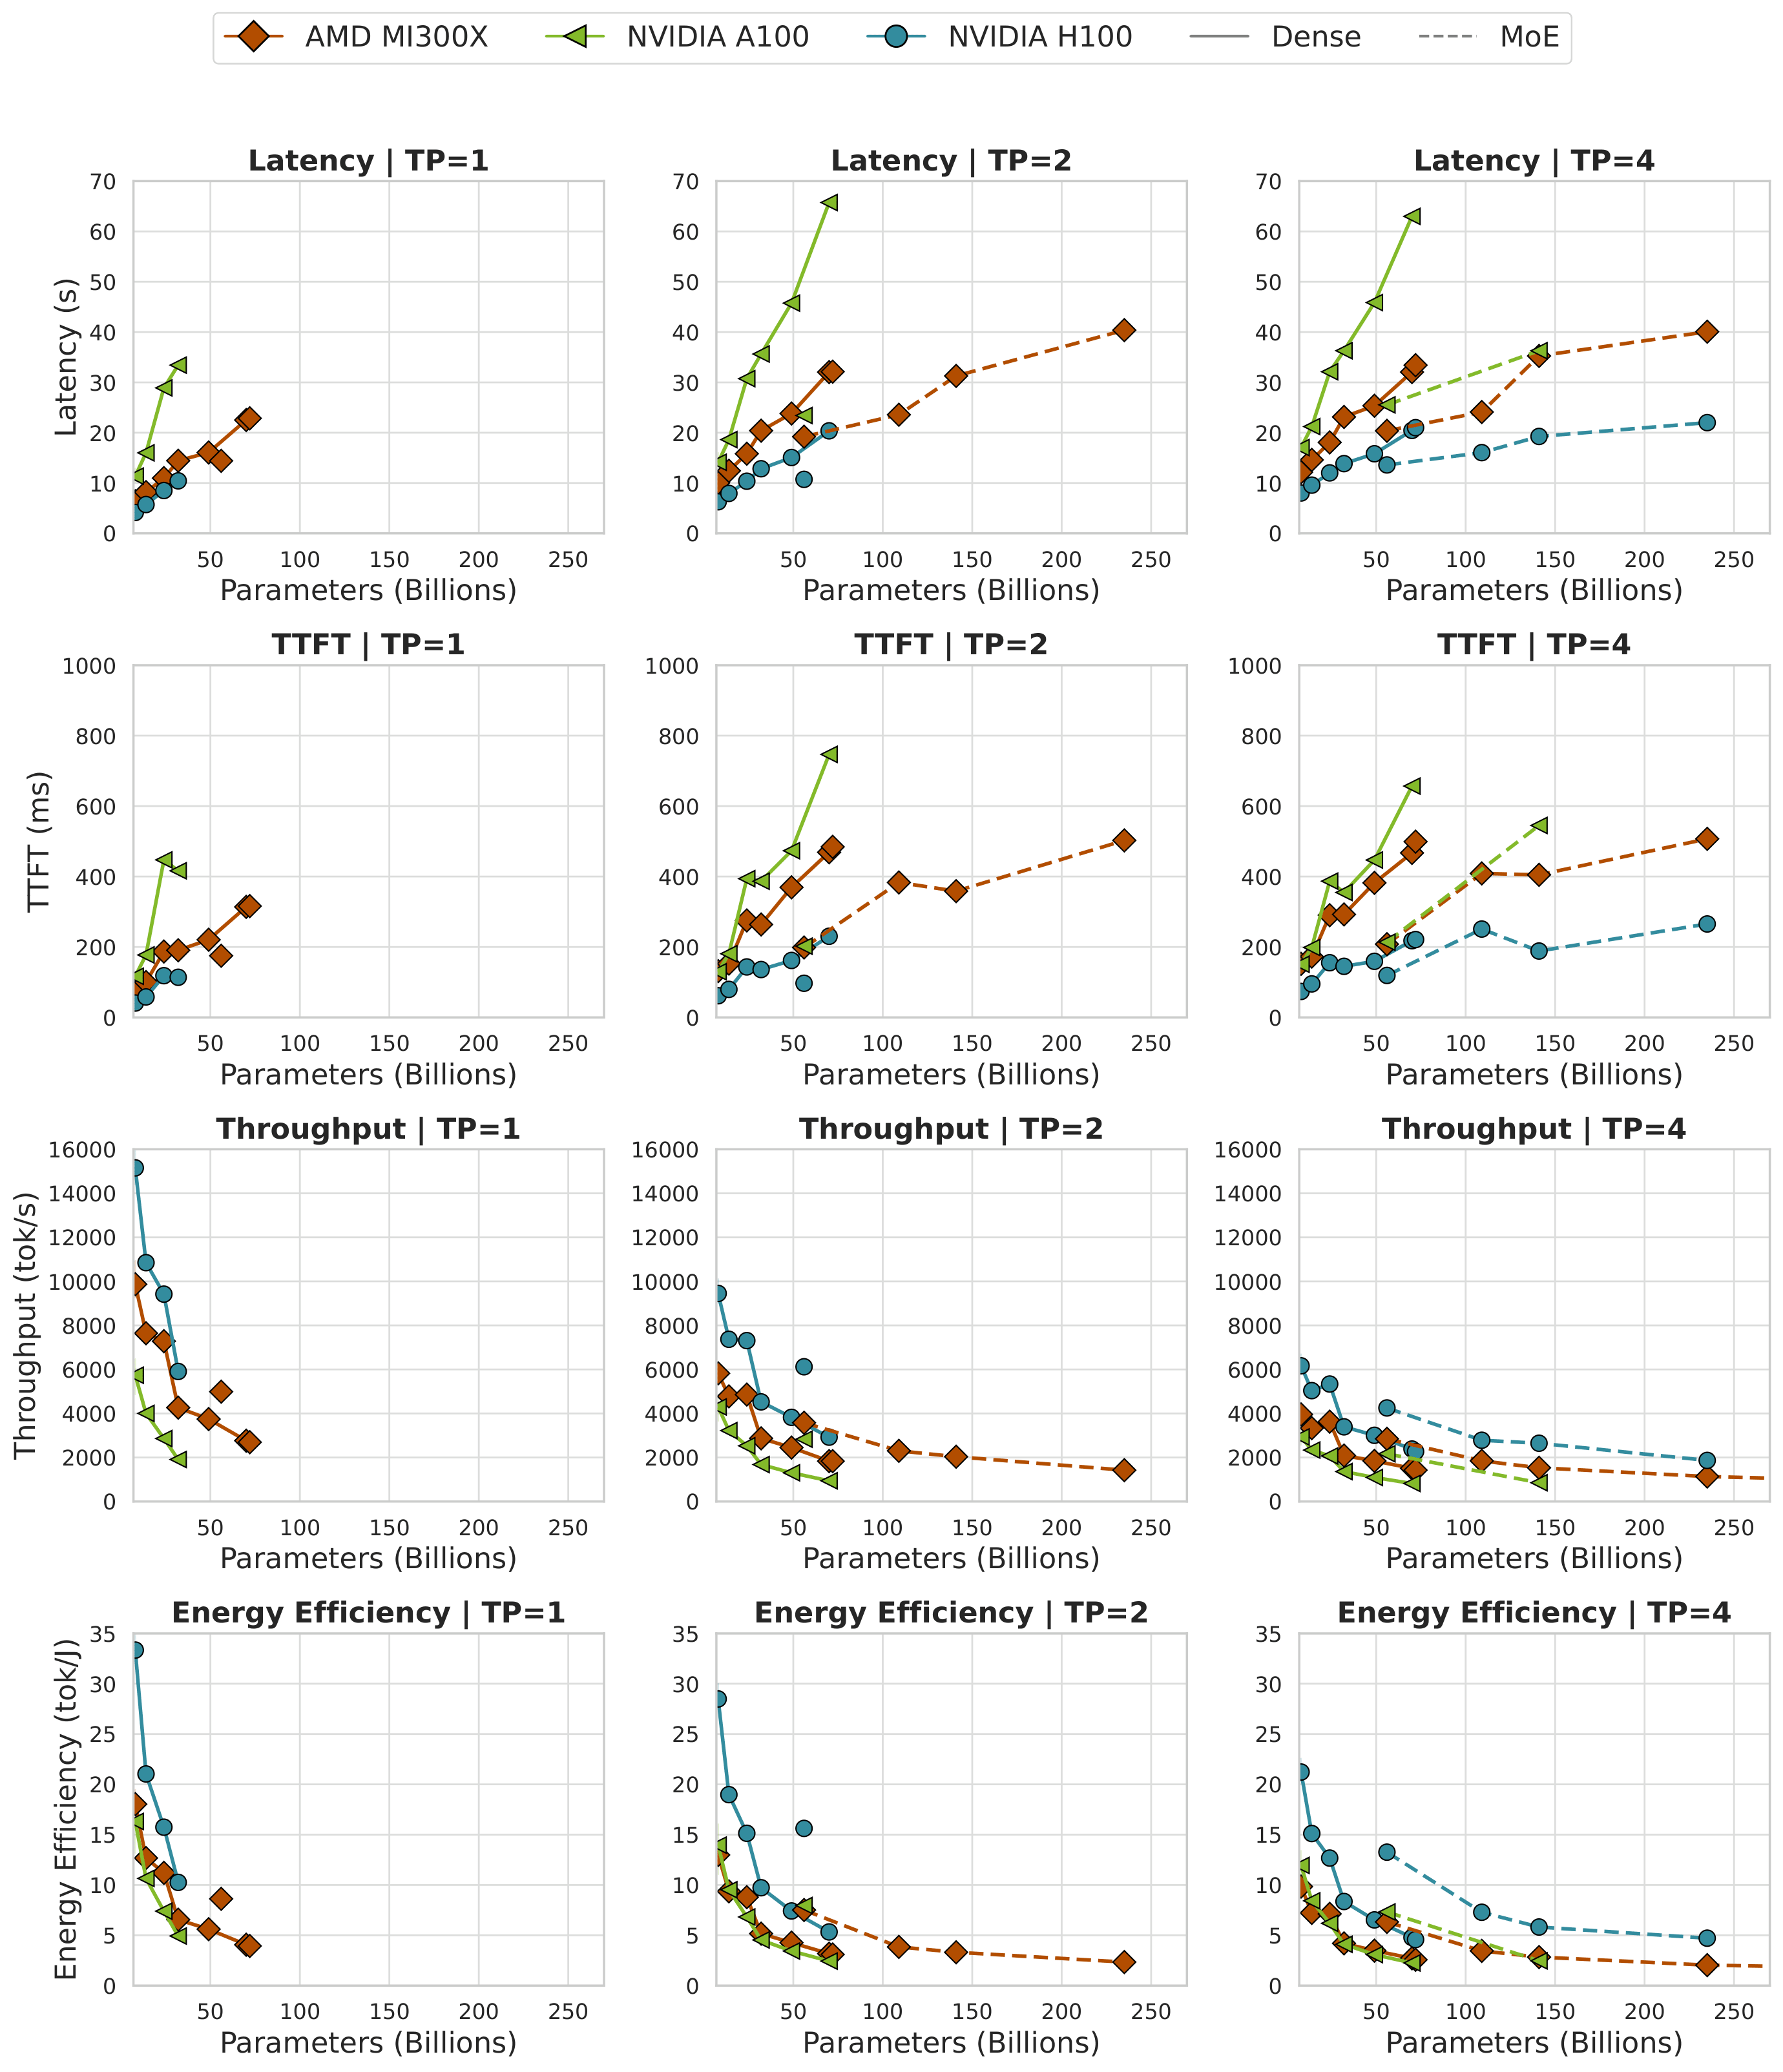
\includegraphics[width=\columnwidth]{figs/Combined_Metrics_NoBest.png}
      \caption{Scaling of performance metrics with model size.}
      \tagpdfsetup{alttext={Scaling of performance metrics with model size.}}
    \label{fig:scaling}
\end{figure}

\subsection{Tensor and Expert Parallelism}
In Section \ref{chap:background:sec:serving}, we introduced Expert Parallelism as an alternative approach to parallelizing inference in Mixture-of-Experts (MoE) models.
To evaluate its performance, we conduct a series of experiments comparing Tensor Parallelism and Expert Parallelism across four sparse large language models (LLMs). Each model is tested on both four NVIDIA H100 GPUs and four AMD MI300X GPUs, using both parallelization strategies and a range of batch sizes.

\begin{figure}[h!]
\centering
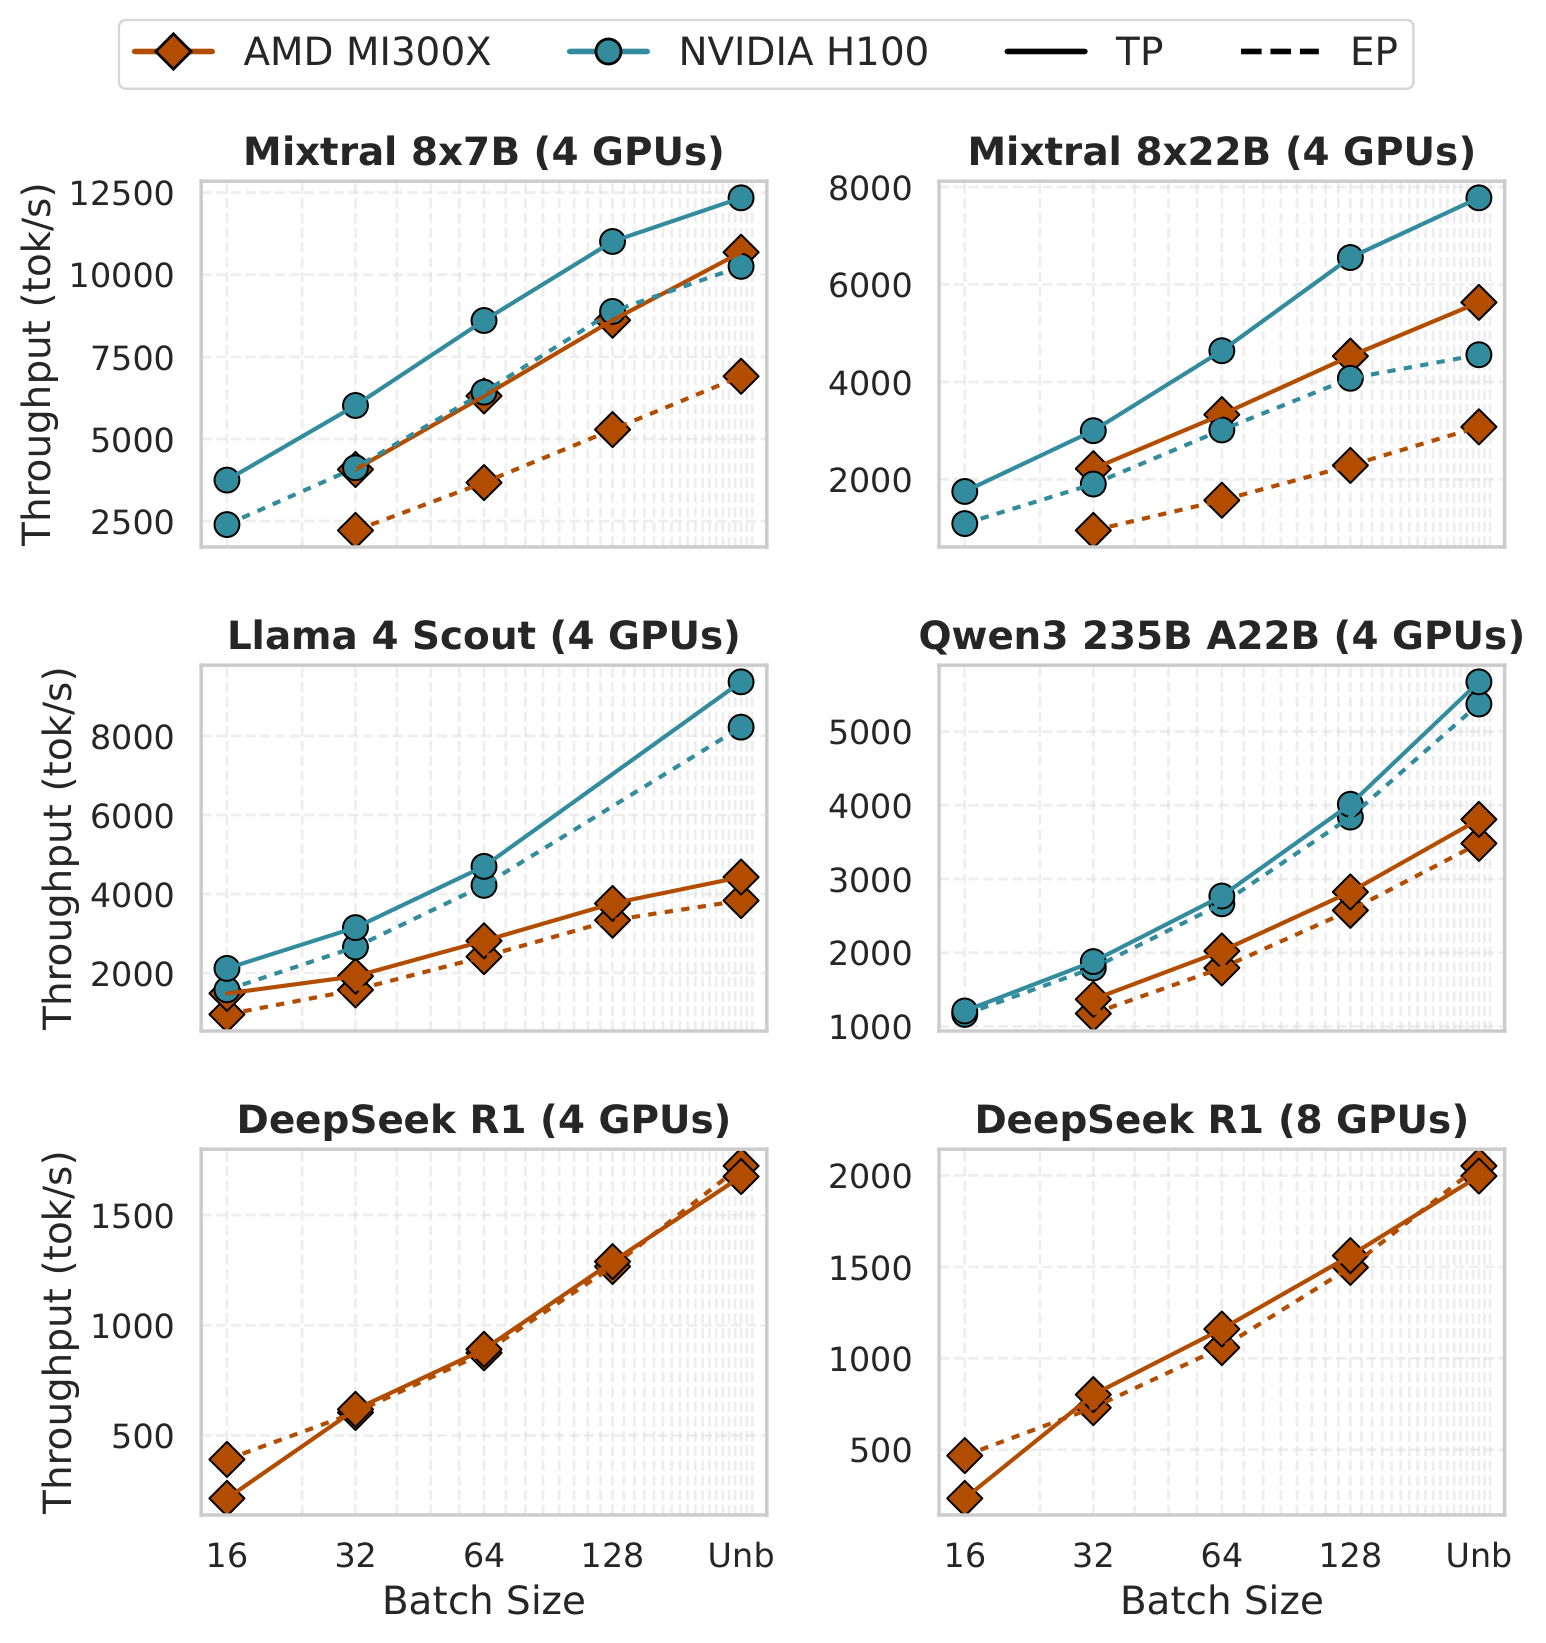
\includegraphics[width=0.75\columnwidth]{figs/combined_ep_tp.png}
\caption{Throughput using Tensor and Expert Parallelism.}
\tagpdfsetup{alttext={Throughput using Tensor and Expert Parallelism.}}
\label{fig:ep}
\end{figure}

At a first-level analysis, the results show that Tensor Parallelism consistently outperforms Expert Parallelism across all models, batch sizes, and hardware configurations—with one notable exception, which is discussed later.

A closer examination of model architectures reveals that the number of experts is a key factor driving this performance gap. Mixtral 8x22B, which employs eight experts, exhibits the largest advantage for Tensor Parallelism, achieving 61\% higher throughput on the H100 and up to 2.7 $\times$ higher throughput on the MI300X. For Llama 4 Scout (16 experts), Tensor Parallelism achieves 6\% higher throughput on the MI300X and 34\% higher throughput on the H100. Qwen3, with 128 experts, shows smaller improvements (16\% on MI300X and 4\% on H100). DeepSeek R1, however, deviates from this pattern due to its unique configuration—256 rooted experts plus one shared expert—which enables Expert Parallelism to match or exceed Tensor Parallelism at smaller batch sizes. At a batch size of 16, it achieves 82\% higher throughput with four GPUs and 100\% higher throughput with eight GPUs. As the batch size increases, this advantage diminishes, and both methods converge to similar performance levels.

The energy efficiency results largely reflect the throughput trends. Tensor Parallelism generally proves more energy-efficient, particularly for models with fewer experts. For instance, Mixtral 8x22B achieves twice the efficiency on the MI300X and a 60\% improvement on the H100, while Llama 4 Scout exhibits comparable gains. Qwen3 again shows marginal improvements (18\% on MI300X and 2\% on H100). DeepSeek R1 remains the exception: Expert Parallelism is more efficient at batch sizes of 16 or smaller, but Tensor Parallelism becomes more efficient as the batch size grows.


\subsection{GPU Model Comparison}
\ref{fig:heatmapbf16} and \ref{fig:heatmapfp8} report the throughput and energy efficiency of all the experimental results conducted with the three multi-GPU nodes in bfloat16 and FP8 precision, respectively.

Consistent with the findings presented in Section \ref{chap:results:sec:single}, the NVIDIA H100 achieves the highest throughput among all tested GPUs, in both bfloat16 and FP8 precisions. It is followed by the AMD MI300X, which consistently outperforms the NVIDIA A100. The performance gap between NVIDIA Hopper and AMD CDNA3 architectures, relative to NVIDIA Ampere, becomes more pronounced under FP8 quantization, as the newer architectures incorporate dedicated FP8 functional units that support W8A8 quantization, in contrast to W8A16 on Ampere.

In terms of energy efficiency, the results vary depending on the precision and model size. With bfloat16 precision, the NVIDIA A100 demonstrates higher efficiency than the AMD MI300X for models with fewer than 32B active parameters. However, when using FP8 quantization, the MI300X consistently exhibits superior efficiency. Across all configurations, the NVIDIA H100 maintains the highest overall efficiency at both precisions.

Memory capacity also plays a crucial role in determining performance. While both NVIDIA GPUs provide 80 GB of HBM memory, the AMD MI300X offers 192 GB, yielding two major advantages: it can accommodate larger models and requires smaller tensor parallel sizes for equivalent workloads. As discussed earlier, Tensor Parallelism introduces frequent all-gather operations that hinder performance, making lower tensor parallel sizes desirable.

When comparing performance under a fixed GPU budget (e.g., four GPUs), the MI300X often achieves higher throughput due to its larger memory capacity. This enables it to operate in pure data-parallel mode, avoiding the communication overheads inherent to high tensor parallel sizes on NVIDIA systems. For instance, with Llama 3.3 70B in bfloat16 precision, the MI300X achieves approximately 2017 tokens per second per GPU with a tensor parallel size of 1, resulting in a total throughput of 8068 tokens per second across four GPUs. In contrast, the NVIDIA H100 reaches 7634 tokens/s under the same configuration but requires a tensor parallel size of 4. A similar pattern emerges for Qwen2 72B in bfloat16 precision.

\section{Dataflow Accelerators Experiments}
\label{chap:results:sec:dsa}

Finally, we analyze LLM inference performance and energy efficiency of two state-of-the-art dataflow AI accelerators (Cerebras CS3 and Sambanova SN40L), comparing their results with NVIDIA A100 and NVIDIA H100 GPUs.
To do so, we evaluate two Llama models of different sizes: Llama 3.1 8B and Llama 3.3 70B.

For Llama 3.1 8B, Cerebras, and SambaNova provide pre-compiled artifacts that support batch sizes from 1 to 8, so we evaluate AI accelerators only within this range. In contrast, for GPUs, we test batch sizes from 1 to 128. GPU results are obtained using single-GPU inference, whereas the dataflow-accelerated systems use their full hardware configurations: one WSE for Cerebras and sixteen RDUs for SambaNova.

The larger 70B model instead is tested using 4 GPUs with Tensor parallelism on the GPU nodes and 16 RDUs on the SN40L machine. The Cerebras CS3 does not support single-node inference for this model, as its framework loads all the model weights into scratchpad memory (44 GB/WSE3), which is not capable of holding Llama 3.3 70B in bfloat16 precision (140 GB).

\subsection{Performance Comparison Across Batch Sizes}

\begin{figure}[h!]
    \centering
    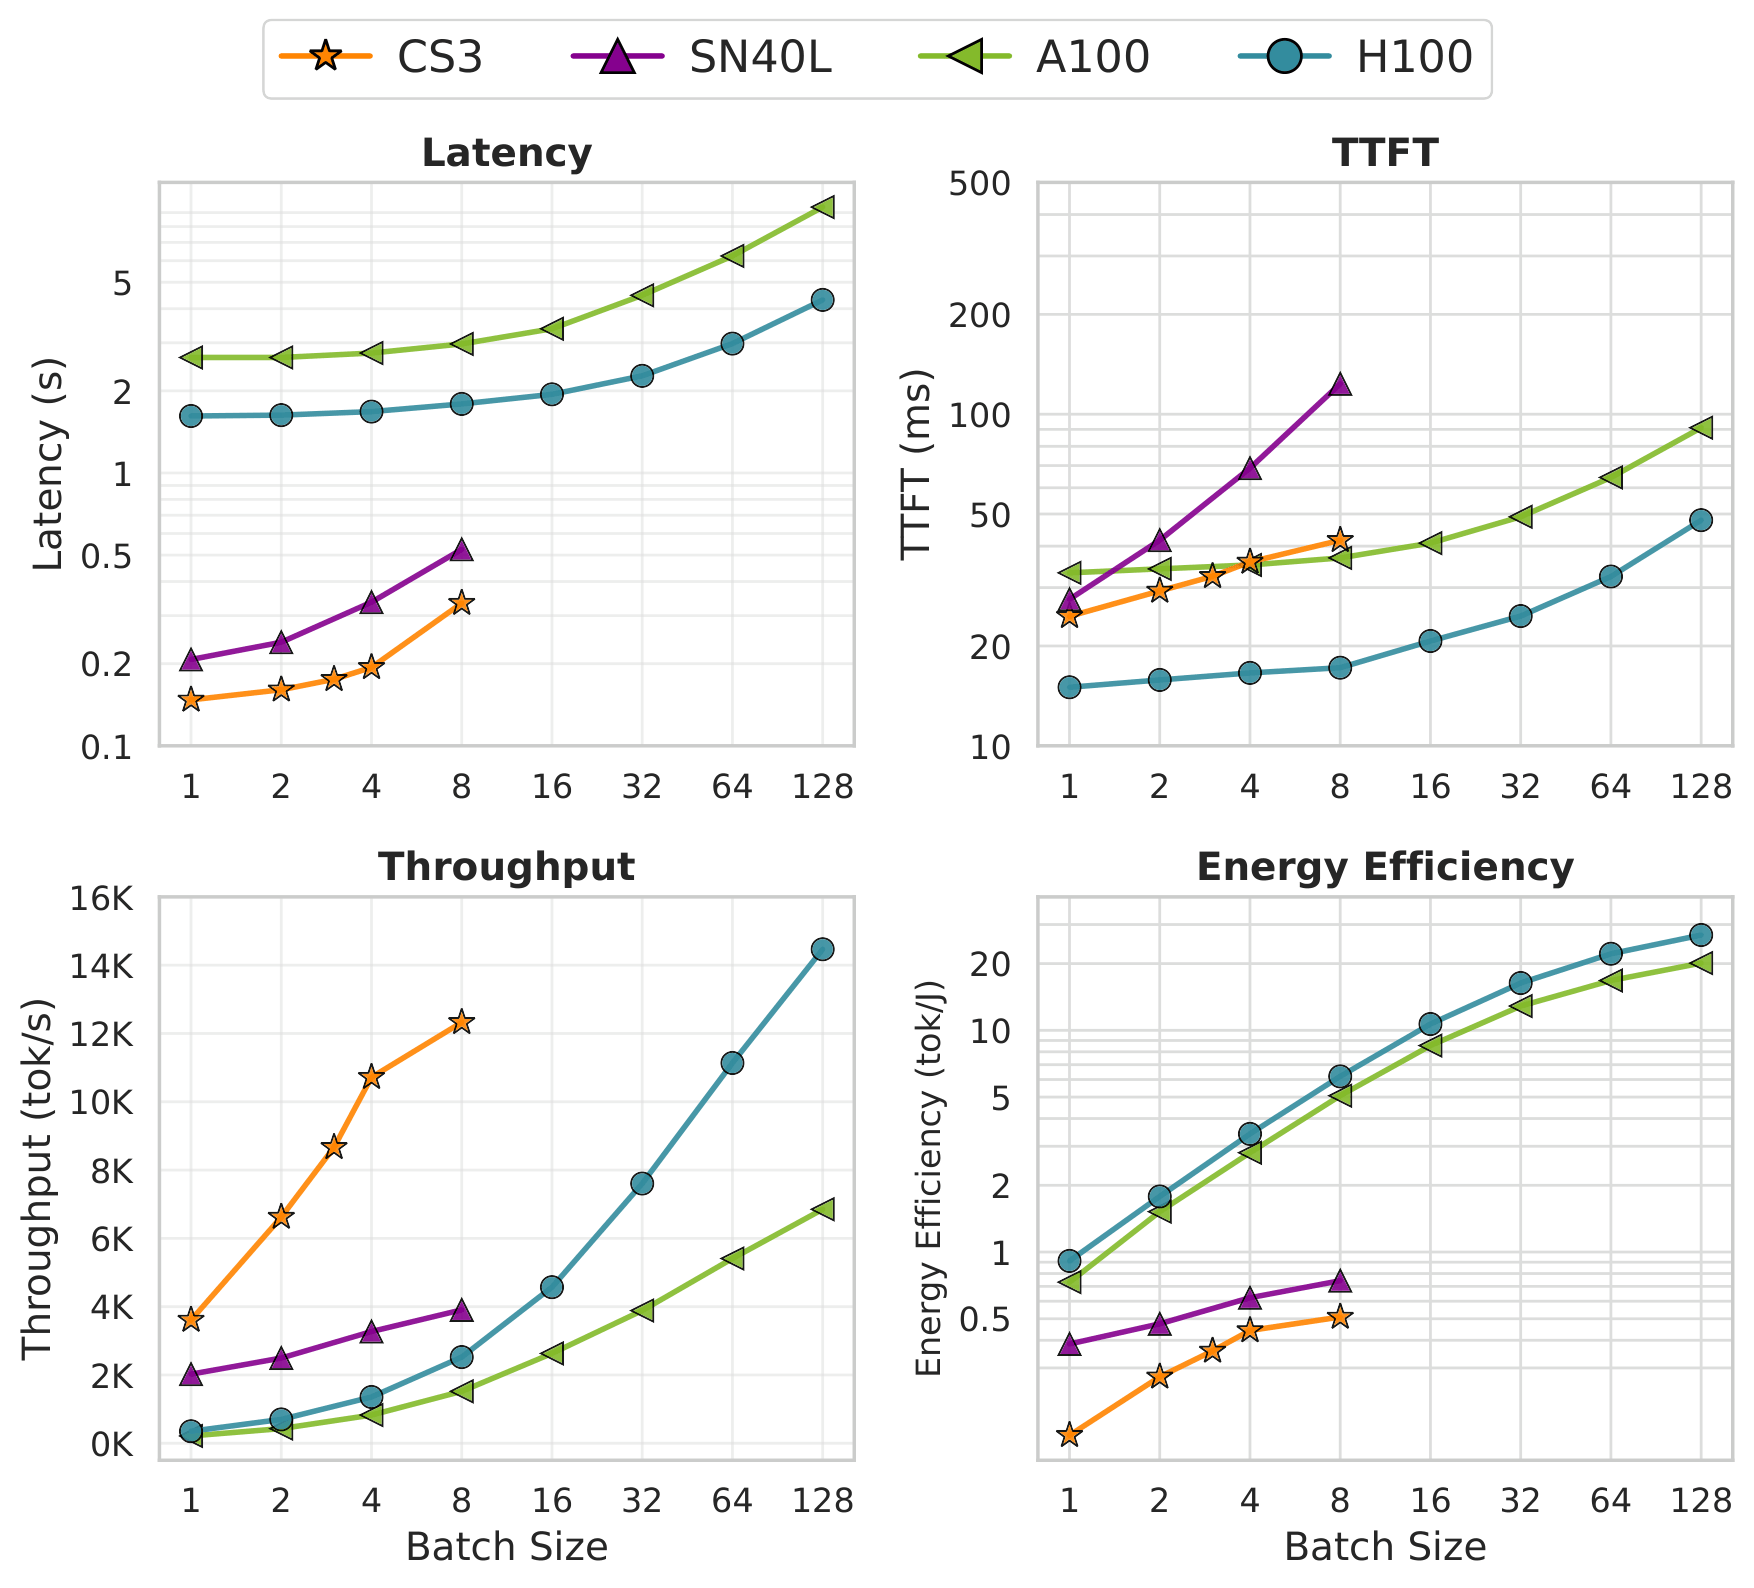
\includegraphics[width=0.8\columnwidth]{figs/testbeds_8B.png}
    \caption{Performance and energy efficiency of Llama 3.1 8B inference across AI accelerators.}
    \tagpdfsetup{alttext={Performance and energy efficiency of Llama 3.1 8B inference across AI accelerators.}}
    \label{fig:testbeds8}
\end{figure}

\ref{fig:testbeds8} and~\ref{fig:testbeds70} present the performance and energy-efficiency results for GPUs and dataflow accelerators running Llama~3.1~8B and Llama~3.3~70B, respectively, reporting four key metrics that highlight the differences in performance between GPUs and dataflow accelerators.

\begin{figure}[h!]
    \centering
    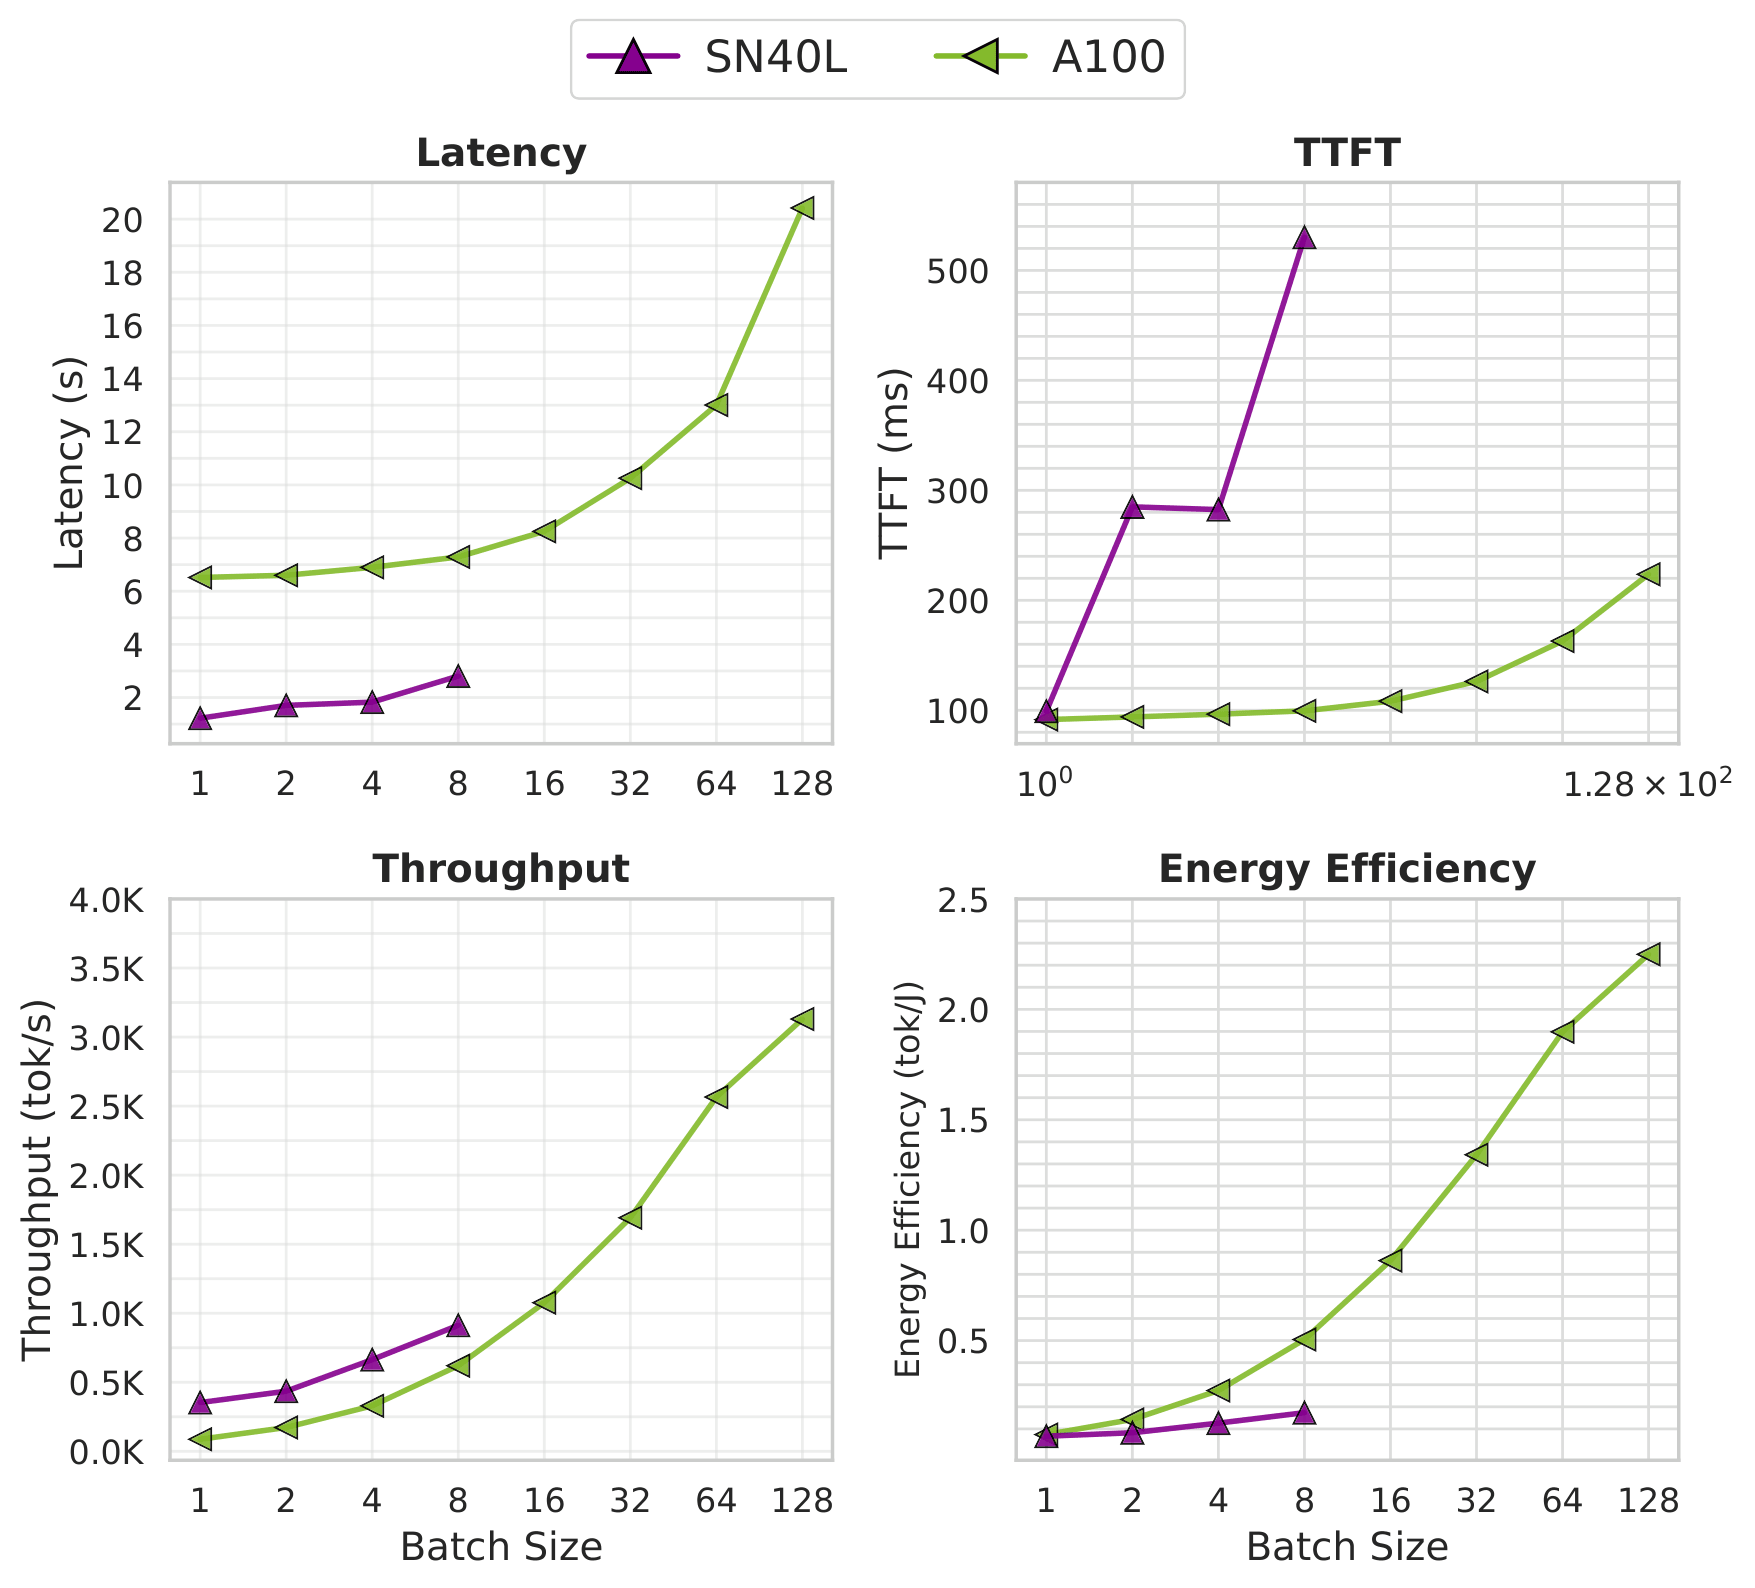
\includegraphics[width=0.8\columnwidth]{figs/testbeds_70.png}
      \caption{Performance and energy efficiency of Llama 3.3 70B inference across AI accelerators.}
    \tagpdfsetup{alttext={Performance and energy efficiency of Llama 3.3 70B inference across AI accelerators.}}
    \label{fig:testbeds70}
\end{figure}

Our experimental data clearly demonstrate how different architectures impact computation. As extensively discussed in Section \ref{chap:methods:sec:model}, LLM inference performance is directly related to the latency of the forward pass, which is composed of two parts: the latency of the computation and the latency of memory loading operations. GPUs host the model weights in off-chip HBM memories, which provide a bandwidth of approximately 1 to 5 TB/s. Dataflow accelerators, on the other hand, rely on local scratchpad memories, which are up to four orders of magnitude faster than GPUs, aiming to alleviate the impact of memory reads on the overall performance.
fi
At first, we observe that within their supported batch sizes, dataflow machines achieve markedly lower latency and substantially higher throughput than GPUs. The most pronounced improvement occurs at batch size 1, where the computation is the most memory-bound.
NVIDIA A100 reaches 215 tokens/s, compared to 3609 tokens/s (16.8$\times$) on the Cerebras CS3 and 2024 tokens/s (9.41$\times$) on the SambaNova SN40L.
The SamabaNova SN40L also outpaces GPUs with Llama 3.3 70B, achieving 353 tokens/s at a batch size of 1, compared to 88 tokens/s (4.01$\times$) obtained with 4 NVIDIA A100s working with Tensor Parallelism.

Increasing the batch size also increases the operational intensity $OI$, allowing GPUs to progressively close the GAP. In their supported batch size range (1-8), dataflow accelerators still outpace GPUs in terms of latency and throughput. However, due to the larger impact of computation on overall latency, we notice that dataflow accelerators display notably steeper increases in end-to-end latency and TTFT compared to those of GPUs.

Another observation regards peak throughput.
We established that dataflow machines exhibit superior performance at small batch sizes, but we also assessed the fact that their maximum supported batch size is substantially lower, sometimes due to a lack of compile artifacts for larger batch size configurations. In fact, both Cerebras and SambaNova provide precompiled artifacts that allow running at fixed batch sizes of 1 to 8. vLLM, on the other hand, handles batch sizes dynamically, allowing us to test batch sizes up to 128.
In an offline scenario, where the maximum achievable throughput using the optimal batch size is the only relevant performance metric, we observe that the capacity of GPUs to scale to larger batch sizes allows them to narrow the performance gap in terms of peak throughput. Cerebras, at a batch size of 8, produces 12327 tokens/s, outperforming both the NVIDIA A100 and the AMD MI300x. However, it is still outperformed by the NVIDIA H100 at a batch size of 128, which achieves 14,455 tokens/s. The SambaNova SN40L instead peaks at 3,907 tokens/s with a batch size of 8.
From this, we can conclude that the performance benefits of modern dataflow accelerators are noticeable, particularly in online settings with low batch sizes and a limited number of requests per node. In offline batch-inference jobs, the dynamic batch size supported by GPUs makes this architecture still preferred.

This causes dataflow accelerators to dominate online inference scenarios with a reduced number of concurrent requests, while in an online scenario where the only requirement is high throughput, they lose their competitive advantage in terms of raw performance.

\subsection{Comparison of ITL and TTFT}

\begin{figure}[h!]
    \centering
    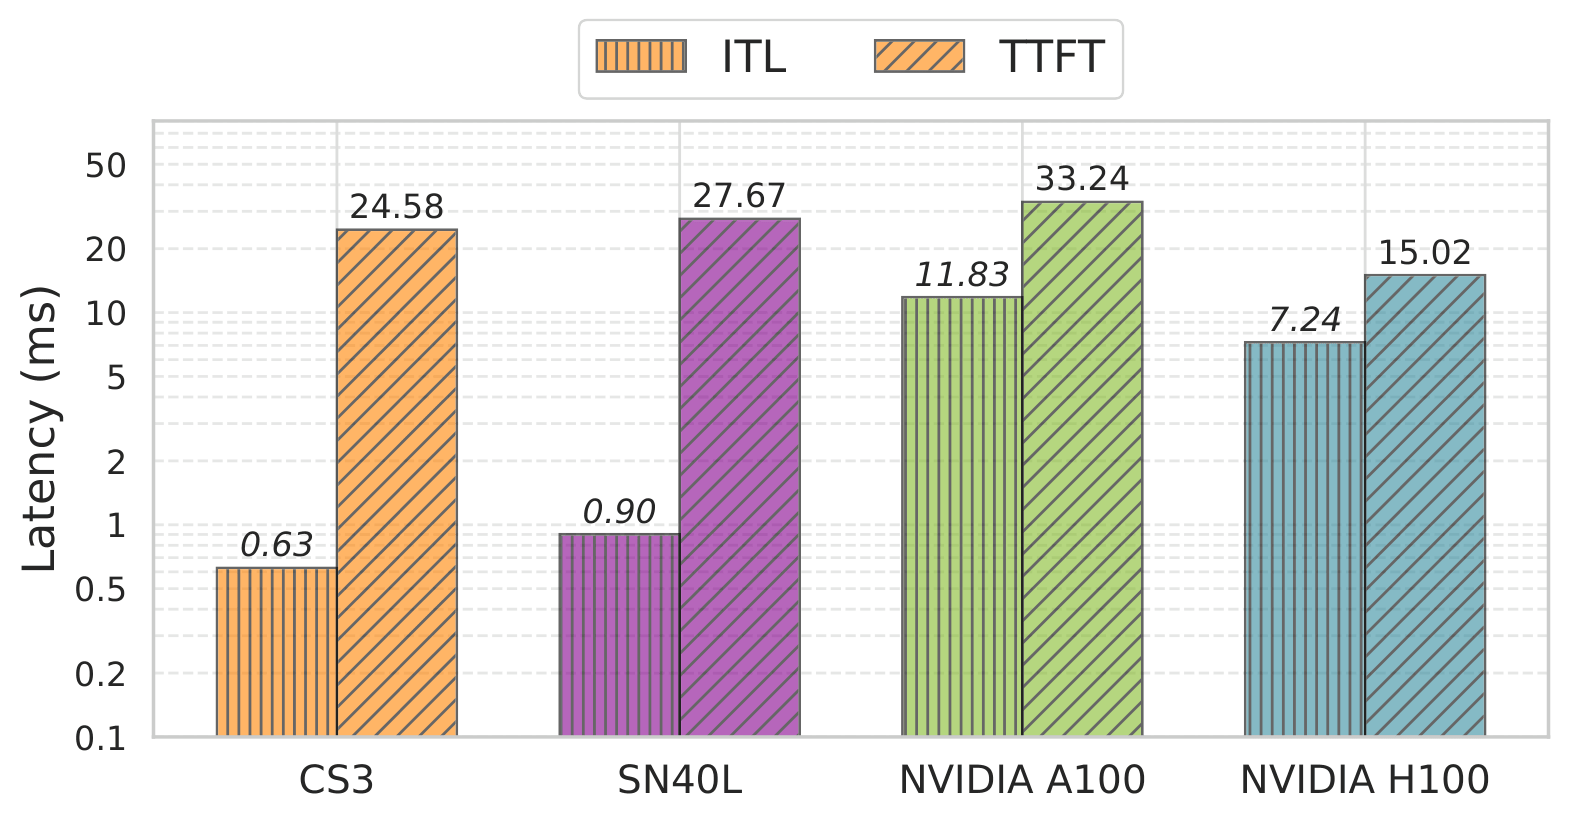
\includegraphics[width=\columnwidth]{figs/itl_ttft.png}
      \caption{Time-to-first-token (TTFT) and Inter Token Latency (ITL) of GPUs and dataflow accelerators.}
      \tagpdfsetup{alttext={Time-to-first-token (TTFT) and Inter Token Latency (ITL) of GPUs and dataflow accelerators.}}
    \label{fig:itl-ttft}
\end{figure}

Digging further into the impact of memory bandwidth on computation, we compare the ITL and TTFT across the different architectures. As discussed in \ref{chap:methods:sec:metrics}, TTFT is the average latency of the compute-bound prefill phase, while ITL indicates the average latency of the memory-bound decode phase.
\ref{fig:itl-ttft} displays TTFT and ITL of Llama 3.1 8B at batch size 1.
It allows us to observe once again how the benefit of dataflow accelerators stems from their improved data locality and memory bandwidth. In fact, while the TTFT of the SambaNova SN40L and the Cerebras CS3 is comparable with that of NVIDIA GPUs, the ITL is faster by one order of magnitude. Precisely, the Cerebras CS3 achieves an 18.8 $\times$ lower ITL compared to the NVIDIA A100, while SambaNova shows a 13.1 $\times$ improvement. A similar pattern appears when comparing Llama 3.3 70B performance: the SambaNova SN40L achieves slower TTFT compared to 4 NVIDIA A100 (99 ms compared to 91 ms), while having a 5.18 $\times$ shorter ITL (5.6 ms compared to 29 ms).

\subsection{Energy Efficiency}
\begin{figure}[H]
    \centering
    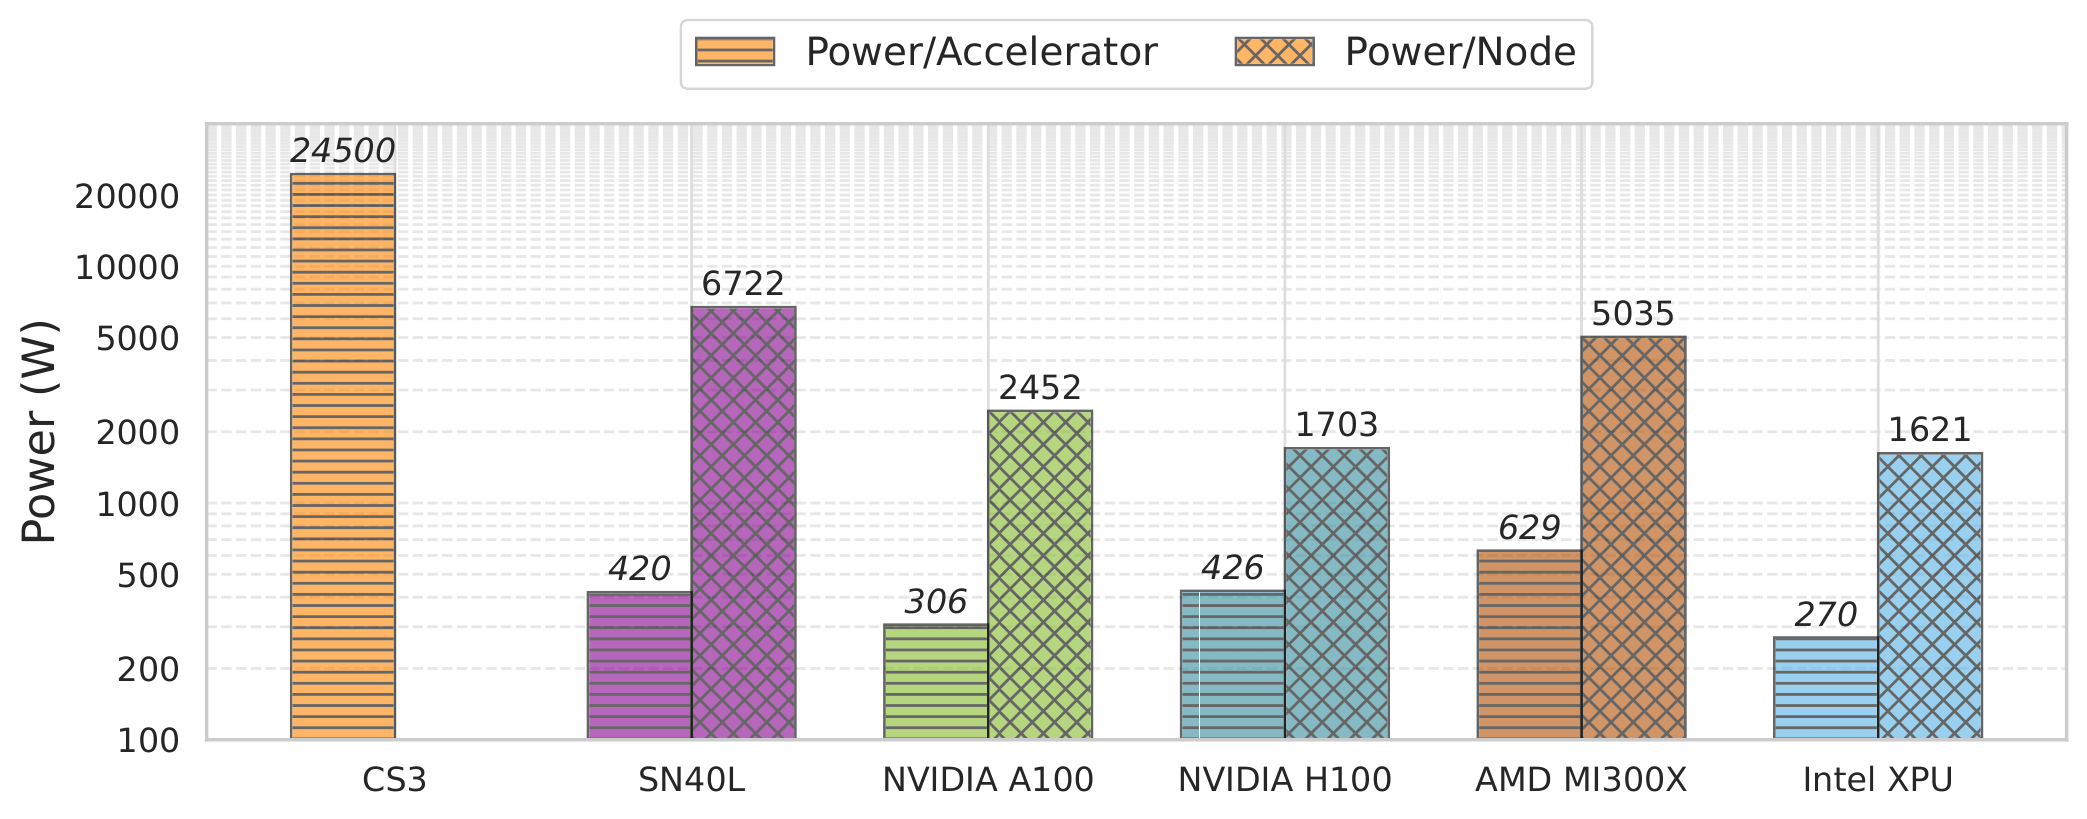
\includegraphics[width=\columnwidth]{figs/power_testbeds.png}
      \caption{Power consumption of GPUs and AI accelerators.}
      \tagpdfsetup{alttext={Power consumption of GPUs and AI accelerators.}}
    \label{fig:power}
\end{figure}

Finally, we analyze energy efficiency. To benefit from reduced memory bandwidth, dataflow accelerators employ a substantially larger number of cores that store weights and activations in their local memory, resulting in higher overall power consumption. As shown in \ref{fig:power}, to run Llama 3.1 8B in half precision, Cerebras CS3 draws around 24500W of power, and the SambaNova SN40L uses 420W per RDU, for a total of 6722W for the whole SN40L-16R system. Compared to the multi-GPU nodes, we observe that for the same model at a batch size of 16, GPUs use between 306 W and 630W of power.

For this reason, at no batch size, dataflow accelerators exhibit competitive energy consumption compared to GPUs (as shown in \ref{fig:testbeds8} and \ref{fig:testbeds70}), even though they display substantially better performance.

For this reason, we can conclude that a trade-off exists between low-latency, throughput, and energy efficiency among different types of accelerators.

\chapter{Related Work}
\label{chap:related}

As large language model (LLM) inference becomes an increasingly significant contributor to datacenter energy consumption, research on performance and energy efficiency has grown substantially. This section surveys the most relevant work across GPU-based LLM inference, Mixture-of-Experts (MoE) model evaluation, and dataflow accelerator performance.

\section{LLM Inference on GPUs}

Chitty-Venkata et al. ~\cite{LLMInfbench} provides one of the most comprehensive evaluations of modern LLM inference and serves as the primary point of reference for this thesis. The benchmark examines several major dimensions of inference performance.

First, it evaluates a broad set of model architectures, covering both dense and Mixture-of-Experts models from the LLaMA, Mistral, and Qwen families. The comparison spans two parameter scales: 7B models (LLaMA-2-7B, LLaMA-3-8B, Mistral-7B, Qwen-2-7B) and 70B–72B models (LLaMA-2-70B, LLaMA-3-70B, Mixtral-8x7B, Qwen-2-72B).

Second, the study analyzes token-generation parameters, including input length, output length, and batch size, assessing how these factors affect both latency and throughput.

Third, it compares performance across multiple hardware platforms, including NVIDIA A100, H100, and GH200 GPUs, as well as SambaNova SN40L and Habana Gaudi2 dataflow accelerators.

Fourth, it measures performance across different inference frameworks, such as vLLM, DeepSpeed-MII, llama.cpp, and TRT-LLM, enabling a cross-stack comparison.

Finally, the benchmark studies the effect of several optimization techniques, including KV caching, quantization, and other runtime-level optimizations.

Performance is characterized using key metrics: time to first token (TTFT), inter-token latency (ITL), throughput (input and output tokens multiplied by batch size per unit latency), and performance per watt based on average power consumption.

Building upon this work, our study places a stronger emphasis on energy efficiency and multi-GPU scaling behavior, while also extending the evaluation to dataflow accelerators.

A complementary study from the same authors ~\cite{chitty2025moe} analyzes the performance of several Mixture-of-Experts LLMs and vision–language models (VLMs), focusing on the architectural factors that shape their inference characteristics.


\section{Energy Efficiency of LLM Inference}

Several works focus specifically on the energy usage of LLM inference on modern GPUs.  

Fernandez et al.~\cite{fernandez2025energy} examine the impact of optimizations such as continuous batching, kernel compilation, and PagedAttention.  

Wilhelm et al.~\cite{wilhelm2025beyond} analyze test-time compute strategies—including majority voting and Chain-of-Thought prompting—exploring the efficiency–accuracy trade-off.  

Wilkins et al.~\cite{wilkins2024offline} characterize energy and performance across seven LLMs running on NVIDIA A100 GPUs.  

Dynamo-LLM~\cite{stojkovic2025dynamollm} benchmarks six models on H100 GPUs under varied tensor-parallel configurations, with a focus on multi-GPU scaling efficiency.  

Other works investigate GPU frequency scaling as a mechanism to improve the performance–efficiency balance~\cite{maliakel2025investigating, kakolyris2024slo, stojkovic2024towards}.

Unlike these studies, our analysis jointly evaluates performance and energy efficiency across modern GPUs from multiple vendors (NVIDIA, AMD, and Intel), as well as across three dataflow AI accelerators, yielding new insights into LLM inference across diverse deployment environments.

\section{Dataflow Accelerators}

Several studies have examined the performance of dataflow accelerators.  
Emani et al.\ published two influential works~\cite{Emani2021, Emani2022}.  
The first compares emerging AI accelerators—including the SambaNova SN10-8R, Cerebras CS-2, Graphcore IPU M-2000, and GroqNode—against the NVIDIA A100 GPU. The workloads include deep learning primitives, MLPerf benchmark models (ResNet, U-Net, BERT), and scientific machine learning applications. This initial study characterizes execution time and computational throughput but does not measure power consumption.

The second study evaluates LLM inference and training performance across five dataflow accelerators, comparing them against NVIDIA A100 and AMD MI250 GPUs using two LLMs (GPT-2 XL and GenSLM).

Ferdaus et al.~\cite{ferdaus2025evaluating} further examine BERT training and inference performance, as well as energy efficiency, on four dataflow accelerators, again comparing the results with those of the NVIDIA A100.  

While these studies form the foundation of our analysis, they primarily evaluate older LLMs that no longer reflect the current state of the art. Our work, therefore, updates and extends this line of research using modern LLM architectures and contemporary accelerator platforms.

\section{MLPerf}

MLPerf is the most widely used benchmark suite for evaluating the performance of systems on machine learning workloads. Introduced in 2018 by the MLCommons organization—a consortium formed by industry and academic partners—it provides standardized, open, and reproducible methodologies for comparing hardware and software platforms. The suite comprises three major components: MLPerf Training, MLPerf Inference, and MLPerf Power.

MLPerf Training~\cite{mattson2020mlperf} focuses on end-to-end training performance, reporting the time required for a system to train a model to a specified target accuracy. The workloads correspond to the same models used in the Inference benchmark, enabling consistent cross-comparisons between training and inference performance.

MLPerf Inference~\cite{reddi2020mlperf} evaluates the performance of systems running pre-trained machine learning models across tasks such as image classification, object detection, natural language processing, and recommendation. It measures both latency and throughput across a variety of deployment scenarios, including datacenter, edge, and mobile environments. To capture real-world usage conditions, MLPerf Inference defines four load-generator scenarios. The single-stream scenario processes a single request stream with batch size one, emphasizing strict latency constraints. The multi-stream scenario also uses a single stream but with a fixed arrival pattern and batch sizes greater than one. The server scenario models unpredictable request arrivals across multiple streams while maintaining batch size one. Finally, the offline scenario captures throughput-oriented batch processing where all inputs are available in advance, and latency is not a limiting factor.

For language workloads—those most relevant to our study—the current MLPerf Inference benchmark includes six LLMs: BERT-Large, GPT-J, Llama2-70B, Llama3-405B, Mixtral-8x7B, and DeepSeekR1. These models span parameter sizes from 340M to 670B and include both dense and Mixture-of-Experts architectures, enabling comparisons that reflect contemporary large-scale LLM deployments.

MLPerf Power~\cite{Tschand2024} provides the standardized methodology for measuring energy consumption during MLPerf Training and Inference workloads. The guidelines emphasize that commonly used metrics such as Thermal Design Power (TDP) and Power Supply Unit (PSU) ratings do not accurately represent real system-level power usage, as they incorporate significant safety margins and fail to capture dynamic fluctuations in power draw. MLPerf Power, therefore, offers more precise measurement requirements to support reliable assessments of energy efficiency across diverse hardware platforms.
\chapter{Conclusion}
\label{chap:conclusion}


In this thesis, we make the following contributions:

\begin{itemize}
    \item We present, in Chapter~\ref{chap:hardware}, a detailed survey of contemporary LLM inference accelerators and analyze the architectural challenges that shape modern hardware design for large-scale inference.

    \item We develop a performance benchmark that systematically evaluates the main determinants of LLM inference performance, including model size and sparsity, batch size, quantization strategies, and multi-GPU execution techniques.

    \item We conduct a comprehensive evaluation of a diverse set of accelerators, including six GPUs and two dataflow systems. For all platforms, we measure both performance and energy efficiency, addressing an important gap in prior work, which has predominantly focused on performance alone.

    \item We provide a principled analysis of dataflow accelerator behavior in LLM inference, clarifying how batch size influences throughput, latency, and energy efficiency, and dispelling common misconceptions regarding their performance characteristics.
\end{itemize}

Our evaluation yields several important conclusions regarding the joint performance–energy efficiency trade-offs across accelerator families. Dataflow accelerators deliver substantially higher efficiency—often an order of magnitude better than GPUs—at the small batch sizes ($\le 8$) that dominate online, latency-sensitive inference. GPUs, however, excel in high-throughput offline inference due to their larger HBM capacity, mature software ecosystems, and support for FP8 execution, which collectively enable aggressive optimizations that compensate for their lower low-batch efficiency. Taken together, these results highlight the complementary strengths of GPUs and dataflow accelerators, clarifying which architectures are best suited for different LLM deployment scenarios.


% =====================================
% Back Matter
% =====================================

\backmatter

\singlespacing

\iflatexml
  \IfFileExists{thesis.bbl}{% =====================================
% Accessible PDF Setup (Overleaf Safe)
% =====================================

\ifdefined\DocumentMetadata
  \DocumentMetadata{
    lang=en-US
  }
\fi

\documentclass[12pt,reqno,oneside]{amsbook}

% =====================================
% Encoding (required for screen readers)
% =====================================

\usepackage[T1]{fontenc}
\usepackage[utf8]{inputenc}

\ifdefined\pdfglyphtounicode
  \input{glyphtounicode}
  \pdfgentounicode=1
\fi

% =====================================
% Language
% =====================================

\usepackage[english]{babel}
\usepackage{latexml}

% =====================================
% Math
% =====================================

\usepackage{amsmath,amssymb,amsthm}

% =====================================
% Graphics
% =====================================

\usepackage{graphicx}
\usepackage{subcaption}

% =====================================
% Code
% =====================================

\iflatexml
\else
  \usepackage{listings}
\fi
\usepackage{comment}

% =====================================
% Layout
% =====================================

\usepackage{geometry}
\geometry{margin=1in}

% =====================================
% Spacing
% =====================================

\usepackage{setspace}

% =====================================
% Hyperlinks + PDF metadata
% =====================================

\usepackage[
 pdfusetitle,
 pdfencoding=auto,
 psdextra,
 colorlinks=true,
 linkcolor=black,
 citecolor=black,
 urlcolor=blue
]{hyperref}

% =====================================
% Tagged PDF (lightweight mode)
% =====================================

\iflatexml
  \providecommand{\tagpdfsetup}[1]{}
\else
  \usepackage{tagpdf}
  \tagpdfsetup{
   activate,
   interwordspace=true
  }
\fi

% =====================================
% Custom inputs
% =====================================

% This is the user manual for UICTHESI CLS, originally found
% at https://www.math.uic.edu/graduate/current/uicthesi, and
% modified by Pete Snyder <snyder@gmail.com> to match the
% current department requirements.
\usepackage{booktabs}
\usepackage{newlfont}
\usepackage{amsfonts}
\usepackage{amssymb}
\usepackage{euler}
\usepackage{xspace}
\usepackage{float}
\usepackage{flushend}
\usepackage{footnote}
\usepackage{enumitem}
\usepackage{url}
\usepackage{caption}
\usepackage{booktabs}
\usepackage{graphicx}
\usepackage[dvipsnames]{xcolor}
\usepackage{cite}
\usepackage{multirow}
\usepackage{tabularx}
\iflatexml
  \newcommand{\makecell}[2][]{\begin{tabular}[c]{@{}l@{}}#2\end{tabular}}
\else
  \usepackage{listings}
  \usepackage[xindy={glsnumbers=false},nonumberlist,acronym,nopostdot,nogroupskip,nomain]{glossaries}
  \usepackage[htt]{hyphenat}
  \usepackage{makecell}
  \usepackage{lipsum}
  \usepackage{tcolorbox}
  \usepackage{minted}
\fi

\iflatexml
\else
\newglossarystyle{clong}{%
 \renewenvironment{theglossary}%
     {\begin{longtable}{p{.2\linewidth}p{.8\linewidth}}}%
     {\end{longtable}}%
  \renewcommand*{\glossaryheader}{}%
  \renewcommand*{\glsgroupheading}[1]{}%
  \renewcommand*{\glossaryentryfield}[5]{%
    \glstarget{##1}{##2} & ##3\glspostdescription\space ##5\\}%
  \renewcommand*{\glossarysubentryfield}[6]{%
     & \glstarget{##2}{\strut}##4\glspostdescription\space ##6\\}%
  %\renewcommand*{\glsgroupskip}{ & \\}%
}
\fi

\makesavenoteenv{tabular}
\makesavenoteenv{table}

\iflatexml
\else
  \input{sections/other/__abbrs}
\fi
\def\new@fontshape#1#2#3#4#5{\expandafter
     \edef\csname#1/#2/#3\endcsname{\expandafter\noexpand
                                 \csname #4\endcsname}}
\new@fontshape{cmr}{bx}{sc}{
      <5>cmcsc8 at 5pt%
      <6>cmcsc8 at 6pt%
      <7>cmcsc8 at 7pt%
      <8>cmcsc8%
      <9>cmcsc9%
      <10>cmcsc10%
      <11>cmcsc10 at 10.95pt%
      <12>cmcsc10 at 12pt%
      <14>cmcsc10 at 14.4pt%
      <17>cmcsc10 at 17.28%
      <20>cmcsc10 at 20.736pt%
      <25>cmcsc10 at 24.8832pt%
      }{}
\mathversion{normal}
\newcommand{\ams}{{$\cal{A}\cal{M}\cal{S}$}}
\newcommand{\amslatex}{{$\cal{A}\cal{M}\cal{S}$-\LaTeX{}}}
\newcommand{\amstex}{{$\cal{A}\cal{M}\cal{S}$-\TeX{}}}
\newcommand{\BibTeX}{{\rm B\kern-.05em{\sc i\kern-.025em b}\kern-.08em
    T\kern-.1667em\lower.7ex\hbox{E}\kern-.125emX}}
\newcommand{\uicthesi}{{$\mathbb{UICTHESI}$}}

\newcommand\bs{\char '134 }   % A backslash character for \tt font
\newcommand{\lb}{\char '173 } % A left brace character for \tt font
\newcommand{\rb}{\char '175 } % A right brace character for \tt font

% one or two other commands
\def\newfont#1#2{\@ifdefinable #1{\font #1=#2\relax}}
\def\symbol#1{\char #1\relax}

\iflatexml
\else
  \makeglossaries
\fi


% Use this file to include custom commands...
\newcommand{\NumberOfRamonesMembers}{8\xspace}
\newcommand{\NumberOfRamonesAlbums}{14\xspace}



% =====================================
% Theorem environments
% =====================================

\newtheorem{theorem}{Theorem}[chapter]
\newtheorem{lemma}[theorem]{Lemma}

\theoremstyle{definition}
\newtheorem{definition}[theorem]{Definition}

% =====================================
% Title Metadata
% =====================================

\newcommand{\thetitle}{Performance and Energy Efficiency Insights in LLM Inference Across Hardware Accelerators}
\newcommand{\institution}{University of Illinois Chicago}
\newcommand{\degree}{Master of Science}
\newcommand{\programname}{Computer Science}
\newcommand{\committee}{Zhiling Lan, Chair, Advisor \\ Michael Papka \\ Davide Conficconi, Politecnico di Milano \\ Valerie Taylor, Argonne National Laboratory}
\newcommand{\theauthor}{Giacomo Brunetta}
\newcommand{\priordegrees}{BS, Politecnico di Milano 2023}
\newcommand{\graduationyear}{2026}

\author{\theauthor}
\title{\thetitle}
\date{\today}

% =====================================
% PDF Metadata
% =====================================

\hypersetup{
  pdftitle={\thetitle},
  pdfauthor={\theauthor},
  pdfsubject={Master's Thesis},
  pdfcreator={LaTeX},
  pdfdisplaydoctitle=true
}

\begin{document}

\frontmatter

% =====================================
% Title Page
% =====================================

\begin{titlepage}
\centering

{\Large\textbf{\thetitle}\par}

\vspace{2cm}

BY

\vspace{0.5cm}

{\theauthor}\\
{\priordegrees}

\vspace{2cm}

THESIS

\vspace{1cm}

Submitted as partial fulfillment of the requirements

for the degree of Master of Science in {\programname}

in the Graduate College of the

University of Illinois Chicago, {\graduationyear}

\vspace{1cm}

Chicago, Illinois

\vfill

\raggedright

Defense Committee:

\committee

\end{titlepage}

\setcounter{page}{2}

% =====================================
% Accessibility Statement
% =====================================

\chapter*{Accessibility Statement}

\iflatexml
This document is provided in an accessible EPUB format suitable for screen readers and assistive technologies.
\else
An accessible EPUB version of this document can be obtained by contacting Giacomo Brunetta at gbrun@uic.edu.
\fi

% =====================================
% Front Matter
% =====================================

\chapter*{Dedication}

To the people who made me feel at home all around the globe.
\chapter*{Acknowledgments}

I would like to express my sincere gratitude to all those who supported me during the development of this master’s thesis.

First and foremost, I am deeply grateful to my main advisor, Prof. Zhiling Lan, for her invaluable guidance throughout this work. She originally proposed the research idea and continuously provided direction, insightful feedback, and support. Her mentorship was fundamental in shaping both the technical content and the clarity of this thesis.

I also thank Prof. Michael Papka and Prof. Valerie Taylor for their valuable feedback. Prof. Papka offered insightful suggestions that significantly improved the quality and clarity of the visualizations, while Prof. Taylor provided early guidance that steered the research toward Large Language Model inference.

I am grateful to Prof. Davide Conficconi for his support and for sharing essential background and insights on hardware architectures, which contributed to a deeper understanding of the systems studied in this thesis.

My thanks also go to Dr. Varuni Sastry for her help in running experiments on limited-access accelerators and for her practical support during the experimental phase of this work.

I acknowledge Argonne National Laboratory for providing the necessary computational resources and an inspiring research environment. I also thank my colleagues for their collaboration and for the many stimulating discussions.

Finally, I am deeply thankful to my family and friends for their continuous support, encouragement, and patience throughout my academic journey.
\\ \\
GB


\tableofcontents
\listoffigures
\listoftables

% =====================================
% Main Content
% =====================================

\mainmatter

\chapter{Introduction}
\label{chap:introduction}

\section{Goals and Research Questions}
\label{intro:goals}

In recent years, large language models (LLMs) have demonstrated unprecedented capabilities in natural language processing tasks, including translation, question answering, reasoning-based problem solving, and automated code generation.
Their success has fueled a wide range of popular applications—including chatbots, search engines, and code generation agents—that rely on LLMs as a fundamental component of their backend systems. As a result, LLM inference has become one of the most requested software-as-a-service (SaaS) workloads.

Numerous solutions have been proposed to address the challenge of accelerating LLM inference at scale. Currently, graphics processing units (GPUs) represent the most widely adopted approach, while domain-specific architectures (DSAs)—particularly dataflow AI accelerators—are emerging as a promising alternative \cite{chen2020survey, koilia2024hardware, silvano2025survey, kachris2025survey}.
The primary distinction between GPUs and dataflow accelerators depends on their approach to parallel computation \cite{kundu2025comparison}:
\begin{itemize}
    \item \textbf{GPUs} employ the single-instruction, multiple-thread (SIMT) model to execute thousands of threads in parallel, thereby accelerating the matrix and vector operations characteristic of deep learning workloads.
    \item \textbf{Dataflow accelerators} stream data through a network of compute units in a highly pipelined, parallel, and often asynchronously scheduled manner. This design significantly reduces data movement.
\end{itemize}

Beyond pursuing higher performance, accelerator designs increasingly prioritise energy efficiency to ensure sustainable large-scale deployment.
According to the International Energy Agency (IEA), the energy consumption of accelerated servers is projected to increase by 30\% annually from 2024 to 2030, primarily due to AI-related demand \cite{iea2025ai}.
Notably, companies such as NVIDIA and AWS report that 80–90\% of their AI-related energy consumption arises from model serving (inference) rather than training \cite{patterson2021carbon}.
Consequently, minimising the energy consumption of LLM inference is crucial for ensuring the economic and environmental sustainability of these technologies.

Recent studies have examined LLM inference across different hardware accelerators. Most prior work focuses on NVIDIA GPUs \cite{fernandez2025energy, wilhelm2025beyond, wilkins2024offline, stojkovic2025dynamollm, maliakel2025investigating, kakolyris2024slo, stojkovic2024towards}, while others also include AMD and Intel GPUs \cite{reddi2020mlperf, LLMInfbench} and dataflow accelerators \cite{emani2024toward, Emani2022, LLMInfbench}.
However, key gaps remain: there is limited cross-vendor evaluation directly comparing modern GPUs, with most studies emphasising performance while overlooking energy efficiency; and there is a lack of investigation into dataflow accelerators.

Bridging these gaps is challenging because LLM inference performance depends on many interrelated factors beyond the choice of hardware accelerators. We identify four key challenges:

\begin{enumerate}
    \item \textbf{Model characteristics}: The parameter count and architectural design of an LLM, such as the use of Mixture-of-Experts layers, strongly affect both computational demands and memory footprint.

    \item \textbf{Batch size}: This parameter introduces complex trade-offs, as it directly influences the balance between computation and memory access patterns, often increasing memory pressure and impacting overall performance.

    \item \textbf{Quantisation}: Modern GPUs frequently employ quantisation to reduce memory requirements and improve computational efficiency; however, its effects vary significantly across architectures, highlighting the need for explicit, architecture-aware evaluations.

    \item \textbf{Multi-GPU serving}: Modern LLMs often require multiple accelerators for inference. A variety of parallelisation strategies—such as tensor, pipeline, or data parallelism—can be employed, each exhibiting distinct, hardware-dependent effects on performance scaling.
\end{enumerate}

Together, these factors underscore the intrinsic complexity of systematically analysing performance and energy efficiency in LLM inference across diverse accelerator platforms.


With this thesis, we aim to provide a comprehensive evaluation of LLM inference performance and energy consumption across multiple AI accelerators, including datacenter-level GPUs from Nvidia, AMD, and Intel, as well as dataflow AI accelerators from SambaNova and Cerebras.
We evaluate fourteen open-source LLMs with different architectures and scales, and analyse the effects of model size, batch size, quantisation, and deployment configurations ranging from single- and multi-GPU setups to dataflow-accelerator deployments. This comprehensive analysis reveals trade-offs among these factors, performance, and energy efficiency, offering deeper insight into how models and hardware interact under realistic inference workloads.
\section{Thesis Structure}
\label{intro:struc}
The remainder of this thesis is organized as follows.
Chapter \ref{chap:background} provides the necessary background, describing the architecture of modern LLMs (Section \ref{chap:background:sec:llms}) and the main techniques used to serve these models efficiently (Section \ref{chap:background:sec:serving}).
Chapter \ref{chap:hardware} describes the state-of-the-art of modern datacenter-level hardware accelerators used for LLM inference.
Chapter \ref{chap:methods} describes the methodology. In \ref{chap:methods:sec:model}, we identify the factors that impact LLM inference and discuss how they shape performance. Then \ref{chap:exp} details the benchmark structure, discussing the inference dataset, performance metrics, and experimental setup. The setup is further divided into single-GPU, multi-GPU, and dataflow accelerator experiments.
Chapter \ref{chap:results} presents and analyzes the results of these experiments, providing several insights into LLM serving performance and energy efficiency.
Finally, Chapter \ref{chap:conclusion} concludes the thesis.

\chapter{Background: LLM Inference}
\label{chap:background}

In this section, we present the background of this thesis. Section \ref{chap:background:sec:llms} describes the architecture of LLM models, and Section \ref{chap:background:sec:serving} explains the main techniques used to serve LLMs.

\section{Large Language Models}
\label{chap:background:sec:llms}

Large Language Models (LLMs) are generative transformer models trained to perform natural language processing tasks.
State-of-the-art LLMs typically employ a decoder-only transformer architecture \cite{radford2018improving}, consisting of a stack of layers, each containing an attention block \cite{attention_is_all_you_need} and a feed-forward network, both of which are surrounded by normalization layers.
Although this structure is broadly shared, different LLMs have substantial differences in their architecture.
The first key distinctive aspect is the attention mechanism. The original \textit{Attention is all you need} paper \cite{attention_is_all_you_need} proposed Multi-Head Attention (MHA), which comprises multiple attention heads, each performing a three-fold projection of the input into the query $Q$, key $K$, and value $V$ latent spaces. 
This mechanism can be formalized as: 

\[
\text{MultiHead}(Q, K, V) = \text{Concat}\big(\text{head}_1, \ldots, \text{head}_h\big)
\]
\[
\text{where} \quad \text{head}_i = \text{Attention}\big(Q W_i^Q,\, K W_i^K,\, V W_i^V\big)
\]
\[
\text{and} \quad \text{Attention}(Q, K, V) = \text{softmax}\!\left(\frac{Q K^\top}{\sqrt{d_k}}\right) V.
\]
More recent models employ Grouped Query Attention (GQA) \cite{ainslie2023gqa}, which divides the attention heads into groups that share $K$ and $V$ projections, while performing a distinct query $Q$ projection for each group. This allows for reducing the amount of computation and the memory footprint of inference, as $K$ and $V$ projections of previous tokens are typically cached, a technique known as KV caching. Notably, DeepSeek V3 and R1 \cite{liu2024deepseek, guo2025deepseek} use a different mechanism called Multi-head Latent Attention (MLA), which compresses the KV cache for further memory reduction.

The second aspect in which large language models differ is the sparsity of the feed-forward block. Dense models utilize monolithic feed-forward networks, whereas Mixture-of-Experts (MoE) \cite{artetxe2021efficient} models comprise a set of smaller blocks, known as experts, that are selectively activated by a router network. MoE models achieve competitive accuracy compared to similarly large dense models, while necessitating a fraction of the compute.

Finally, models vary widely in terms of size, ranging from hundreds of millions to trillions of parameters. The factors that contribute to the number of parameters $N$ are the number of layers $n_\text{layer}$, attention heads $n_\text{heads}$, and their output size $d_{\text{attn}}$, and the dimension of the feed-forward block $d_{\text{ff}}$.

\section{LLM Serving}
\label{chap:background:sec:serving}

LLM serving refers to the process of deploying a Large Language Model (LLM) to handle inference requests.
The memory and computation requirements of LLM inference make this process particularly challenging, necessitating dedicated optimizations, parallelization strategies, and hardware acceleration. In this section, we cover the primary optimization techniques used to accelerate LLM inference.

\subsection{KV Caching}

LLMs operate as next-token predictors: given an input prompt, they generate text autoregressively by producing one token at a time. The model outputs a probability distribution over the next token, samples from it, appends the selected token to the context, and repeats this process. The first token is generated solely from the prompt, while each subsequent token is produced using both the original prompt and all previously generated tokens. This sequential dependency makes efficient reuse of past computations essential.

KV caching is a key optimization that enables this efficiency. During attention, each token produces a query, key, and value projection ($\vec{q}_i$, $\vec{k}_i$, $\vec{v}_i$). KV caching stores the keys and values computed for all previously processed tokens so that, when generating a new token, the model only needs to compute its own projections while reusing the cached $k_1,\dots,k_{i-1}$ and $v_1,\dots,v_{i-1}$. This greatly reduces redundant computation, especially for long sequences.

KV caching also delineates the two distinct phases of LLM inference:

\begin{itemize}
    \item \textbf{Prefill Phase}: The model processes all prompt tokens in parallel, computing their $K$ and $V$ projections and populating the KV cache. This phase typically generates the first output token and is predominantly \emph{compute-bound}.
    
    \item \textbf{Decode Phase}: The model then generates tokens one by one. Only the most recently generated token is fed into the model, while the cached keys and values from earlier tokens are reused to avoid recomputation. Because each decoding step requires reading ever-growing KV caches, this phase is generally \emph{memory-bound}.
\end{itemize}


\subsection{Chunk Prefill and Continuous Batching}

Modern LLM inference systems, such as vLLM \cite{kwon2023efficient}, employ a flexible scheduling method known as continuous batching, in which multiple sequences are processed together. Individual sequences are replaced with new ones whenever a sequence either reaches its maximum length or emits an end-of-sequence token. This approach is enabled by chunked prefill, which splits the prefill phase into several smaller chunks. By processing chunks of tokens rather than a full prompt, the system can interleave prefill and decode operations across multiple sequences in parallel, improving throughput without unduly increasing decoding latency.

\subsection{PagedAttention}

Another significant optimization employed in vLLM \cite{kwon2023efficient} is \textbf{PagedAttention}. This method leverages the principles of virtual memory paging to manage KV caches more flexibly: instead of requiring a single, large, contiguous memory allocation, PagedAttention enables the cache to reside in non-contiguous physical memory pages. A memory manager dynamically allocates new pages as the KV cache grows and frees pages once a sequence finishes. Moreover, in cases where multiple sequences share a common prefix, the pages storing that prefix can be mapped to and shared among those sequences (via copy-on-write and reference counting).

\subsection{Quantization}

Quantization is a widely used technique to accelerate compute-intensive applications. It involves converting floating-point values into lower-bit-width formats, sacrificing a small amount of accuracy for increased computational efficiency. As discussed in Chapter \ref{chap:methods:sec:model}, quantization affects performance in two main ways. First, it reduces the volume of data transferred from memory to processors. Second, when specialized functional units are used, they enable simpler and faster arithmetic operations compared to standard floating-point addition and multiplication units.

Floating-point formats are composed of three components: the sign bit, which indicates whether the number is positive or negative, the exponent bits, and the mantissa bits. The value of a floating-point number is given by the formula
$(-1)^S \cdot 2^{\text{exp} - \text{bias}} (1 + \text{mantissa})$.
The number of exponent bits determines the range of representable values, while the mantissa bits define the precision within that range.
Figure \ref{fig:floating} illustrates six popular floating-point formats used in modern AI accelerators, highlighting their sign, exponent, and mantissa fields.

LLMs are typically trained using 16-bit floating-point formats, such as bfloat16 (Brain Float 16) precision (8 bits for the exponent and 7 bits for the mantissa), or FP16 (5 bits for the exponent and 10 bits for the mantissa). Consequently, open-source models are available in that format, and most accelerators and inference engines support these types. Recently, AI accelerators have begun supporting quantization to 8-bit floating-point formats, further alleviating memory pressure and reducing the computational cost of inference.

\begin{figure}[h!]
    \centering
    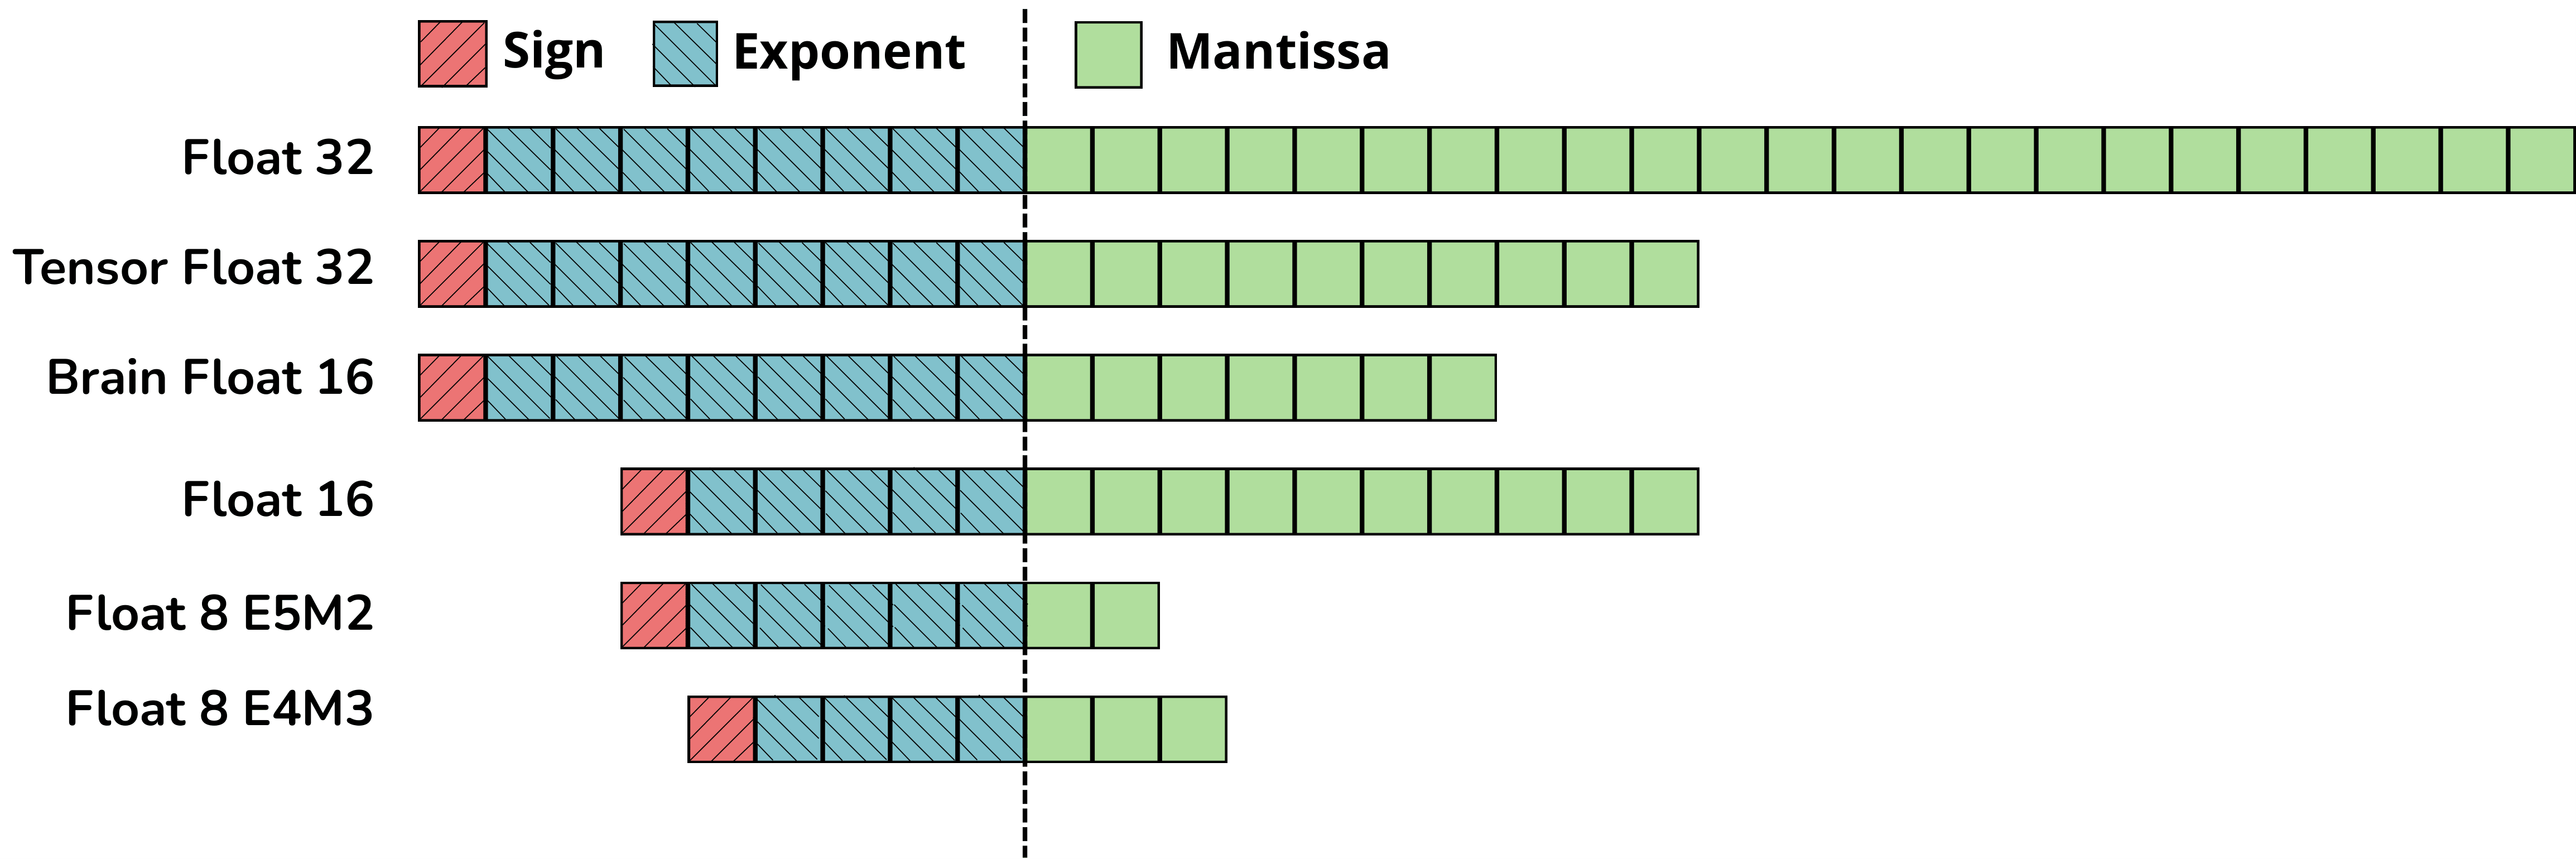
\includegraphics[width=\textwidth]{figs/Precision with hatch.pdf}
    \caption{Mixed Precision Floating-Point formats.}
    \tagpdfsetup{alttext={Mixed Precision Floating-Point formats.}}
    \label{fig:floating}
\end{figure}

Currently, two main types of FP8 quantization are used: W8A16 (8-bit weights and 16-bit activations) and W8A8 (8-bit weights and 8-bit activations). In particular, W8A8 typically employs the E4M3 format (4 exponent bits and 3 mantissa bits) for weights, and the E5M2 format (5 exponent bits and 2 mantissa bits) for activations. These two approaches target different hardware configurations. The former utilizes dedicated FP8 functional units to accelerate computation, while the latter is designed for hardware that only supports half-precision operations but still benefits from reduced memory usage.
Other quantization methods exist, but they fall outside the scope of this evaluation.

\subsection{Multi-GPU Inference}
\label{chap:background:sec:multigpu}

Growing model sizes and throughput requirements frequently exceed the memory and compute capacity of a single device, motivating multi-GPU strategies that distribute computation at the cost of increased communication. A variety of parallelism techniques have therefore been developed to balance memory capacity, communication overheads, and GPU utilisation.

\begin{figure}[h!]
    \centering
    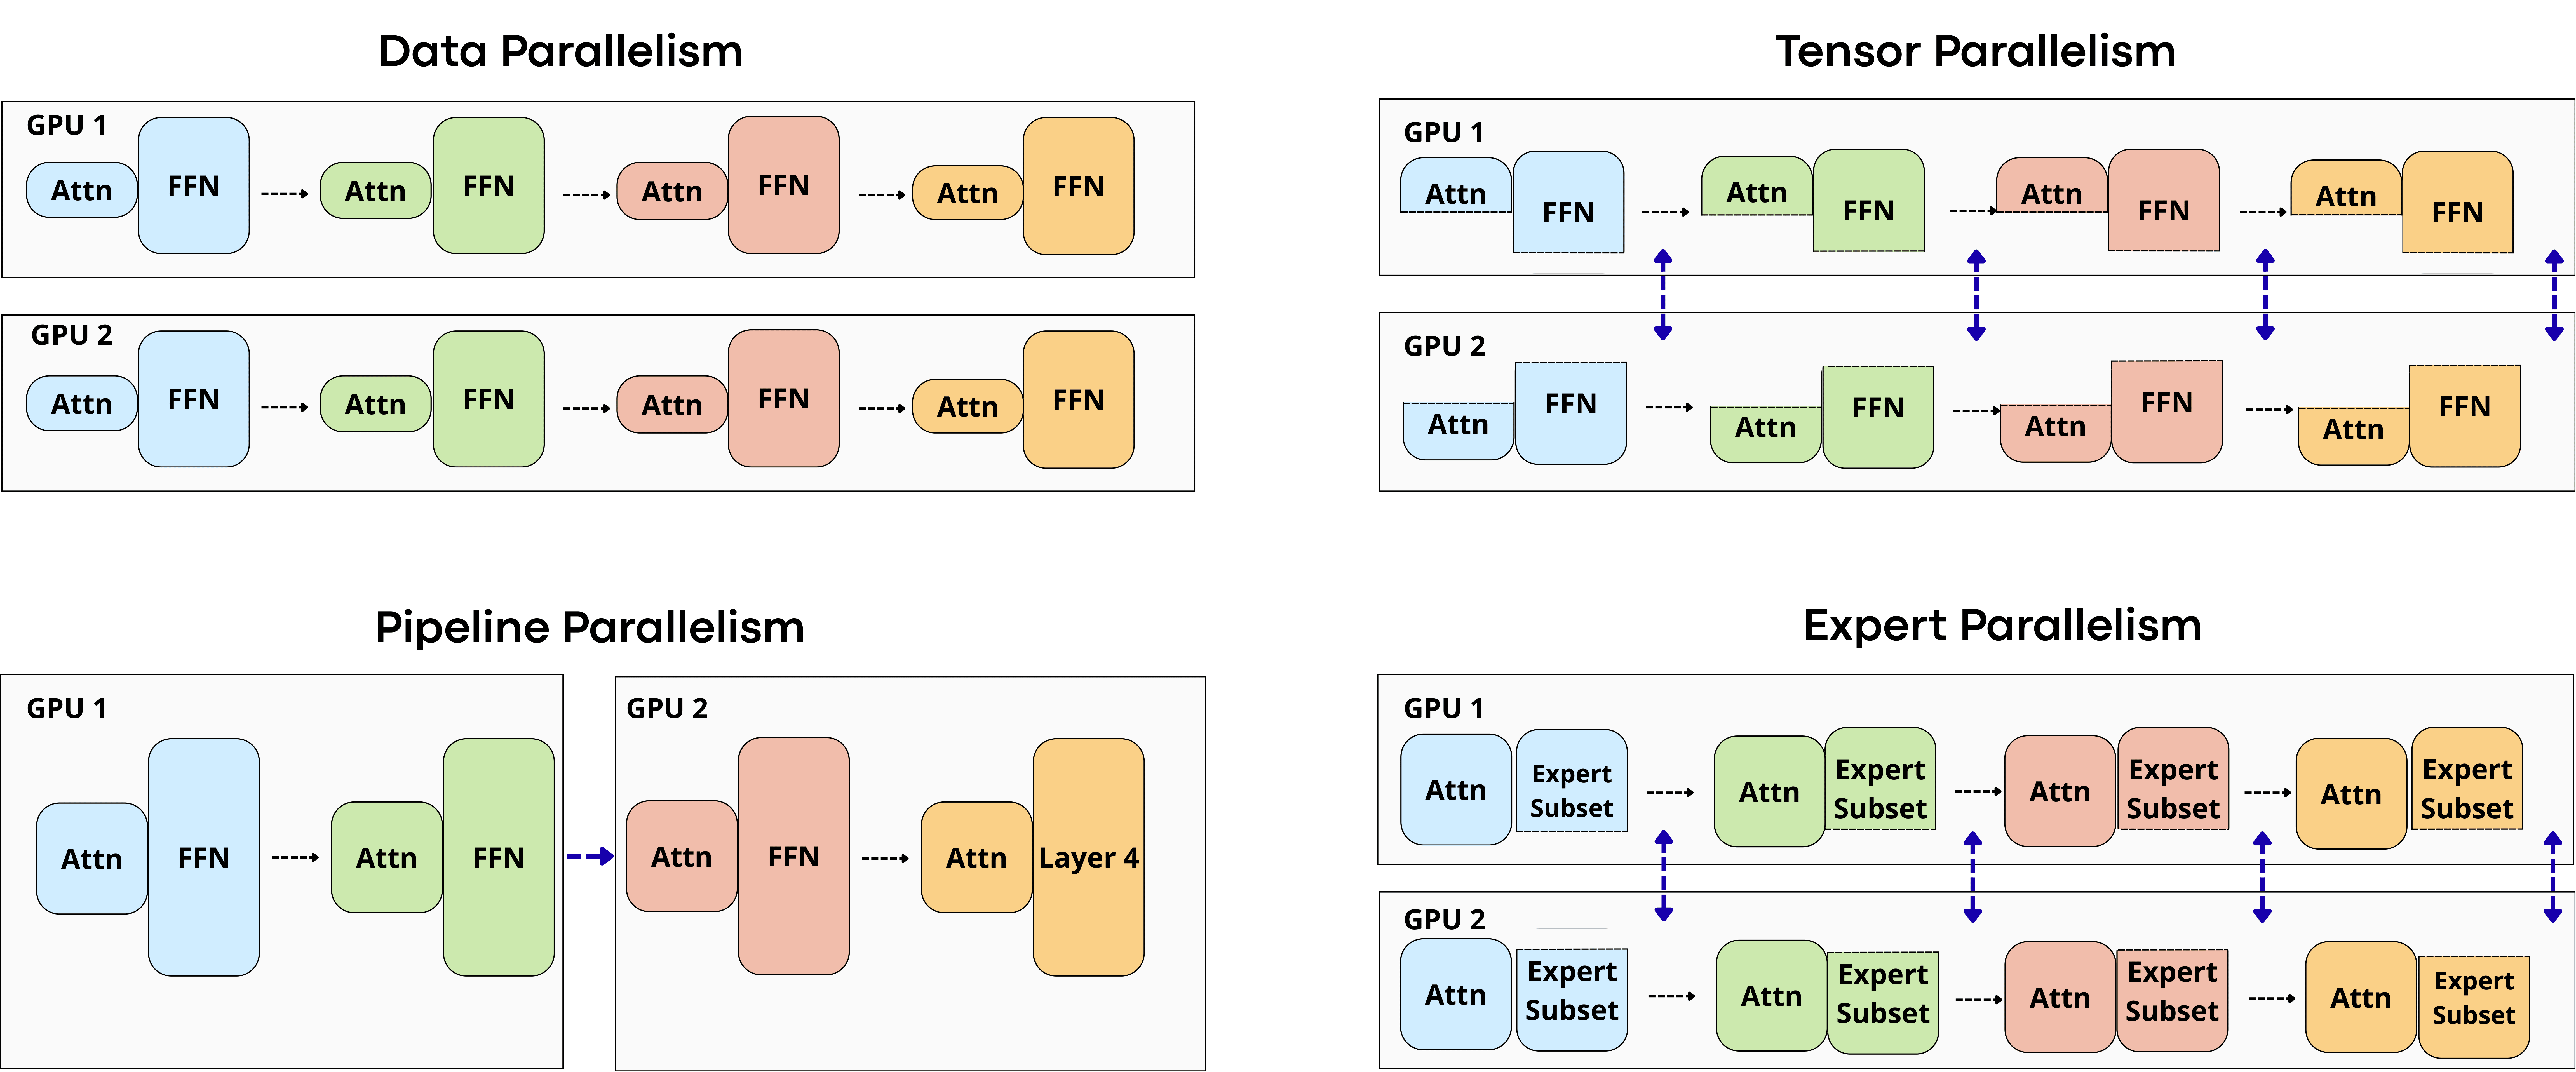
\includegraphics[width=0.95\textwidth]{figs/parallelism.pdf}
    \vspace{5mm}
    \caption{Comparison of multi-GPU techniques.}
    \tagpdfsetup{alttext={Comparison of multi-GPU techniques.}}
    \label{fig:parallel}
\end{figure}

\begin{itemize}
    \item \textbf{Data Parallelism (DP)} launches multiple independent model replicas on separate GPUs to increase serving throughput. Because each replica contains the full set of parameters, DP does not increase the effective memory available to a single model instance, but it scales well and requires no inter-GPU communication during inference.

    \item \textbf{Pipeline Parallelism (PP)} partitions the model’s layers across GPUs. Each device executes a contiguous block of layers and forwards intermediate activations to the next device. This expands the memory capacity accessible to a single model instance while introducing only moderate communication overhead.

    \item \textbf{Tensor Parallelism (TP)} shards parameters within each layer—such as attention heads and feed-forward weights—across multiple GPUs. This provides a finer-grained way to increase total available memory and keep all devices active, at the cost of frequent collective operations (e.g., all-gather).

    \item \textbf{Expert Parallelism (EP)} distributes the experts in Mixture-of-Experts layers across devices, allowing each GPU to store only a subset of expert parameters. Non-expert components—such as attention projections, layer norms, and routing modules—remain replicated on all devices. As a result, EP increases effective memory capacity primarily for expert-heavy layers while leaving the rest of the model duplicated.
\end{itemize}
\chapter{Background: Hardware Accelerators}
\label{chap:hardware}

LLM inference is a highly computational task dominated by large-scale matrix–matrix multiplications. This process poses three main challenges:
\begin{itemize}
    \item \textbf{Computation}: It requires executing a large number of floating-point operations.
    \item \textbf{Memory capacity}: It involves storing massive weight and activation matrices.
    \item \textbf{Memory bandwidth}: It demands frequent loading of large data volumes from memory.

\end{itemize}
For instance, performing a single forward pass of a 70-billion-parameter model in half precision (16-bit) entails approximately 140 BFLOPs of computation and 140 GB of memory reads.

To address these challenges, researchers have developed various parallel hardware accelerators that combine high memory bandwidth with large-scale parallel computing capabilities. Currently, Graphics Processing Units (GPUs) remain the dominant platform for LLM inference. However, Domain-Specific Architectures (DSAs) are emerging as promising alternatives, designed to provide greater efficiency for AI workloads \cite{chen2020survey, koilia2024hardware, silvano2025survey, kachris2025survey}.

This chapter provides a historical overview of the evolution of data center hardware accelerators used for AI inference, highlighting the key architectural trends shaping today’s computing landscape.

\section{Graphic Processing Units}
\label{chap:background:sec:gpu}

Graphics Processing Units (GPUs) are the most established class of accelerators for large-scale AI inference. They are designed around the \textbf{Single Instruction, Multiple Threads (SIMT) model}, which enables the parallel execution of thousands of lightweight threads. This parallelism makes GPUs highly efficient for the matrix and vector operations central to LLM inference. To support these operations, GPUs use a \textbf{multi-level memory hierarchy} that includes large off-chip DRAM for global storage and faster on-chip SRAM memories shared among thread blocks, ensuring high data throughput.

Modern General-Purpose GPUs (GPGPUs) emerged with NVIDIA’s Tesla architecture (2007) \cite{lindholm2008nvidia}, which transformed GPUs from fixed-function graphics devices into programmable, massively parallel processors. Tesla introduced uniform, fully programmable cores capable of dynamic workload balancing and non-graphics computations. Each GPU integrated 16 Streaming Multiprocessors (SMs), each containing 8 CUDA cores operating under the SIMT model. This architecture executed instructions in groups of 32 threads, known as warps, achieving SIMD-like efficiency while allowing limited control-flow divergence.

Tesla also established the standard GPU memory hierarchy still in use today—comprising per-thread \textbf{local memory}, per-SM \textbf{shared memory}, and \textbf{global DRAM}—along with L1 caches per SM and a unified L2 cache for improved data locality. Complementing this hardware innovation, NVIDIA introduced the \textbf{CUDA} programming model, a C/C++ extension that provides APIs for CPU–GPU coordination, memory management, and thread scheduling. CUDA laid the foundation for general-purpose GPU computing, enabling efficient deployment of parallel workloads such as deep learning inference.

This section presents the architecture of the most relevant data center–level GPUs developed by NVIDIA, AMD, and Intel, highlighting their evolution and design principles for AI inference workloads.

\subsection{NVIDIA GPUs}

Modern NVIDIA AI-oriented GPUs fall in the category of Tensor-Core GPUs. Their distinctive features are the presence of high-speed off-chip HBM memories, as opposed to standard DRAM, and the Tensor Cores, which accelerate matrix-matrix multiplications in mixed precision.
The NVIDIA P100 was the first to feature HBM memory, while the \textbf{NVIDIA Volta V100} \cite{choquette2018volta} first introduced Tensor Cores, representing a pivotal point in AI hardware.
In the remainder of this section, we provide a detailed discussion of the architectures of the NVIDIA V100, A100, and H100.

The \textbf{Nvidia Volta V100} is composed of six GPU Processing Clusters (GPCs) and features a total of 80 Streaming Multiprocessors (SMs). Each SM has four processing blocks, each featuring dedicated cores for single- and double-precision floating-point numbers and integer types. They also feature a Special Functional Unit (SFU) and two \textbf{Tensor Cores}: a dedicated functional unit that performs a matrix-matrix multiplication and accumulation.
Another major novelty is the unification of the L1 cache and the shared memory. According to the application's needs, the programmer can utilize up to 96 KB of the 128 KB L1 cache as shared memory, reserving the remaining space for caching.
The chip also offers 6MB of L2 cache, shared by all the GPCs, that acts as an intermediary between the SMs and the off-chip memory, consisting of 16 GB of HBM2 that operates at 0.90 TB/s.

The \textbf{NVIDIA Ampere A100} \cite{Choquette2021} represents a significant advancement over its predecessor, introducing numerous innovations and improvements.
It features 108 Streaming Multiprocessors, each divided into four processing blocks containing double-, single-, and integer-precision units, as well as third-generation Tensor Cores.
Unlike first-generation Tensor Cores, which are limited to FP16, the A100 cores support multiple data types (see \ref{tab:gpus}) and include fine-grained sparsity optimization, which doubles the throughput of sparse matrices. The \textbf{TF32} format is notable for combining the 8-bit exponent of FP32 with the 10-bit mantissa of FP16, offering a balance between precision and efficiency. The A100 also improves data delivery to the Tensor Cores by introducing asynchronous copy operations.
To support larger models, the size of memory is significantly increased: the L2 cache is increased to 40 MB, and the VRAM is either 40 or 80 GB of HBM2. There is also an improvement of $2.3\times$ in L2 cache throughput and $1.7\times$ in HBM throughput. Additionally, the A100 offers an in-hardware data compression feature that improves bandwidth by up to $4\times$.
The A100 also introduces two notable novelties: the third-generation NVLink and the Multi-Instance GPU (MIG) feature, which enables support for up to seven independent virtual GPUs on the same physical GPU.

The \textbf{NVIDIA Hopper H100} \cite{Choquette2023} represents an ulterior step forward with respect to the NVIDIA Ampere A100, featuring 132 redesigned Streaming Multiprocessors. Each multiprocessor comprises four processing blocks that integrate double-, single-precision, and integer units, as well as a fourth-generation Tensor Core.
The renewed Tensor Cores support improves throughput compared to the predecessor and adds support for 8-bit floating-point (\textbf{FP8}) precision (see \ref{fig:floating}).
The memory is improved by upgrading the off-chip DRAM to HBM3 and by increasing the sizes of the L1 and L2 caches.
To improve data locality, the Hopper architecture adds a new level in the CUDA hierarchy: the \textbf{thread block cluster}, which sits between the thread blocks and the grid and consists of up to 16 thread blocks. The cluster can benefit from improved data locality thanks to the new SM-to-SM communication network, which allows SMs to access the shared memory of other Streaming Multiprocessors and synchronize on barriers distributed across shared memory.
The Hopper Architecture also offers the fourth generation of NVLink and new types of barriers that facilitate asynchronous execution of threads and asynchronous data transfers.

Together with Hopper, NVIDIA also introduced \textbf{Grace}, a CPU featuring 72 Arm v9.0 cores explicitly designed to be paired with a GPU on a CPU-GPU System on a Chip (SoC). 
The \textbf{Grace-Hopper GH200} features a Grace CPU and a Hopper H100 GPU interconnected by a 900 GB/s cache coherent interconnection (NVLink-C2C). In total, the SoC has 96 GB of HMB memory and 512 GB of LPDDR5X DRAM. All the memory can be directly accessed by both processors, as they share the same system-wide page table.

\subsection{AMD GPUs}

In 2017, AMD introduced the Instinct MI series, derived from the Vega architecture and designed for scientific computing and AI workloads. In 2020, AMD separated its GPU lineup into RDNA for graphics and CDNA for data center computing, with CDNA architectures removing rendering features and adding dedicated matrix-multiply units similar to NVIDIA’s Tensor Cores. As noted by AMD researchers \cite{Loh2023}\cite{Smith2024}, CDNA designs are closely linked to the AMD EHP concepts developed under the U.S. Department of Energy’s Exascale Computing Program, representing early steps toward exascale-ready CPU–GPU systems.

The \textbf{AMD Instinct MI100} is the first CDNA GPU.
It features 120 Compute Units (CU) organized in four arrays. CUs feature both scalar and vector capabilities, thanks to dedicated register files, execution units, and cache for both scalar and vector operations. Vector execution units execute 64-wide wavefronts (similar to NVIDIA warps) over four cycles, thanks to a 16-wide SIMD vector pipeline that operates on both single- and double-precision data types.
The novelty of CDNA CUs lies in the introduction of Matrix Fused Multiply-Add (MFMA) units, which, similar to NVIDIA Tensor Cores, perform matrix-matrix multiplications.
The memory hierarchy of CDNA consists of the scalar and vector data caches of CUs, an 8 MB L2 cache shared by all CUs, and 32 GB of off-chip HMB2 memory that operates at 1.23 TB/s.
The MI100 is also the first card to feature AMD's Infinity Fabric technology, which enables inter-GPU communication similar to NVIDIA's NVLink.

\textbf{AMD CNDA 2:} The second generation of AMD CDNA cards represents an important step forward in AMD's GPU design.
The basic building block of CDNA 2 GPUs is called the Graphics Compute Die (GCD). Each GCD features four arrays of 28 compute units, totaling 112 (with 104 active in the MI210 and MI250, and 110 active in the MI250X). CDNA 2 introduces the concept of \textbf{multi-die GPUs}, significantly enhancing computational power. While the MI210 features a single GCD, the MI250 and MI250X are equipped with two GCDs, effectively doubling both the computational performance and memory capacity within a single board.
The Compute Units feature includes scalar, vector, and matrix cores. Vector cores operate on 64-wide wavefronts with 16-wide pipelines, supporting both single- and double-precision data types. Compared to its predecessor, the CDNA 2 Compute Units improve double-precision performance by a factor of two and support the new packed floating-point data type, enabling faster throughput for floating-point operations. Additionally, the matrix units undergo significant improvements, improving throughput and adding support for double-precision matrices.
Regarding memory, each GCD features 8 MB of L2 cache and 64 GB of HBM2e memory (1.6 TB/s).
A major innovation of CDNA 2 is the adoption of an innovative caching system that enables a unique memory addressing space for both the CPU and GPU, simulating an APU system where no CPU-GPU data transfers are necessary. 

\textbf{AMD CNDA 3:} The third generation of CDNA cards adopts an even more advanced approach to dense integration than CDNA 2, combining multiple dies within a single chip. This design realizes the 12-year-old AMD vision of a heterogeneous APU\cite{Smith2024}, incorporating both CPUs and GPUs on the same chip. The  DNA 3 family features two cards: the MI300X and the MI300A. The MI300X features eight accelerator complex dies (XCDs), similar to CDNA 2 GCDs, while the MI300A features six XCDs and three CPU complex dies (CCDs). 
The XCD features 40 CUs (38 active) and a set of shared resources, including the scheduler and four Asynchronous Compute Engines (ACE) that assign computing tasks to the Compute Units (CUs). The CUs also share 4 MB of L2 cache and have 32 KB of L1 cache each.
The biggest improvement compared to the previous generation is in the Matrix Cores, which offer improved performance compared to the previous generation and support new data types (Tensor Float and FP8).
Another important difference from the previous generation is the introduction of a new level of cache called Infinity cache, which sits between the off-chip memory and the on-chip L2 cache. The off-chip memory also underwent significant improvement, offering 128 GB of HMB3 memory (5.3 TB/s) on the MI300A and 192 GB on the MI300X. Similar to CDNA 2, CDNA 3 provides a unique memory addressing space shared by the CPU and the GPU, with the notable difference that in the MI300A APU, the memory is not only logically but also physically shared between the CPU and the GPU.

\subsection{Intel GPUs}

The Intel Xe GPU lineup, formerly known as Intel Ponte Vecchio \cite{gomes2022ponte}, comprises three models: the Intel Max 1100, Intel Max 1350, and Intel Max 1550. The latter powers the Aurora Supercomputer.

The \textbf{Intel Max 1550} is a multi-tile GPU featuring two Xe-stacks. Each Xe-stack contains four Xe-slices, providing a total of 64 Xe-cores, 64 ray-tracing units, and one media engine. Every Xe-core integrates eight vector engines (512-bit wide) and eight matrix engines (4096-bit wide). The vector engines support FP16, FP32, and FP64 data formats, while the matrix engines handle int8, FP16, and bfloat16 precisions.

In terms of memory, each Xe-core includes 512 KB of SRAM, which functions as shared memory or L1 cache. Each Xe-stack also incorporates 204 MB of shared L2 cache.

\ref{tab:gpus} summarizes all the architectural features of the modern AI GPUs discussed in this section.

\begin{table}[h!]
\centering
\footnotesize
\caption{Datacenter-level GPUs from Nvidia, AMD, and Intel.}
\label{tab:gpus}

\begin{tabularx}{\textwidth}{l l c c c c c c}
\toprule
\textbf{Vendor} & \textbf{Name} & \textbf{Year} & \textbf{Cores} & \textbf{TFLOPS} & \textbf{Cache} & \textbf{RAM} & \textbf{TDP} \\
\midrule

\textbf{NVIDIA}
& \textbf{V100}  & 2017 & 80 SM  & \makecell[l]{TF32: 125} 
& \makecell[l]{L1: 128 KB \\ L2: 16 MB} 
& \makecell[l]{HBM2: 32 GB \\ 0.90 TB/s} 
& 400 W \\

\textbf{NVIDIA}
& \textbf{A100}  & 2020 & 108 SM 
& \makecell[l]{TF32: 156 \\ FP16: 312} 
& \makecell[l]{L1: 164 KB \\ L2: 40 MB} 
& \makecell[l]{HBM2e: 80 GB \\ 2.03 TB/s} 
& 400 W \\

\textbf{NVIDIA}
& \textbf{H100}  & 2022 & 132 SM 
& \makecell[l]{TF32: 989 \\ FP16: 1979 \\ FP8: 3958} 
& \makecell[l]{L1: 256 KB \\ L2: 50 MB} 
& \makecell[l]{HBM3: 80 GB \\ 3.35 TB/s} 
& 700 W \\

\textbf{NVIDIA}
& \textbf{GH200} & 2023 & 132 SM 
& \makecell[l]{TF32: 989 \\ FP16: 1979 \\ FP8: 3958} 
& \makecell[l]{L1: 256 KB \\ L2: 50 MB} 
& \makecell[l]{HBM3: 96 GB \\ 3.9 TB/s} 
& 450 W \\

\midrule

\textbf{AMD}
& \textbf{MI100}  & 2020 & 120 CU 
& \makecell[l]{FP32: 23 \\ FP16: 185} 
& \makecell[l]{L1: 16 KB \\ L2: 8 MB} 
& \makecell[l]{HBM2e: 32 GB \\ 1.2 TB/s} 
& 560 W \\

\textbf{AMD}
& \textbf{MI250}  & 2021 & 220 CU 
& \makecell[l]{FP32: 90 \\ FP16: 362} 
& \makecell[l]{L1: 16 KB \\ L2: 16 MB} 
& \makecell[l]{HBM2e: 128 GB \\ 3.2 TB/s} 
& 500 W \\

\textbf{AMD}
& \textbf{MI300X} & 2023 & 304 CU 
& \makecell[l]{TF32: 654 \\ FP16: 1307 \\ FP8: 2615} 
& \makecell[l]{L1: 32 KB \\ L2: 4 MB \\ L3: 256 MB} 
& \makecell[l]{HBM3: 192 GB \\ 5.3 TB/s} 
& 750 W \\

\textbf{AMD}
& \textbf{MI300A} & 2023 & 228 CU 
& \makecell[l]{TF32: 490 \\ FP16: 980 \\ FP8: 1961} 
& \makecell[l]{L1: 32 KB \\ L2: 4 MB \\ L3: 256 MB} 
& \makecell[l]{HBM3: 128 GB \\ 5.3 TB/s} 
& 760 W \\

\midrule

\textbf{Intel}
& \textbf{MAX 1550} & 2023 & 128 Xe 
& \makecell[l]{FP16: 832} 
& \makecell[l]{L1: 64 KB \\ L2: 408 MB} 
& \makecell[l]{HBM2e: 128 GB \\ 3.28 TB/s} 
& 600 W \\

\bottomrule
\end{tabularx}
\end{table}

\subsection{GPU limitations: the memory wall}

As discussed earlier, Graphics Processing Units (GPUs) are the most widespread type of hardware accelerator for LLM inference. Their success stems from their ability to perform massive numbers of floating-point operations in parallel, which is essential for deep neural network (DNN) training and inference. By scaling out the number of cores, GPUs have sustained performance growth despite the slowdown in transistor miniaturization and the onset of dark silicon.

However, GPUs often fail to reach their theoretical peak throughput during large language model (LLM) inference because these workloads are typically \textit{memory-bound}. As shown in Table~\ref{tab:gpus}, GPU compute throughput (in FLOPS) exceeds memory bandwidth by up to two orders of magnitude, meaning that data transfer between memory and compute units dominates latency and limits overall performance.

Gholami et al.~\cite{gholami2024ai} highlight that this imbalance is widening over time. While floating-point performance has increased by a factor of three every two years, memory bandwidth has increased by only about 1.6 times per year.
This growing disparity between computation and data movement is known as the \textbf{memory wall}~\cite{gholami2024ai}.

To mitigate this limitation, researchers have developed \textit{Domain-Specific Architectures (DSAs)} designed to minimize data transfer during DNN inference and training~\cite{Hooker2021, Dean2018}. The first prominent example was Google’s \textbf{Tensor Processing Unit (TPU)}~\cite{Jouppi2017}, which demonstrated how customized architectures can achieve substantial gains in both speed and energy efficiency.

\newpage
\section{AI Accelerators - TPUs}\label{chap:background:sec:tpu}

This section describes the design \textbf{Tensor Processing Units (TPU)} and other architectures that share common features. \ref{tab:tpus} summarises the main features of the architectures discussed in this section, namely Google TPUs, Habana Lab TPCs, and Groq LPus.

\begin{table}[h!]
\centering
\footnotesize
\caption{Tensor-Core based accelerators from Google, Habana Labs, and Groq.}
\label{tab:tpus}

\begin{tabularx}{\textwidth}{l l c c c c c c}
\toprule
\textbf{Vendor} & \textbf{Name} & \textbf{Year} & \textbf{Cores} & \textbf{Data Types} & \textbf{On-chip} & \textbf{Off-chip} & \textbf{TDP} \\
\midrule

\textbf{Google}
& \textbf{TPU v1}  & 2015 & \makecell[l]{1 core \\ 1 MXU/core} & int8 
& 28 MB & DDR3: 8 GB & 75 W \\

\textbf{Google}
& \textbf{TPU v2}  & 2017 & \makecell[l]{2 cores \\ 1 MXU/core} & BF16 
& 32 MB & HBM: 16 GB & 280 W \\

\textbf{Google}
& \textbf{TPU v3}  & 2018 & \makecell[l]{2 cores \\ 2 MXU/core} & BF16 
& 32 MB & HBM: 32 GB & 450 W \\

\textbf{Google}
& \textbf{TPU v4}  & 2021 & \makecell[l]{2 cores \\ 4 MXU/core} & BF16, int8 
& 32 MB & HBM: 32 GB & N/A \\

\textbf{Google}
& \textbf{TPU v4i} & 2021 & \makecell[l]{1 core \\ 4 MXU/core} & BF16, int8 
& 144 MB & HBM: 32 GB & 175 W \\

\textbf{Google}
& \textbf{TPU v5e} & 2023 & \makecell[l]{1 core \\ 4 MXU/core} & BF16, int8 
& 112 MB & HBM: 16 GB & N/A \\

\textbf{Google}
& \textbf{TPU v5p} & 2023 & \makecell[l]{2 cores \\ 4 MXU/core} & BF16, int8 
& 48 MB & HBM: 95 GB & N/A \\

\textbf{Google}
& \textbf{TPU v6e} & 2024 & \makecell[l]{1 core \\ 4 MXU/core} & BF16, int8 
& N/A & HBM: 32 GB & N/A \\

\textbf{Google}
& \textbf{TPU v7p} & 2025 & N/A & BF16, FP8 
& N/A & HBM: 192 GB & N/A \\

\midrule

\textbf{Habana}
& \textbf{Goya}    & 2018 & \makecell[l]{8 TPC \\ 1 MME} 
& int8 
& 28 MB & DDR4: 16 GB & N/A \\

\textbf{Habana}
& \textbf{Gaudi}   & 2019 & \makecell[l]{8 TPC \\ 1 MME} 
& FP32, int8 
& 24 MB & HBM2: 32 GB & N/A \\

\textbf{Habana}
& \textbf{Gaudi 2} & 2022 & \makecell[l]{24 TPC \\ 2 MME} 
& \makecell[l]{FP32, BF16 \\ FP16, FP8} 
& 48 MB & HBM: 96 GB & 600 W \\

\textbf{Habana}
& \textbf{Gaudi 3} & 2024 & \makecell[l]{64 TPC \\ 8 MME} 
& \makecell[l]{FP32, TF32 \\ FP16, BF16, FP8} 
& 96 MB & HBM: 128 GB & 900 W \\

\midrule

\textbf{Groq}
& \textbf{GroqCard} & 2019 & 320 lanes 
& \makecell[l]{int8, int16 \\ FP16} 
& 230 MB & -- & 275 W \\

\bottomrule
\end{tabularx}
\end{table}

\subsection{Google TPU}
\label{chap:background:sec:tpu}

In 2013, Google began developing the \textbf{Tensor Processing Unit (TPU)}, the first domain-specific accelerator for neural network inference. At that time, CPUs were used for inference and GPUs for training, but this approach was both costly and energy-intensive. To address this, Google designed a single-core, domain-specific processor centred on a \textbf{Matrix Multiply Unit (MXU)}, a systolic array specialised for dense matrix multiplications. This architecture minimized energy-hungry memory accesses and control operations through spatial computation~\cite{jouppi2018motivation}, achieving order-of-magnitude improvements in efficiency and marking the start of domain-specific architectures for AI.

Several TPU generations (v1–v7) have since been released, summarised in Table~\ref{tab:tpus}. The main architectural features of the first four generations—those publicly documented—are outlined below.

\textbf{TPU v1}~\cite{Jouppi2017} was a PCIe-attached co-processor optimized for inference. Its core component, the 256×256 \textbf{MXU}, consisted of 65,536 int8 multipliers operating in a systolic array that streamed data directly between adjacent cells. Each cycle produced 256 partial sums, accumulated in on-chip registers. The chip included 24~MB of on-chip SRAM (the Unified Buffer) for activations and 8~GB of off-chip DDR3 DRAM for weights. A Very Long Instruction Word (VLIW) control unit allowed the compiler to statically schedule parallel operations, simplifying control logic while maintaining high utilisation.

\textbf{TPU v2 and v3}~\cite{Norrie2021} extended the design for training workloads, introducing \textbf{bfloat16} arithmetic to replace int8 quantisation, providing a balance between precision and hardware cost. Each core integrated a scalar unit, vector unit, and MXU arranged in a push–pop pipeline, where the MXU acted as a co-processor for the vector unit. Memory organisation was restructured into a unified \textbf{Vector Memory} scratchpad, while off-chip DDR was replaced by 16~GB of \textbf{HBM}, boosting bandwidth by over 20×. TPU v2 adopted a dual-core layout with a 2D torus interconnect for large-scale scaling. TPU v3 doubled the MXUs per core, increased clock speed, expanded HBM capacity, and improved inter-chip bandwidth, enabling significantly higher throughput for large models.

\textbf{TPU v4i}~\cite{Jouppi2021}, introduced in 2021, was designed as an inference-oriented counterpart to the training-focused TPU v4. It retained the systolic array architecture but incorporated four MXUs per core for increased parallelism. The memory hierarchy added a new 128~MB \textbf{Common Memory (CMEM)} layer between on-chip vector memory and off-chip HBM, reducing data transfer overhead. TPU v4i supported both int8 and bfloat16 data types, reflecting the industry trend toward higher precision inference. Like previous versions, it used HBM to sustain high bandwidth and employed dedicated SRAM regions for scalar values and instructions.

\textbf{TPU v5–v7} continue this evolution, though details are mostly undisclosed. The fifth generation includes two variants: \textbf{TPU v5p} (performance-optimised) and \textbf{TPU v5e} (cost-efficient), both with four MXUs per core and support for int8 and bfloat16. The sixth-generation \textbf{TPU v6e (Trillium)} doubles memory capacity and introduces 256×256 MXUs per core, while the forthcoming \textbf{TPU v7p (Ironwood)} further increases memory (192~GB) and adds support for 8-bit floating-point formats, signalling a shift toward finer precision–efficiency trade-offs in inference hardware.

\subsection{Habana Labs TPC}
\label{chap:background:sec:habana}

Founded in 2016 and acquired by Intel in 2019, \textbf{Habana Labs} introduced the \textbf{Tensor Processing Core (TPC)} architecture in 2018, a family of domain-specific AI accelerators for inference and training. Similar to Google’s TPUs, Habana’s design centres on specialised matrix multiplication engines integrated with programmable compute cores. The company’s main lineup includes the inference accelerators \textbf{Goya} (2018) and \textbf{Greco} (2022), and the training accelerators \textbf{Gaudi} (2019), \textbf{Gaudi2} (2022), and \textbf{Gaudi3} (2024).

\textbf{Habana Goya}~\cite{Gwennap2019} was the first inference processor, featuring an HL-1000 chip with eight \textbf{TPCs}, one \textbf{Matrix Multiplication Engine (MME)}, and a hierarchical memory system. Each TPC is a VLIW SIMD processor supporting integer and floating-point operations (8–32 bits). The MME is a 256×256 systolic array for int8 matrix multiplication shared across all TPCs. Goya uses 16 GB DDR4 memory and on-chip SRAM, optimised for low-latency, energy-efficient inference.

\textbf{Habana Gaudi}~\cite{Gwennap2019} adapted Goya for training, adding floating-point GEMM support, 32~GB of high-bandwidth \textbf{HBM2} memory, and ten 100~Gb/s Ethernet links for direct chip-to-chip communication, enabling distributed training without host coordination.

\textbf{Habana Gaudi2}~\cite{gaudi2} significantly scaled the architecture, tripling TPCs (8→24) and HBM capacity (6×16~GB HBM2E). It also expanded interconnect bandwidth with 24 100-Gb/s Ethernet ports and introduced mixed-precision support—\textbf{FP32}, \textbf{bfloat16}, \textbf{FP16}, and \textbf{FP8} — across both TPCs and GEMM units. Dedicated decoding engines were added for handling compressed image and video data.

\textbf{Habana Gaudi3}~\cite{Kaplan2024} further scaled the design to four clusters, each with 16 TPCs and two MMEs, totalling 96 TPCs and eight GEMM units. On-chip memory was expanded from 48~MB SRAM to a 96~MB L2 cache, while external memory grew to eight 16~GB HBM2E stacks, offering higher parallelism, bandwidth, and scalability for large AI workloads.

\subsection{Groq LPU}

The Groq Language Processing Unit (LPU) \cite{Gwennap, Abts2022} is a dataflow accelerator introduced in 2019 by Groq.
The LPU is built as a systolic array of heterogeneous functional units where data flows horizontally through lanes and instructions vertically across them. Sixteen lanes form a superlane, and the LPU contains 20 active superlanes plus one redundant lane. Each superlane processes streaming data through a Vector Unit, Memory Unit, Switch Unit, and Matrix Unit arranged symmetrically into eastward and westward hemispheres. The Vector Unit has 16 ALUs supporting integer–floating-point conversions and activation functions. The Memory Unit provides 44 slices of 128 kB SRAM (5.5 MB total) with up to two reads and writes per cycle for instructions and activations. The Switch Unit handles tensor reshaping, while the Matrix Unit includes 320 MACs per lane optimised for int8 but also supporting int16 and FP16. So, in total, each superlane features 20 $16\times 16$ matrix-matrix multiplication units.

Groq LPU design resembles Google's TPU as it includes vector and matrix-matrix multiplication functional units optimised for integer operations. On the other hand, the way instructions are pipelined through the lanes is drastically different from Google's design. Another key difference is the absence of DRAM memory and caches, which allows the LPU to achieve full determinism, allowing its compiler to statically schedule every operation with cycle-accurate predictability.

\section{AI Accelerators - Dataflow}\label{chap:background:sec:dflow}

This section describes the second class of Domain-Specific Accelerators for LLM inference, which consists of \textbf{dataflow accelerators}. \ref{tab:dflow} summarizes the main features of the architectures discussed in this section, namely SambaNova RDAs, Cerebras WSE, and GraphCore IPUs.

\subsection{SambaNova RDA}
\label{chap:background:sec:sambanova}

Founded in 2017, \textbf{SambaNova Systems} develops dataflow accelerators for DNN training and inference, inspired by the \textbf{Plasticine} prototype architecture~\cite{Prabhakar2017}.

\textbf{Plasticine} is a coarse-grained reconfigurable architecture (CGRA) that exploits spatial parallelism for compute patterns such as map and reduce. Unlike bit-level FPGAs, CGRAs use word-level processing elements (ALUs, DSPs) connected through structured interconnects, achieving higher density and clock speeds. Plasticine consists of \textbf{Pattern Compute Units (PCUs)} and \textbf{Pattern Memory Units (PMUs)} arranged in a grid, managed by hierarchical controllers that coordinate pipelined and streaming execution. Address Generators and Coalescing Units handle off-chip memory, optimizing access patterns and reducing traffic.

Building on this concept, SambaNova’s \textbf{Reconfigurable Dataflow Architecture} \cite{sambanova} combines tiled PCUs and PMUs linked by a high-bandwidth switch fabric, with AGUs and CUs managing external memory. Its software stack, \textbf{SambaFlow}, integrates with PyTorch and TensorFlow, automatically mapping models to hardware. A Dataflow Graph Analyzer identifies dependencies, while the compiler optimizes execution through parallelization and pipelining. RDA also supports concurrent workloads, allowing simultaneous preprocessing, training, and inference tasks.

The first generation, the \textbf{Cardinal SN10-8R}, featured eight RDUs, each with 640 PCUs and PMUs, and up to 12~TB of configurable DRAM. Its successor, \textbf{Cardinal SN30-8R}, increased compute density to 1,284 PCUs and PMUs per RDU, with 640~MB on-chip memory and 1~TB of DRAM per device. The 2024 \textbf{SN40L-16}~\cite{Prabhakar2024}, optimized for LLM inference, integrates 16 RDUs with 1,040 PCUs and PMUs each, 520~MB of SRAM, and hybrid memory combining 64~GB HBM with 768~GB DDR—significantly boosting bandwidth for compute-bound workloads.


\subsection{Cerebras WSE}
\label{chap:background:sec:cerebras}

Founded in 2015, \textbf{Cerebras Systems} develops large-scale AI accelerators for DNN training and inference. The company has released three systems: the \textbf{CS-1} (2019) with \textbf{WSE-1}, the \textbf{CS-2} (2021) with \textbf{WSE-2}, and the \textbf{CS-3} (2024) featuring \textbf{WSE-3}.

The \textbf{Wafer-Scale Engine (WSE)} is the first processor built on a full 300~mm silicon wafer (462.25~cm$^2$), hosting 400{,}000 cores in WSE-1, 850{,}000 in WSE-2, and 900{,}000 in WSE-3. Each core is a general-purpose compute element supporting arithmetic, logic, and tensor operations through hardware state machines and \textbf{Data Structure Registers (DSRs)} that manage tensor metadata. The 64-bit datapath includes four fused FPMAC units operating on FP16 and bfloat16 data for high tensor throughput.

The WSE adopts a fully distributed memory architecture to maximize locality and bandwidth. Each core integrates 48~KB of SRAM, yielding 44~GB of total on-chip memory in WSE-3. Cores communicate through a 2D mesh of routers, allowing weights and activations to stream efficiently across the wafer and to external \textbf{MemoryX} units, removing the need for shared DRAM or intermediate buffers.

Computation follows a dataflow execution model where operations are triggered by data arrival rather than instruction sequencing. This enables fine-grained sparsity filtering and high energy efficiency. Each core supports dynamic scheduling with up to eight concurrent micro-threads, selecting ready operations based on data availability and priority to improve utilization and reduce latency.


\subsection{Graphcore IPU}
The \textbf{Intelligent Processing Unit (IPU)} by Graphcore is a dataflow-based accelerator designed for AI workloads. Two generations exist: the \textbf{Colossus MK1} (2017) with GC2 IPUs and the \textbf{Colossus MK2} (2020) with GC200 IPUs.

The IPU implements a true \textbf{MIMD} architecture following the \textbf{Bulk Synchronous Parallel (BSP)} model~\cite{Jia2019}, which structures computation into three stages: local execution on private memory, inter-tile communication, and global synchronization. Computation occurs on independent \textbf{tiles}, each with its own processor, local SRAM, and an \textbf{Accumulating Matrix Product (AMP)} unit optimized for matrix multiplications and convolutions. Tiles support up to six threads via SMT, with 1,216 cores (7,296 threads) in the first generation and 1,472 cores (8,832 threads) in the second. Each AMP unit performs up to 16~FP32 or 64~FP16 operations per cycle.

Tiles operate exclusively on local memory—256~KB in the GC2 and 624~KB in the GC200—eliminating caches and shared DRAM while ensuring deterministic performance. Inter-tile communication is handled by the on-chip \textbf{IPU Exchange} and off-chip \textbf{IPU Links}, enabling large-scale, multi-IPU systems.

Programming is performed using the \textbf{Poplar SDK}, where models are represented as computation graphs. The compiler maps graph vertices to threads and edges to communication paths, automatically managing the compute, communication, and synchronization phases under the BSP model.

\begin{table}[h!]
\centering
\footnotesize
\caption{Datacenter-level dataflow AI accelerators from SambaNova, Cerebras, and Graphcore.}
\label{tab:dflow}

\begin{tabularx}{\textwidth}{l l c c c c c c}
\toprule
\textbf{Vendor} & \textbf{Name} & \textbf{Year} & \textbf{Cores} & 
\textbf{TFLOPS} & \textbf{On-chip} & \textbf{Off-chip} & \textbf{TDP} \\
\midrule

\textbf{Graphcore}
& GC2   & 2017 & 1,216 & FP16: 125 
& 300 MB 
& -- 
& 150 W \\

\textbf{Graphcore}
& GC200 & 2020 & 1,472 & FP16: 250 
& 900 MB 
& -- 
& 300 W \\

\midrule

\textbf{SambaNova}
& SN10  & 2021 & 640 
& BF16: N/A 
& 300 MB 
& DRAM: 1.5 TB 
& N/A \\

\textbf{SambaNova}
& SN30  & 2022 & 1,284 
& BF16: 660 
& 640 MB 
& DRAM: 1 TB 
& N/A \\

\textbf{SambaNova}
& SN40L & 2023 & 1,040 
& BF16: 638 
& 520 MB 
& \makecell[l]{HBM: 64 GB \\ DRAM: 768 GB} 
& 900 W \\

\midrule

\textbf{Cerebras}
& CS2 (WSE2) & 2021 & 850K 
& BF16: N/A 
& 41 GB 
& MemoryX 
& 23 kW \\

\textbf{Cerebras}
& CS3 (WSE3) & 2024 & 900K 
& BF16: 125K 
& 44 GB 
& MemoryX 
& 23 kW \\

\bottomrule
\end{tabularx}
\end{table}
\chapter{Methodology}
\label{chap:methods}

With this thesis, we aim to measure and compare the LLM inference performance and energy efficiency of a diverse set of accelerated servers across multiple deployment scenarios. However, the heterogeneity of models, hardware, and software stacks, as well as the numerous interacting factors that influence performance, makes this task non-trivial. To structure our analysis, we begin by identifying the principal factors that impact LLM inference performance, focusing on four key elements:

\begin{itemize}
\item \textbf{Sequence length}: the number of input and output tokens generated. We ensure consistency by using the same inference dataset (Section \ref{chap:methods:sec:dataset}) for all experiments.
\item \textbf{Model architecture}: the characteristics of the LLM being served. We address the heterogeneity of LLM models by evaluating a diverse set of popular open-source models and examining their characteristics in relation to performance. In particular, we analyze:
\begin{itemize}
\item \textbf{Model Size}: the total number of model parameters;
\item \textbf{Sparsity}: the proportion of parameters that are sparsely activated, in the case of Mixture-of-Experts (MoE) models.
\item \textbf{Quantization}: the numerical format used for model weights and activations. Wherever supported, we compare 16-bit precision with 8-bit precision.
\end{itemize}
\item \textbf{Parallelism}: The number of sequences processed in parallel (\textbf{batch size}) and the number of devices used for inference greatly impact performance, depending on the parallel serving strategy chosen (\textbf{Data, Pipeline, Tensor or Expert Parallelism}).
\item \textbf{Inference Engine}: the software stack influences performance. We maintain consistency by using the same inference engine (vLLM \cite{kwon2023efficient}) across all the GPU servers. Dataflow accelerators, on the other hand, require an architecture-specific engine.
\end{itemize}

\section{LLM Inference Performance}
\label{chap:methods:sec:model}

In Section \ref{chap:background:sec:llms}, we introduced the typical decoder-only transformer architecture, which consists of a stack of layers that includes a self-attention block and a feed-forward network. While Section \ref{chap:background:sec:serving} discusses how these models are used for generating text outputs. In this section, we provide a detailed description of LLM inference, discussing how the four factors identified earlier affect the computational and memory workload.
This analysis enables us to critically analyze the results presented in Chapter \ref{chap:results}, understanding the distance between ideal and practical performance trends.

As discussed in Section \ref{chap:background:sec:serving}, an inference task requires processing the entire prompt during the prefill phase. Then, in the decode phase, a new token is generated per forward pass.
This meas that the total latency of the inference job can be identified as $\Delta t = \Delta t_{FP} \times(FP_{IN} + FP_{OUT})$, where $\Delta t_{FP}$ is the latency of the forward pass, $FP_{IN}$ is the number of forward passes needed for the prefill phase (typically 1), and $FP_{OUT}$ corresponds to the number of output tokens.

$\Delta t_{FP}$ depends on the specific software implementation and hardware accelerator that are being employed. But, in general, we can decompose it in two parts: $\Delta t_{FP} = \Delta t_{C} + \Delta t_{mem}$, where $\Delta t_{C}$ is related to the computation, and $\Delta t_{mem}$ is related to memory accesses.
With an accelerator with a throughput of $TP\  \text{OPs}/s$ and has a memory bandwidth of $BW\ \text{bytes}/s$, $\Delta t_{C} = C_{\text{forward}}/TP$ and $\Delta t_{C} = Mem/BW$, where $C_{\text{forward}}$ and $Mem$ are the number of operations and the amount of memory to access at each forward pass. 

By applying the formula proposed by Kaplan et al.~\cite{kaplan2020scaling}, we can estimate the forward-pass computational cost \( C_{\text{forward}} \) in terms of the language model architecture and the context length. Specifically, we characterize a model by its total parameter count \( N \), the number of layers \( n_\text{layer} \), the dimensionality of the attention layer output \( n_\text{model} \), and the number of attention head groups $ n_\text{groups}$.

For a model with size \( N \), the computational cost per forward pass can be approximated as
\[
C_{\text{forward}} \approx 2N + 2n_\text{layer} n_{\text{ctx}} d_{\text{attn}}.
\]

The first term refers to the context-independent FLOPs, which are related to the matrix-matrix multiplications associated with the $W^Q$, $W^K$, and $W^V$ projection matrices, as well as the feed-forward block. The second term, however, is context-dependent, as it scales linearly with the context length.
Kaplan et al.~\cite{kaplan2020scaling} argue that the context-independent component of the computation dominates the overall cost, enabling a simplification of the forward-pass complexity to $C_{\text{forward}} \approx 2N$, where the number of FLOPs scales linearly with the model size $N$.

To evaluate the validity of this hypothesis, we explicitly compute the FLOPs associated with both the context-dependent and context-independent components across five open-source models of varying sizes, selected from those used in our experimental evaluation. Table~\ref{tab:context_architecture} illustrates the relative contribution of these two components for different context lengths and increasing model scales. We observe that smaller models exhibit a larger relative impact from context-dependent operations. Nevertheless, for moderate context lengths (fewer than $10{,}000$ tokens), more than $85\%$ of the total computational cost consistently arises from the context-independent component across all models. This empirical evidence supports the robustness of the linear scaling trend for inputs of this size.

\begin{table}[h]
\centering
\caption{Percentage of context-independent FLOPs over total for different context lengths.}
\label{tab:context_architecture}
\begin{tabular}{lccccccc}
\toprule
\textbf{Model} & \textbf{Params} & \textbf{Layers} & \textbf{Hidden} &
\textbf{100} & \textbf{1,000} & \textbf{10,000} & \textbf{100,000} \\
\midrule
\textbf{Llama 3.1 8B}  & 8B      & 32 & 4096 & 99.8\% & 98.4\% & 85.9\% & 37.9\% \\
\textbf{Qwen3 14B}     & 14.8B   & 40 & 6144 & 99.9\% & 98.8\% & 89.5\% & 46.1\% \\
\textbf{Qwen3 32B}     & 32B     & 64 & 8192 & 99.9\% & 99.2\% & 92.4\% & 55.0\% \\
\textbf{Nemotron 49B}  & 49B     & 80 & 8192 & 99.9\% & 99.3\% & 93.7\% & 59.9\% \\
\textbf{Llama 3.3 70B} & 70B     & 80 & 8192 &100.0\% & 99.5\% & 95.5\% & 68.1\% \\
\bottomrule
\end{tabular}
\end{table}

Introducing parallelism across multiple sequences complicates the analysis: with a batch size $b$, each sequence requires $C_{\text{forward}}$ operations. If we neglect the context-dependent portion of the computation that differs across sequences, the total compute latency scales linearly with batch size,
\[
\Delta t_{C}(b) = b \times \Delta t_{C}(1),
\]
implying that the number of FLOPs per token remains constant for different values of $b$.
Memory accesses, instead, display a different behavior. The amount of memory (\( \text{Mem} \)) that is read at each forward pass consists of two parts: a context-independent component (the model’s weights) and a context-dependent component (the KV cache).  
For a sequence of length $n_{\text{ctx}}$ and a batch size $b$ the total amount of memory to read is
\[
Mem = NP_W + 2bn_\text{layer} n_{\text{ctx}} \frac{ d_{\text{model}} }{n_{\text{groups}}} P_A
\]
where $P_W$ is the number of bytes per weight, and $P_A$ is the number of bytes per value in the KV cache.
It is essential to note that, unlike computation, the amount of memory allocated per token is not constant with respect to the batch size, as access to the model weights is shared among all the sequences in the batch.

Using 1024 tokens as an example, we observe that for small batch sizes the contribution of the KV cache to the total memory footprint is negligible ($0.1\%$–$0.2\%$ across model sizes for $b=1$). However, as the batch size increases, the KV cache occupies a growing fraction of memory, particularly for smaller models, reaching $7.1\%$–$21.2\%$ at a batch size of $128$.

Once the number of operations and the memory footprint are identified, we have all the elements to compute the latency $\Delta t_{FP}$ under an idealized model:
\[
\Delta t_{FP} = \Delta t_{C} + \Delta t_{mem} = \frac{(2N + 2n_\text{layer} n_{\text{ctx}} d_{\text{attn}})b}{TP} + \frac{NP_W + 2bn_\text{layer} n_{\text{ctx}} \frac{ d_{\text{model}}}{n_{\text{groups}}} P_A}{BW} \approx \frac{2N}{TP} + \frac{NP_W}{BW}
\]
Where the approximation holds for $N >> b n_{\text{ctx}} d_{\text{model}}n_\text{layer}$.

This simplified model allows us to highlight some trends in the theoretical performance of LLM inference.

First of all, we can relate the latency to the size of the model. We can expect \textbf{latency to scale linearly with the model size $N$}, as both computation and memory access-related latencies are dominated by that factor.

Second, we can predict the \textbf{impact of quantization} on performance. In fact, weight quantization affects $P_W$, reducing $\Delta t_{Mem}$, while activation quantization affects both $P_A$ and $TP$, reducing both $\Delta t_{Mem}$ and $\Delta t_{C}$.

Third, we can study the \textbf{impact of batch size on operational intensity $OI$}. Expressed in FLOPs/byte, it measures the ratio between operations and memory accesses. Using our model, it can be defined as:
\[
OI=\frac{(2N + 2n_\text{layer} n_{\text{ctx}} d_{\text{attn}})b}{NP_W + 2bn_\text{layer} n_{\text{ctx}} \frac{ d_{\text{model}}}{n_{\text{groups}}} P_A} \approx \frac{2N}{NP_W}b = \frac{2}{P_W}b
\]
We notice that, in the approximated performance model, \textbf{operational intensity scales linearly with batch size}, and it is independent of model size.
\begin{comment}
\ref{fig:roofline} shows how our experimental data on Llama 3.1 8B compares with two different versions of the performance model. In orange, we have the ideal performance model, which uses the theoretical peak $TP$ and $BW$, as provided by the vendor. The scaled model (in blue) estimates the actual $BW$ and $TP$ by choosing the values that best approximate the experimental data points.

\begin{figure}[H]
    \centering
    \includegraphics[width=\textwidth]{figs/roofline.pdf}
        \caption{Roofline model of Llama 3.1 8B on NVIDIA GPUs.}
    \label{fig:roofline}
\end{figure}

We notice that, for small ($\le16$) batch sizes, the scaled performance model accurately predicts performance, while it overestimates performance for large batch sizes. This is due to the dynamicity of vLLM batch size, which is downscaled automatically to prevent out-of-memory errors when batching long sequences.
\end{comment}

Finally, we can use this model to understand a well-known \textbf{limitation of LLM inference: its memory-bound nature}. In fact, especially for small batch sizes (low $OI$), the impact of throughput on performance is negligible compared to that of memory bandwidth. As discussed in Chapter \ref{chap:hardware}, the throughput of modern GPUs is in the hundreds or thousands of TFLOPs ($10^{14}-10^{15}$ FLOPs), while memory bandwidth is in the TBytes/s ($10^{12}$).
This means that the operational intensity necessary to achieve peak performance is between $ 10^2$ and $10^3$ FLOPS/byte, highly favoring large batch sizes.

\subsection{Mixture of Experts}
\label{chap:model:sec:moe}

In the previous section, we analyzed the performance of dense decoder-only LLMs. To model the performance of Mixture-of-Experts (MoE) models, we have to consider their sparsity.
We indicate the number of active parameters of Mixture of Experts Models with $A$, and we define sparsity as $S=A/N$.

A batch size of one indicates the trivial case. We can simply substitute $N$ for $A$, obtaining a theoretical performance improvement of $Speedup_1 = 1/S$.

\[
\Delta t_{FP} = \Delta t_{C} + \Delta t_{mem} = \frac{(2A + 2n_\text{layer} n_{\text{ctx}} d_{\text{attn}})b}{TP} + \frac{AP_W + 2bn_\text{layer} n_{\text{ctx}} \frac{ d_{\text{model}}}{n_{\text{groups}}} P_A}{BW} \approx \frac{2A}{TP} + \frac{AP_W}{BW}
\]

Increasing batch size complicates the problem, as each sequence uses a different set of experts.
A model with $E_{tot}$ experts, of which $E_{act}$ are active, $b$ will activate $E_{act}$ experts for each sequence in the batch. Notably, the sets of active experts overlap, so the experts that are active across the batch are between $E_{act}$ and $\min(bE_{act},E_{tot})$.
In this case, each sequence requires approximately $2A$ FLOPS/token ($1/S \times$ speedup), while the amount of memory ($\text{Mem}$) read at each forward pass depends on the total number of active experts. 

\subsection{Multi-Device}
\label{chap:model:sec:multi}

In Section \ref{chap:background:sec:serving}, we introduced four techniques to parallelize multi-GPU inference: Pipeline Parallelism (PP), Tensor Parallelism (TP), Expert Parallelism (EP), and Data Parallelism (DP).
In this section, we describe how our performance model can be adapted for multi-device inference. To do so, we build on the contribution of Subramanian et al. \cite{subramanian2024comprehensive}.

To compute the speedup that is possible to achieve with parallelization, we use the formula:

\[
 S = \frac{ITL \cdot S^* +OH}{ITL}
\]

Where $OH$ is the overhead caused by GPU-to-GPU communication. The lower bound of the overhead is constituted by the amount of memory that needs to be moved $Vol$ divided by the bandwidth of the GPU-to-GPU network $BW_{Net}$:  $OH = Vol/BW_{Net}$. 

Each parallelization technique leads to different values of $TP$, $BW$, $Vol$, and contributes to increasing memory capacity in a different way.

\begin{comment}
    \ref{tab:parall} summarizes those contributions.

\begin{table}[H]
\centering
\footnotesize
\caption{Speedup across parallelization techniques.}
\begin{tabularx}{\textwidth}{@{}c c c c c@{}}
\toprule
\textbf{Technique} & \textbf{Throughput ($TP$)} & \textbf{Bandwidth ($BW$)} &
\textbf{Volume ($Vol$)} & \textbf{Mem. Size} \\
\midrule
\textbf{Data Parallel}     & $\times D$                             & $\times D$                           & $0$                                         & $\times 1$ \\
\textbf{Pipeline Parallel} & $\times 1$                             & $\times 1$                           & $b\, d_{\text{model}} D$                      & $\times D$ \\
\textbf{Tensor Parallel}  & $\times D$                             & $\times D$                           & $4b\, n_{\text{layers}}\,d_{\text{model}}\,P_A\,D$ & $\times D$ \\
\bottomrule
\end{tabularx}
\label{tab:parall}
\end{table}
\end{comment}

\begin{itemize}
    \item \textbf{Data Parallelism}: Data Parallelism simply replicates the single-device setting $D$ times, increasing throughput and memory bandwidth linearly ($TP_D=D\cdot TP, BW_D=D\cdot BW$). There is no GPU-to-GPU communication, so $OH=0$ and the expected speedup is linear $S_D = D$. The only limitations of this technique are that it does not increase the overall memory size available for the weights, and it offers limited speedup when $b < D$, as some devices remain inactive.

    \item \textbf{Tensor parallelism (TP)}: This technique shards the model's weights across devices layer by layer, increasing the memory size by a factor of $D$. As all devices work in parallel, we can also assume that $TP$ and $BW$ increase by a factor of $D$. The volume of data to be moved at every forward pass is $4b n_{\text{layers}}d_{\text{model}} P_A$  \cite{subramanian2024comprehensive}, introducing an overhead $OH$ that depends on the GPU-to-GPU bandwidth $BW_{C2C}$.

    \item \textbf{Expert Parallelism (EP)}: Expert Parallelism works similarly to Tensor Parallelism and thus results in a similar behavior. The key differences are that attention layers are not replicated, and thus the memory scaling is less than $D$, and the load imbalance that is caused by the unpredictable nature of expert activations.

    \item \textbf{Pipeline parallelism} is often used to host large models over multiple nodes. It does not increase compute nor bandwidth, but it requires moving substantially less memory than Tensor Parallelism ($b d_{\text{model}}D << 4b n_{\text{layers}}d_{\text{model}} P_A$).
\end{itemize}

In conclusion, we can expect Data Parallelism to perform best, as it has null overhead. However, when memory size becomes a limiting factor, Pipeline, Tensor, and Expert Parallelism become the preferred solutions.
\section{Experimental Setup}
\label{chap:exp}

In this Section, we describe in detail the experimental setup we used to evaluate LLM inference.
The subsections are organized as follows: 
\ref{chap:methods:sec:metrics} discusses the performance metrics used to compare the different accelerators, 
\ref{chap:methods:sec:dataset} describes the inferense dataset used,
\ref{chap:methods:sec:dataset} describes the inference dataset, and finally \ref{chap:methods:sec:single}, \ref{chap:methods:sec:multi}, and   \ref{chap:methods:sec:dsa} present the methodology of the single-GPU, multi-GPU and dataflow accelerators experiments.
\subsection{Inference Dataset}
\label{chap:methods:sec:dataset}

In the Section \ref{chap:methods:sec:model}, we discussed that the number of input and output tokens directly influences the performance of LLM inference, as it linearly relates to the number of forward passes to be performed, and it influences the context-dependent part of the computation and the size of the KV cache.

To replicate a realistic chatbot scenario in terms of input and output lengths, we use the MLSysChat1M dataset \cite{zheng2023lmsys}, a collection of 1 million real-world, multi-turn conversations with chatbots.
MLSysChat1M uses the OpenAI chat schema, a standard format for API-based inference. Each conversation is represented as a sequence of turns assigned to “user,” “system,” or “assistant” roles.

During preprocessing for our benchmark, we transform chat logs into inference requests by removing the final assistant response from each conversation and setting the output length to match the original response's length. To achieve this, we tokenize the ground-truth response to obtain its exact token count, then constrain generation by setting both the minimum and maximum token limits to this value, ensuring the model produces a reply of identical length.

From the MLSysChat1M dataset, we select the first 1,000 conversations for our analysis, filtering to include only those with a total character count between 64 and 20,000. This range excludes trivial or empty samples while staying within the models’ maximum context length, ensuring that the resulting distribution of prompt and answer lengths remains plausible for evaluating performance and energy efficiency.

\subsection{Performance Metrics}
\label{chap:methods:sec:metrics}
To provide a comprehensive evaluation of LLM inference, we consider both performance and energy efficiency using well-established metrics:
\begin{itemize}
    \item \textbf{End-to-End (E2E) Latency}: The total time required to generate an output sequence. Latency is a primary quality-of-service (QoS) metric, as it reflects the waiting time experienced by end users. Using our performance model, it represents the sum of all the latencies of the forward passes necessary to generate a sequence ($\sum_{i=0}^{T+1} \Delta t_{FP}(i)$).
    \item \textbf{Time To First Token (TTFT)}: The time  taken to produce the first output token. It a the latency of a forward pass which involves a prefill task.
    \item \textbf{Inter Token Latency (ITL)}: Average interval between the generation of two consecutive tokens. It is obtained as $(\text{E2E}-\text{TTFT})/\text{Tokens}_{out}$. It represents the average latency of a forward pass.
    \item \textbf{Throughput}: The number of tokens processed per second. It is obtained as $\text{Tokens}/\text{E2E}$. This is a key metric in a batch-inference scenario, where the goal is to process multiple requests as quickly as possible.
    Considering only output tokens, it can be expressed as $b/\Delta t_{FP}$, assuming a constant batch size $b$. Following prior work \cite{LLMInfbench}, in the experimental evaluation, we consider both input and output tokens.
    \item \textbf{Energy Efficiency}: The number of tokens generated per joule of energy consumed $\text{Tokens}/\text{Energy}$. Energy consumption is measured as the integral of power over time, so it can be reduced by either lowering power consumption or reducing latency. Consistent with throughput, we include both input and output tokens in this metric.
\end{itemize}
\subsection{LLM Models}
\label{chap:methods:sec:models}

In our performance and energy efficiency evaluation, we employ fourteen open-source large language models from the Llama\cite{grattafiori2024llama,meta2025llama4}, Qwen\cite{yang2024qwen2,yang2025qwen3}, Mistral\cite{jiang2024mistral}, and DeepSeek R1\cite{guo2025deepseek} families.
The architectural features of those models are summarized in \ref{tab:models}.
\begin{comment}
\begin{table}[h!]
\centering
\small
\caption{LLMs used in this study: fourteen models and their features.}
\label{tab:models}
\begin{tabular}{|l|cc|cclc|}
\hline
\textbf{Model Name} & \multicolumn{2}{c|}{\textbf{Parameters}} & \textbf{Layers} & \textbf{Attention} & \textbf{FFN Type} & \textbf{Context} \\
 & \textbf{Total} & \textbf{Active} & & & & \\
\hline
\textbf{Llama 3.1 8B} & 8B & = & 32 & GQA (32/8) & Dense & 128K \\
\textbf{Llama 3.3 70B} & 70B & = & 80 & GQA (64/8) & Dense & 128K \\
\textbf{Nemotron Super 49B} & 49B & = & 80 & GQA (64/8) & Dense & 128K \\
\textbf{Llama 4 Scout 17B 16E} & 109B & 17B & 48 & GQA (40/8) & MoE (16E) & 10M \\
\hline
\textbf{Qwen3 8B} & 8.2B & = & 36 & GQA (32/8) & Dense & 128K \\
\textbf{Qwen3 14B } & 14.8B & = & 40 & GQA (40/8) & Dense & 128K \\
\textbf{Qwen3 32B } & 32.8B & = & 64 & GQA (64/8) & Dense & 128K \\
\textbf{Qwen2.5 72B } & 72B & = & 80 & GQA (64/8) & Dense & 128K \\
\textbf{Qwen3 235B A22B} & 235B & 22B & 94 & GQA (64/8) & MoE (128E) & 128K \\
\hline
\textbf{Ministral 8B } & 8B & = & 36 & GQA (32/8) & Dense & 128K \\
\textbf{Mistral Small 3.1 24B} & 24B & = & 40 & GQA (32/8) & Dense & 128K \\
\textbf{Mixtral 8$\times$7B} & 47B & 13B & 32 & GQA (32/8) & MoE (8E) & 32K \\
\textbf{Mixtral 8$\times$22B} & 141B & 39B & 56 & GQA (32/8) & MoE (8E) & 32K \\
\hline
\textbf{DeepSeeK R1 } & 671B & 37B & 61 & MLA & MoE (257E) & 23K \\
\hline
\end{tabular}
\end{table}
\end{comment}
\begin{table}[h!]
\centering
\footnotesize
\caption{LLMs used in this study: fourteen models and their architectural features.}
\label{tab:models}

\begin{tabularx}{\textwidth}{l c c c c c c}
\toprule
\textbf{Model Name} & \textbf{Parameters} & \textbf{Active} & 
\textbf{Layers} & \textbf{Attention} & \textbf{FFN Type} & \textbf{Context} \\

\midrule

\textbf{Llama 3.1 8B}           & 8B   & =   & 32 & GQA (32/8) & Dense        & 128K \\
\textbf{Llama 3.3 70B}          & 70B  & =   & 80 & GQA (64/8) & Dense        & 128K \\
\textbf{Nemotron Super 49B}     & 49B  & =   & 80 & GQA (64/8) & Dense        & 128K \\
\textbf{Llama 4 Scout 17B 16E}  & 109B & 17B  & 48 & GQA (40/8) & MoE (16E)    & 10M \\

\midrule

\textbf{Qwen3 8B}               & 8.2B & =   & 36 & GQA (32/8) & Dense        & 128K \\
\textbf{Qwen3 14B}              & 14.8B& =   & 40 & GQA (40/8) & Dense        & 128K \\
\textbf{Qwen3 32B}              & 32.8B& =   & 64 & GQA (64/8) & Dense        & 128K \\
\textbf{Qwen2.5 72B}            & 72B  & =   & 80 & GQA (64/8) & Dense        & 128K \\
\textbf{Qwen3 235B A22B}        & 235B & 22B  & 94 & GQA (64/8) & MoE (128E)   & 128K \\

\midrule

\textbf{Ministral 8B}           & 8B   & =   & 36 & GQA (32/8) & Dense        & 128K \\
\textbf{Mistral Small 3.1 24B}  & 24B  & =   & 40 & GQA (32/8) & Dense        & 128K \\
\textbf{Mixtral 8$\times$7B}    & 47B  & 13B  & 32 & GQA (32/8) & MoE (8E)     & 32K \\
\textbf{Mixtral 8$\times$22B}   & 141B & 39B  & 56 & GQA (32/8) & MoE (8E)     & 32K \\

\midrule

\textbf{DeepSeek R1}            & 671B & 37B  & 61 & MLA        & MoE (257E)   & 128K \\

\bottomrule
\end{tabularx}
\end{table}

To analyze the impact of both size and sparsity, we use models with parameters ranging from 8B to 670B, including both dense and Mixture-of-Expert (MoE) models.

\begin{comment}
\textbf{Llama 3}\cite{grattafiori2024llama} is a multilingual family of text-only models released in 2024 by Meta AI featuring models from 1B to 405B parameters. Unlike the previous generation of Llama 2 models \cite{touvron2023llama}, Llama 3 features Groped Query Attention across the whole range of model sizes. We chose to test the latest instruction fine-tuned versions of the 8B and 70B models. We also tested Llama  Nemotron Super 49B \cite{bercovich2025llama}, a pruned and thinking fine-tuned version of Llama 3 70B. \textbf{Llama 4}\cite{meta2025llama4} is the next generation of Llama models. Llama4 models are natively multimodal Mixture-of-Experts models released in early 2025 by Meta AI. The Llama 4 family comprises Scout (109 B total parameters, 17 B active), Maverick (400 B total, 17 B active), and Behemoth (2 T total, 288 B active), which together introduce unified text, image, and video understanding alongside unprecedented long context processing compared to prior Llama generations. We chose to test Llama 4 Scout.

\textbf{Qwen 3}\cite{yang2025qwen3} is a comprehensive family of open-weight dense and Mixture-of-Experts large language models released in April 2025 by Alibaba. Dense models go from 0.6 B to 32 B parameters, while Mixture-of-experts range from 30B with 3B active to the flagship 235B with 22B active. Qwen3 introduces hybrid reasoning capabilities, native long-context processing up to 1 M tokens, and specialized optimizations for coding, mathematical problem solving, and agentic workflows. In the absence of a 70B model in the Qwen3 family, we also tested Qwen2 72B, which belongs to the previous family of Qwen models.

\textbf{Mistral}\cite{jiang2024mistral} is a family of open-weight language models from Mistral AI comprising both dense and Mixture of Experts models. Mixtral 8×7B\cite{jiang2024mixtral} (47 B total parameters, 13 B active per token; 32 K-token context; released December 2023) was one of the first examples of Mixture of Expert LLMs. We chose to test two dense models (Ministral 8B and Mistral Small 24B) and two Mixture of Experts ones (Mixtral 7x8B and 22x8B).

\textbf{DeepSeek R1}\cite{guo2025deepseek} is an open-weight reasoning model family released in January 2025 by DeepSeek AI. It comprises the base DeepSeek R1 Model (670B total, 37B active) and six distilled dense variants (1.5 B–70 B) based on Llama and Qwen architectures. We test only R1 as the other models are computationally identical to their original counterparts. The base model features some unique architectural features, including 256 routed and one shared expert and KV cache compression (latent attention) .
\end{comment}
\subsection{Single GPU Experiments}
\label{chap:methods:sec:single}

The first set of experiments evaluates single-GPU LLM inference across six datacenter-level GPUs. Our comparison includes three NVIDIA GPUs—the Nvidia Ampere A100 DGX 80GB \cite{Choquette2021}, the Nvidia Hopper H100 SXM5 80GB \cite{Choquette2023}, and the Grace-Hopper GH200 SoC \cite{Evans2022}—two AMD GPUs, the AMD Instinct MI250 from the CDNA 2 generation \cite{cdna2} and the AMD MI300X from the CDNA 3 generation \cite{cdna3}, and one Intel GPU, the Intel MAX 1550 \cite{gomes2022ponte}. 

\begin{figure}[h!]
    \centering
    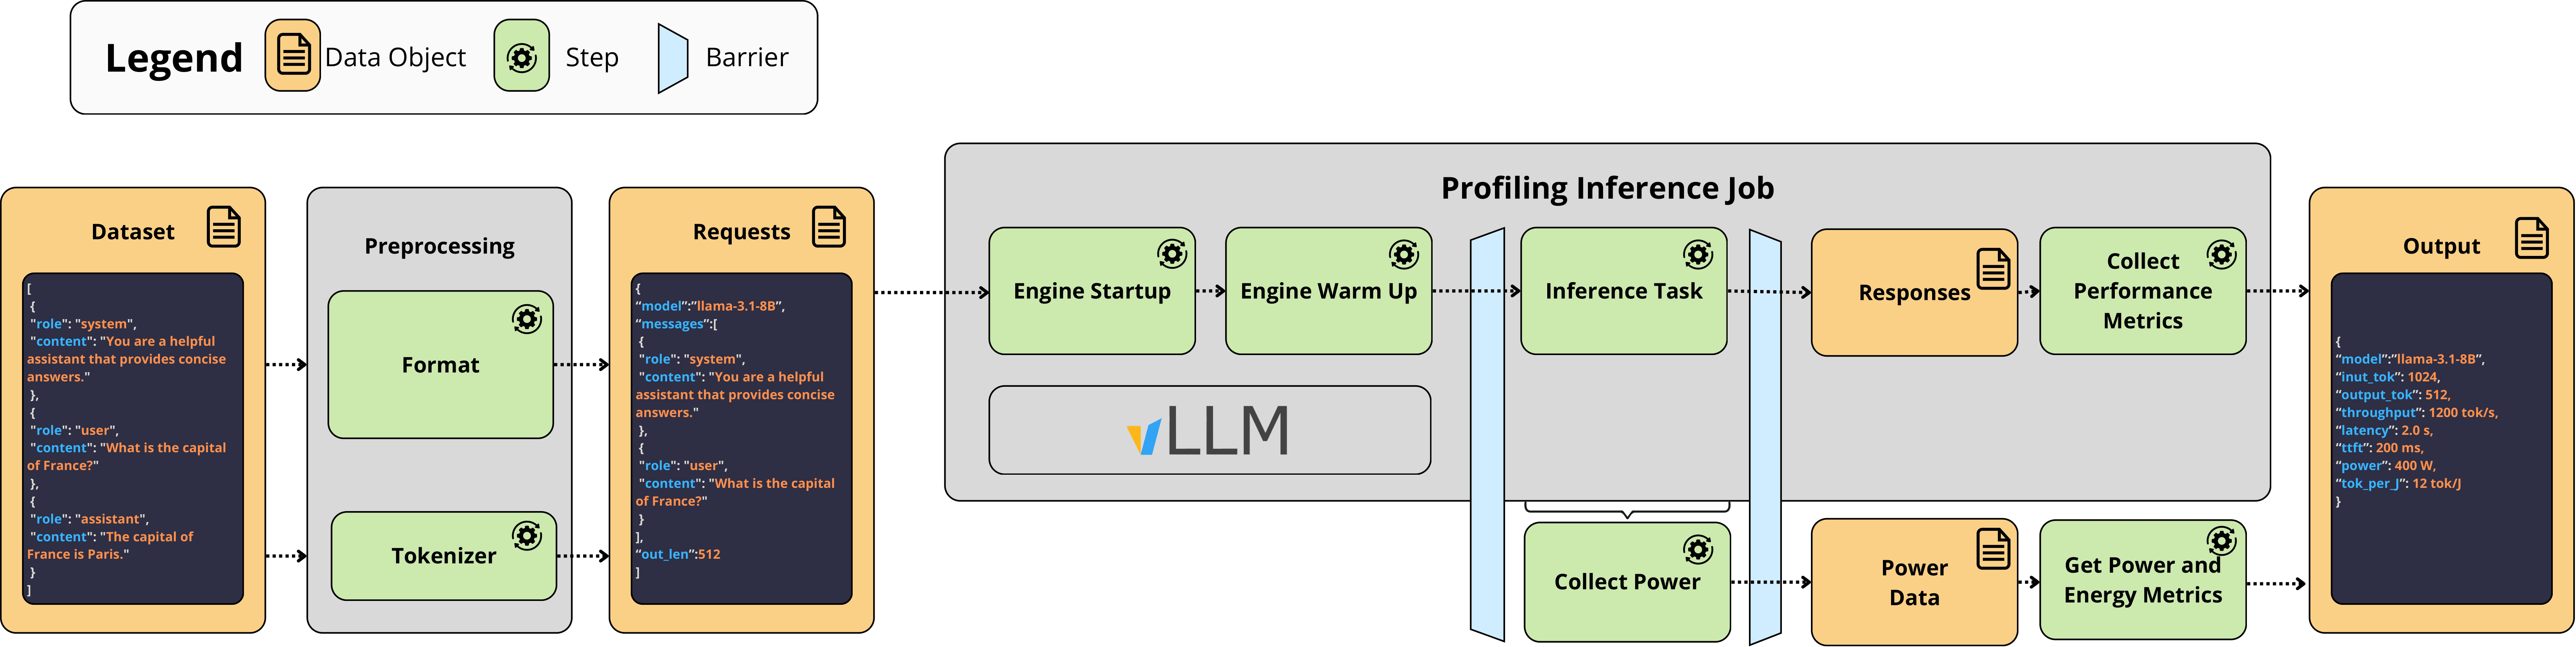
\includegraphics[width=\textwidth]{figs/profile single.png}
    \vspace{5mm}
    \caption{LLM Inference Benchmark Stages.}
    \tagpdfsetup{alttext={LLM Inference Benchmark Stages.}}
    \label{fig:bench}
\end{figure}

To fairly compare those devices, we use a similar software stack on each machine. In particular, we use vLLM \cite{kwon2023efficient}, a high-performance, open-source LLM inference framework compatible with Nvidia, AMD, and Intel GPUs. vLLM allows to achieve superior performance and energy efficiency \cite{fernandez2025energy} compared to the standard Transformers \cite{wolf2019huggingface} implementation by leveraging some key optimizations like the FlashAttention Backend \cite{dao2022flashattention}, PagedAttention \cite{kwon2023efficient}, and continuous batching \cite{agrawal2023sarathi}.
\ref{tab:nodes} reports the specific software stack used on each machine, including the GPU driver, PyTorch version, and vLLM version.

\begin{table}[h!]
\centering
\footnotesize
\caption{GPU nodes used in the experimental evaluation.}
\label{tab:nodes}

\begin{tabularx}{\textwidth}{l l c c c X}
\toprule
\textbf{Vendor} & \textbf{Name} & \textbf{Precision} & \textbf{GPUs/Node} & \textbf{Driver} & \textbf{Software} \\
\midrule

\textbf{NVIDIA} & \textbf{A100}  & BF16, W8A16 & 8  & CUDA 12.6 & \makecell[l]{Torch 2.7.0 \\ vLLM 0.9.0} \\

\textbf{NVIDIA} & \textbf{H100}  & BF16, W8A8  & 4  & CUDA 12.6 & \makecell[l]{Torch 2.7.0 \\ vLLM 0.9.0} \\

\textbf{NVIDIA} & \textbf{GH200} & BF16, W8A8  & 1  & CUDA 12.9 & \makecell[l]{Torch 2.7.0 \\ vLLM 0.9.0} \\

\midrule

\textbf{AMD} & \textbf{MI250}  & BF16        & 4 & ROCm 5.3 & \makecell[l]{Torch 2.7.0+rocm \\ vLLM 0.9.1} \\

\textbf{AMD} & \textbf{MI300X} & BF16, W8A8  & 8 & ROCm 5.3 & \makecell[l]{Torch 2.7.0+rocm \\ vLLM 0.9.1} \\

\midrule

\textbf{Intel} & \textbf{MAX 1550} & FP16 & 6 & oneAPI 2025.2.0 & \makecell[l]{Torch 2.8.0a0 \\ vLLM 0.10.1.xpu} \\

\bottomrule
\end{tabularx}
\end{table}

Each experiment starts by initializing the vLLM engine and loading the inference dataset.
Once the model is loaded and the inference engine is ready, we create an independence process that probes the vendor system monitoring interfaces (py3nvml for NVIDIA, amdsmi for AMD, and xpu-smi for Intel) at consistent intervals to capture power consumption, memory usage, and GPU utilization. For NVIDIA and AMD devices, we sample every 0.5 seconds. For Intel, we have an average sampling rate of 1.9 seconds, due to the longer response time of xpu-smi.
We created the profiler and submitted the inference dataset as a unique batch job to the engine using the vLLM chat method.
Once vLLM has generated the replies for each entry of the dataset, it returns an output object containing information about the end-to-end latency, time to first token, and input and output length of each sequence. This information allows us to collect all the performance metrics described in Section \ref{chap:methods:sec:metrics}.
The profiler data, on the other hand, is used to collect power and energy consumption. To ensure that the profiler process probes the GPU's SMIs only when the GPU is active, we synchronize it with the main process using Python multiprocessing barriers.

For each GPU, this experiment uses different models, precisions, and batch sizes.

Concerning the models, we us four open-source models with a size that ranges from 8B to 32B parameters. Precisely, Llama 3.1 8B, Qwen3 14B, Mistral Small 3.1 24B, and Qwen3 32B. The architectural details of those models are reported in \ref{tab:models}, in the next section.

To evaluate different precisions, we rely on vLLM dynamic weight quantization, which allows us to perform W8A16 quantization (8-bit weights and 16-bit activations) or W8A8 quantization (8-bit weights and 8-bit activations) \cite{vllm-fp8-docs-v0_5_4}, depending on the hardware architecture.
On NVIDIA H100 and AMD MI300x, which offer in-hardware support for FP8 quantization, we use W8A8 quantization. On Nvidia A100, instead, we employ W8A16. Other devices are not included in those experiments, as they do not support either.
For the 16-bit precision, we use bfloat16 (Brain Float 16) precision on Nvidia and AMD, as it is the default precision of the models. For Intel instead, we convert to FP16; single-key optimizations are not yet supported for bfloat16 precision.
Finally, we repeat each experiment for batch sizes of 16 to 128.
\subsection{Multi GPU Experiments}
\label{chap:methods:sec:multi}

We further evaluate LLM inference on GPUs by scaling out to multi-GPU inference.

Multi-GPU parallelism allows for expanding the evaluation in two directions: first, it enables evaluation of significantly larger models compared to single-GPU, thanks to model weight sharding across devices. This also allows a further study of performance scaling with model size. To do so, we include all the models presented in \ref{tab:models}.
Second, as discussed in Section \ref{chap:background:sec:serving}, multi-GPU inference can be implemented using several parallelization strategies, including Tensor Parallelism, Expert Parallelism, and Data Parallelism. As detailed in Section \ref{chap:methods:sec:multi}, these techniques increase the system’s parallel throughput and memory bandwidth approximately linearly with the number of accelerators. Combining these methods introduces a trade-off between the lower communication overhead of Data Parallelism and the greater available memory provided by Tensor Parallelism.

\begin{figure}[h!]
    \centering
    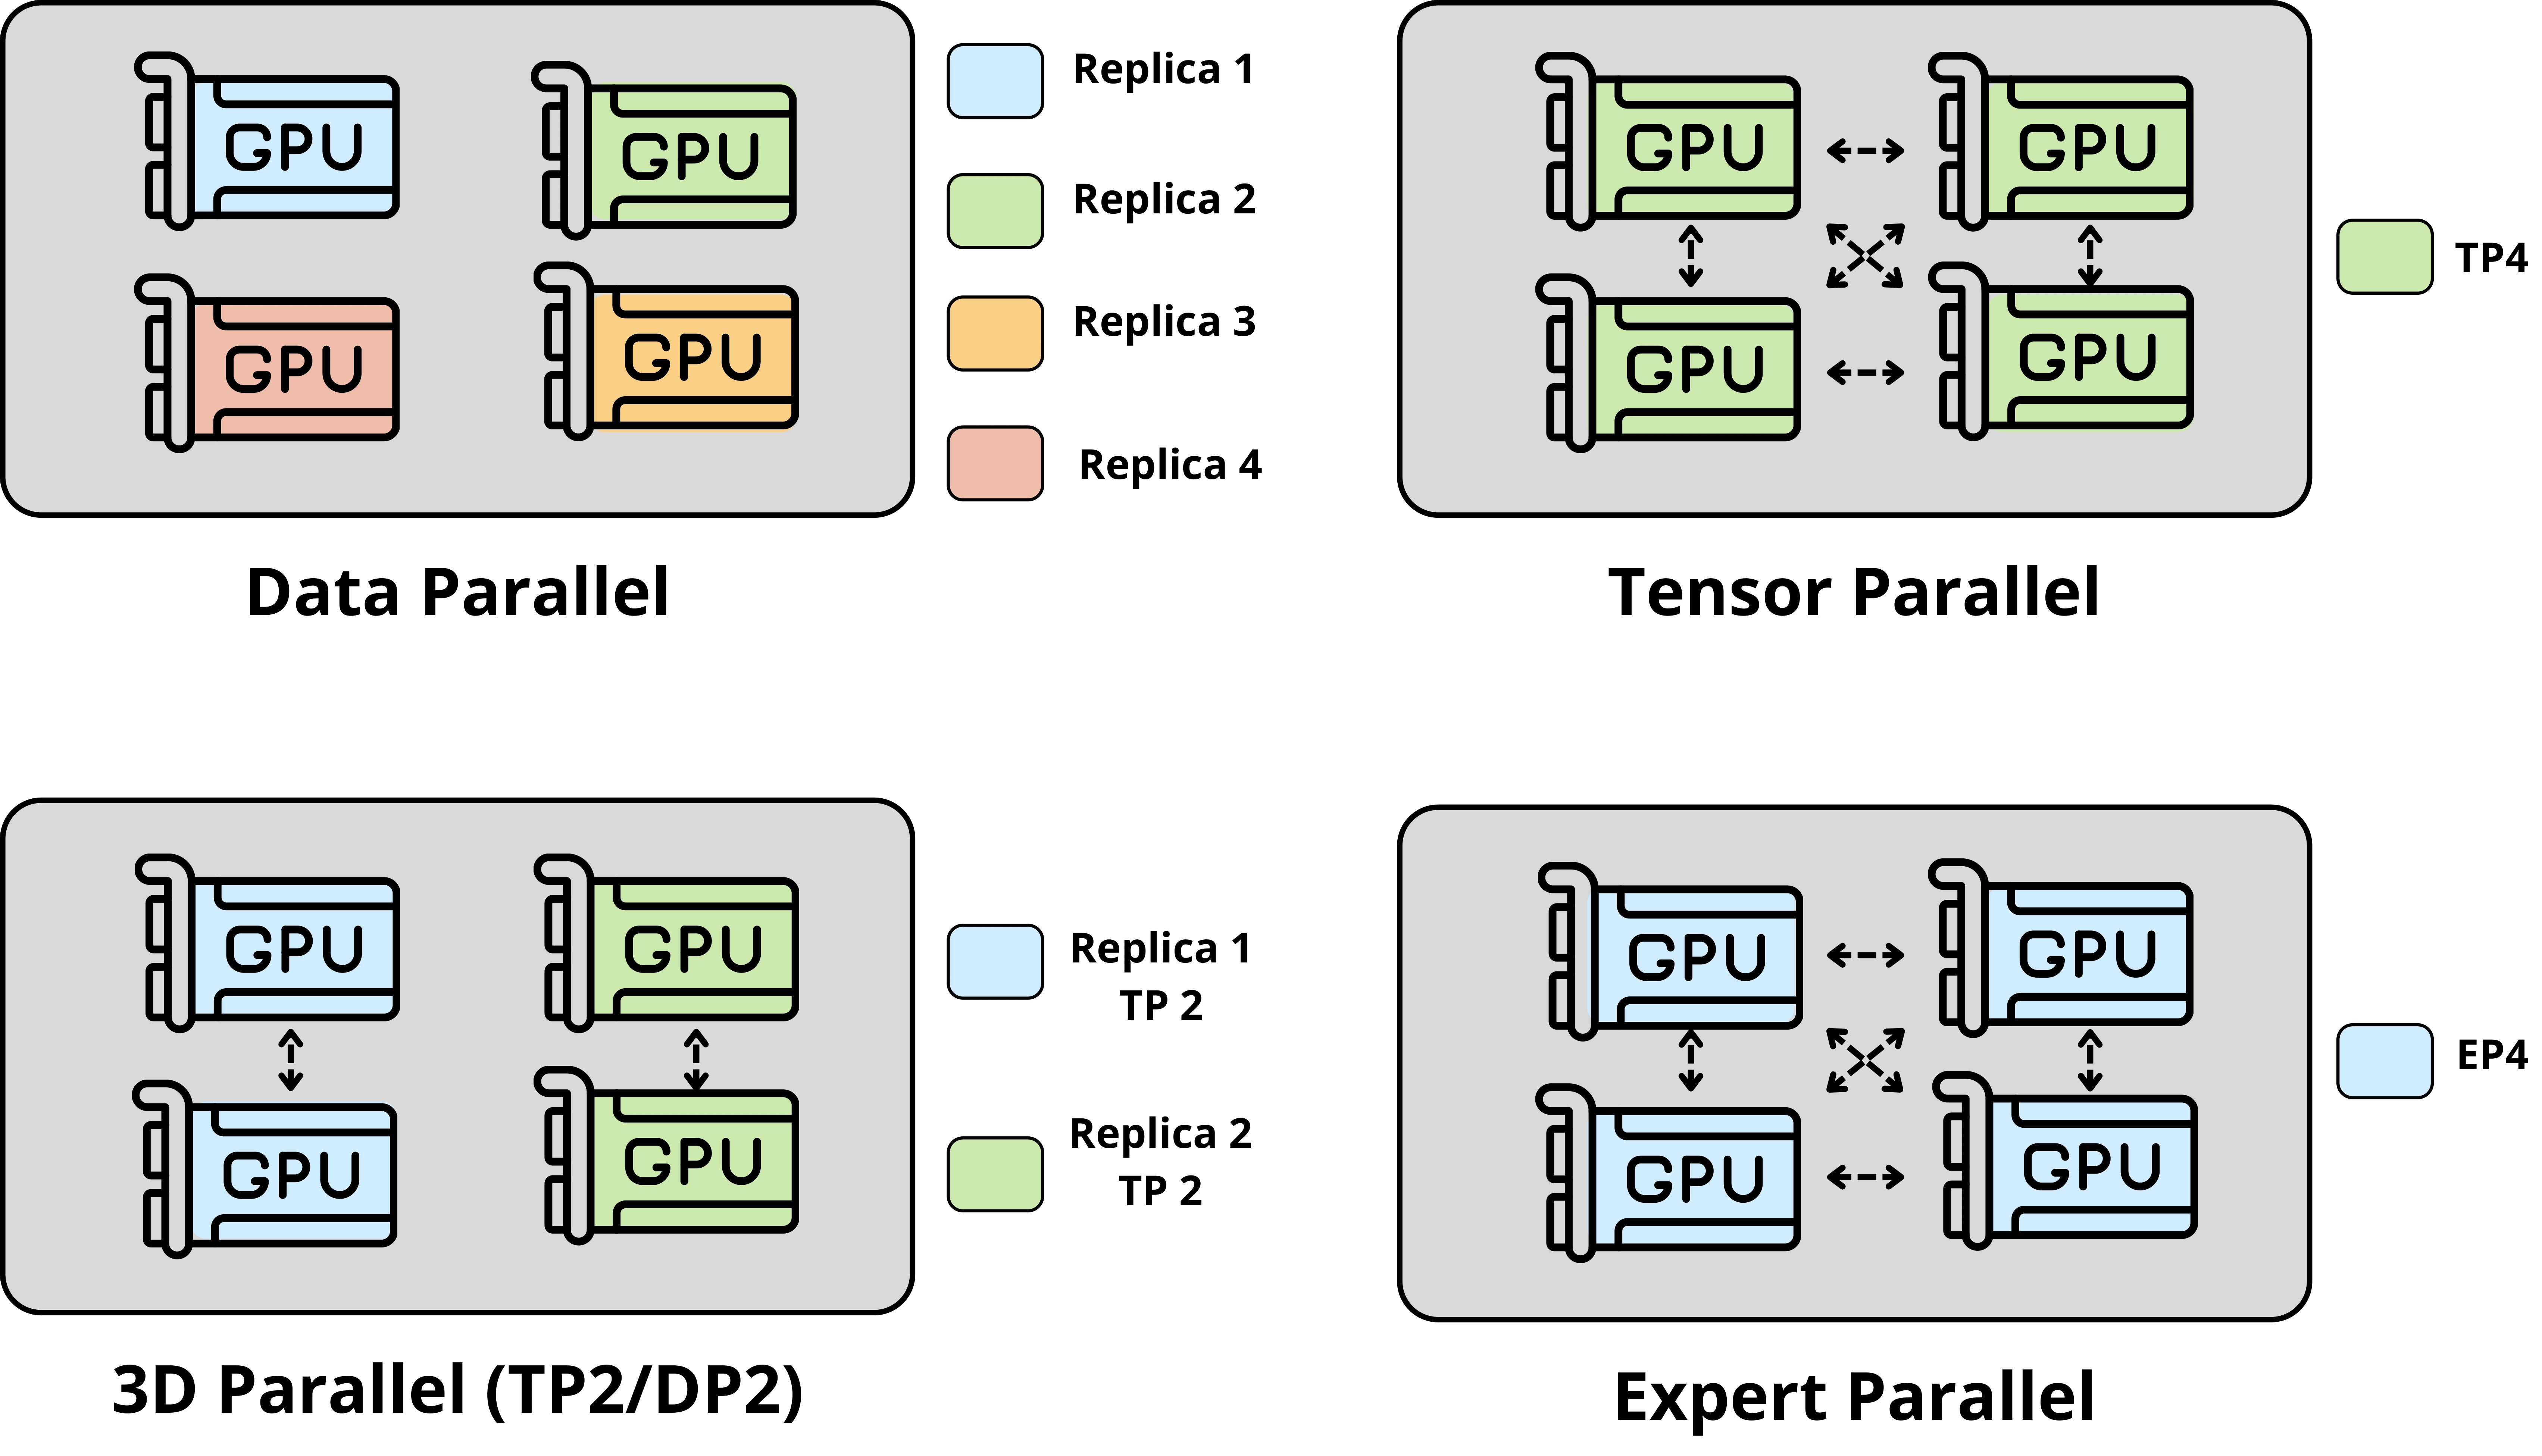
\includegraphics[width=0.85\textwidth]{figs/partition.png}
    \vspace{5mm}
    \caption{Partitioning a node with 3D parallelism.}
    \tagpdfsetup{alttext={Partitioning a node with 3D parallelism.}}
    \label{fig:partition}
\end{figure}

Achieving optimal node-level performance thus requires balancing the number of Data Parallel (DP) replicas and the Tensor Parallel (TP) width per instance, depending on the model size and hardware characteristics. In this study, we explore various TP/DP configurations to empirically determine near-optimal settings. \ref{fig:partition} shows multiple options for partitioning the resources of a 4-GPU node.

\begin{figure}[h!]
    \centering
    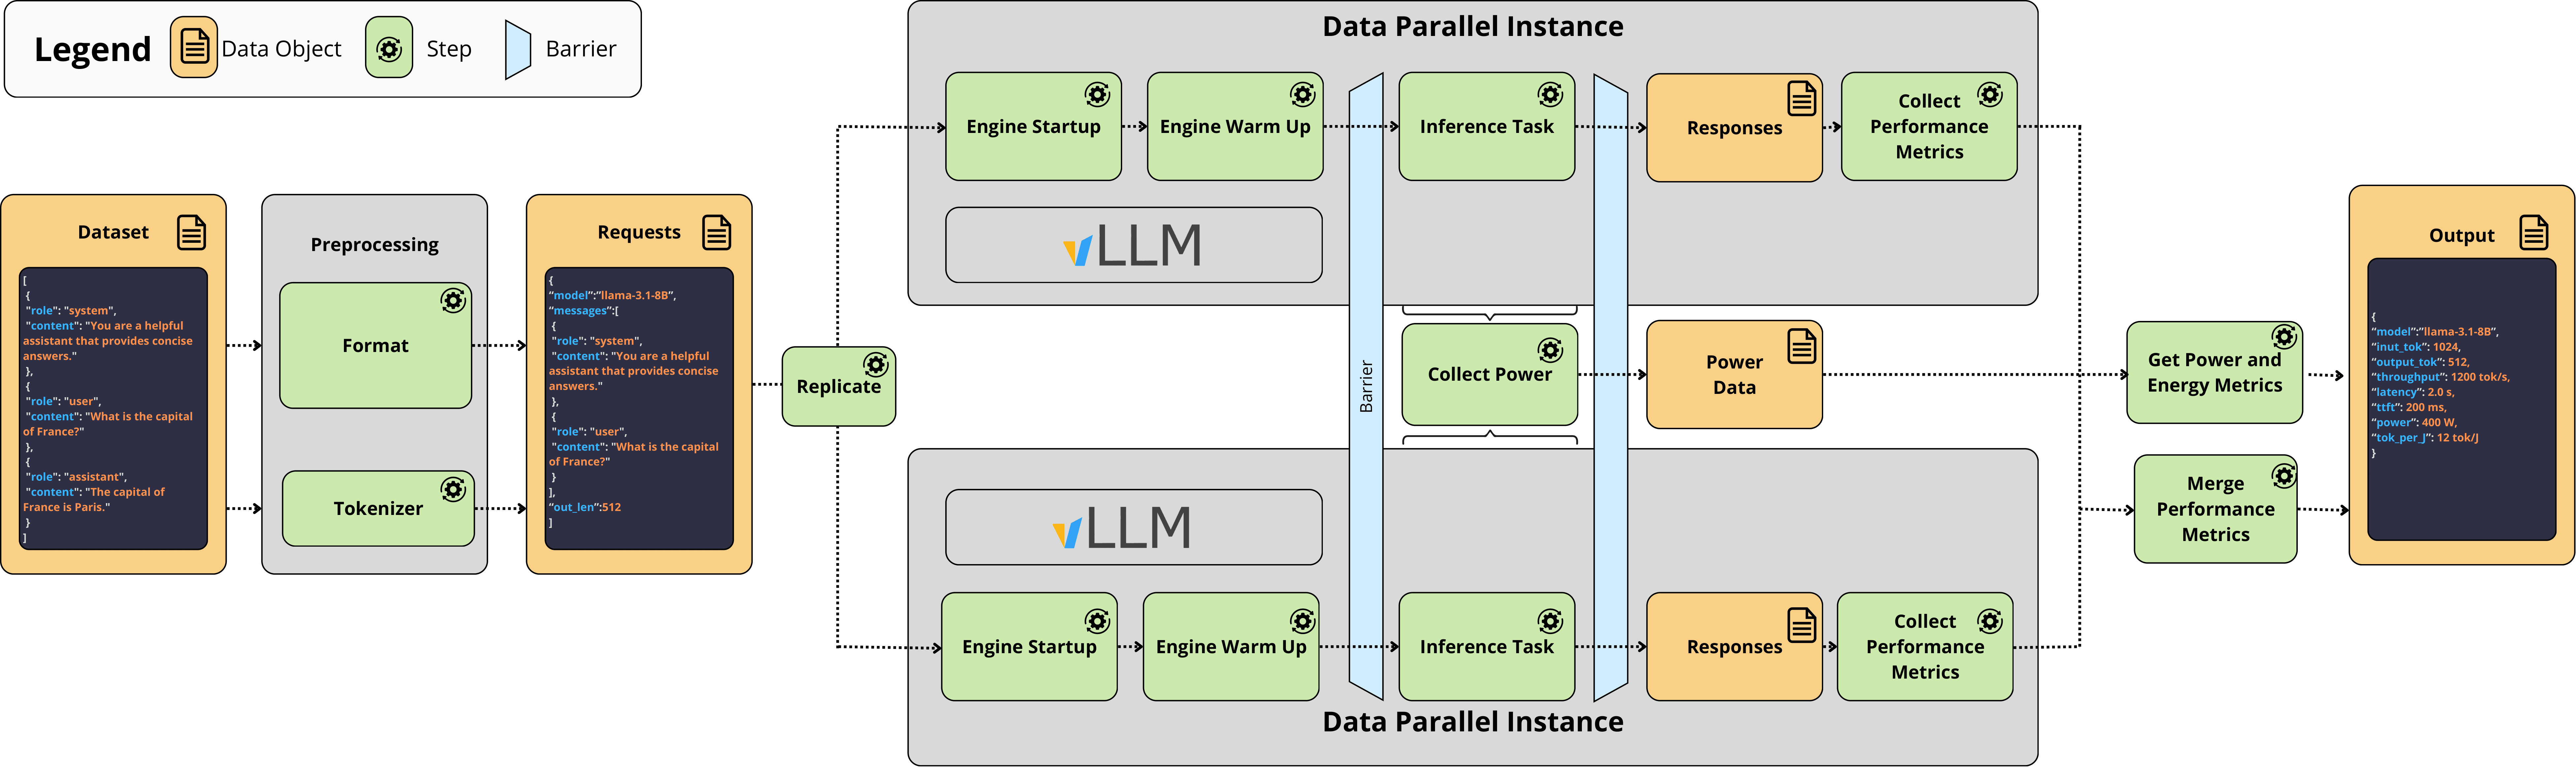
\includegraphics[width=\textwidth]{figs/profile multi.png}
    \vspace{5mm}
    \caption{LLM Inference Benchmark Stages. Multi-GPU setup.}
    \tagpdfsetup{alttext={LLM Inference Benchmark Stages. Multi-GPU setup.}}
    \label{fig:bench}
\end{figure}

An experiment with Data Paralle Size $D$ and Tensor Parallel Size $T$ begins by creating $D$ worker processes and one profiler process. Similar to the single-GPU setup, the profiler process probes the vendor-specific system monitoring interface at consistent intervals to retrieve power consumption data.
Each worker process, instead, initiates a vLLM instance with Tensor Parallel Size $T$. Setting $T\times D = N$, where $N$ is the number of GPUs of the node, allows for an even partition into $D$ homogenous portions, as shown by \ref{fig:partition}.

Once all the $D$ instances are ready, each one starts processing a full instance of the dataset, scaling the single-GPU experiment weakly. When all instances have finished generating replies, their outputs are combined to extract performance metrics, and the profiler process is terminated.

We repeat this experiment with Tensor Parallel Size $T \in \{1, 2, 4\}$ on three multi-GPU nodes: one Sophia bigmem node, featuring 8 DGX A100 80GB GPUs, and two JLSE testbed nodes, featuring 4 NVIDIA H100 SXM5 and 8 AMD Instinct MI300X, respectively. The Data Parallel Size $D$ is set to fully utilize the node. 
The global batch size is set to $128 \times N$, meaning that each of the $D$ instances has a batch size of $128\times T$.
We evaluate both bfloat16 precision and FP8 quantization, using W8A8 on Nvidia H100 and AMD MI300x, and W8A16 on Nvidia A100.

These weak scaling settings allow us to have cleaner performance scaling in two ways. First, it maintains consistency in context lengths across data-parallel instances, since all replicas process identical sequences. Second, it maintains a constant batch size per GPU, ensuring that the number of generated tokens per forward pass remains unchanged across different TP/DP configurations.

\subsection{Comparing Tensor and Expert Parallelism}

We further investigate parallelization strategies for Mixture-of-Experts (MoE) models by comparing Tensor Parallelism (TP) and Expert Parallelism (EP).

Our evaluation includes four large MoE models — Llama4 Scout, Mixtral 8×22B, Qwen 235B A22B, and DeepSeek R1 — all tested in FP8 precision on NVIDIA H100 and AMD MI300x nodes.

Experiments are conducted across varying batch sizes, using a single instance (Data Parallel size = 1) with four GPUs per instance. We first test with a Tensor Parallel size of 4, followed by an Expert Parallel size of 4. The profiling methods used are consistent with those employed in the previous experiment. For DeepSeekR1, we also experimented with 8 GPUs.

\subsection{Dataflow Accelerators Experiments}
\label{chap:methods:sec:dsa}

We investigate LLM inference on hardware accelerators using two dataflow machines: a SambaNova Systems SN40L-16R node \cite{Prabhakar2024}, featuring 16 4th-generation RDUs, and a Cerebras CS3 system \cite{Lie2023} featuring the third-generation Wafer Scale Engine (WSE3). The details of those accelerators are discussed in Section \ref{chap:background:sec:dflow}.

While GPUs are characterized by many streaming multiprocessors that share a common hierarchical memory, dataflow accelerators feature a tiled array of interconnected processing elements, allowing for the mapping of computational graphs into the hardware fabric. This dataflow approach enables reliance solely on fast local scratchpad memories and explicit communication between cores, rather than using a hierarchical cache system as in GPUs, thereby reducing the latency of memory accesses.

Unlike the GPU experiments, which all leveraged vLLM, we utilize a different proprietary inference framework for each dataflow accelerator.

For the Cerebras CS3 system, we use an early-prototype proprietary inference engine that can be queried through an OpenAI-style API.
We task the engine with processing the entire inference dataset by creating one request per conversation.
The Cerebras inference engine supports running models that host weights, activations, and KV caches entirely in on-chip memory to achieve optimal performance. Compared to the streaming-weight approach used for training, this limits the memory capacity to 44GB per CS3 system. For this reason, we limit our analysis to  Llama 3.1 8B.

We repeat the experiment for different batch sizes, ranging from 1 to 8.
To match the engine's effective batch size, we instantiate a corresponding number of clients that send a new request immediately after receiving a response, with the dataset evenly partitioned across clients.
The latencies reported in the responses sent to clients are used to obtain performance metrics.

Regarding power, we collect measurements at the WSE chassis level for all power readings, including the power drawn by the host CPU, WSE, and other supporting components.

For the SambaNova SN40L, we use the SambaStudio inference engine, which can be queried through an OpenAI-compatible interface. Similar to the Cerebras CS3 experiments, we evaluate batch sizes from 1 to 8, creating a number of clients to match the engine's effective batch size.
For this accelerator, we evaluate both Llama 3.1 8B and Llama 3.3 70B.

Regarding power readings, we rely on the PDU-level power consumption for each RDU.
\chapter{Results}
\label{chap:results}

In this chapter, we present the experimental results of our performance and energy-efficiency evaluation of modern datacenter AI accelerators. Following the structure introduced in Chapter~\ref{chap:methods}, we organise the discussion into three parts: Single-GPU experiments (Section~\ref{chap:results:sec:single}), Multi-GPU experiments (Section~\ref{chap:results:sec:multi}), and an analysis of dataflow AI accelerators (Section~\ref{chap:results:sec:dsa}).


\section{Single GPU Experiments}
\label{chap:results:sec:single}

In this section, we discuss the performance of LLM inference on a single GPU, comparing six different GPUs from Nvidia, AMD, and Intel.
We analyze three key performance metrics: End-to-end latency, Time to First Token (TTFT), and Throughput.
For energy efficiency, we utilize Tokens per Joule as the metric.

\ref{fig:all_metrics_1gpu} shows how performance and energy efficiency evolve with batch size across 6 different GPUs and four LLM models running with half (16-bit) precision. Multi-Tile GPUs (AMD MI250 and Intel Max 1550) use tensor parallelism to fully utilize their resources.
From those experiments, we can extract three main insights: 
(1) a cross-vendor comparison of the performance and energy efficiency of GPU models, \
(2) the trend of performance and energy efficiency as model size grows, and 
(3) the trade-off between latency and throughput across different batch sizes.

\begin{figure}[h]
    \centering
    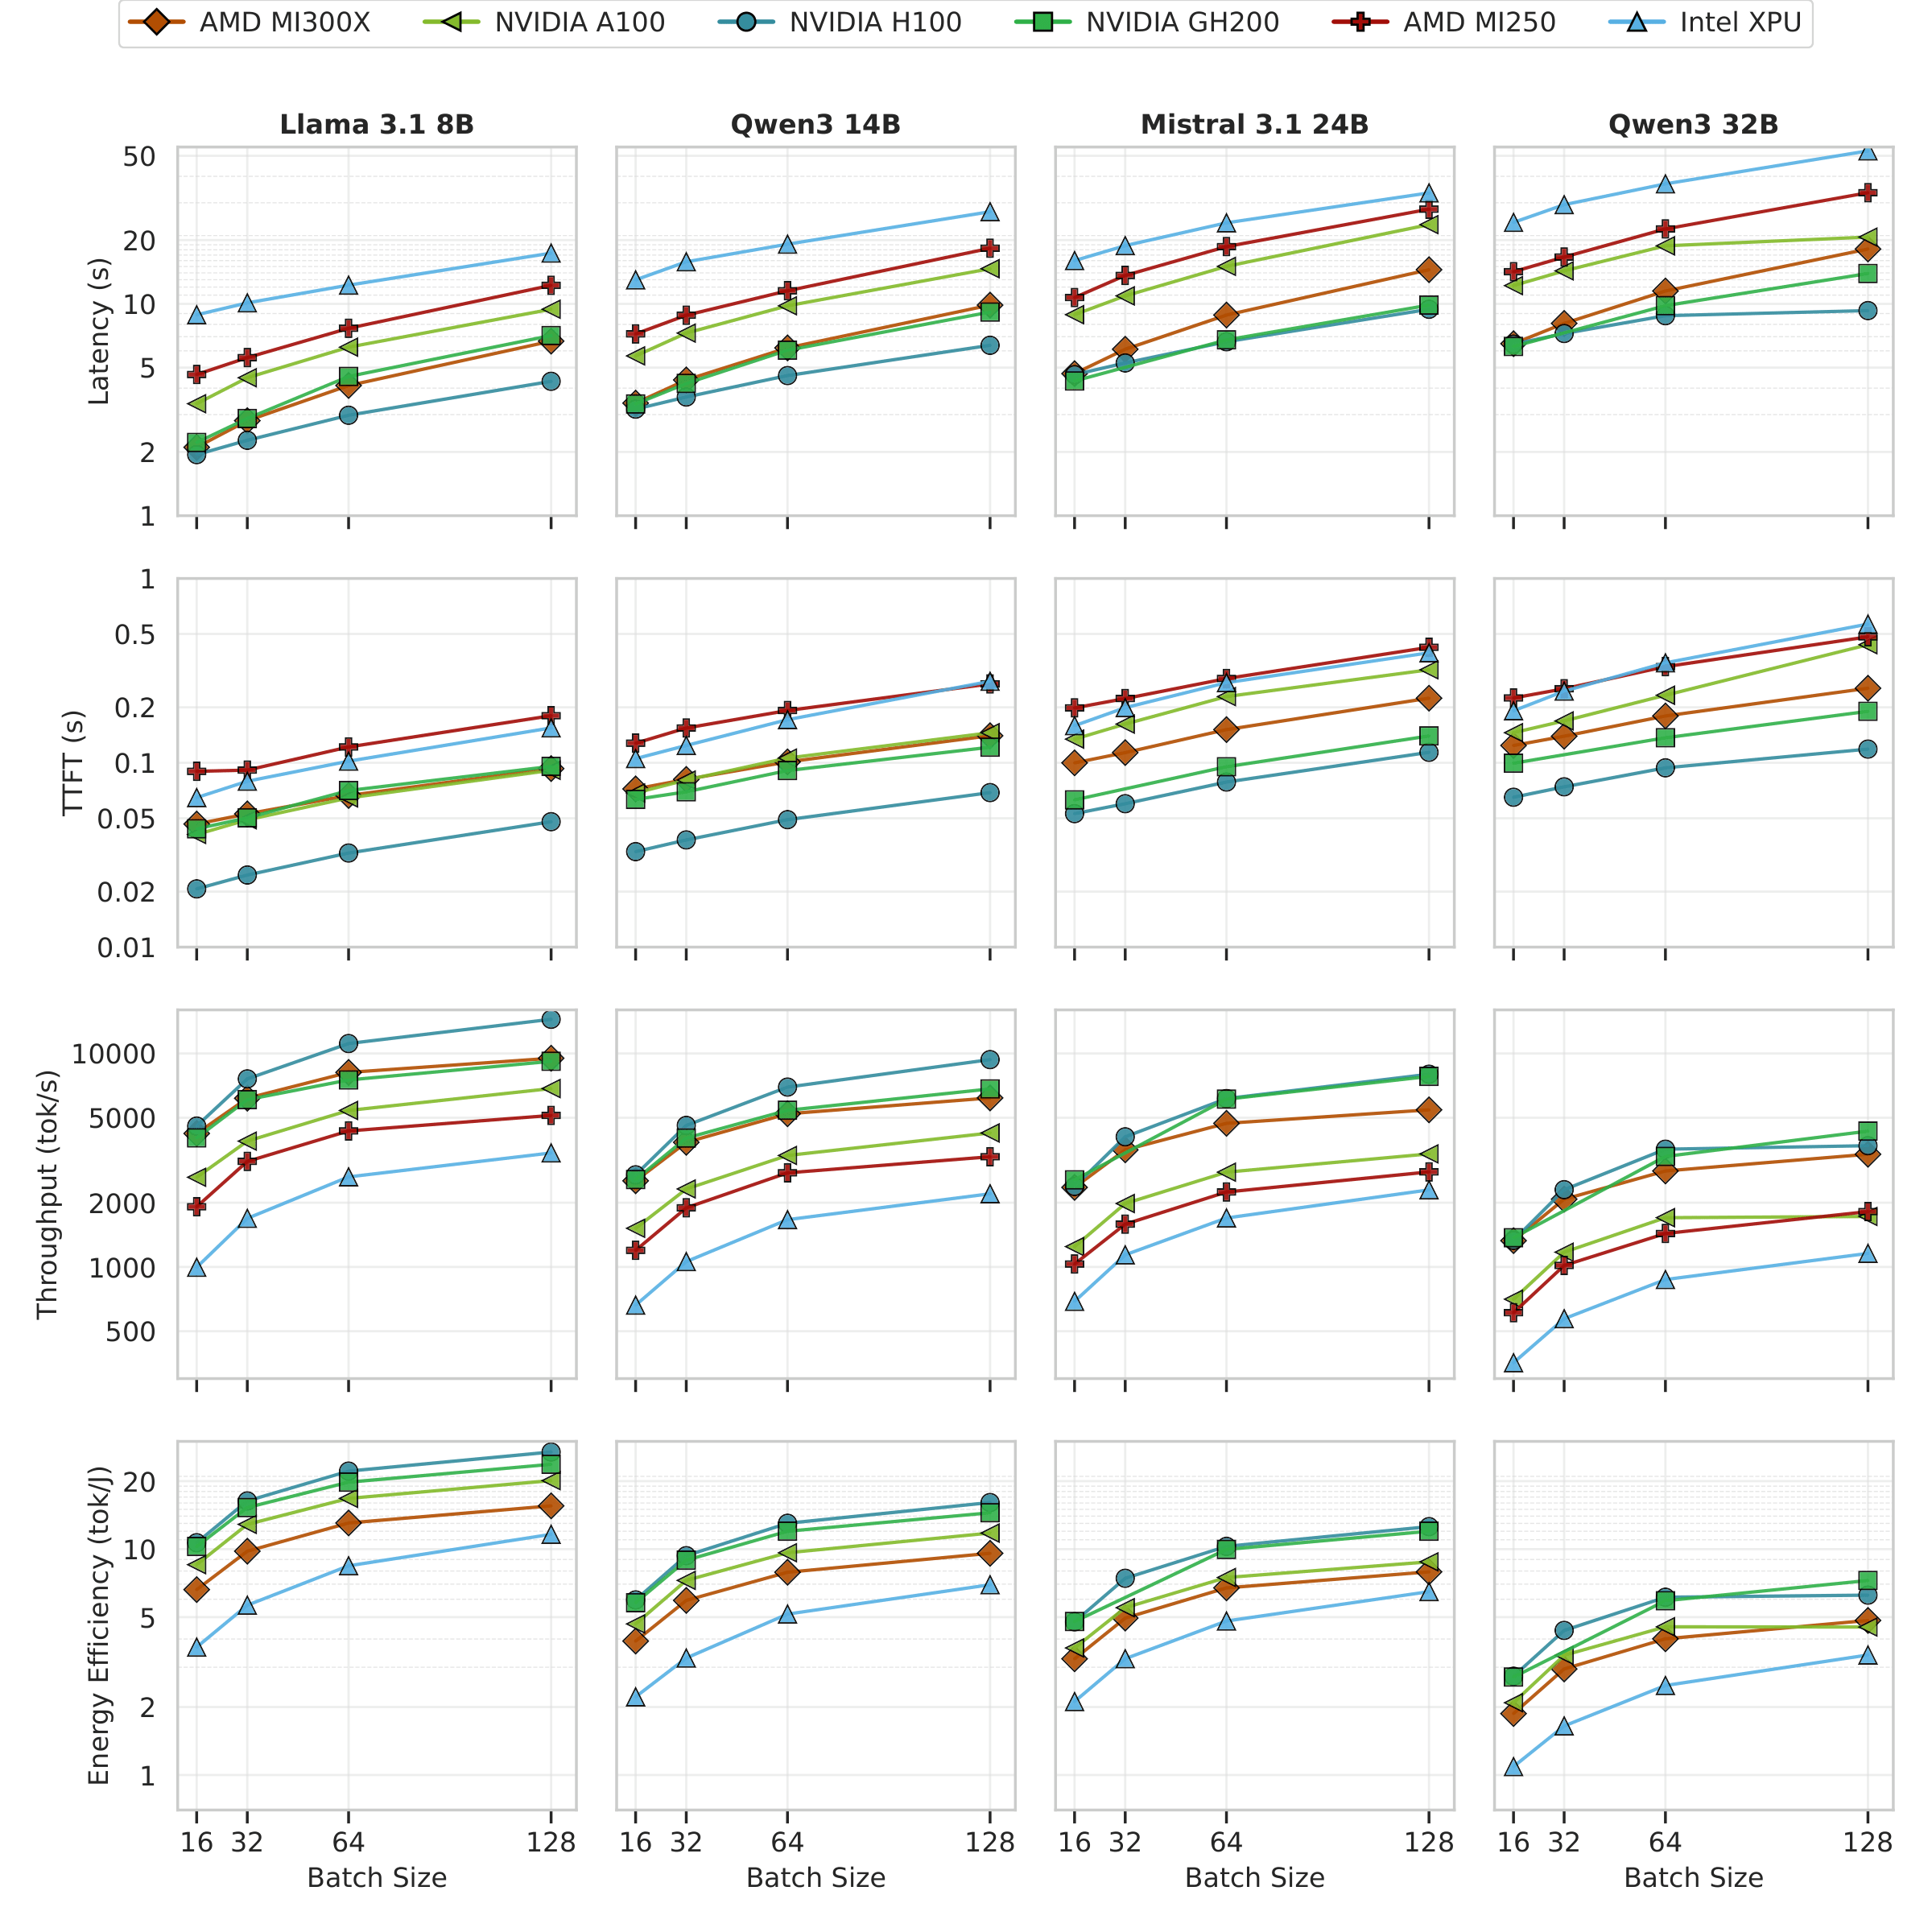
\includegraphics[width=\textwidth]{figs/combined_performance_plots.png}
    \caption{The evolution of performance and energy efficiency with batch size across six GPUs.}
    \tagpdfsetup{alttext={The evolution of performance and energy efficiency with batch size across six GPUs.}}
    \label{fig:all_metrics_1gpu}
\end{figure}

\subsection{GPU model comparison}
For this analysis, we use the NVIDIA A100 as the natural performance baseline, as it is both the oldest and most widely used GPU among those tested. Both Nvidia Hopper (H100 and GH200) and AMD CDNA3 (MI300x) GPUs consistently outperform the A100 baseline in terms of performance, across models and batch sizes. The AMD MI250 and the Intel Max 1550, instead, are both outperformed by the Ampere GPU. Importantly, both GPUs feature larger memories than their Nvidia counterparts (128 GB compared to 80 GB), which leads to two main benefits. First, they support running larger models, and second, they substantially narrow the throughput gap as model size and batch size increase. In fact, especially with the larger 32B model, Nvidia A100 and H100 saturate their throughput at batch size 64 due to the insufficient memory available for KV cache.
Concerning the increased latency and the lower throughput, it is also important to mention that each Intel Max 1550 and AMD MI250 is constituted of two GPU tiles and thus requires frequent all-gather operations between the two to fully utilize its compute power. This is particularly detrimental in small models, advantaging monolithic GPUs.

Regarding energy efficiency, Nvidia Hopper GPUs demonstrate an improvement over the previous generation, despite their increased average power consumption. In fact, where the Nvidia A100 had a TDP of 400W and an average power consumption of 337W, the Nvidia H100 has a TDP of 700W and consumes, on average, 478W. Nevertheless, the substantial decrease in latency is sufficient to compensate for the increased power consumption.
The same does not hold for AMD MI300x, which consistently surpasses the A100 in raw performance but achieves lower energy efficiency. Notably, the AMD MI300x has the highest power consumption among the GPUs tested (750W TDP and 625W average power consumption).
The Intel Max 1550 exhibits higher latency and increased power consumption compared to the Nvidia A100, resulting in lower energy efficiency.

AMD MI250 and Intel Max 1550 underperform relative to the NVIDIA A100 despite their higher power consumption. This gap is partly due to their multi-tile designs, which require tensor parallelism to fully utilize the hardware, as each tile is presented to the operating system as a separate device. Additionally, the AMD and Intel implementations of vLLM currently lag in software maturity, lacking support for key optimizations. In terms of energy efficiency, the Intel Max 1550 is less efficient than the A100, while no data is available for the AMD MI250.

Memory capacity is another critical factor. NVIDIA GPUs rank lowest in VRAM, which limits the size of models they can host compared to the other GPUs under analysis. The AMD MI300x provides the largest memory capacity at 192GB, enabling a single device to run 70B-parameter models. It is also important to note that the current vLLM implementation does not utilize all the unified memory of the GH200 SoC, which limits the memory capacity to 96 GB of VRAM, resulting in comparable performance to the base NVIDIA H100.

NVIDIA Hopper GPUs emerge as the most performant and energy-efficient GPU among those tested. The AMD MI300X also displays competitive performance, outpacing the NVIDIA A100 in terms of performance, but not in energy efficiency. Intel Max 1550 and AMD MI250 offer lower performance and energy efficiency than NVIDIA A100.

\begin{figure}[H]
    \centering
    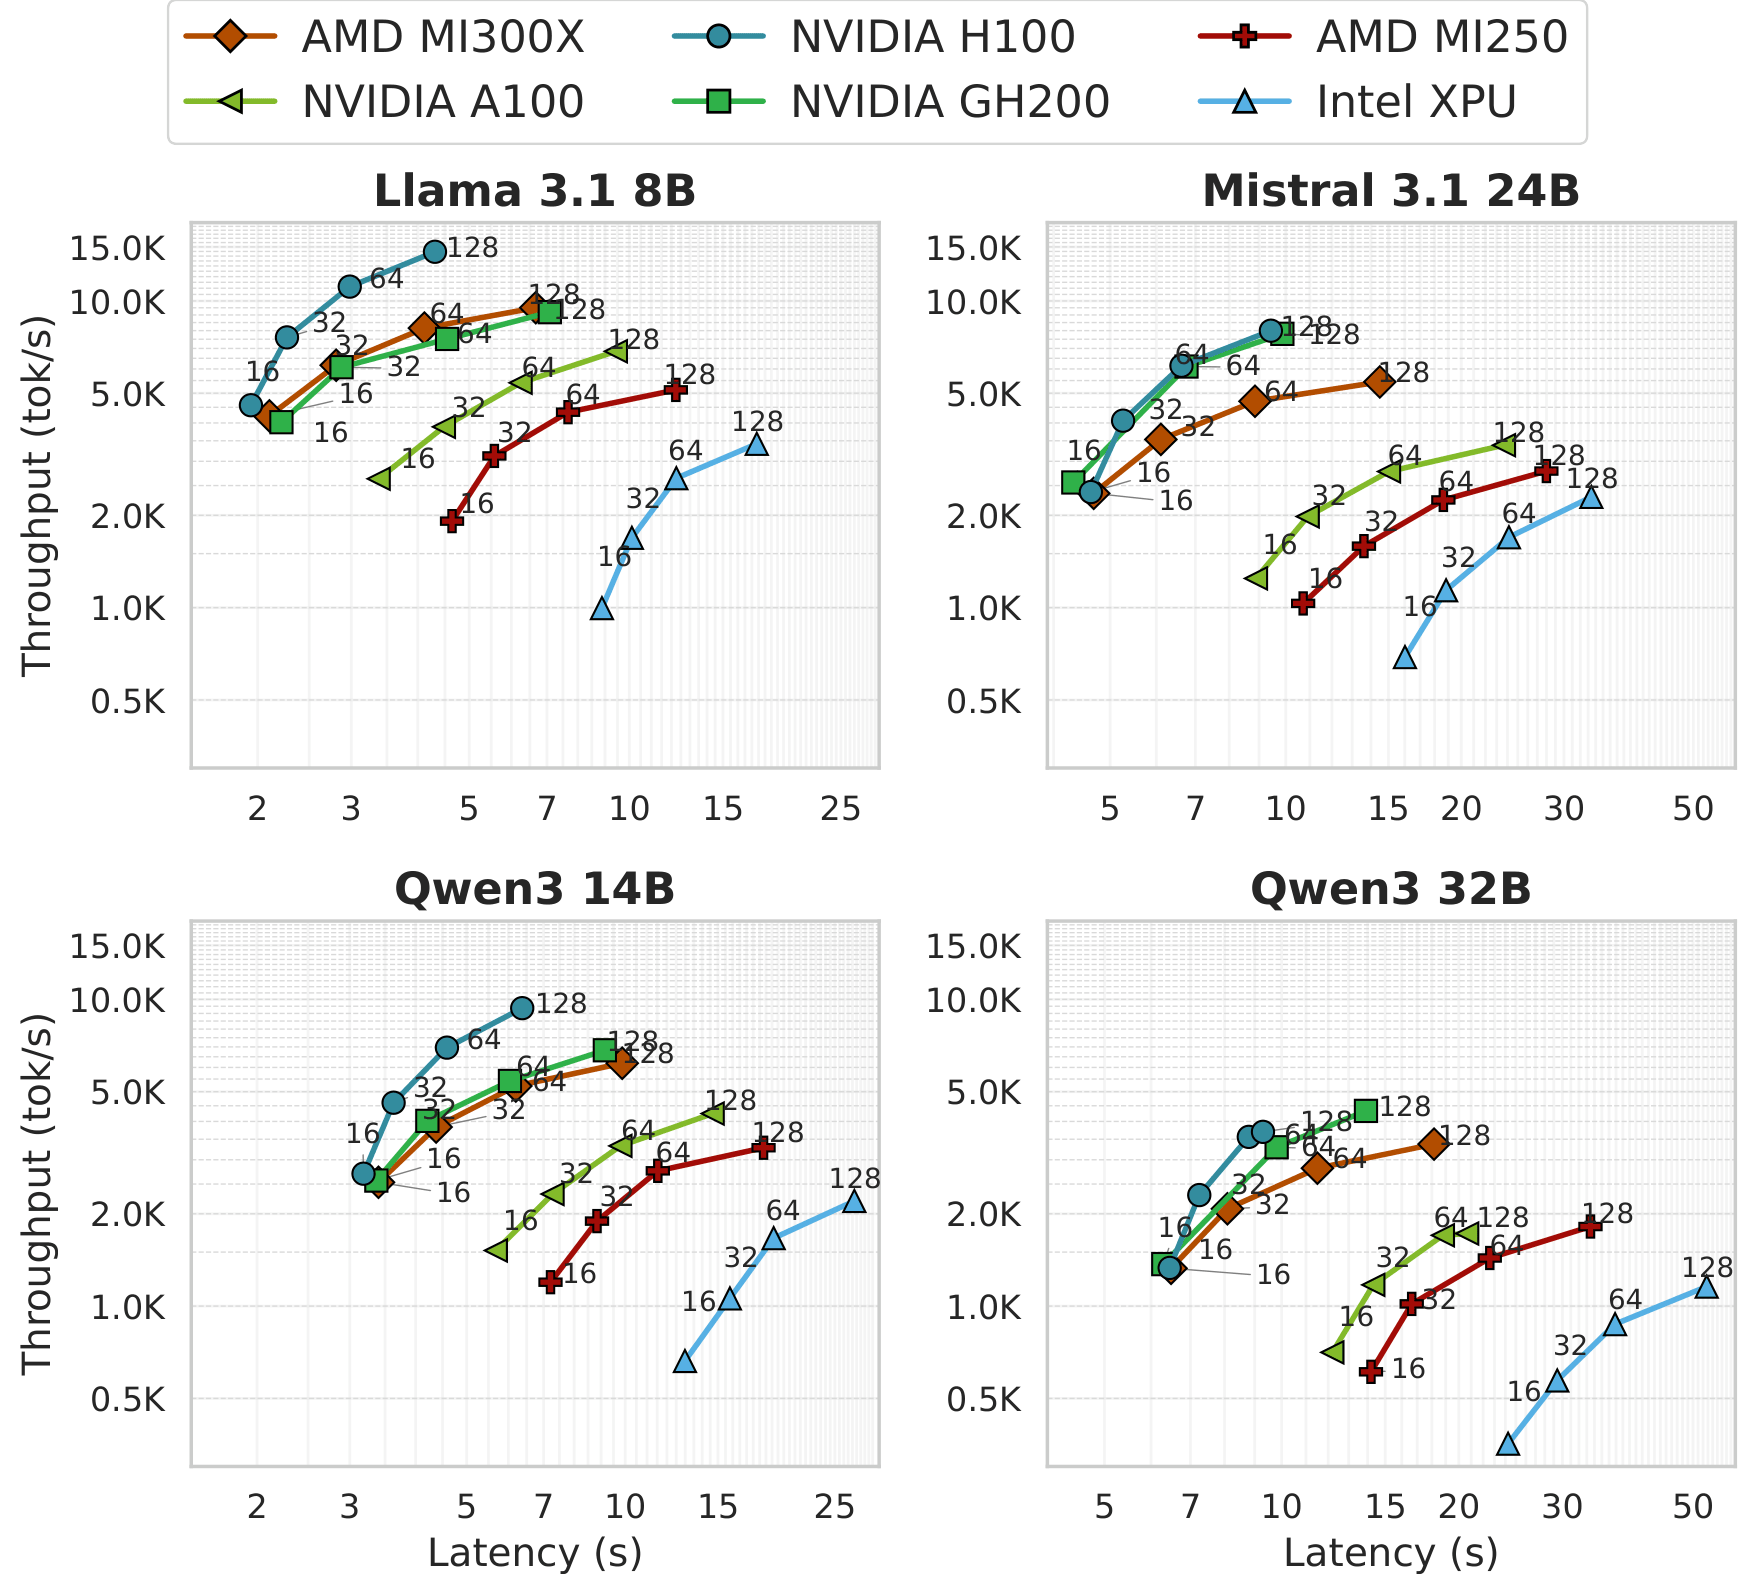
\includegraphics[width=0.9\textwidth]{figs/throughput_latency_plot.png}
        \caption{Trade-off between throughput and latency across batch sizes (16-128), using four LLM models and six different GPUs. The numbers in the plots indicate the batch sizes.}
        \tagpdfsetup{alttext={Trade-off between throughput and latency across batch sizes (16-128), using four LLM models and six different GPUs. The numbers in the plots indicate the batch sizes.}}
    \label{fig:bs}
\end{figure}

\subsection{Batch Size} 
\ref{fig:bs} presents a different perspective on our evaluation data, enabling us to better understand the impact of batch size. The x-axis represents the average end-to-end latency of sequences, while the y-axis represents throughput. These representations allow us to observe the trade-off that happens under varying batch sizes.
Consistent with the analysis in Chapter \ref{chap:methods:sec:model}, we observe that across all GPU models, smaller batches result in lower latency due to reduced computation at each forward pass.
In fact, the number of FLOPs to be executed at each forward pass scales linearly with batch size $b$. However, the model weights have to be loaded from off-chip memory independently of $b$. This causes the compute-related part of latency to decrease linearly with batch size, while the operational intensity $OI$ (expressed in FLOPs/byte) drops linearly with $b$, making computation more memory-bound and thus harming throughput.

Increasing throughput also strongly correlates with improving energy efficiency.
After adjusting the GPU model and precision, we observe a correlation of 0.92 to 0.99 between energy efficiency and throughput. This is because batch size has a reduced impact on power consumption, whereas it has a significant effect on latency.

From these observations, we conclude that larger batch sizes improve the performance in an offline setting while also achieving better energy efficiency.
In contrast, metrics related to online serving, such as TTFT, ITL, or E2E latency, improve as the batch size decreases, creating a trade-off with energy efficiency. 

\begin{figure}[H]
    \centering
    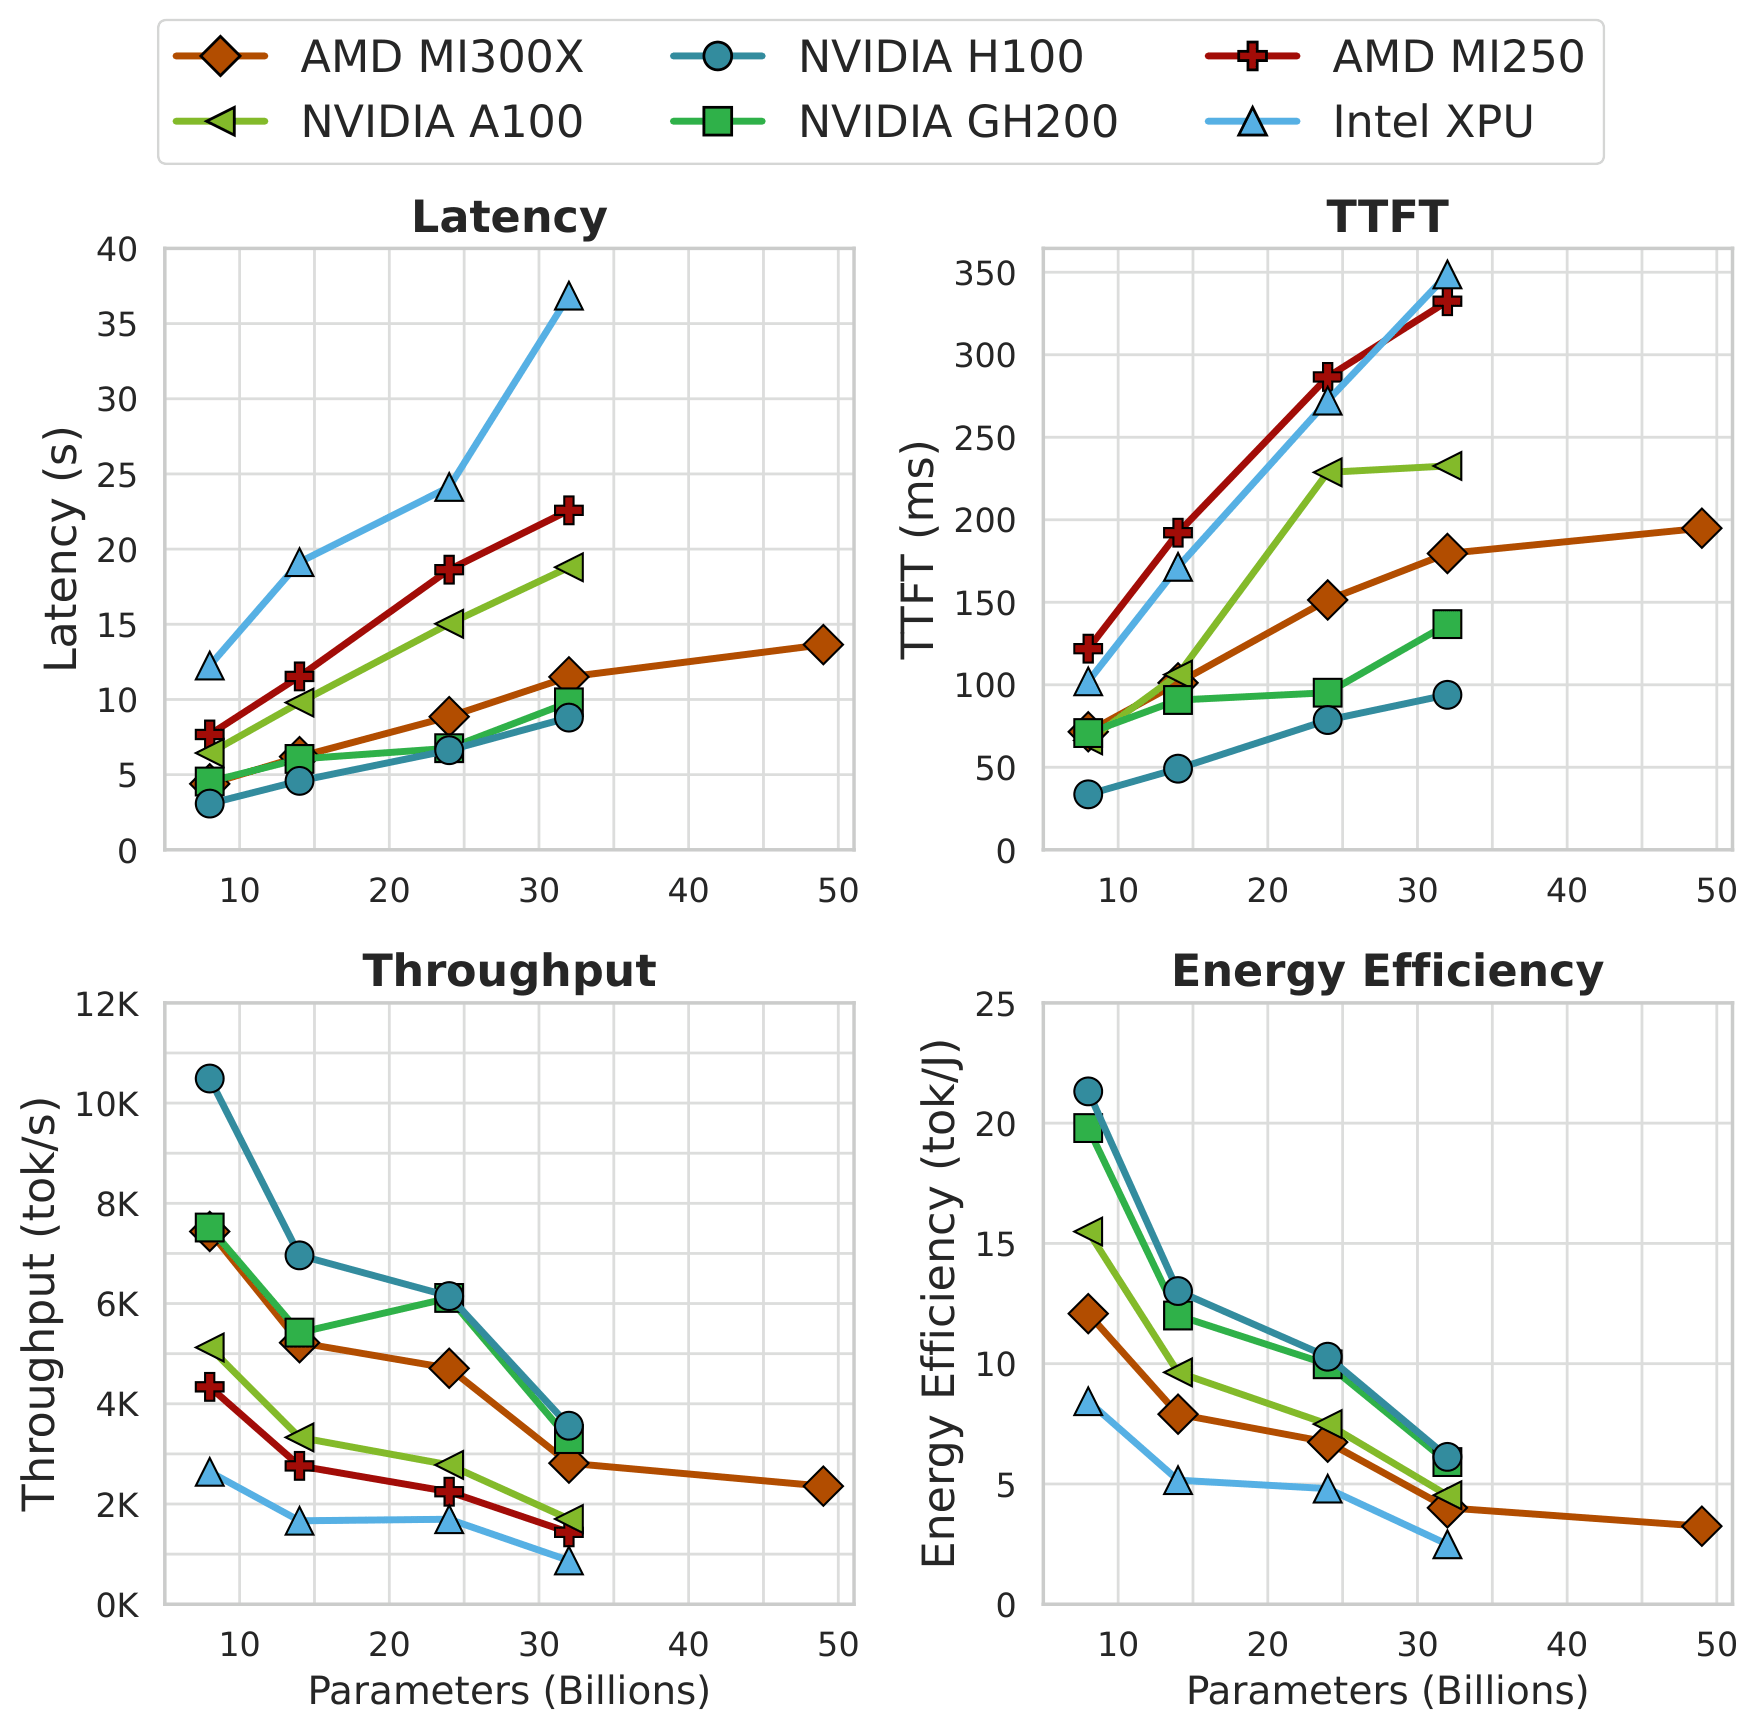
\includegraphics[width=0.7\textwidth]{figs/trend_Latency_TTFT_Throughput_Energy.png}
    \caption{Performance and energy efficiency across six GPUs for models of varying size.}
    \tagpdfsetup{alttext={Performance and energy efficiency across six GPUs for models of varying size.}}
    \label{fig:1gpu_modelsize}
\end{figure}

\subsection{Model Size} 
\ref{fig:1gpu_modelsize} displays a subset of the datapoints from \ref{fig:all_metrics_1gpu}, allowing us to better visualize how the four key metrics analyzed change as the model size increases, with the input dataset and batch size set to 64. 

As a first observation, we can see that latency and TTFT increase linearly with model size, while throughput and energy efficiency decrease inversely.
This trend is consistent with the analysis made in Chapter \ref{chap:methods:sec:model}, which predicts the latency of the forward pass to scale roughly linearly with the model size $N$.

\begin{comment}
\begin{figure}[H]
    \centering
    \includegraphics[width=0.9\textwidth]{figs/fp8_vs_bf16_improvements_subplots.png}
        \caption{  Throughput and energy-efficiency gains (FP8 vs. bfloat16) across four LLM models and four GPUs. The greatest improvement is annotated.}
    \label{fig:fp8}
\end{figure}
\end{comment}

\begin{figure}[H]
    \centering
    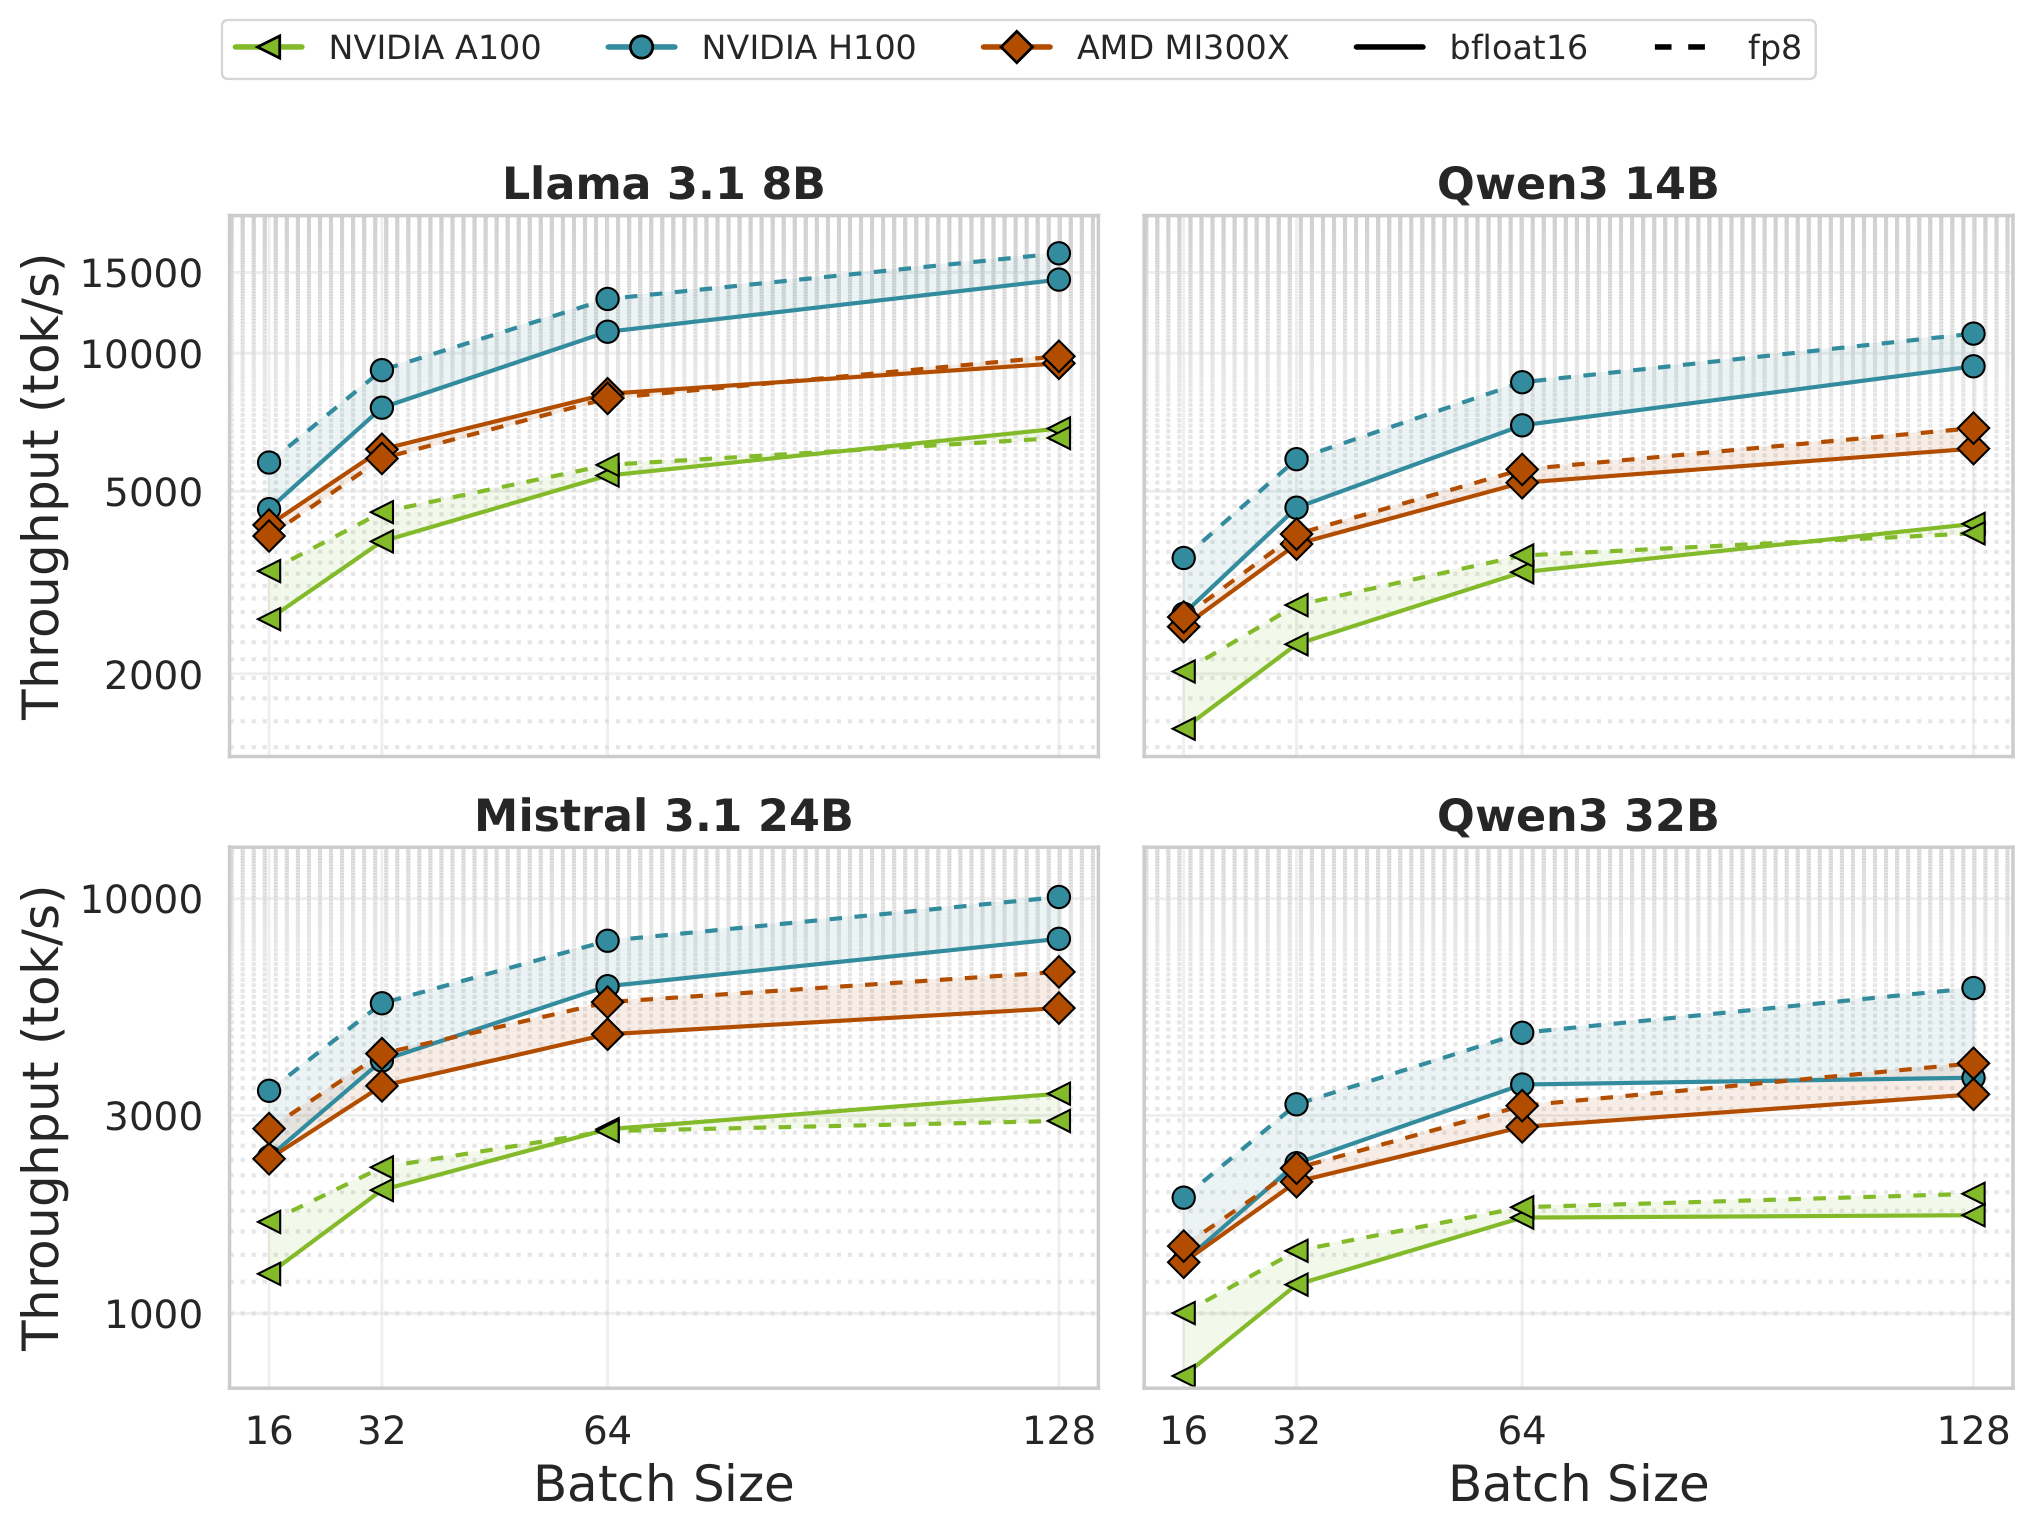
\includegraphics[width=\textwidth]{figs/throughput_by_model_with_precisions_filled.png}
    \caption{Throughput (tok/s) comaprison between bfloat16 and FP8 precision across GPUs and LLM models.}
    \tagpdfsetup{alttext={Throughput (tok/s) comaprison between bfloat16 and FP8 precision across GPUs and LLM models.}}
    \label{fig:fp8bs}
\end{figure}

\subsection{FP8 Quantization}

We evaluate the impact of FP8 quantization on throughput and energy efficiency across four GPU architectures: NVIDIA A100, H100, GH200, and AMD MI300X. \ref{fig:fp8bs} summarizes the results.

NVIDIA A100 does not provide native FP8 support and therefore relies on W8A16 quantization, which applies 8-bit weights and 16-bit activations. Although it cannot exploit FP8-specific functional units, A100 still benefits from the reduced memory footprint of 8-bit weights. In contrast, NVIDIA Hopper (H100, GH200) and AMD MI300X implement FP8 arithmetic natively and can operate with W8A8 precision throughout, yielding more substantial performance gains.

In theory, reducing precision from bfloat16 to W8A8 halves both the arithmetic cost and data movement, suggesting a near 2 $\times$ speedup. In practice, our measurements show that real-world improvements fall well short of this idealized limit. While W8A8 consistently outperforms bfloat16, the magnitude of gains varies significantly across hardware.

NVIDIA Hopper GPUs benefit the most, with throughput improvements of 20\%–38\% and energy-efficiency gains of 34\%–46\%. AMD MI300X shows smaller and more model-dependent improvements: throughput ranges from no gain on Llama 8B to roughly 20\% on Mistral Small 24B; energy efficiency improves by 16\%–35\%. These results highlight the gap between theoretical and practical benefits, underscoring the need for hardware–software co-design to fully exploit low-precision arithmetic.

Batch size also plays an important role. W8A8 quantization becomes increasingly advantageous at larger batch sizes, where arithmetic dominates execution time. Conversely, W8A16 (used on A100) yields its largest gains at small batch sizes, where the workload is more memory-bound, and exhibits diminishing returns as the batch size increases. \ref{fig:fp8bs} illustrates these trends for Qwen3 32B.

Quantization inevitably introduces some loss in model accuracy. While a complete analysis is left for future work, prior results \cite{kurtic2024give} indicate that FP8-quantized models retain more than 99\% of the accuracy of their bfloat16 counterparts on standard benchmarks, suggesting that accuracy degradation is typically minor.

In summary, W8A8 quantization delivers meaningful speedups and energy savings at minimal accuracy cost, with NVIDIA Hopper GPUs achieving the largest benefits (up to 44\% throughput and 47\% energy efficiency). AMD MI300X gains are smaller but often significant for larger models, whereas W8A16 on A100 is most effective at small batch sizes.
\section{Multi GPU Experiments}
\label{chap:results:sec:multi}

In the second part of our evaluation, we examine the performance of multi-GPU inference. We evaluate three multi-GPU nodes featuring 8 NVIDIA A100, 4 NVIDIA H100, and 8 AMD MI300x, respectively.
Each node is tested with three configurations, corresponding to tensor parallel sizes of 1, 2, and 4, and a data parallel size set to fully utilize the node's resources.
Using bfloat16 precision, we evaluate 10 models, while with FP8 quantization, we evaluate 14 LLMs.

The data is presented through two heatmaps (\ref{fig:heatmapbf16} and \ref{fig:heatmapfp8}), structured to have one row per model and three columns per node, corresponding to the different partitions.
The models are sorted by parameter count, while the columns correspond to different models and their TP/DP settings. Throughput is normalized by the number of data parallel instances, while energy efficiency does not need to be normalized due to weak scaling (see \ref{chap:methods:sec:multi}).

This data allows us to observe different trends of multi-GPU inference, including
(1) the scaling efficiency of Data and Tensor Parallelism,
(2) the impact of model size scaling on performance,
(3) a cross-vendor comparison of the three nodes, in a multi-GPU setting.

\begin{figure}[H]
    \centering
    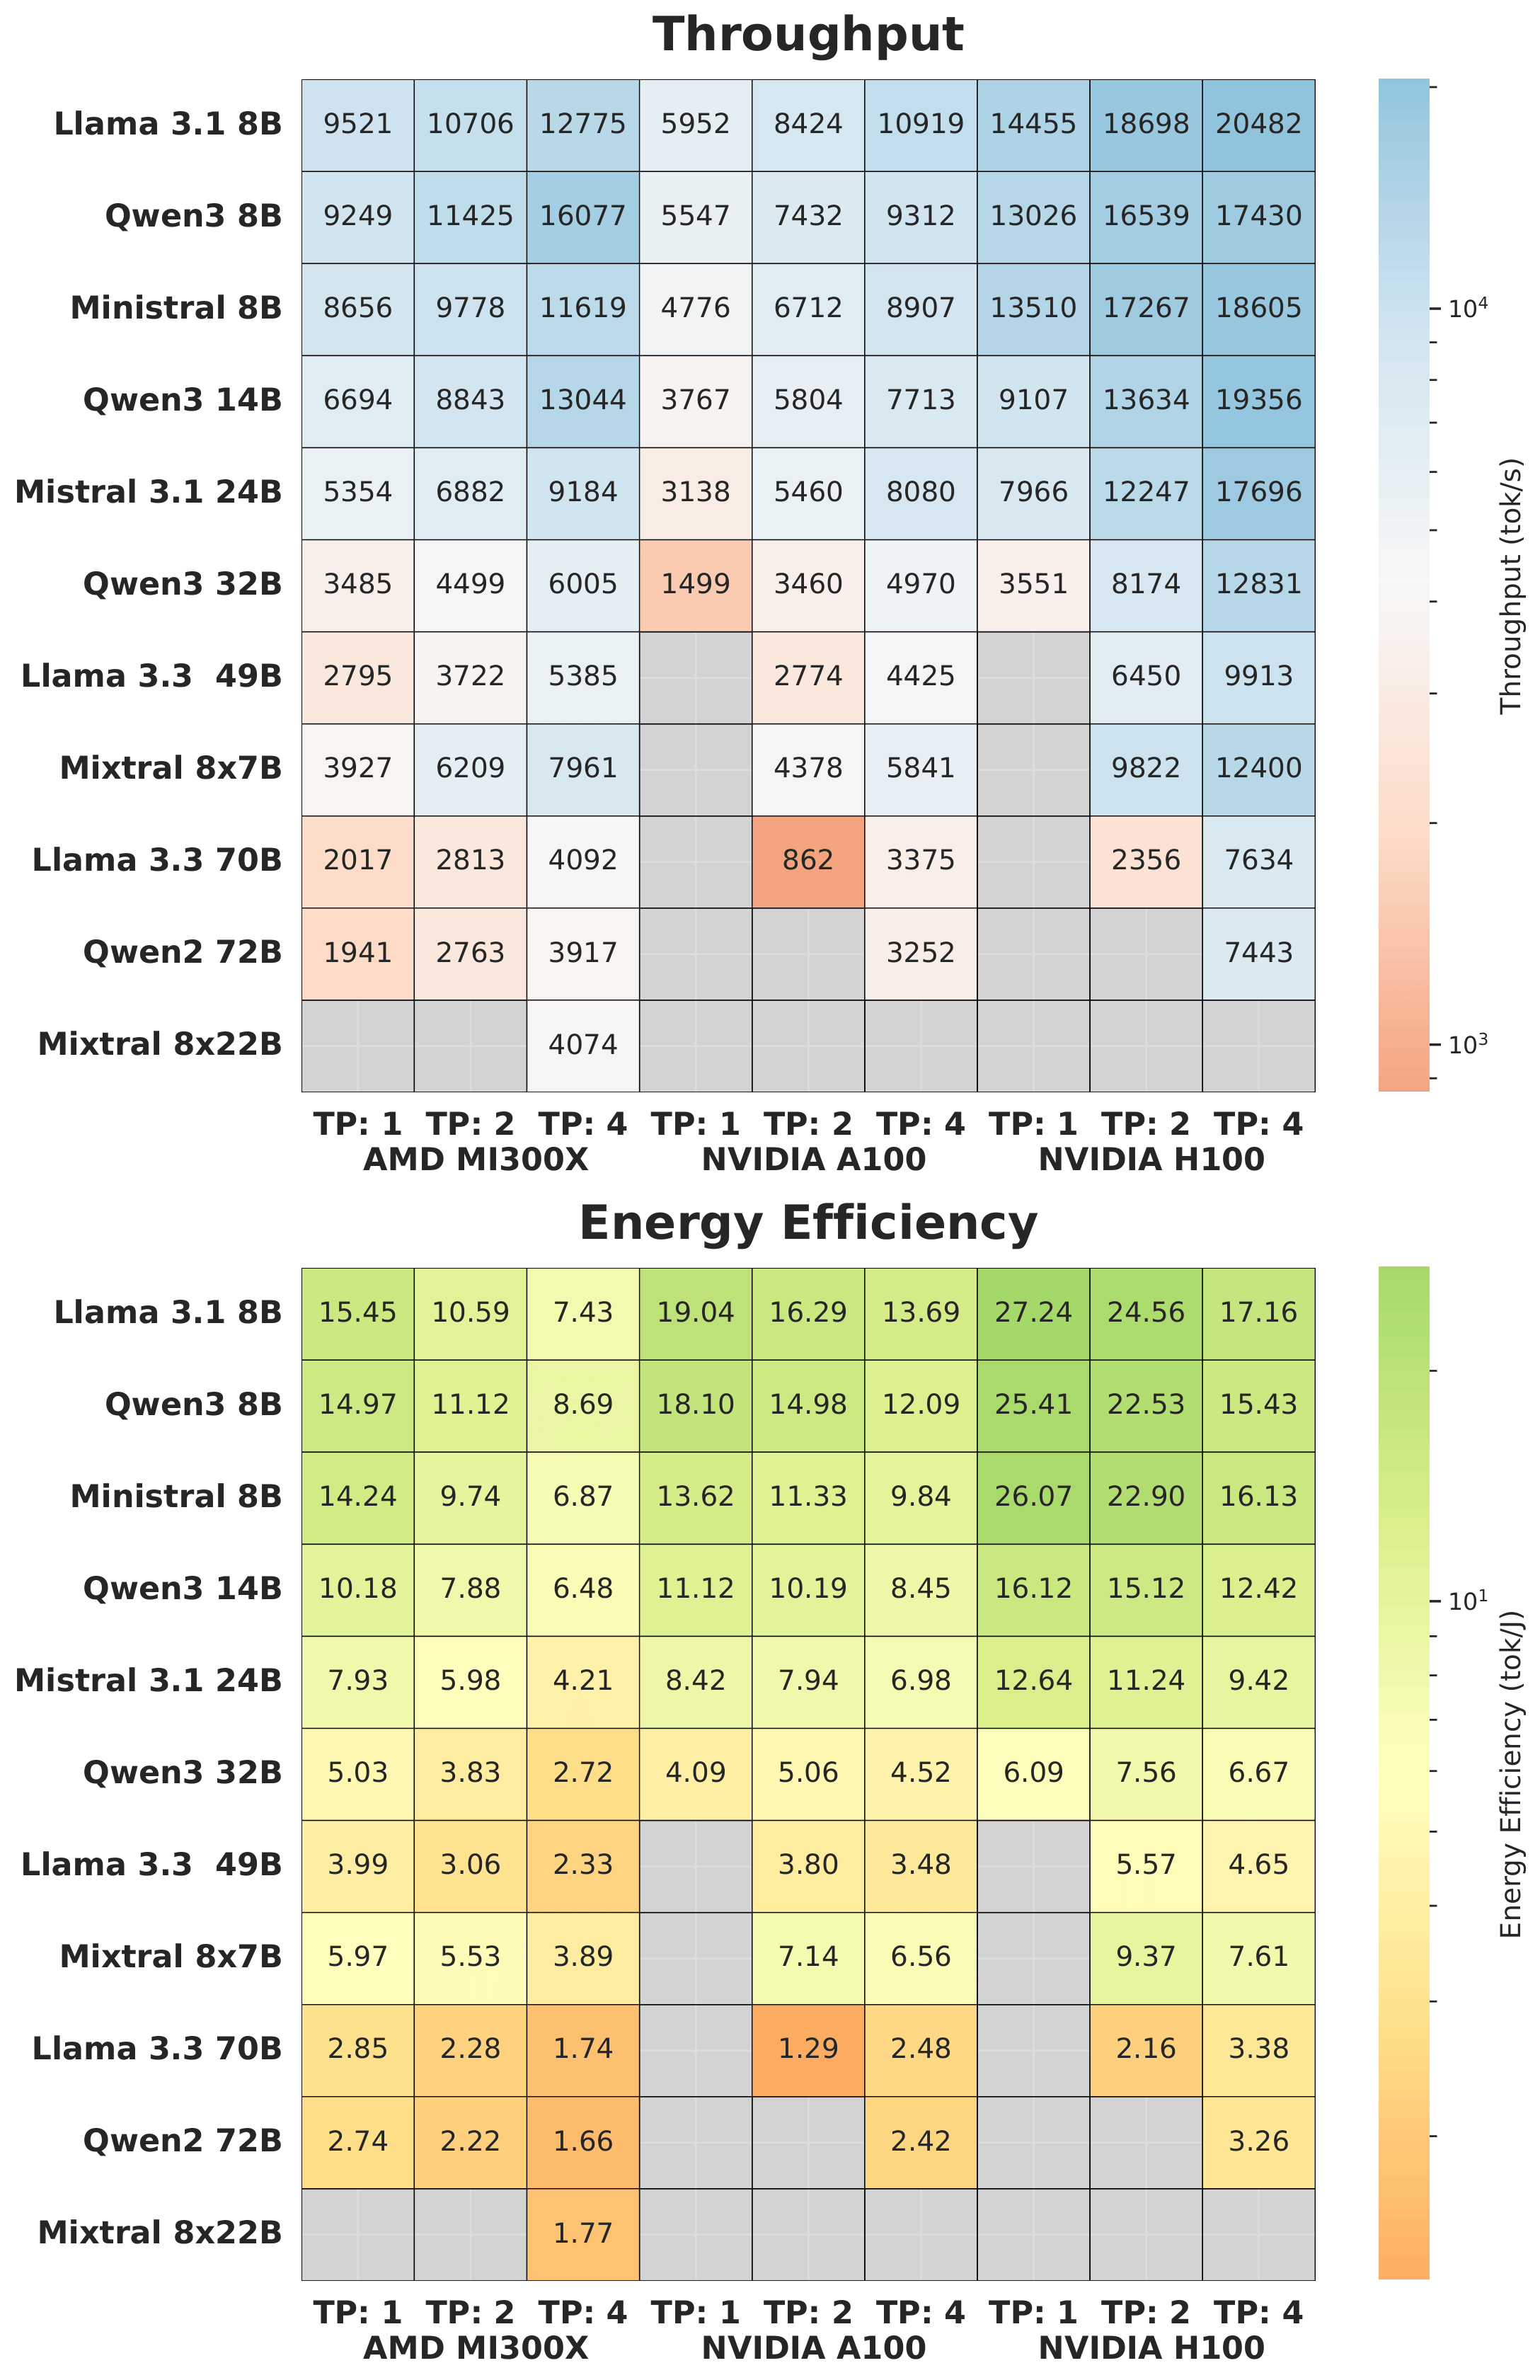
\includegraphics[width=0.9\columnwidth]{figs/heatmap Throughput (toks)_vs_Energy Efficiency (tokJ)_bfloat16.png}
    \caption{Throughput and energy efficiency heatmap across three multi-GPU nodes (bfloat16).}
    \tagpdfsetup{alttext={Throughput and energy efficiency heatmap across three multi-GPU nodes (bfloat16).}}
    \label{fig:heatmapbf16}
\end{figure}

\begin{figure}[H]
    \centering
    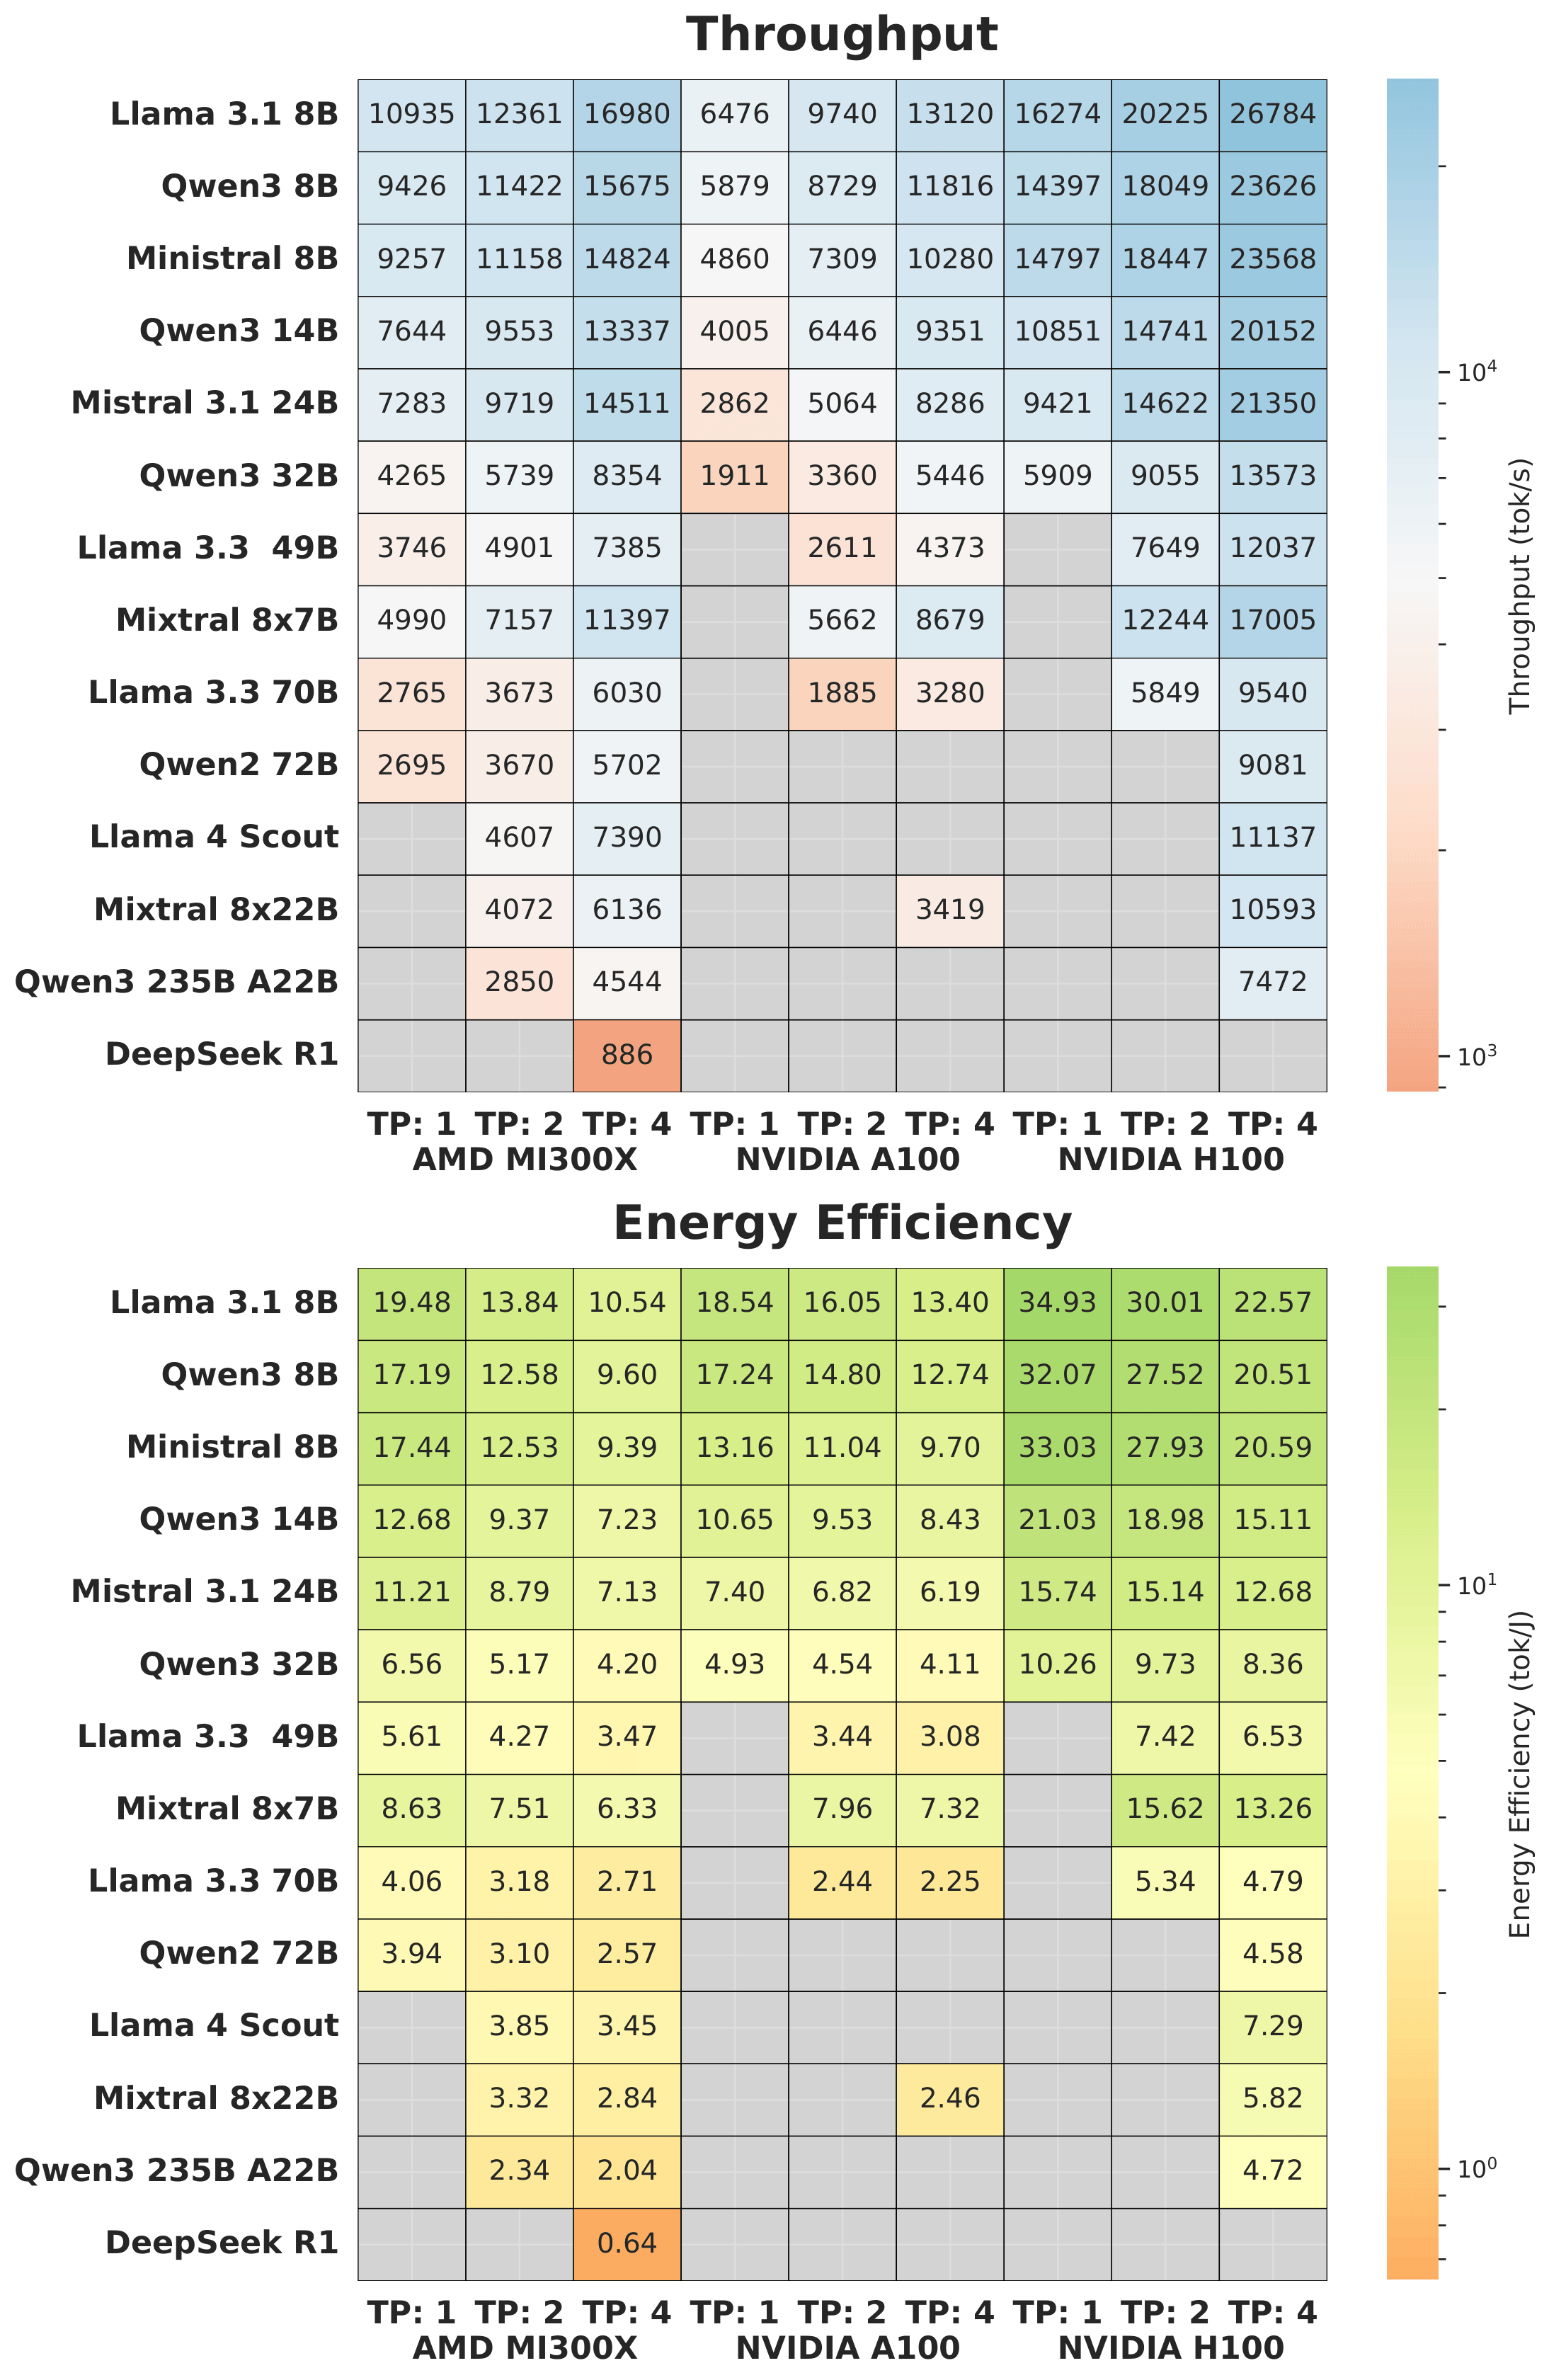
\includegraphics[width=0.9\columnwidth]{figs/heatmap Throughput (toks)_vs_Energy Efficiency (tokJ)_fp8.png}
      \caption{Throughput and energy efficiency heatmap across three multi-GPU nodes (FP8).}
      \tagpdfsetup{alttext={Throughput and energy efficiency heatmap across three multi-GPU nodes (FP8).}}
    \label{fig:heatmapfp8}
\end{figure}


\subsection{Scaling efficiency with 3D Parallelism}
Resource allocation in multi-GPU LLM inference requires balancing memory capacity and computational efficiency when choosing between Tensor and Data Parallelism. As discussed in Section \ref{chap:model:sec:multi}, Tensor Parallelism partitions model weights across GPUs, enabling larger models to run and potentially improving throughput. However, it introduces frequent all-gather operations, which result in synchronization overheads and idle GPU time.

\begin{comment}
\begin{figure}[H]
    \centering
    \includegraphics[width=0.9\columnwidth]{figs/efficiency_lineplot_Throughput per Instance_bfloat16.png}
      \caption{Throughput gain with Tensor Parallelism.}
    \label{fig:tpbars}
\end{figure}
\ref{fig:tpbars} shows how performance improves by increasing the Tensor Parallel size from 1 to 4 in three multi-GPU nodes.
\end{comment}

In our experimental results, we observe that configurations scaled purely with Data Parallelism exhibit an ideal linear scaling.
Instead, configurations that utilize a Tensor Parallel size of 2 or 4 enhance the throughput of the vLLM inference engine; however, display scaling efficiency falls short of the ideal level. Specifically, configurations with Tensor Parallel size 2 yield an average throughput improvement of approximately 33\% (29.9\% on AMD MI300X, 31.4\% on NVIDIA A100, and 37.4\% on NVIDIA H100), while those with Tensor Parallel size 4 achieve about 74\% (73.3\% on AMD MI300X, 74.5\% on NVIDIA A100, and 74.2\% on NVIDIA H100). In terms of scaling efficiency—computed as $\text{Perf}{\text{N-GPUs}} / (N \times \text{Perf}{\text{1-GPU}})$—Tensor Parallel size 2 reaches 65\% efficiency, whereas size 4 reaches 43\%. Compared to data-parallel configurations, which maintain nearly 100\% scaling efficiency, these results indicate that in offline inference scenarios, increasing the number of data-parallel instances is generally more effective for maximizing both throughput and energy efficiency than increasing tensor parallelism.

There are, however, notable exceptions to this general trend. When the model size is large enough that the weights occupy most of the available VRAM, the remaining memory becomes insufficient to support large batch sizes. In such cases, vLLM manages the limitation in two ways: it either dynamically reduces the effective batch size relative to the configured engine setting or, in the event of out-of-memory errors, performs expensive recomputations of segments of the KV matrices. As a result, models that utilize more than 80\% of GPU memory tend to achieve better performance with higher Tensor Parallelism configurations, sometimes even exceeding 100\% scaling efficiency. For instance, Qwen3 32B exhibits higher scaling efficiency with a tensor parallel size of 2 on both NVIDIA A100 and H100 nodes. Similarly, the substantial memory requirements of Llama 3.3 70B make a tensor parallel size of 4 preferable to 2 on the same hardware.

Regarding energy efficiency, a consistent pattern is evident. Data-parallel configurations demonstrate energy efficiency comparable to single-GPU setups, while configurations employing tensor parallelism tend to be less efficient. An exception again occurs for models that use more than 80\% of the available VRAM. As discussed earlier, when hardware remains constant, energy efficiency shows a strong positive correlation with throughput, with correlation coefficients ranging from 0.90 to 0.94. Therefore, optimizing throughput inherently leads to improvements in energy efficiency.

It is also noteworthy that Tensor Parallel configurations generally draw less power on average, as illustrated in \ref{fig:powbars}. However, this reduction in power consumption is insufficient to offset the performance degradation caused by inter-GPU communication overhead. In the specific cases where higher tensor parallelism yields better performance, the lower power usage contributes to energy efficiency gains that exceed the corresponding throughput improvements. This observation further highlights the importance of maintaining sufficient memory capacity for the KV cache.

\begin{figure}[h!]
    \centering
    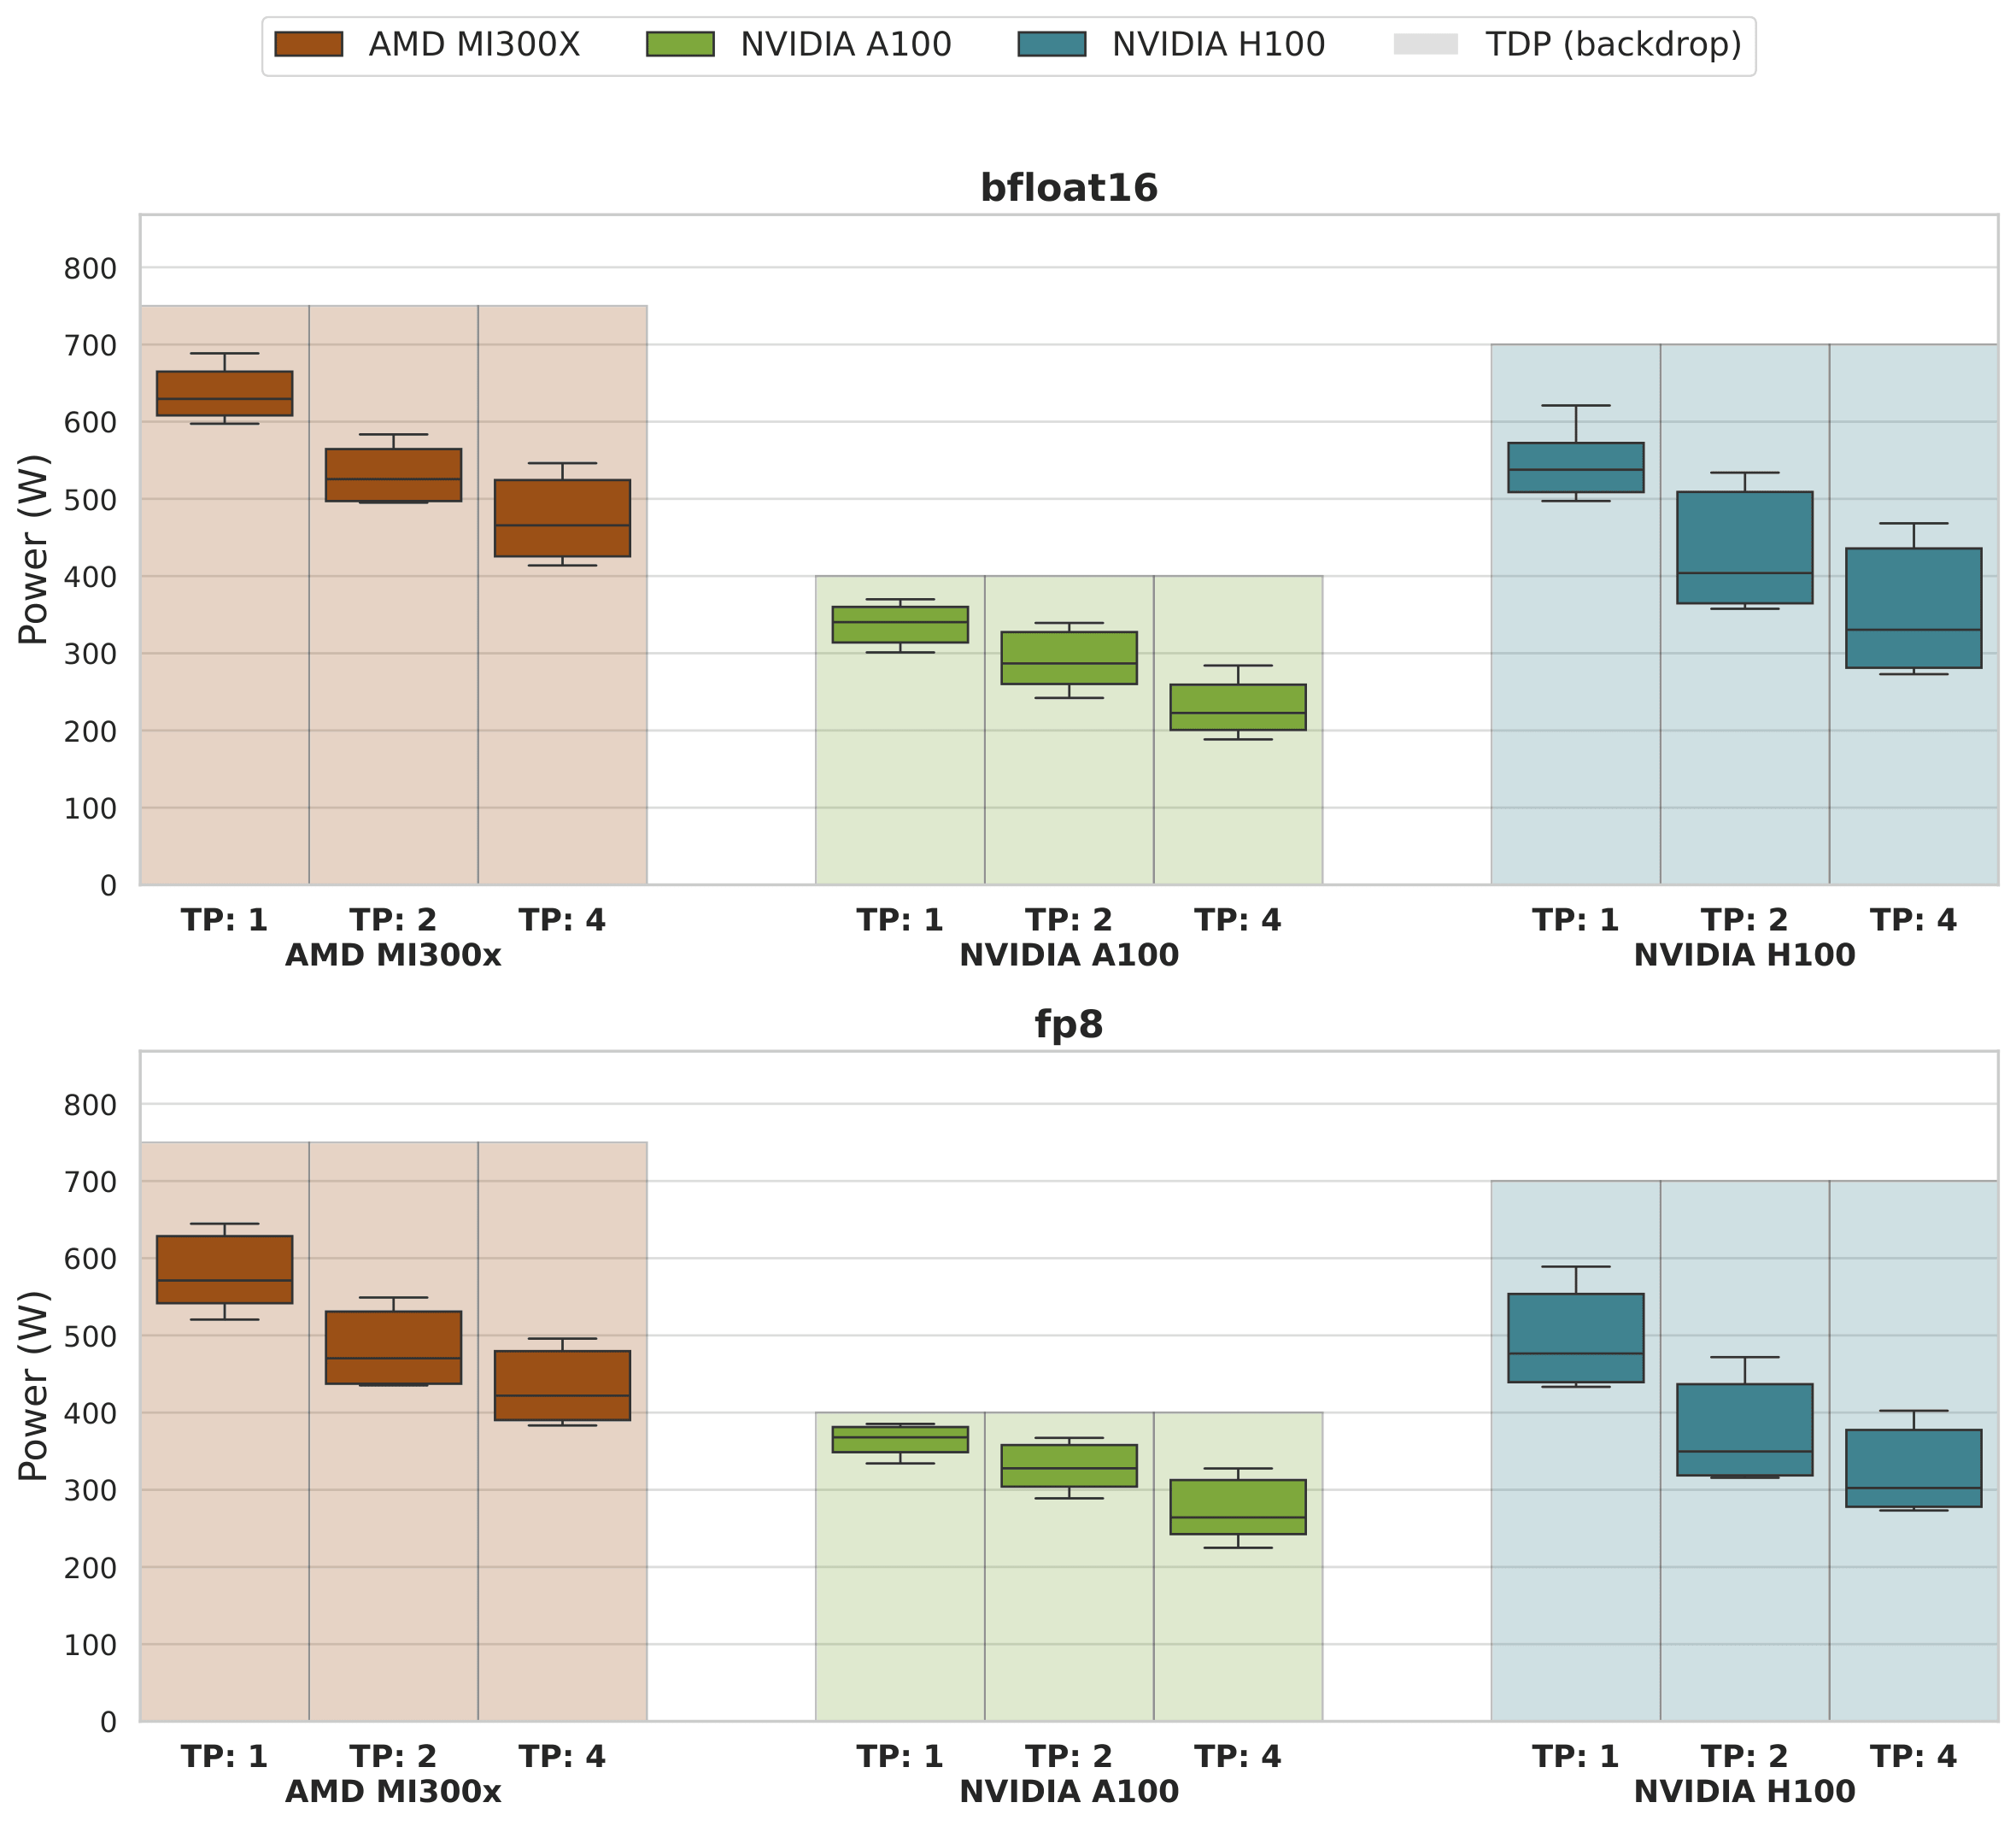
\includegraphics[width=0.95\columnwidth]{figs/efficiency_boxplot_merged_active_power_avg_bfloat16_fp8.png}
    \caption{Power consumption with Tensor Parallelism.}
    \tagpdfsetup{alttext={Power consumption with Tensor Parallelism.}}
    \label{fig:powbars}
\end{figure}

\subsection{Model Size  Scaling}
The second aspect of our analysis investigates how energy efficiency and performance evolve with increasing model size and sparsity. \ref{fig:scaling} presents the trends of four key metrics as the number of parameters increases. The trends across dense models are represented by solid lines, while dashed lines indicate the Mixture-of-Experts (MoE) model.

In Section~\ref{chap:results:sec:single}, we observe that dense models exhibit a linear increase in end-to-end latency and TTFT as model size grows, while throughput and energy efficiency decrease inversely—consistent with the behavior predicted by our performance model, consistently with what was discussed in Section \ref{chap:methods:sec:model}. This trend remains stable even when scaling to multi-GPU configurations with a fixed Tensor Parallel (TP) size.

When comparing different TP/DP configurations, we find that not all metrics scale uniformly under this weak-scaling setting. End-to-end latency and TTFT remain largely constant across TP configurations, whereas throughput and energy efficiency improve in smaller TP setups. Consequently, when considering the best attainable performance across configurations, we observe linear scaling in latency and TTFT, accompanied by an even more pronounced decline in throughput and energy efficiency as model size increases.

A distinct pattern emerges when analyzing Mixture-of-Experts (MoE) models (dashed lines in \ref{fig:scaling}). 
As discussed in \ref{chap:model:sec:moe}, Mixture-of-Experts models activate only a subset of their weights during inference, reducing the number of floating-point operations per forward pass from $2N$ to $2A$, where $N$ is the total number of parameters and $A$ is the number of active parameters. However, their memory load operations depend on the number of experts that are active at each level. In the case of a batch size of 1, loading operations also decrease from $N$ to $A$, while for larger batch sizes, most experts are loaded, resulting in a lower ideal speedup.

When observing experimental data, we can observe that, keeping constant hardware resources, MoE models consistently achieve higher performance and energy efficiency than dense models of comparable size. This demonstrates the effectiveness of the MoE architecture in scaling model parameters and accuracy while maintaining strong computational and energy efficiency. For example, Llama 4 Scout—with 109B total parameters—achieves 17\% higher throughput and 52\% better energy efficiency than the smaller Llama 3 70B on NVIDIA H100, by activating only 17B parameters during inference.
However, due to the impact of memory accesses, these gains are not strictly proportional to the degree of sparsity. On both NVIDIA H100 and AMD MI300X, Llama 4 Scout underperforms relative to Llama 3 Nemotron Super (49B), despite activating only 22B parameters.

\begin{figure}[h!]
    \centering
    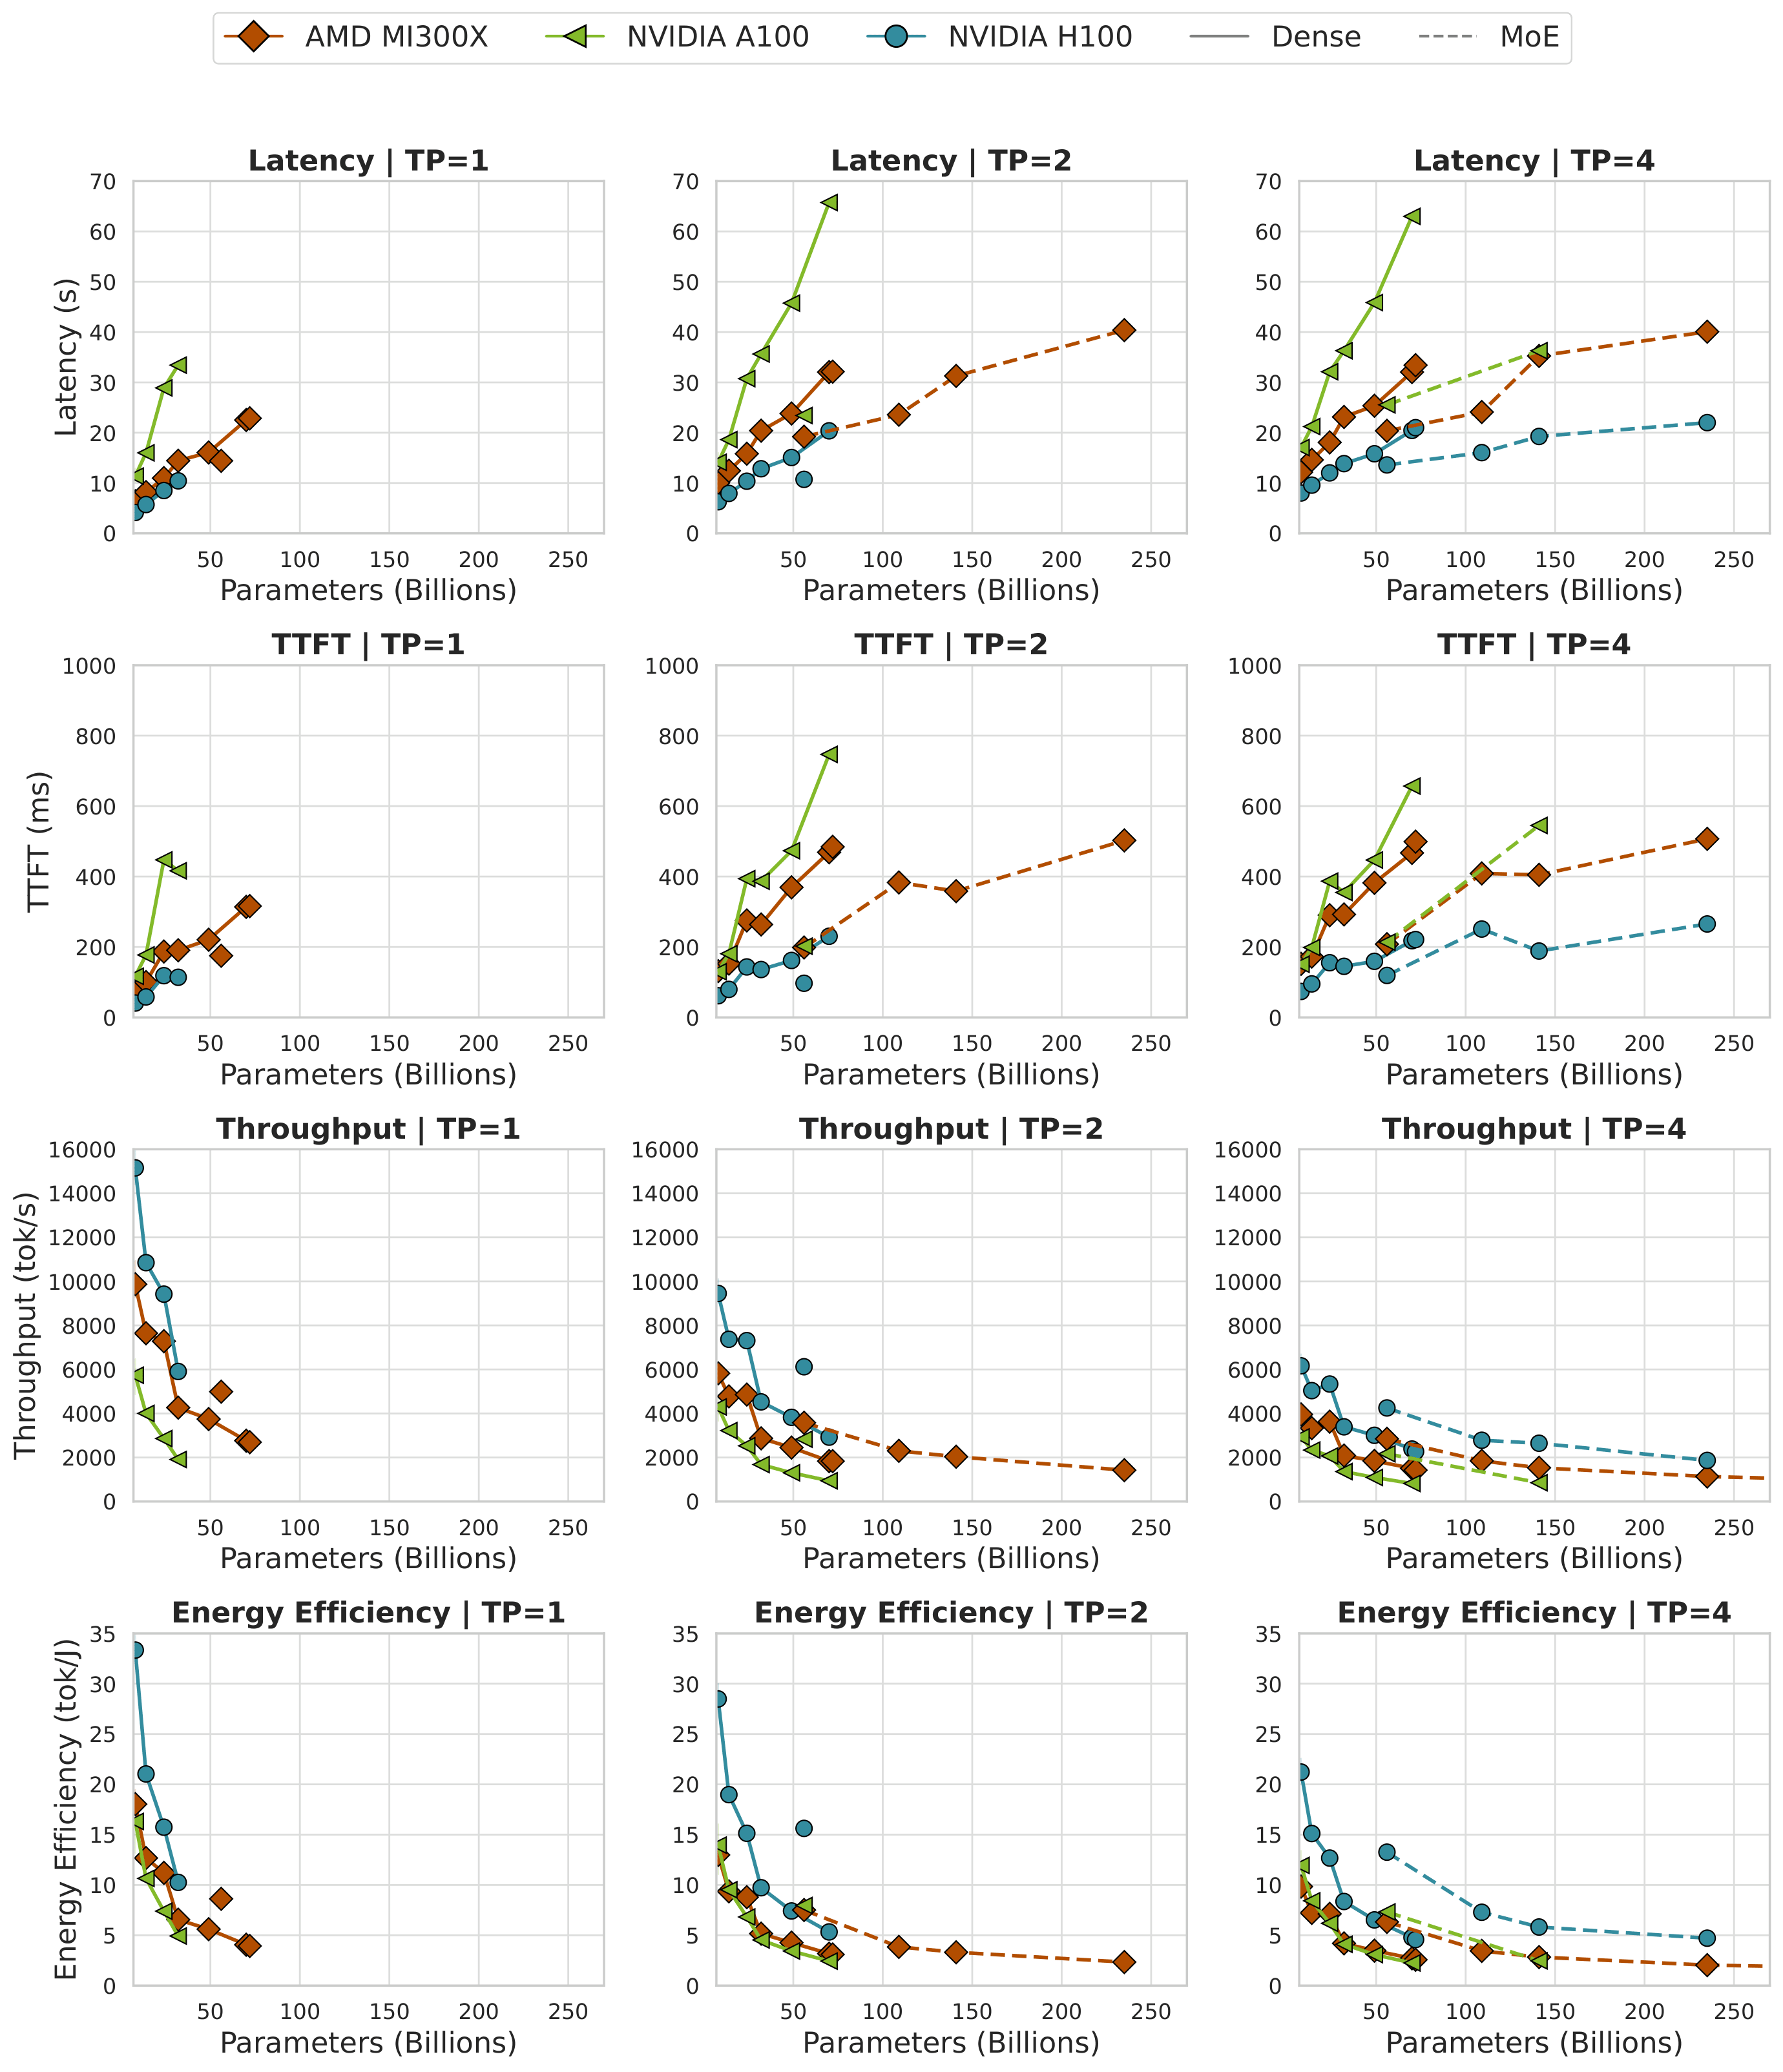
\includegraphics[width=\columnwidth]{figs/Combined_Metrics_NoBest.png}
      \caption{Scaling of performance metrics with model size.}
      \tagpdfsetup{alttext={Scaling of performance metrics with model size.}}
    \label{fig:scaling}
\end{figure}

\subsection{Tensor and Expert Parallelism}
In Section \ref{chap:background:sec:serving}, we introduced Expert Parallelism as an alternative approach to parallelizing inference in Mixture-of-Experts (MoE) models.
To evaluate its performance, we conduct a series of experiments comparing Tensor Parallelism and Expert Parallelism across four sparse large language models (LLMs). Each model is tested on both four NVIDIA H100 GPUs and four AMD MI300X GPUs, using both parallelization strategies and a range of batch sizes.

\begin{figure}[h!]
\centering
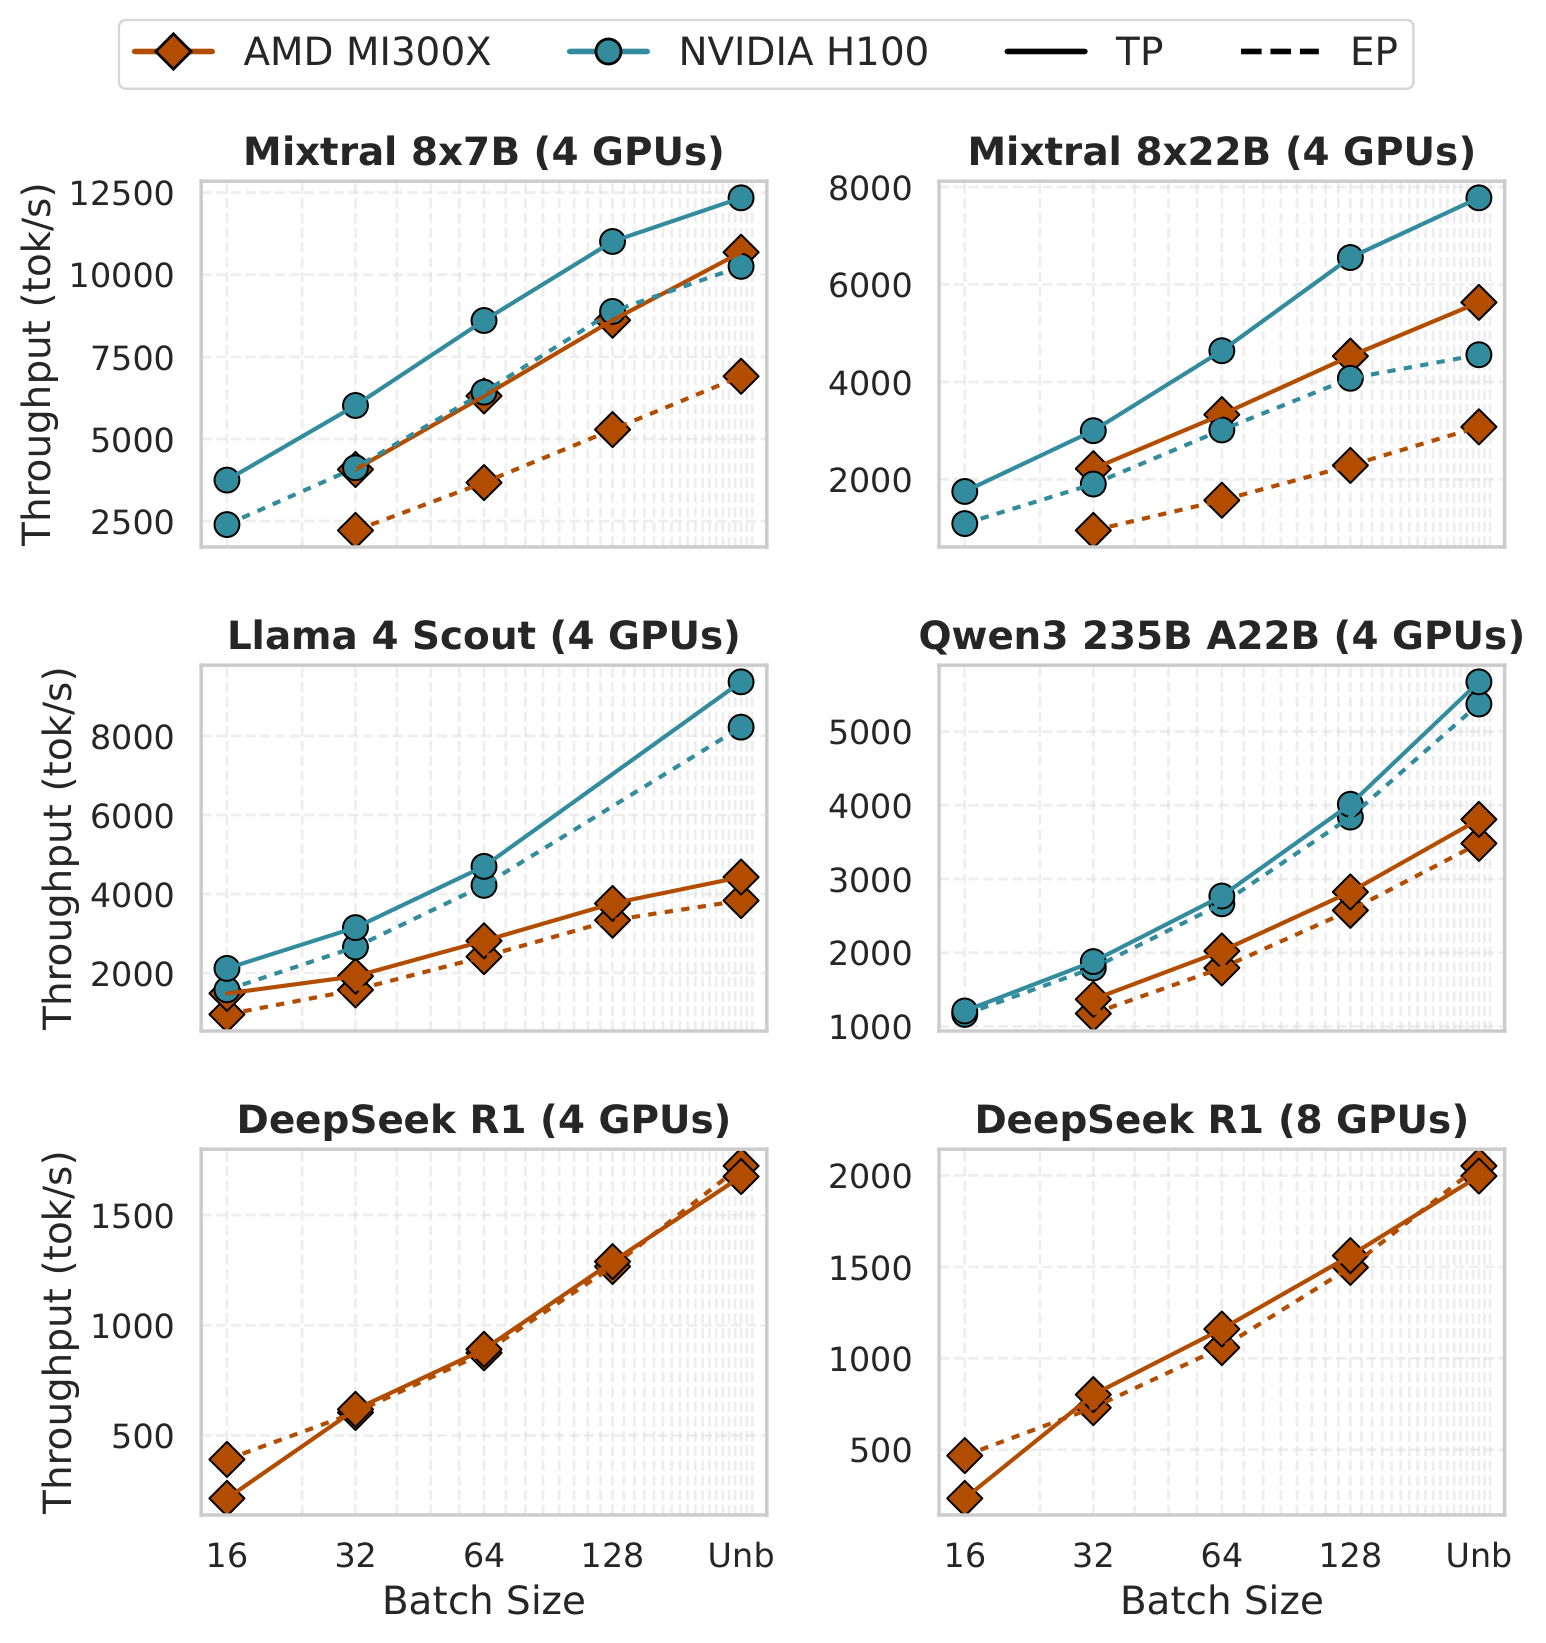
\includegraphics[width=0.75\columnwidth]{figs/combined_ep_tp.png}
\caption{Throughput using Tensor and Expert Parallelism.}
\tagpdfsetup{alttext={Throughput using Tensor and Expert Parallelism.}}
\label{fig:ep}
\end{figure}

At a first-level analysis, the results show that Tensor Parallelism consistently outperforms Expert Parallelism across all models, batch sizes, and hardware configurations—with one notable exception, which is discussed later.

A closer examination of model architectures reveals that the number of experts is a key factor driving this performance gap. Mixtral 8x22B, which employs eight experts, exhibits the largest advantage for Tensor Parallelism, achieving 61\% higher throughput on the H100 and up to 2.7 $\times$ higher throughput on the MI300X. For Llama 4 Scout (16 experts), Tensor Parallelism achieves 6\% higher throughput on the MI300X and 34\% higher throughput on the H100. Qwen3, with 128 experts, shows smaller improvements (16\% on MI300X and 4\% on H100). DeepSeek R1, however, deviates from this pattern due to its unique configuration—256 rooted experts plus one shared expert—which enables Expert Parallelism to match or exceed Tensor Parallelism at smaller batch sizes. At a batch size of 16, it achieves 82\% higher throughput with four GPUs and 100\% higher throughput with eight GPUs. As the batch size increases, this advantage diminishes, and both methods converge to similar performance levels.

The energy efficiency results largely reflect the throughput trends. Tensor Parallelism generally proves more energy-efficient, particularly for models with fewer experts. For instance, Mixtral 8x22B achieves twice the efficiency on the MI300X and a 60\% improvement on the H100, while Llama 4 Scout exhibits comparable gains. Qwen3 again shows marginal improvements (18\% on MI300X and 2\% on H100). DeepSeek R1 remains the exception: Expert Parallelism is more efficient at batch sizes of 16 or smaller, but Tensor Parallelism becomes more efficient as the batch size grows.


\subsection{GPU Model Comparison}
\ref{fig:heatmapbf16} and \ref{fig:heatmapfp8} report the throughput and energy efficiency of all the experimental results conducted with the three multi-GPU nodes in bfloat16 and FP8 precision, respectively.

Consistent with the findings presented in Section \ref{chap:results:sec:single}, the NVIDIA H100 achieves the highest throughput among all tested GPUs, in both bfloat16 and FP8 precisions. It is followed by the AMD MI300X, which consistently outperforms the NVIDIA A100. The performance gap between NVIDIA Hopper and AMD CDNA3 architectures, relative to NVIDIA Ampere, becomes more pronounced under FP8 quantization, as the newer architectures incorporate dedicated FP8 functional units that support W8A8 quantization, in contrast to W8A16 on Ampere.

In terms of energy efficiency, the results vary depending on the precision and model size. With bfloat16 precision, the NVIDIA A100 demonstrates higher efficiency than the AMD MI300X for models with fewer than 32B active parameters. However, when using FP8 quantization, the MI300X consistently exhibits superior efficiency. Across all configurations, the NVIDIA H100 maintains the highest overall efficiency at both precisions.

Memory capacity also plays a crucial role in determining performance. While both NVIDIA GPUs provide 80 GB of HBM memory, the AMD MI300X offers 192 GB, yielding two major advantages: it can accommodate larger models and requires smaller tensor parallel sizes for equivalent workloads. As discussed earlier, Tensor Parallelism introduces frequent all-gather operations that hinder performance, making lower tensor parallel sizes desirable.

When comparing performance under a fixed GPU budget (e.g., four GPUs), the MI300X often achieves higher throughput due to its larger memory capacity. This enables it to operate in pure data-parallel mode, avoiding the communication overheads inherent to high tensor parallel sizes on NVIDIA systems. For instance, with Llama 3.3 70B in bfloat16 precision, the MI300X achieves approximately 2017 tokens per second per GPU with a tensor parallel size of 1, resulting in a total throughput of 8068 tokens per second across four GPUs. In contrast, the NVIDIA H100 reaches 7634 tokens/s under the same configuration but requires a tensor parallel size of 4. A similar pattern emerges for Qwen2 72B in bfloat16 precision.

\section{Dataflow Accelerators Experiments}
\label{chap:results:sec:dsa}

Finally, we analyze LLM inference performance and energy efficiency of two state-of-the-art dataflow AI accelerators (Cerebras CS3 and Sambanova SN40L), comparing their results with NVIDIA A100 and NVIDIA H100 GPUs.
To do so, we evaluate two Llama models of different sizes: Llama 3.1 8B and Llama 3.3 70B.

For Llama 3.1 8B, Cerebras, and SambaNova provide pre-compiled artifacts that support batch sizes from 1 to 8, so we evaluate AI accelerators only within this range. In contrast, for GPUs, we test batch sizes from 1 to 128. GPU results are obtained using single-GPU inference, whereas the dataflow-accelerated systems use their full hardware configurations: one WSE for Cerebras and sixteen RDUs for SambaNova.

The larger 70B model instead is tested using 4 GPUs with Tensor parallelism on the GPU nodes and 16 RDUs on the SN40L machine. The Cerebras CS3 does not support single-node inference for this model, as its framework loads all the model weights into scratchpad memory (44 GB/WSE3), which is not capable of holding Llama 3.3 70B in bfloat16 precision (140 GB).

\subsection{Performance Comparison Across Batch Sizes}

\begin{figure}[h!]
    \centering
    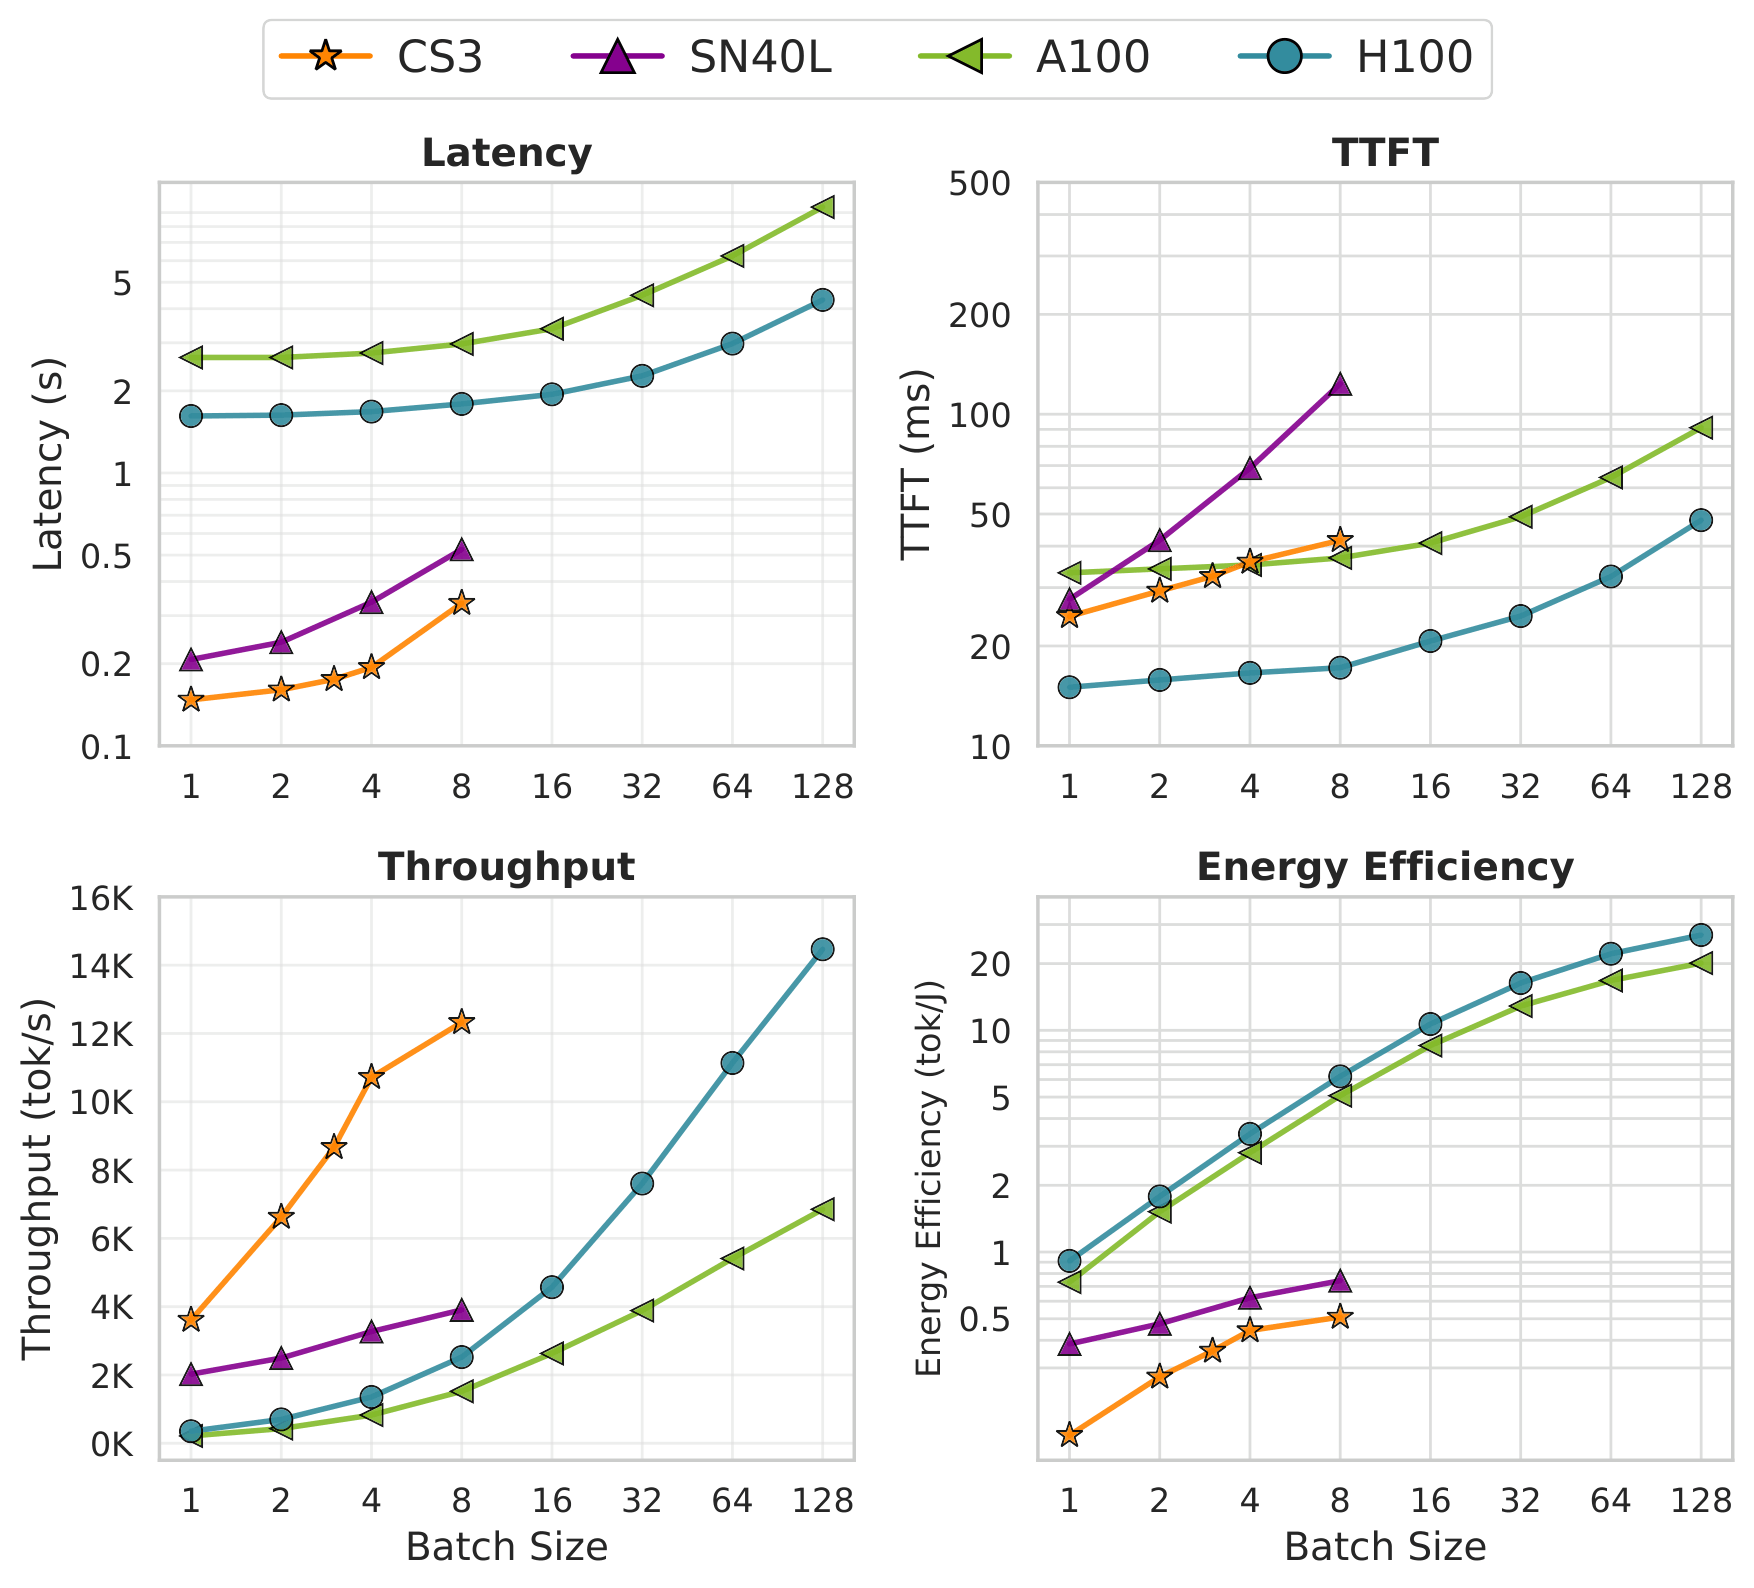
\includegraphics[width=0.8\columnwidth]{figs/testbeds_8B.png}
    \caption{Performance and energy efficiency of Llama 3.1 8B inference across AI accelerators.}
    \tagpdfsetup{alttext={Performance and energy efficiency of Llama 3.1 8B inference across AI accelerators.}}
    \label{fig:testbeds8}
\end{figure}

\ref{fig:testbeds8} and~\ref{fig:testbeds70} present the performance and energy-efficiency results for GPUs and dataflow accelerators running Llama~3.1~8B and Llama~3.3~70B, respectively, reporting four key metrics that highlight the differences in performance between GPUs and dataflow accelerators.

\begin{figure}[h!]
    \centering
    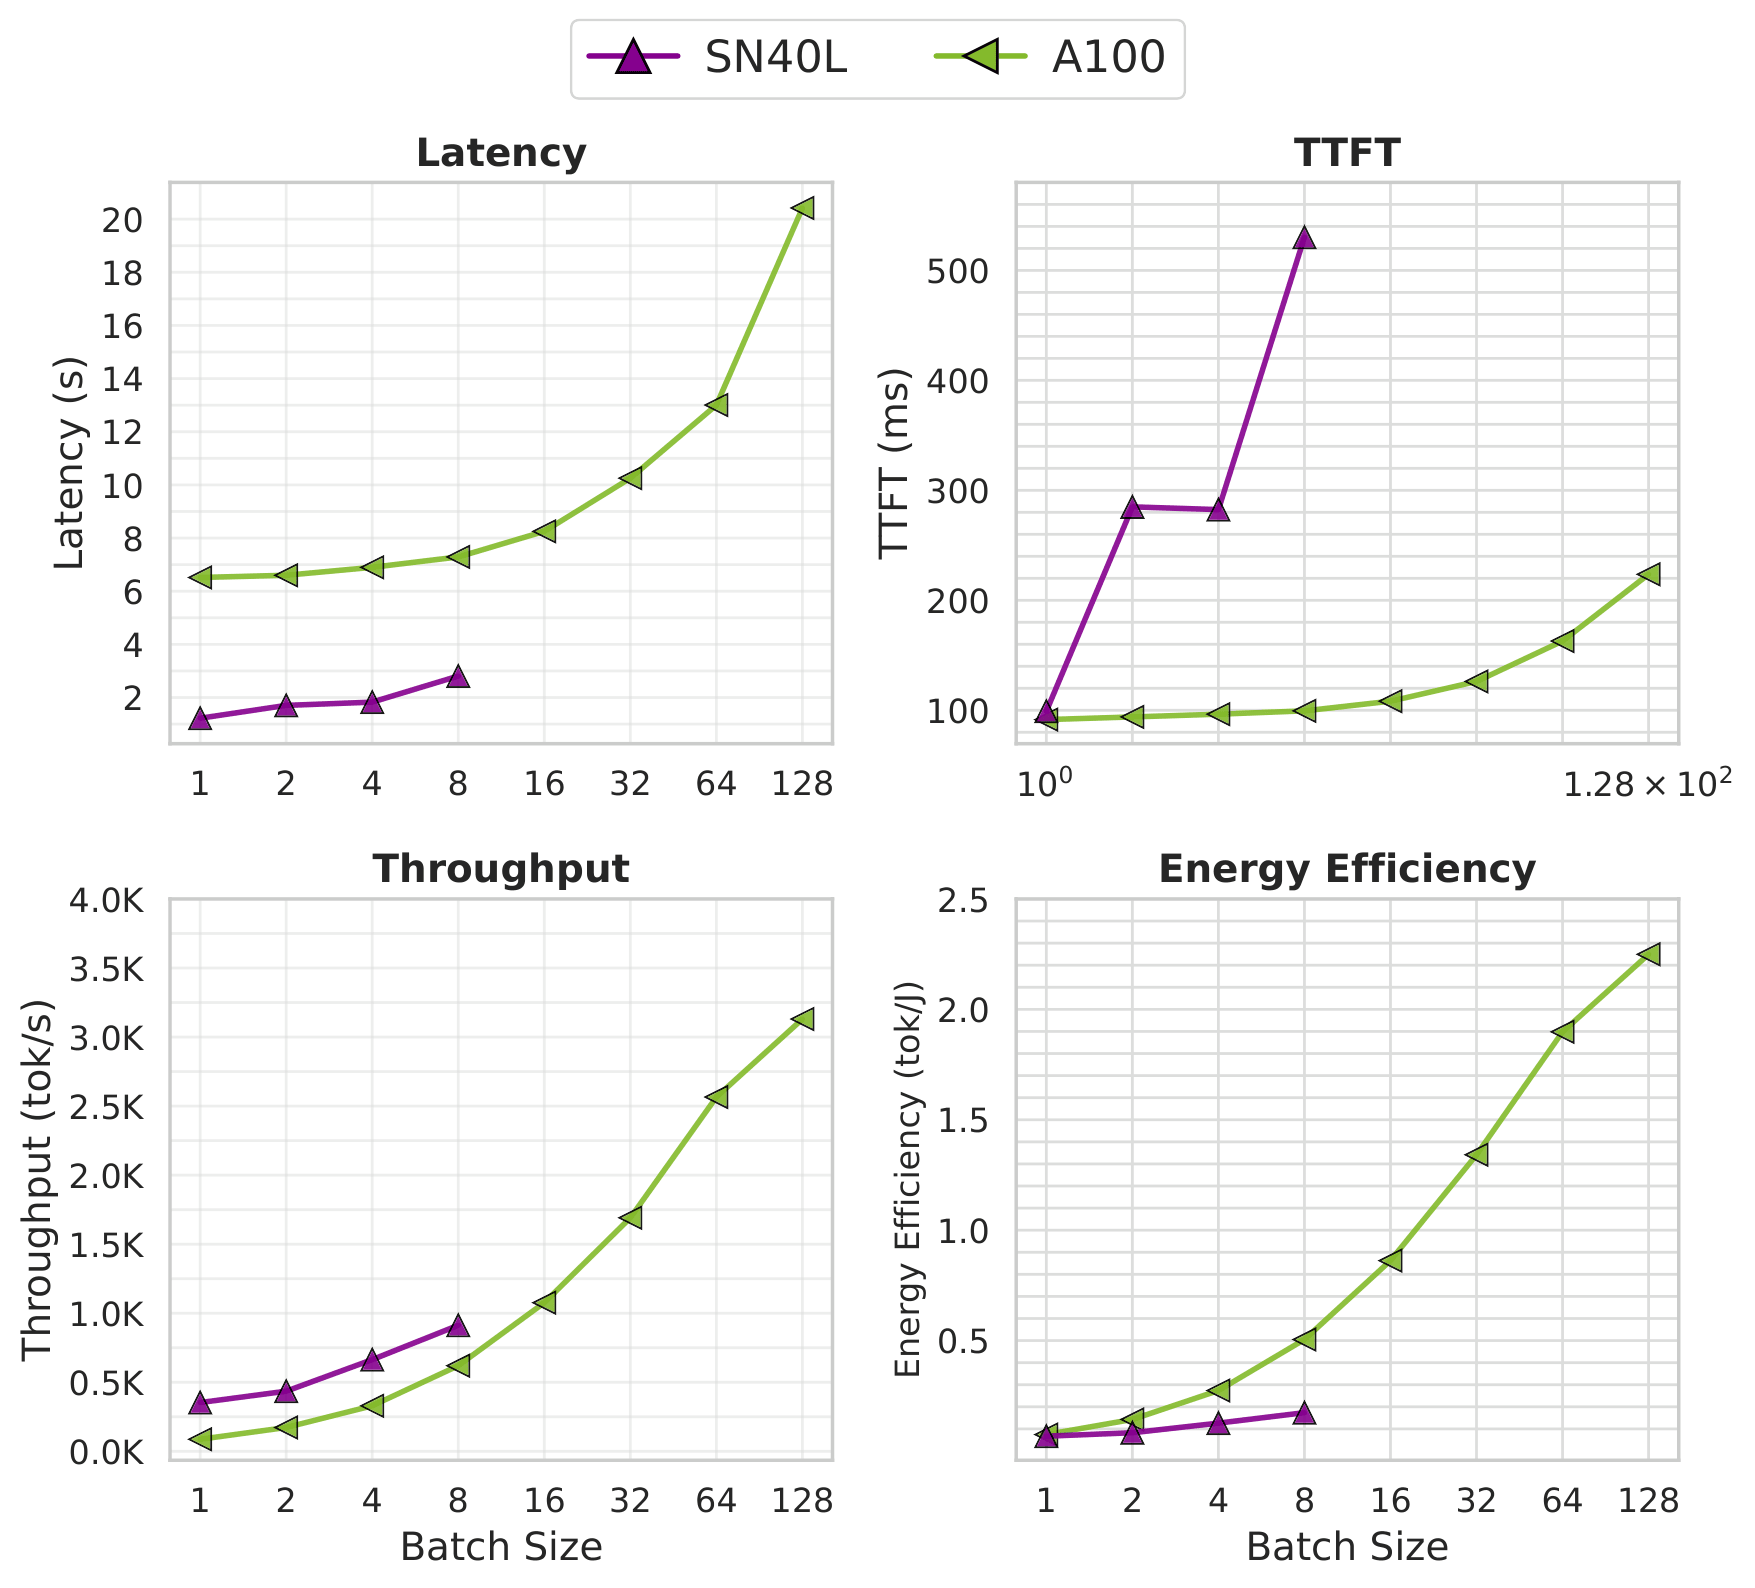
\includegraphics[width=0.8\columnwidth]{figs/testbeds_70.png}
      \caption{Performance and energy efficiency of Llama 3.3 70B inference across AI accelerators.}
    \tagpdfsetup{alttext={Performance and energy efficiency of Llama 3.3 70B inference across AI accelerators.}}
    \label{fig:testbeds70}
\end{figure}

Our experimental data clearly demonstrate how different architectures impact computation. As extensively discussed in Section \ref{chap:methods:sec:model}, LLM inference performance is directly related to the latency of the forward pass, which is composed of two parts: the latency of the computation and the latency of memory loading operations. GPUs host the model weights in off-chip HBM memories, which provide a bandwidth of approximately 1 to 5 TB/s. Dataflow accelerators, on the other hand, rely on local scratchpad memories, which are up to four orders of magnitude faster than GPUs, aiming to alleviate the impact of memory reads on the overall performance.
fi
At first, we observe that within their supported batch sizes, dataflow machines achieve markedly lower latency and substantially higher throughput than GPUs. The most pronounced improvement occurs at batch size 1, where the computation is the most memory-bound.
NVIDIA A100 reaches 215 tokens/s, compared to 3609 tokens/s (16.8$\times$) on the Cerebras CS3 and 2024 tokens/s (9.41$\times$) on the SambaNova SN40L.
The SamabaNova SN40L also outpaces GPUs with Llama 3.3 70B, achieving 353 tokens/s at a batch size of 1, compared to 88 tokens/s (4.01$\times$) obtained with 4 NVIDIA A100s working with Tensor Parallelism.

Increasing the batch size also increases the operational intensity $OI$, allowing GPUs to progressively close the GAP. In their supported batch size range (1-8), dataflow accelerators still outpace GPUs in terms of latency and throughput. However, due to the larger impact of computation on overall latency, we notice that dataflow accelerators display notably steeper increases in end-to-end latency and TTFT compared to those of GPUs.

Another observation regards peak throughput.
We established that dataflow machines exhibit superior performance at small batch sizes, but we also assessed the fact that their maximum supported batch size is substantially lower, sometimes due to a lack of compile artifacts for larger batch size configurations. In fact, both Cerebras and SambaNova provide precompiled artifacts that allow running at fixed batch sizes of 1 to 8. vLLM, on the other hand, handles batch sizes dynamically, allowing us to test batch sizes up to 128.
In an offline scenario, where the maximum achievable throughput using the optimal batch size is the only relevant performance metric, we observe that the capacity of GPUs to scale to larger batch sizes allows them to narrow the performance gap in terms of peak throughput. Cerebras, at a batch size of 8, produces 12327 tokens/s, outperforming both the NVIDIA A100 and the AMD MI300x. However, it is still outperformed by the NVIDIA H100 at a batch size of 128, which achieves 14,455 tokens/s. The SambaNova SN40L instead peaks at 3,907 tokens/s with a batch size of 8.
From this, we can conclude that the performance benefits of modern dataflow accelerators are noticeable, particularly in online settings with low batch sizes and a limited number of requests per node. In offline batch-inference jobs, the dynamic batch size supported by GPUs makes this architecture still preferred.

This causes dataflow accelerators to dominate online inference scenarios with a reduced number of concurrent requests, while in an online scenario where the only requirement is high throughput, they lose their competitive advantage in terms of raw performance.

\subsection{Comparison of ITL and TTFT}

\begin{figure}[h!]
    \centering
    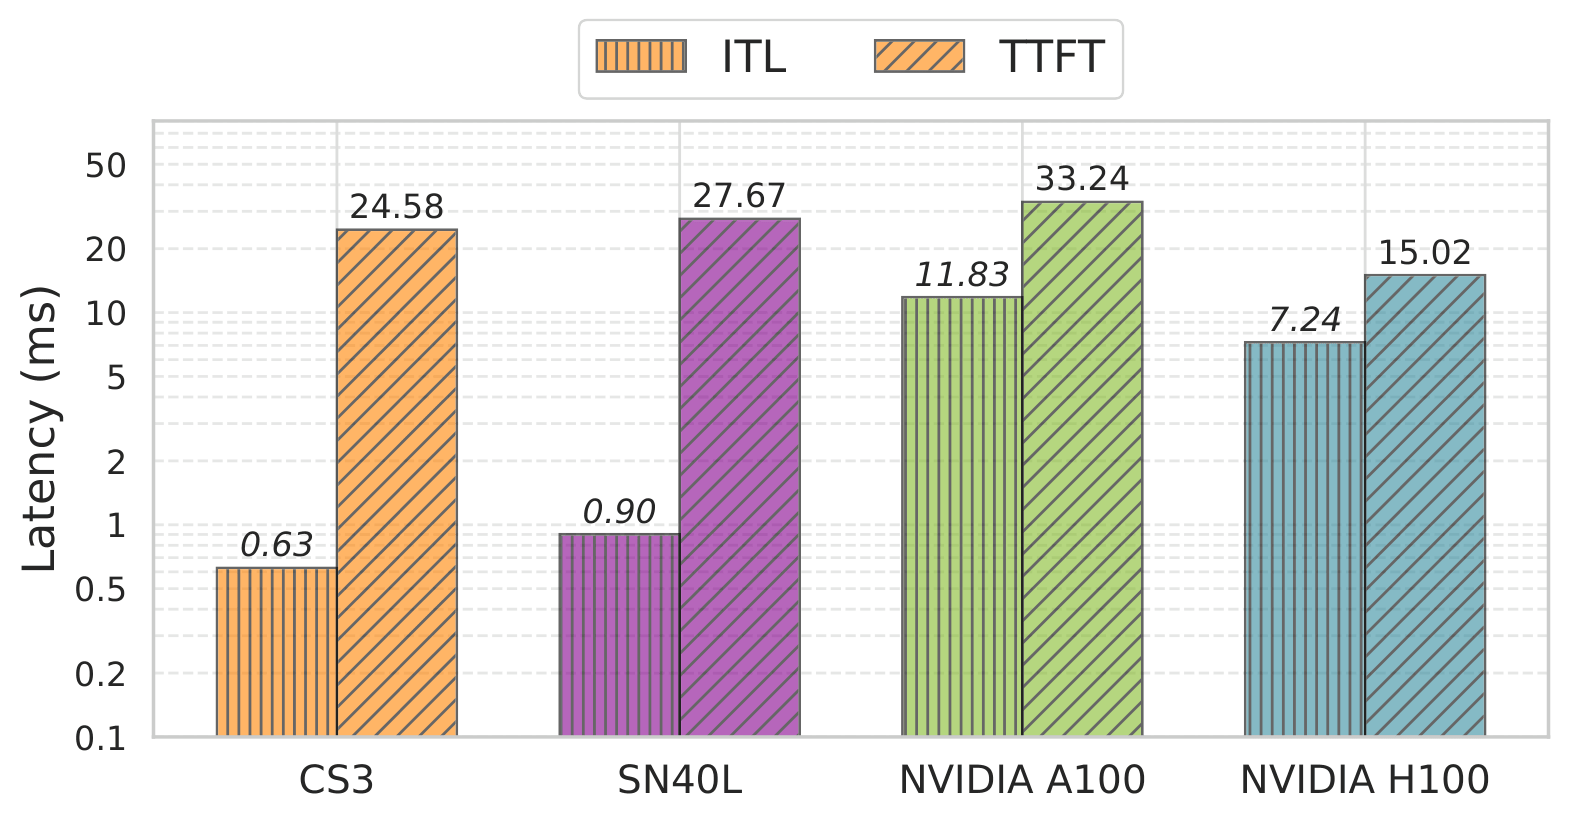
\includegraphics[width=\columnwidth]{figs/itl_ttft.png}
      \caption{Time-to-first-token (TTFT) and Inter Token Latency (ITL) of GPUs and dataflow accelerators.}
      \tagpdfsetup{alttext={Time-to-first-token (TTFT) and Inter Token Latency (ITL) of GPUs and dataflow accelerators.}}
    \label{fig:itl-ttft}
\end{figure}

Digging further into the impact of memory bandwidth on computation, we compare the ITL and TTFT across the different architectures. As discussed in \ref{chap:methods:sec:metrics}, TTFT is the average latency of the compute-bound prefill phase, while ITL indicates the average latency of the memory-bound decode phase.
\ref{fig:itl-ttft} displays TTFT and ITL of Llama 3.1 8B at batch size 1.
It allows us to observe once again how the benefit of dataflow accelerators stems from their improved data locality and memory bandwidth. In fact, while the TTFT of the SambaNova SN40L and the Cerebras CS3 is comparable with that of NVIDIA GPUs, the ITL is faster by one order of magnitude. Precisely, the Cerebras CS3 achieves an 18.8 $\times$ lower ITL compared to the NVIDIA A100, while SambaNova shows a 13.1 $\times$ improvement. A similar pattern appears when comparing Llama 3.3 70B performance: the SambaNova SN40L achieves slower TTFT compared to 4 NVIDIA A100 (99 ms compared to 91 ms), while having a 5.18 $\times$ shorter ITL (5.6 ms compared to 29 ms).

\subsection{Energy Efficiency}
\begin{figure}[H]
    \centering
    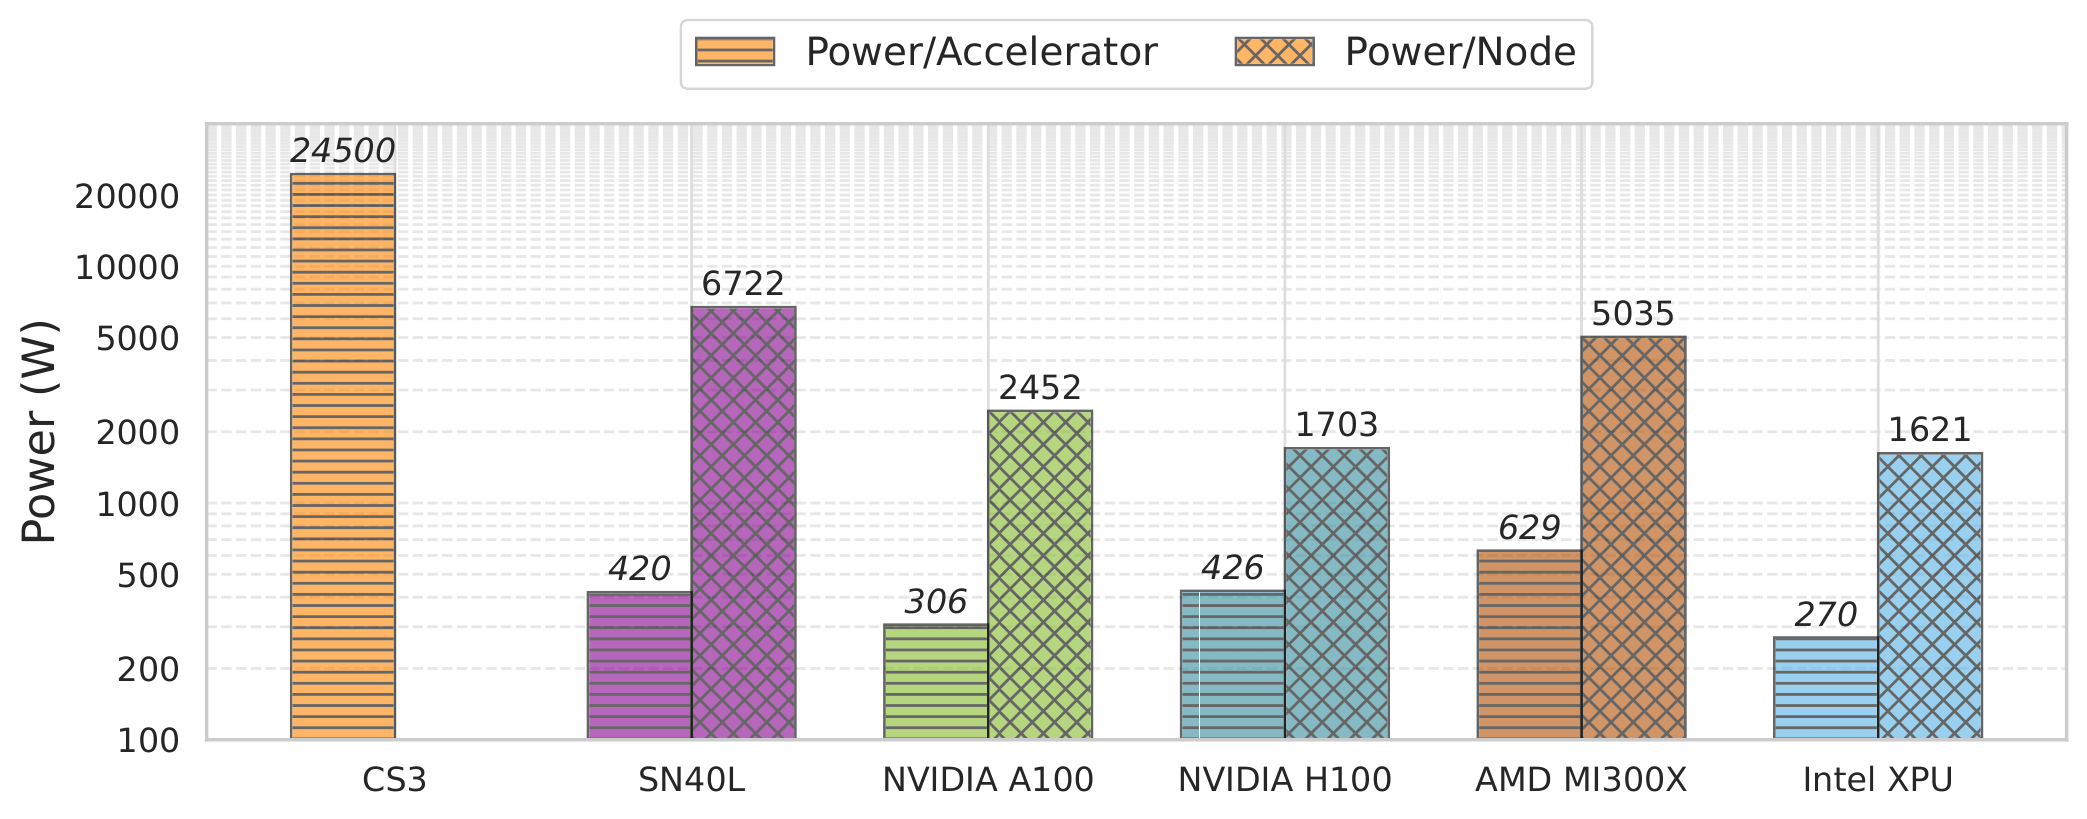
\includegraphics[width=\columnwidth]{figs/power_testbeds.png}
      \caption{Power consumption of GPUs and AI accelerators.}
      \tagpdfsetup{alttext={Power consumption of GPUs and AI accelerators.}}
    \label{fig:power}
\end{figure}

Finally, we analyze energy efficiency. To benefit from reduced memory bandwidth, dataflow accelerators employ a substantially larger number of cores that store weights and activations in their local memory, resulting in higher overall power consumption. As shown in \ref{fig:power}, to run Llama 3.1 8B in half precision, Cerebras CS3 draws around 24500W of power, and the SambaNova SN40L uses 420W per RDU, for a total of 6722W for the whole SN40L-16R system. Compared to the multi-GPU nodes, we observe that for the same model at a batch size of 16, GPUs use between 306 W and 630W of power.

For this reason, at no batch size, dataflow accelerators exhibit competitive energy consumption compared to GPUs (as shown in \ref{fig:testbeds8} and \ref{fig:testbeds70}), even though they display substantially better performance.

For this reason, we can conclude that a trade-off exists between low-latency, throughput, and energy efficiency among different types of accelerators.

\chapter{Related Work}
\label{chap:related}

As large language model (LLM) inference becomes an increasingly significant contributor to datacenter energy consumption, research on performance and energy efficiency has grown substantially. This section surveys the most relevant work across GPU-based LLM inference, Mixture-of-Experts (MoE) model evaluation, and dataflow accelerator performance.

\section{LLM Inference on GPUs}

Chitty-Venkata et al. ~\cite{LLMInfbench} provides one of the most comprehensive evaluations of modern LLM inference and serves as the primary point of reference for this thesis. The benchmark examines several major dimensions of inference performance.

First, it evaluates a broad set of model architectures, covering both dense and Mixture-of-Experts models from the LLaMA, Mistral, and Qwen families. The comparison spans two parameter scales: 7B models (LLaMA-2-7B, LLaMA-3-8B, Mistral-7B, Qwen-2-7B) and 70B–72B models (LLaMA-2-70B, LLaMA-3-70B, Mixtral-8x7B, Qwen-2-72B).

Second, the study analyzes token-generation parameters, including input length, output length, and batch size, assessing how these factors affect both latency and throughput.

Third, it compares performance across multiple hardware platforms, including NVIDIA A100, H100, and GH200 GPUs, as well as SambaNova SN40L and Habana Gaudi2 dataflow accelerators.

Fourth, it measures performance across different inference frameworks, such as vLLM, DeepSpeed-MII, llama.cpp, and TRT-LLM, enabling a cross-stack comparison.

Finally, the benchmark studies the effect of several optimization techniques, including KV caching, quantization, and other runtime-level optimizations.

Performance is characterized using key metrics: time to first token (TTFT), inter-token latency (ITL), throughput (input and output tokens multiplied by batch size per unit latency), and performance per watt based on average power consumption.

Building upon this work, our study places a stronger emphasis on energy efficiency and multi-GPU scaling behavior, while also extending the evaluation to dataflow accelerators.

A complementary study from the same authors ~\cite{chitty2025moe} analyzes the performance of several Mixture-of-Experts LLMs and vision–language models (VLMs), focusing on the architectural factors that shape their inference characteristics.


\section{Energy Efficiency of LLM Inference}

Several works focus specifically on the energy usage of LLM inference on modern GPUs.  

Fernandez et al.~\cite{fernandez2025energy} examine the impact of optimizations such as continuous batching, kernel compilation, and PagedAttention.  

Wilhelm et al.~\cite{wilhelm2025beyond} analyze test-time compute strategies—including majority voting and Chain-of-Thought prompting—exploring the efficiency–accuracy trade-off.  

Wilkins et al.~\cite{wilkins2024offline} characterize energy and performance across seven LLMs running on NVIDIA A100 GPUs.  

Dynamo-LLM~\cite{stojkovic2025dynamollm} benchmarks six models on H100 GPUs under varied tensor-parallel configurations, with a focus on multi-GPU scaling efficiency.  

Other works investigate GPU frequency scaling as a mechanism to improve the performance–efficiency balance~\cite{maliakel2025investigating, kakolyris2024slo, stojkovic2024towards}.

Unlike these studies, our analysis jointly evaluates performance and energy efficiency across modern GPUs from multiple vendors (NVIDIA, AMD, and Intel), as well as across three dataflow AI accelerators, yielding new insights into LLM inference across diverse deployment environments.

\section{Dataflow Accelerators}

Several studies have examined the performance of dataflow accelerators.  
Emani et al.\ published two influential works~\cite{Emani2021, Emani2022}.  
The first compares emerging AI accelerators—including the SambaNova SN10-8R, Cerebras CS-2, Graphcore IPU M-2000, and GroqNode—against the NVIDIA A100 GPU. The workloads include deep learning primitives, MLPerf benchmark models (ResNet, U-Net, BERT), and scientific machine learning applications. This initial study characterizes execution time and computational throughput but does not measure power consumption.

The second study evaluates LLM inference and training performance across five dataflow accelerators, comparing them against NVIDIA A100 and AMD MI250 GPUs using two LLMs (GPT-2 XL and GenSLM).

Ferdaus et al.~\cite{ferdaus2025evaluating} further examine BERT training and inference performance, as well as energy efficiency, on four dataflow accelerators, again comparing the results with those of the NVIDIA A100.  

While these studies form the foundation of our analysis, they primarily evaluate older LLMs that no longer reflect the current state of the art. Our work, therefore, updates and extends this line of research using modern LLM architectures and contemporary accelerator platforms.

\section{MLPerf}

MLPerf is the most widely used benchmark suite for evaluating the performance of systems on machine learning workloads. Introduced in 2018 by the MLCommons organization—a consortium formed by industry and academic partners—it provides standardized, open, and reproducible methodologies for comparing hardware and software platforms. The suite comprises three major components: MLPerf Training, MLPerf Inference, and MLPerf Power.

MLPerf Training~\cite{mattson2020mlperf} focuses on end-to-end training performance, reporting the time required for a system to train a model to a specified target accuracy. The workloads correspond to the same models used in the Inference benchmark, enabling consistent cross-comparisons between training and inference performance.

MLPerf Inference~\cite{reddi2020mlperf} evaluates the performance of systems running pre-trained machine learning models across tasks such as image classification, object detection, natural language processing, and recommendation. It measures both latency and throughput across a variety of deployment scenarios, including datacenter, edge, and mobile environments. To capture real-world usage conditions, MLPerf Inference defines four load-generator scenarios. The single-stream scenario processes a single request stream with batch size one, emphasizing strict latency constraints. The multi-stream scenario also uses a single stream but with a fixed arrival pattern and batch sizes greater than one. The server scenario models unpredictable request arrivals across multiple streams while maintaining batch size one. Finally, the offline scenario captures throughput-oriented batch processing where all inputs are available in advance, and latency is not a limiting factor.

For language workloads—those most relevant to our study—the current MLPerf Inference benchmark includes six LLMs: BERT-Large, GPT-J, Llama2-70B, Llama3-405B, Mixtral-8x7B, and DeepSeekR1. These models span parameter sizes from 340M to 670B and include both dense and Mixture-of-Experts architectures, enabling comparisons that reflect contemporary large-scale LLM deployments.

MLPerf Power~\cite{Tschand2024} provides the standardized methodology for measuring energy consumption during MLPerf Training and Inference workloads. The guidelines emphasize that commonly used metrics such as Thermal Design Power (TDP) and Power Supply Unit (PSU) ratings do not accurately represent real system-level power usage, as they incorporate significant safety margins and fail to capture dynamic fluctuations in power draw. MLPerf Power, therefore, offers more precise measurement requirements to support reliable assessments of energy efficiency across diverse hardware platforms.
\chapter{Conclusion}
\label{chap:conclusion}


In this thesis, we make the following contributions:

\begin{itemize}
    \item We present, in Chapter~\ref{chap:hardware}, a detailed survey of contemporary LLM inference accelerators and analyze the architectural challenges that shape modern hardware design for large-scale inference.

    \item We develop a performance benchmark that systematically evaluates the main determinants of LLM inference performance, including model size and sparsity, batch size, quantization strategies, and multi-GPU execution techniques.

    \item We conduct a comprehensive evaluation of a diverse set of accelerators, including six GPUs and two dataflow systems. For all platforms, we measure both performance and energy efficiency, addressing an important gap in prior work, which has predominantly focused on performance alone.

    \item We provide a principled analysis of dataflow accelerator behavior in LLM inference, clarifying how batch size influences throughput, latency, and energy efficiency, and dispelling common misconceptions regarding their performance characteristics.
\end{itemize}

Our evaluation yields several important conclusions regarding the joint performance–energy efficiency trade-offs across accelerator families. Dataflow accelerators deliver substantially higher efficiency—often an order of magnitude better than GPUs—at the small batch sizes ($\le 8$) that dominate online, latency-sensitive inference. GPUs, however, excel in high-throughput offline inference due to their larger HBM capacity, mature software ecosystems, and support for FP8 execution, which collectively enable aggressive optimizations that compensate for their lower low-batch efficiency. Taken together, these results highlight the complementary strengths of GPUs and dataflow accelerators, clarifying which architectures are best suited for different LLM deployment scenarios.


% =====================================
% Back Matter
% =====================================

\backmatter

\singlespacing

\iflatexml
  \IfFileExists{thesis.bbl}{% =====================================
% Accessible PDF Setup (Overleaf Safe)
% =====================================

\ifdefined\DocumentMetadata
  \DocumentMetadata{
    lang=en-US
  }
\fi

\documentclass[12pt,reqno,oneside]{amsbook}

% =====================================
% Encoding (required for screen readers)
% =====================================

\usepackage[T1]{fontenc}
\usepackage[utf8]{inputenc}

\ifdefined\pdfglyphtounicode
  \input{glyphtounicode}
  \pdfgentounicode=1
\fi

% =====================================
% Language
% =====================================

\usepackage[english]{babel}
\usepackage{latexml}

% =====================================
% Math
% =====================================

\usepackage{amsmath,amssymb,amsthm}

% =====================================
% Graphics
% =====================================

\usepackage{graphicx}
\usepackage{subcaption}

% =====================================
% Code
% =====================================

\iflatexml
\else
  \usepackage{listings}
\fi
\usepackage{comment}

% =====================================
% Layout
% =====================================

\usepackage{geometry}
\geometry{margin=1in}

% =====================================
% Spacing
% =====================================

\usepackage{setspace}

% =====================================
% Hyperlinks + PDF metadata
% =====================================

\usepackage[
 pdfusetitle,
 pdfencoding=auto,
 psdextra,
 colorlinks=true,
 linkcolor=black,
 citecolor=black,
 urlcolor=blue
]{hyperref}

% =====================================
% Tagged PDF (lightweight mode)
% =====================================

\iflatexml
  \providecommand{\tagpdfsetup}[1]{}
\else
  \usepackage{tagpdf}
  \tagpdfsetup{
   activate,
   interwordspace=true
  }
\fi

% =====================================
% Custom inputs
% =====================================

% This is the user manual for UICTHESI CLS, originally found
% at https://www.math.uic.edu/graduate/current/uicthesi, and
% modified by Pete Snyder <snyder@gmail.com> to match the
% current department requirements.
\usepackage{booktabs}
\usepackage{newlfont}
\usepackage{amsfonts}
\usepackage{amssymb}
\usepackage{euler}
\usepackage{xspace}
\usepackage{float}
\usepackage{flushend}
\usepackage{footnote}
\usepackage{enumitem}
\usepackage{url}
\usepackage{caption}
\usepackage{booktabs}
\usepackage{graphicx}
\usepackage[dvipsnames]{xcolor}
\usepackage{cite}
\usepackage{multirow}
\usepackage{tabularx}
\iflatexml
  \newcommand{\makecell}[2][]{\begin{tabular}[c]{@{}l@{}}#2\end{tabular}}
\else
  \usepackage{listings}
  \usepackage[xindy={glsnumbers=false},nonumberlist,acronym,nopostdot,nogroupskip,nomain]{glossaries}
  \usepackage[htt]{hyphenat}
  \usepackage{makecell}
  \usepackage{lipsum}
  \usepackage{tcolorbox}
  \usepackage{minted}
\fi

\iflatexml
\else
\newglossarystyle{clong}{%
 \renewenvironment{theglossary}%
     {\begin{longtable}{p{.2\linewidth}p{.8\linewidth}}}%
     {\end{longtable}}%
  \renewcommand*{\glossaryheader}{}%
  \renewcommand*{\glsgroupheading}[1]{}%
  \renewcommand*{\glossaryentryfield}[5]{%
    \glstarget{##1}{##2} & ##3\glspostdescription\space ##5\\}%
  \renewcommand*{\glossarysubentryfield}[6]{%
     & \glstarget{##2}{\strut}##4\glspostdescription\space ##6\\}%
  %\renewcommand*{\glsgroupskip}{ & \\}%
}
\fi

\makesavenoteenv{tabular}
\makesavenoteenv{table}

\iflatexml
\else
  \input{sections/other/__abbrs}
\fi
\def\new@fontshape#1#2#3#4#5{\expandafter
     \edef\csname#1/#2/#3\endcsname{\expandafter\noexpand
                                 \csname #4\endcsname}}
\new@fontshape{cmr}{bx}{sc}{
      <5>cmcsc8 at 5pt%
      <6>cmcsc8 at 6pt%
      <7>cmcsc8 at 7pt%
      <8>cmcsc8%
      <9>cmcsc9%
      <10>cmcsc10%
      <11>cmcsc10 at 10.95pt%
      <12>cmcsc10 at 12pt%
      <14>cmcsc10 at 14.4pt%
      <17>cmcsc10 at 17.28%
      <20>cmcsc10 at 20.736pt%
      <25>cmcsc10 at 24.8832pt%
      }{}
\mathversion{normal}
\newcommand{\ams}{{$\cal{A}\cal{M}\cal{S}$}}
\newcommand{\amslatex}{{$\cal{A}\cal{M}\cal{S}$-\LaTeX{}}}
\newcommand{\amstex}{{$\cal{A}\cal{M}\cal{S}$-\TeX{}}}
\newcommand{\BibTeX}{{\rm B\kern-.05em{\sc i\kern-.025em b}\kern-.08em
    T\kern-.1667em\lower.7ex\hbox{E}\kern-.125emX}}
\newcommand{\uicthesi}{{$\mathbb{UICTHESI}$}}

\newcommand\bs{\char '134 }   % A backslash character for \tt font
\newcommand{\lb}{\char '173 } % A left brace character for \tt font
\newcommand{\rb}{\char '175 } % A right brace character for \tt font

% one or two other commands
\def\newfont#1#2{\@ifdefinable #1{\font #1=#2\relax}}
\def\symbol#1{\char #1\relax}

\iflatexml
\else
  \makeglossaries
\fi


% Use this file to include custom commands...
\newcommand{\NumberOfRamonesMembers}{8\xspace}
\newcommand{\NumberOfRamonesAlbums}{14\xspace}



% =====================================
% Theorem environments
% =====================================

\newtheorem{theorem}{Theorem}[chapter]
\newtheorem{lemma}[theorem]{Lemma}

\theoremstyle{definition}
\newtheorem{definition}[theorem]{Definition}

% =====================================
% Title Metadata
% =====================================

\newcommand{\thetitle}{Performance and Energy Efficiency Insights in LLM Inference Across Hardware Accelerators}
\newcommand{\institution}{University of Illinois Chicago}
\newcommand{\degree}{Master of Science}
\newcommand{\programname}{Computer Science}
\newcommand{\committee}{Zhiling Lan, Chair, Advisor \\ Michael Papka \\ Davide Conficconi, Politecnico di Milano \\ Valerie Taylor, Argonne National Laboratory}
\newcommand{\theauthor}{Giacomo Brunetta}
\newcommand{\priordegrees}{BS, Politecnico di Milano 2023}
\newcommand{\graduationyear}{2026}

\author{\theauthor}
\title{\thetitle}
\date{\today}

% =====================================
% PDF Metadata
% =====================================

\hypersetup{
  pdftitle={\thetitle},
  pdfauthor={\theauthor},
  pdfsubject={Master's Thesis},
  pdfcreator={LaTeX},
  pdfdisplaydoctitle=true
}

\begin{document}

\frontmatter

% =====================================
% Title Page
% =====================================

\begin{titlepage}
\centering

{\Large\textbf{\thetitle}\par}

\vspace{2cm}

BY

\vspace{0.5cm}

{\theauthor}\\
{\priordegrees}

\vspace{2cm}

THESIS

\vspace{1cm}

Submitted as partial fulfillment of the requirements

for the degree of Master of Science in {\programname}

in the Graduate College of the

University of Illinois Chicago, {\graduationyear}

\vspace{1cm}

Chicago, Illinois

\vfill

\raggedright

Defense Committee:

\committee

\end{titlepage}

\setcounter{page}{2}

% =====================================
% Accessibility Statement
% =====================================

\chapter*{Accessibility Statement}

\iflatexml
This document is provided in an accessible EPUB format suitable for screen readers and assistive technologies.
\else
An accessible EPUB version of this document can be obtained by contacting Giacomo Brunetta at gbrun@uic.edu.
\fi

% =====================================
% Front Matter
% =====================================

\chapter*{Dedication}

To the people who made me feel at home all around the globe.
\chapter*{Acknowledgments}

I would like to express my sincere gratitude to all those who supported me during the development of this master’s thesis.

First and foremost, I am deeply grateful to my main advisor, Prof. Zhiling Lan, for her invaluable guidance throughout this work. She originally proposed the research idea and continuously provided direction, insightful feedback, and support. Her mentorship was fundamental in shaping both the technical content and the clarity of this thesis.

I also thank Prof. Michael Papka and Prof. Valerie Taylor for their valuable feedback. Prof. Papka offered insightful suggestions that significantly improved the quality and clarity of the visualizations, while Prof. Taylor provided early guidance that steered the research toward Large Language Model inference.

I am grateful to Prof. Davide Conficconi for his support and for sharing essential background and insights on hardware architectures, which contributed to a deeper understanding of the systems studied in this thesis.

My thanks also go to Dr. Varuni Sastry for her help in running experiments on limited-access accelerators and for her practical support during the experimental phase of this work.

I acknowledge Argonne National Laboratory for providing the necessary computational resources and an inspiring research environment. I also thank my colleagues for their collaboration and for the many stimulating discussions.

Finally, I am deeply thankful to my family and friends for their continuous support, encouragement, and patience throughout my academic journey.
\\ \\
GB


\tableofcontents
\listoffigures
\listoftables

% =====================================
% Main Content
% =====================================

\mainmatter

\chapter{Introduction}
\label{chap:introduction}

\input{sections/1_introduction/1_goals}
\input{sections/1_introduction/2_structure}

\chapter{Background: LLM Inference}
\label{chap:background}

In this section, we present the background of this thesis. Section \ref{chap:background:sec:llms} describes the architecture of LLM models, and Section \ref{chap:background:sec:serving} explains the main techniques used to serve LLMs.

\input{sections/2_background/1_llms}
\input{sections/2_background/2_serving}
\chapter{Background: Hardware Accelerators}
\label{chap:hardware}

\input{sections/3_hardware/1.0_intro}
\input{sections/3_hardware/1.1_gpus}
\input{sections/3_hardware/1.2_tpu}
\input{sections/3_hardware/1.3_dflow}
\chapter{Methodology}
\label{chap:methods}

With this thesis, we aim to measure and compare the LLM inference performance and energy efficiency of a diverse set of accelerated servers across multiple deployment scenarios. However, the heterogeneity of models, hardware, and software stacks, as well as the numerous interacting factors that influence performance, makes this task non-trivial. To structure our analysis, we begin by identifying the principal factors that impact LLM inference performance, focusing on four key elements:

\begin{itemize}
\item \textbf{Sequence length}: the number of input and output tokens generated. We ensure consistency by using the same inference dataset (Section \ref{chap:methods:sec:dataset}) for all experiments.
\item \textbf{Model architecture}: the characteristics of the LLM being served. We address the heterogeneity of LLM models by evaluating a diverse set of popular open-source models and examining their characteristics in relation to performance. In particular, we analyze:
\begin{itemize}
\item \textbf{Model Size}: the total number of model parameters;
\item \textbf{Sparsity}: the proportion of parameters that are sparsely activated, in the case of Mixture-of-Experts (MoE) models.
\item \textbf{Quantization}: the numerical format used for model weights and activations. Wherever supported, we compare 16-bit precision with 8-bit precision.
\end{itemize}
\item \textbf{Parallelism}: The number of sequences processed in parallel (\textbf{batch size}) and the number of devices used for inference greatly impact performance, depending on the parallel serving strategy chosen (\textbf{Data, Pipeline, Tensor or Expert Parallelism}).
\item \textbf{Inference Engine}: the software stack influences performance. We maintain consistency by using the same inference engine (vLLM \cite{kwon2023efficient}) across all the GPU servers. Dataflow accelerators, on the other hand, require an architecture-specific engine.
\end{itemize}

\input{sections/4_methodology/0_perf_model}
\section{Experimental Setup}
\label{chap:exp}

In this Section, we describe in detail the experimental setup we used to evaluate LLM inference.
The subsections are organized as follows: 
\ref{chap:methods:sec:metrics} discusses the performance metrics used to compare the different accelerators, 
\ref{chap:methods:sec:dataset} describes the inferense dataset used,
\ref{chap:methods:sec:dataset} describes the inference dataset, and finally \ref{chap:methods:sec:single}, \ref{chap:methods:sec:multi}, and   \ref{chap:methods:sec:dsa} present the methodology of the single-GPU, multi-GPU and dataflow accelerators experiments.
\input{sections/4_methodology/1_inference_dataset}
\input{sections/4_methodology/1_metrics}
\input{sections/4_methodology/2_models}
\input{sections/4_methodology/3_single}
\input{sections/4_methodology/4_multi}
\input{sections/4_methodology/5_dsa}
\chapter{Results}
\label{chap:results}

\input{sections/6_results/1_single}
\input{sections/6_results/2_multi}
\input{sections/6_results/3_dsa}
\chapter{Related Work}
\label{chap:related}

As large language model (LLM) inference becomes an increasingly significant contributor to datacenter energy consumption, research on performance and energy efficiency has grown substantially. This section surveys the most relevant work across GPU-based LLM inference, Mixture-of-Experts (MoE) model evaluation, and dataflow accelerator performance.

\section{LLM Inference on GPUs}

Chitty-Venkata et al. ~\cite{LLMInfbench} provides one of the most comprehensive evaluations of modern LLM inference and serves as the primary point of reference for this thesis. The benchmark examines several major dimensions of inference performance.

First, it evaluates a broad set of model architectures, covering both dense and Mixture-of-Experts models from the LLaMA, Mistral, and Qwen families. The comparison spans two parameter scales: 7B models (LLaMA-2-7B, LLaMA-3-8B, Mistral-7B, Qwen-2-7B) and 70B–72B models (LLaMA-2-70B, LLaMA-3-70B, Mixtral-8x7B, Qwen-2-72B).

Second, the study analyzes token-generation parameters, including input length, output length, and batch size, assessing how these factors affect both latency and throughput.

Third, it compares performance across multiple hardware platforms, including NVIDIA A100, H100, and GH200 GPUs, as well as SambaNova SN40L and Habana Gaudi2 dataflow accelerators.

Fourth, it measures performance across different inference frameworks, such as vLLM, DeepSpeed-MII, llama.cpp, and TRT-LLM, enabling a cross-stack comparison.

Finally, the benchmark studies the effect of several optimization techniques, including KV caching, quantization, and other runtime-level optimizations.

Performance is characterized using key metrics: time to first token (TTFT), inter-token latency (ITL), throughput (input and output tokens multiplied by batch size per unit latency), and performance per watt based on average power consumption.

Building upon this work, our study places a stronger emphasis on energy efficiency and multi-GPU scaling behavior, while also extending the evaluation to dataflow accelerators.

A complementary study from the same authors ~\cite{chitty2025moe} analyzes the performance of several Mixture-of-Experts LLMs and vision–language models (VLMs), focusing on the architectural factors that shape their inference characteristics.


\section{Energy Efficiency of LLM Inference}

Several works focus specifically on the energy usage of LLM inference on modern GPUs.  

Fernandez et al.~\cite{fernandez2025energy} examine the impact of optimizations such as continuous batching, kernel compilation, and PagedAttention.  

Wilhelm et al.~\cite{wilhelm2025beyond} analyze test-time compute strategies—including majority voting and Chain-of-Thought prompting—exploring the efficiency–accuracy trade-off.  

Wilkins et al.~\cite{wilkins2024offline} characterize energy and performance across seven LLMs running on NVIDIA A100 GPUs.  

Dynamo-LLM~\cite{stojkovic2025dynamollm} benchmarks six models on H100 GPUs under varied tensor-parallel configurations, with a focus on multi-GPU scaling efficiency.  

Other works investigate GPU frequency scaling as a mechanism to improve the performance–efficiency balance~\cite{maliakel2025investigating, kakolyris2024slo, stojkovic2024towards}.

Unlike these studies, our analysis jointly evaluates performance and energy efficiency across modern GPUs from multiple vendors (NVIDIA, AMD, and Intel), as well as across three dataflow AI accelerators, yielding new insights into LLM inference across diverse deployment environments.

\section{Dataflow Accelerators}

Several studies have examined the performance of dataflow accelerators.  
Emani et al.\ published two influential works~\cite{Emani2021, Emani2022}.  
The first compares emerging AI accelerators—including the SambaNova SN10-8R, Cerebras CS-2, Graphcore IPU M-2000, and GroqNode—against the NVIDIA A100 GPU. The workloads include deep learning primitives, MLPerf benchmark models (ResNet, U-Net, BERT), and scientific machine learning applications. This initial study characterizes execution time and computational throughput but does not measure power consumption.

The second study evaluates LLM inference and training performance across five dataflow accelerators, comparing them against NVIDIA A100 and AMD MI250 GPUs using two LLMs (GPT-2 XL and GenSLM).

Ferdaus et al.~\cite{ferdaus2025evaluating} further examine BERT training and inference performance, as well as energy efficiency, on four dataflow accelerators, again comparing the results with those of the NVIDIA A100.  

While these studies form the foundation of our analysis, they primarily evaluate older LLMs that no longer reflect the current state of the art. Our work, therefore, updates and extends this line of research using modern LLM architectures and contemporary accelerator platforms.

\section{MLPerf}

MLPerf is the most widely used benchmark suite for evaluating the performance of systems on machine learning workloads. Introduced in 2018 by the MLCommons organization—a consortium formed by industry and academic partners—it provides standardized, open, and reproducible methodologies for comparing hardware and software platforms. The suite comprises three major components: MLPerf Training, MLPerf Inference, and MLPerf Power.

MLPerf Training~\cite{mattson2020mlperf} focuses on end-to-end training performance, reporting the time required for a system to train a model to a specified target accuracy. The workloads correspond to the same models used in the Inference benchmark, enabling consistent cross-comparisons between training and inference performance.

MLPerf Inference~\cite{reddi2020mlperf} evaluates the performance of systems running pre-trained machine learning models across tasks such as image classification, object detection, natural language processing, and recommendation. It measures both latency and throughput across a variety of deployment scenarios, including datacenter, edge, and mobile environments. To capture real-world usage conditions, MLPerf Inference defines four load-generator scenarios. The single-stream scenario processes a single request stream with batch size one, emphasizing strict latency constraints. The multi-stream scenario also uses a single stream but with a fixed arrival pattern and batch sizes greater than one. The server scenario models unpredictable request arrivals across multiple streams while maintaining batch size one. Finally, the offline scenario captures throughput-oriented batch processing where all inputs are available in advance, and latency is not a limiting factor.

For language workloads—those most relevant to our study—the current MLPerf Inference benchmark includes six LLMs: BERT-Large, GPT-J, Llama2-70B, Llama3-405B, Mixtral-8x7B, and DeepSeekR1. These models span parameter sizes from 340M to 670B and include both dense and Mixture-of-Experts architectures, enabling comparisons that reflect contemporary large-scale LLM deployments.

MLPerf Power~\cite{Tschand2024} provides the standardized methodology for measuring energy consumption during MLPerf Training and Inference workloads. The guidelines emphasize that commonly used metrics such as Thermal Design Power (TDP) and Power Supply Unit (PSU) ratings do not accurately represent real system-level power usage, as they incorporate significant safety margins and fail to capture dynamic fluctuations in power draw. MLPerf Power, therefore, offers more precise measurement requirements to support reliable assessments of energy efficiency across diverse hardware platforms.
\chapter{Conclusion}
\label{chap:conclusion}

\input{sections/8_conclusions/1_conclusion}


% =====================================
% Back Matter
% =====================================

\backmatter

\singlespacing

\iflatexml
  \IfFileExists{thesis.bbl}{% =====================================
% Accessible PDF Setup (Overleaf Safe)
% =====================================

\ifdefined\DocumentMetadata
  \DocumentMetadata{
    lang=en-US
  }
\fi

\documentclass[12pt,reqno,oneside]{amsbook}

% =====================================
% Encoding (required for screen readers)
% =====================================

\usepackage[T1]{fontenc}
\usepackage[utf8]{inputenc}

\ifdefined\pdfglyphtounicode
  \input{glyphtounicode}
  \pdfgentounicode=1
\fi

% =====================================
% Language
% =====================================

\usepackage[english]{babel}
\usepackage{latexml}

% =====================================
% Math
% =====================================

\usepackage{amsmath,amssymb,amsthm}

% =====================================
% Graphics
% =====================================

\usepackage{graphicx}
\usepackage{subcaption}

% =====================================
% Code
% =====================================

\iflatexml
\else
  \usepackage{listings}
\fi
\usepackage{comment}

% =====================================
% Layout
% =====================================

\usepackage{geometry}
\geometry{margin=1in}

% =====================================
% Spacing
% =====================================

\usepackage{setspace}

% =====================================
% Hyperlinks + PDF metadata
% =====================================

\usepackage[
 pdfusetitle,
 pdfencoding=auto,
 psdextra,
 colorlinks=true,
 linkcolor=black,
 citecolor=black,
 urlcolor=blue
]{hyperref}

% =====================================
% Tagged PDF (lightweight mode)
% =====================================

\iflatexml
  \providecommand{\tagpdfsetup}[1]{}
\else
  \usepackage{tagpdf}
  \tagpdfsetup{
   activate,
   interwordspace=true
  }
\fi

% =====================================
% Custom inputs
% =====================================

\input{sections/other/__preamble}
\input{sections/other/__commands}

% =====================================
% Theorem environments
% =====================================

\newtheorem{theorem}{Theorem}[chapter]
\newtheorem{lemma}[theorem]{Lemma}

\theoremstyle{definition}
\newtheorem{definition}[theorem]{Definition}

% =====================================
% Title Metadata
% =====================================

\newcommand{\thetitle}{Performance and Energy Efficiency Insights in LLM Inference Across Hardware Accelerators}
\newcommand{\institution}{University of Illinois Chicago}
\newcommand{\degree}{Master of Science}
\newcommand{\programname}{Computer Science}
\newcommand{\committee}{Zhiling Lan, Chair, Advisor \\ Michael Papka \\ Davide Conficconi, Politecnico di Milano \\ Valerie Taylor, Argonne National Laboratory}
\newcommand{\theauthor}{Giacomo Brunetta}
\newcommand{\priordegrees}{BS, Politecnico di Milano 2023}
\newcommand{\graduationyear}{2026}

\author{\theauthor}
\title{\thetitle}
\date{\today}

% =====================================
% PDF Metadata
% =====================================

\hypersetup{
  pdftitle={\thetitle},
  pdfauthor={\theauthor},
  pdfsubject={Master's Thesis},
  pdfcreator={LaTeX},
  pdfdisplaydoctitle=true
}

\begin{document}

\frontmatter

% =====================================
% Title Page
% =====================================

\begin{titlepage}
\centering

{\Large\textbf{\thetitle}\par}

\vspace{2cm}

BY

\vspace{0.5cm}

{\theauthor}\\
{\priordegrees}

\vspace{2cm}

THESIS

\vspace{1cm}

Submitted as partial fulfillment of the requirements

for the degree of Master of Science in {\programname}

in the Graduate College of the

University of Illinois Chicago, {\graduationyear}

\vspace{1cm}

Chicago, Illinois

\vfill

\raggedright

Defense Committee:

\committee

\end{titlepage}

\setcounter{page}{2}

% =====================================
% Accessibility Statement
% =====================================

\chapter*{Accessibility Statement}

\iflatexml
This document is provided in an accessible EPUB format suitable for screen readers and assistive technologies.
\else
An accessible EPUB version of this document can be obtained by contacting Giacomo Brunetta at gbrun@uic.edu.
\fi

% =====================================
% Front Matter
% =====================================

\input{sections/other/_1_dedication}
\input{sections/other/_2_acknowledgement}

\tableofcontents
\listoffigures
\listoftables

% =====================================
% Main Content
% =====================================

\mainmatter

\input{sections/1_introduction/0_index}
\input{sections/2_background/0_index}
\input{sections/3_hardware/0_index}
\input{sections/4_methodology/0_index}
\input{sections/6_results/0_index}
\input{sections/7_related/0_index}
\input{sections/8_conclusions/0_index}

% =====================================
% Back Matter
% =====================================

\backmatter

\singlespacing

\iflatexml
  \IfFileExists{thesis.bbl}{\input{thesis.bbl}}{}
\else
  \bibliographystyle{plain}
  \bibliography{thesis}
\fi

\input{sections/other/_5_vita}

\end{document}
}{}
\else
  \bibliographystyle{plain}
  \bibliography{thesis}
\fi

\chapter*{Vitae}
\begin{singlespace}
    \begin{description}[labelwidth=2cm,leftmargin=2.2cm,itemsep=1em]

        % Your full name here
        \item[NAME] \phantom{.} \\ Giacomo Brunetta

        \item[EDUCATION] \phantom{.} \\
            \begin{itemize}[label={},listparindent=0pt,itemindent=0pt,leftmargin=0pt,itemsep=1em,parsep=0pt,topsep=0pt,partopsep=0pt]

                \item MSc, Computer Science, University of Illinois at Chicago, Chicago, USA, 2025
                \item MSc, Computer Science, Politecnico di Milano, Milan, ITALY, Expected 2026
                \item BSc, Ingegneria Informatica, Politecnico di Milano, Milan, ITALY, 2023

                

                % etc...
            \end{itemize}
        \item[PROFESSIONAL EXPERIENCE] \phantom{.} \\
            \begin{itemize}[label={},listparindent=0pt,itemindent=0pt,leftmargin=0pt,itemsep=1em,parsep=0pt,topsep=0pt,partopsep=0pt]

                \item Research Assistant, University of Illinois Chicago, Jan - May 2025
                \item Research Aide, Argonne National Laboratory, May - Aug 2025
                \item Research Assistant, University of Illinois Chicago, Aug - May 2025

            \end{itemize}

        \item[AWARDS] \phantom{.} \\
            \begin{itemize}[label={},listparindent=0pt,itemindent=0pt,leftmargin=0pt,itemsep=1em,parsep=0pt,topsep=0pt,partopsep=0pt]
                \item From FPGA To AI Engine: Beyond Mutual Information Limits, Winner at AMD Open Hardware 2024
            \end{itemize}
    \end{description}
\end{singlespace}


\end{document}
}{}
\else
  \bibliographystyle{plain}
  \bibliography{thesis}
\fi

\chapter*{Vitae}
\begin{singlespace}
    \begin{description}[labelwidth=2cm,leftmargin=2.2cm,itemsep=1em]

        % Your full name here
        \item[NAME] \phantom{.} \\ Giacomo Brunetta

        \item[EDUCATION] \phantom{.} \\
            \begin{itemize}[label={},listparindent=0pt,itemindent=0pt,leftmargin=0pt,itemsep=1em,parsep=0pt,topsep=0pt,partopsep=0pt]

                \item MSc, Computer Science, University of Illinois at Chicago, Chicago, USA, 2025
                \item MSc, Computer Science, Politecnico di Milano, Milan, ITALY, Expected 2026
                \item BSc, Ingegneria Informatica, Politecnico di Milano, Milan, ITALY, 2023

                

                % etc...
            \end{itemize}
        \item[PROFESSIONAL EXPERIENCE] \phantom{.} \\
            \begin{itemize}[label={},listparindent=0pt,itemindent=0pt,leftmargin=0pt,itemsep=1em,parsep=0pt,topsep=0pt,partopsep=0pt]

                \item Research Assistant, University of Illinois Chicago, Jan - May 2025
                \item Research Aide, Argonne National Laboratory, May - Aug 2025
                \item Research Assistant, University of Illinois Chicago, Aug - May 2025

            \end{itemize}

        \item[AWARDS] \phantom{.} \\
            \begin{itemize}[label={},listparindent=0pt,itemindent=0pt,leftmargin=0pt,itemsep=1em,parsep=0pt,topsep=0pt,partopsep=0pt]
                \item From FPGA To AI Engine: Beyond Mutual Information Limits, Winner at AMD Open Hardware 2024
            \end{itemize}
    \end{description}
\end{singlespace}


\end{document}
}{}
\else
  \bibliographystyle{plain}
  \bibliography{thesis}
\fi

\chapter*{Vitae}
\begin{singlespace}
    \begin{description}[labelwidth=2cm,leftmargin=2.2cm,itemsep=1em]

        % Your full name here
        \item[NAME] \phantom{.} \\ Giacomo Brunetta

        \item[EDUCATION] \phantom{.} \\
            \begin{itemize}[label={},listparindent=0pt,itemindent=0pt,leftmargin=0pt,itemsep=1em,parsep=0pt,topsep=0pt,partopsep=0pt]

                \item MSc, Computer Science, University of Illinois at Chicago, Chicago, USA, 2025
                \item MSc, Computer Science, Politecnico di Milano, Milan, ITALY, Expected 2026
                \item BSc, Ingegneria Informatica, Politecnico di Milano, Milan, ITALY, 2023

                

                % etc...
            \end{itemize}
        \item[PROFESSIONAL EXPERIENCE] \phantom{.} \\
            \begin{itemize}[label={},listparindent=0pt,itemindent=0pt,leftmargin=0pt,itemsep=1em,parsep=0pt,topsep=0pt,partopsep=0pt]

                \item Research Assistant, University of Illinois Chicago, Jan - May 2025
                \item Research Aide, Argonne National Laboratory, May - Aug 2025
                \item Research Assistant, University of Illinois Chicago, Aug - May 2025

            \end{itemize}

        \item[AWARDS] \phantom{.} \\
            \begin{itemize}[label={},listparindent=0pt,itemindent=0pt,leftmargin=0pt,itemsep=1em,parsep=0pt,topsep=0pt,partopsep=0pt]
                \item From FPGA To AI Engine: Beyond Mutual Information Limits, Winner at AMD Open Hardware 2024
            \end{itemize}
    \end{description}
\end{singlespace}


\end{document}
